% !Mode:: "TeX:UTF-8:Hard"
\documentclass[a4paper,12pt,twoside]{book}
%\usepackage{CJKutf8}
\usepackage[T1]{fontenc}
\usepackage{pifont}
\usepackage{graphicx}
\usepackage{multirow}
\usepackage{longtable}
\usepackage{capt-of}
\usepackage{color}  
%\usepackage[margin=0.5in]{geometry}

\newcommand{\linuxcommand}[1]{\texttt{\textcolor{blue}{\$ #1 \Pisymbol{psy}{191}}}}
\newcommand{\op}[1]{\textcolor{blue}{-#1}}
\newcommand{\hotkey}[1]{\framebox{#1}}
\newenvironment{screen}{\sffamily}{\rmfamily}

% for C/C++ frame box
\usepackage{listings}
\definecolor{mygray}{rgb}{0.9,0.9,0.9}
\lstset{ %
  backgroundcolor=\color{mygray}, basicstyle=\footnotesize
}
\lstset{morecomment=[s][\color{red}]{/*-}{*/}}
\newcommand{\Hilight}[1]{\makebox[0pt][l]{\color{yellow}\rule[-3pt]{#1em}{11pt}}}
\newcommand{\HilightLine}[2][yellow]{\makebox[0pt][l]{\color{#1}\rule[-4pt]{#2em}{13.9pt}}}

\newcommand{\specialcell}[2][c]{%
  \begin{tabular}[#1]{@{}l@{}}#2\end{tabular}}

%\addtolength{\oddsidemargin}{-.375in}
%	\addtolength{\evensidemargin}{-.375in}
%	\addtolength{\textwidth}{1.25in}

%	\addtolength{\topmargin}{-.375in}
%	\addtolength{\textheight}{1.75in} 



\begin{document}
%\begin{CJK*}{UTF8}{song}
\title{Drops of knowledge of C++}
\author{Yan Zhao}
\date{}\maketitle

\setcounter{secnumdepth}{4}
\setcounter{tocdepth}{4}
\tableofcontents
\chapter{CPP Language}

\section{Basic Language Knowledge}
\subsection{Style}
\subsubsection{Basic Principles}
\begin{itemize}
\item \textbf{Keep consistent with your style!} Don't change it very often. 

\item \textbf{Don't sweat on the small stuff.} Such as how many spaces to indent? space or tab? or must have comment etc. In any interview, style is not an important questions. 

\item \textbf{Use descriptive function and variable name. Even it's a little longer.} Most code is read a lot more than typed. And with good function and variable name, comment is unnecessary.

\item \textbf{Don't use abbreviation name unless it's very common, such as CPU and TCP/IP.}

\item \textbf{Don't need to use type indicator for all variable.} Hungarian notation offer no benefit for object-oriented language, especially it's impossible to use in generic programming. But for some generic concept, such as reference, pointer and STL container, you can use it such as: "ptr\_map\_dic". Modern IDE(such as Visual Studio and Understand) support pop up message when you hover your mouse over a variable.
\end{itemize}


\subsubsection{Naming}
\begin{itemize}

\item For global scope, use g\_ prefix; 

\item For member variable in class, use tailing underscore. Why? 
\begin{enumerate}
\item prefix underscore uses for reserved word mostly.
\item When you use trailing underscore, you can use auto completion better. For example for variable name \texttt{test\_}, When you type t, the name will appear, but for \texttt{\_test}, you have to type \_t two characters, and options are much more than \texttt{test\_}.
\end{enumerate}

\item For member variable in struct, just like ordinary variable name. 

\item For constant name, use k\_ prefix and upperCamelCase;

\item Using uppercase and underscores for pre-processor Macro;

\item Using upperCamelCase for Classes, Structures, Enumerations, Typedef and  Constants;

\item Using lowerCamelCase and verb for function. Such as \texttt{getSth} and \texttt{doSth}

\item Using lowercase and underscore  and noun for variable and parameter name. Because for long variable name, It's easier to read. Such as \texttt{sth\_for\_dinner}

\item Using \texttt{other} or \texttt{rhs} as name for copy ctor and assignment operator.

\item The prefix \texttt{is} should be used for boolean variables and methods which return bool.

\end{itemize}

\begin{lstlisting}[frame=single, language=c++]
#define ARRAY_NUM 10
bool isVisible;

struct Student{
  name;
};
enum BackgroundColor{
  Red,  //constant
  Green
};
class Teacher{
  name_;  // not m_strName;  
};

typedef struct Student StuStruct ;
StuStruct g_global_varaible;
const int k_DaysInWeek = 7;
main(){
  string teacher_name;  //meaning variable name
}

printTeacherName(const string& name){...} //function name
\end{lstlisting}

\subsubsection{Comment and Document}

\begin{itemize}
\item Only use comment when it's very necessary. If you give function and variable good name, don't need to comment them at all. 

\item Use C++ and doxygen style comment more, use C style comment less.

\begin{lstlisting}[frame=single, language=c++]
/// \brief fooFun does ...
///
///if \p flag is true, when happen
///\param [out] result will be filled
///\return 0 on success.
bool fooFun(bool flag, int& result);
\end{lstlisting}

\item When you want to comment a large block of code out, use \texttt{\#if 0} ...  \texttt{\#endif}, It's better than using /* ... */. 

\item Don't duplicate the function or class name in comment. Maybe you will change name later, this inconsistency will confuse comment readers in the future.

\item Install Doxygen in linux, then run \linuxcommand{doxygen -g} in the terminal to produce configure file, the name is Doxyfile.  In Doxyfile, modify two items:
\begin{verbatim}
GENERATE_LATEX = NO
INPUT = ./src
\end{verbatim}
then run \linuxcommand{doxygen Doxyfile}, A html directory will be built.

\item Install doxygen on Windows, you can run doxywizard application, or you can use GUI to set Doxyfile configuration file.

\item Usually you have a standard tree structure of project, that is to say every .cpp has .h file.  Under this circumstance, you should put comment command in .h file. Because .h file is an interface to customer.

\item If a .cpp file include a .h file,  doxygen will not parse the .cpp file automatically, It only parse all .h file in certain directory and extract all types, such as class and struct information. \textbf{No function and global variable information is extracted.} 

\item For class and struct which are declared inside a .h file, Doxygen will show them under Classes tab in the index.html. Even you don't have any comment on it.

\item If you want global functions, variables, enums, typedefs, and defines to be documented, you should document the file in which these contents are located using a comment block containing a $\backslash$file (or @file) command. Even this global function is inside of .h file. With $\backslash$file in .h file, You'd better to use HIDE\_UNDOC\_MEMBERS to ignore all the other global function members without comment inside this .h file. It will make last result looks clean. 

\item In order to make Doxygen to parse a .cpp file , you need to put Doxygen command\textbf{$\backslash$file} in a separate line in the .cpp file, then Doxygen will parse this .cpp file and produce the corresponding html page.

\item Given a C++ source code section, Doxygen will produce below html page.  \textbf{References} and \textbf{Referenced} can be turn on in the configure files.

\begin{lstlisting}[frame=single, language=c++]
/// \brief Return the function this instruction belongs to.
///
/// Note: it is undefined behavior to call this on an
/// instruction not currently inserted into a function.
const Function *getFunction() const;
\end{lstlisting}

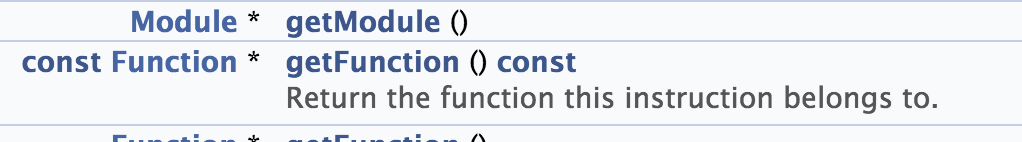
\includegraphics[scale=0.45]{pics/dox1.png} \newline
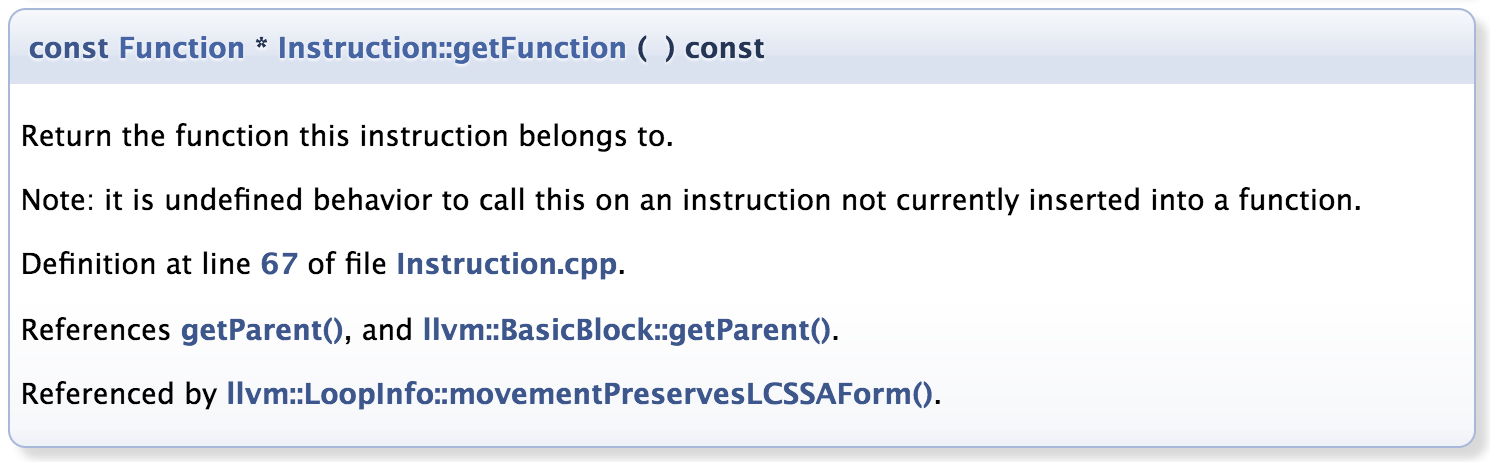
\includegraphics[scale=0.45]{pics/dox2.png} \newline

\end{itemize}


\subsubsection{Code Convention}
\begin{itemize}

\item Pointer and reference symbol is near to data type, not variable name.

\item Use \texttt{static\_assert} to test some compile-time boolean conditions. It support a message parameter. It doesn't need to build execution application. It will stop when you are compiling your code. 
\begin{lstlisting}[frame=single, language=c++]
static_assert(sizeof(int) > 4, "int is too small");
\end{lstlisting}

\item For forward function, 1) prefer to use reference 2) don't inline f function. Detail can be found in GotW27.

\begin{lstlisting}[frame=single, language=c++]
bool f( X& x ){
return g( x );
}
\end{lstlisting}

\item Use \texttt{const} as many as possible. Detail can be found in const section below. 

\item Declare variables as locally as possible and minimize usage of global data.

\item Avoid macro, use inline function;  Avoid magic numbers, instead of using \texttt{const} and \texttt{enum}

\item Format lambdas like blocks of code.
\begin{lstlisting}[frame=single, language=c++]
int cutoff = 7;
std::find(foo.begin(),foo.end(),[&](const Foo &a ) ->bool{
    return a.blah<cutoff  //use reference to get local var
});
\end{lstlisting}

\item \textbf{Always initialize variables.}  Some suggestions about initialization are below:
\begin{enumerate}
\item Manually initialize non-member objects of built-in types. including a pointer.
\item Use \textbf{member initialization list} to initialize all members inside an object.
\item The initialization order uncertainty that afflicts non-local static objects defined in separate translation units. The questions is below:

\begin{lstlisting}[frame=single, language=c++]
#include "x.h" // File x.cpp
X x;
//x maybe initialize before y or after y

#include "y.h" // File y.cpp
extern X x;
Y y;
Y::Y(){ //here x maybe not be constructed
  x.goBowling();
}
\end{lstlisting}

\item  How to resolve: build a singleton class
\begin{lstlisting}[frame=single, language=c++, mathescape=true]
#include "x.h"  // File x.cpp
X& getX(){
  static X x;
  return x;
  $\Hilight{30}$//another implementation.
  //static X* px = new X();
  //return *px;
}

#include "y.h" // File y.cpp
Y y;
Y::Y(){ //here x maybe not construct
  $\Hilight{4}$getX().goBowling();
}
\end{lstlisting}

\item Pay attention to the global object which are initialized in right order. Because the order can be arranged in the same translation unit, but not \textbf{between translation units}, see effective c++ Item 47. So we don't encourage you to use global object unless it's very necessary.

\item Even in the same translation unit, formally, C++ initializes static and global variables in three phases: 1. Zero initialization 2. Static initialization 3. Dynamic initialization

\begin{lstlisting}[frame=single, language=c++, mathescape=true]
int g0;  //zero initialization
int g1 = 42;    //  static initialization
extern int f();
int g2 = f();   //  dynamic initialization
\end{lstlisting}

\begin{lstlisting}[frame=single, language=c++, mathescape=true]
int a = f(); // a exists just to call f
int x = 22;
int f() {
    ++x;
    return 123; // unimportant arbitrary number
}
// x equals to 23, not 22
// bcause static initialization
is earlier than dynamic initialization
\end{lstlisting}

\end{enumerate}

\item Use \_FILE\_ and \_LINE\_ to capture the current file name and line number.  \texttt{assert} just uses this kind of macro inside.

\item Use \texttt{const} replace \texttt{\#define} to define global constants. \texttt{static const} can be used to define constant class member. (\texttt{const} means that it will not change, so I don't need keep multi copy in multi objs, so I use static.)

\item Use more typedef or alias to simplify Complicated Type Expressions, It's helpful especially in STL. 
 \begin{lstlisting}[frame=single, language=c++]
typedef std::map< int, int > IntMap;
typedef IntMap::const_iterator IntMapConstIter;
for( IntMapConstIter it = layout.begin();
                            it != layout.end(); ++it ) {

typedef int(*CB)(int, const char*); //C++11 use function<>
CB callBack;  //decare a functions pointer.

int sort(int, const char*){..}
callBack = sort; // & operator is optional here!
\end{lstlisting}

\item Using alias(C++11) is better than typedef. 
\begin{enumerate}
\item First word is \texttt{using}, \textbf{There are no sharp symbol before \texttt{using} .} 
\item Second is TypeName. 
\item Third is assignment \texttt{=}.  
\end{enumerate}

\begin{lstlisting}[frame=single, language=c++]
using UPtrMapSS =
std::unique_ptr<std::unordered_map<std::string, int>>;

using CB = int(*)(int, const char*);
\end{lstlisting}

\item Create a zero-valued enumerator to indicate an invalid or default state and make it the first item.

\item \textbf{Declare all member variables private, then use getter and setter functions to access them.}

\item Don't use multi-thread unless you really need it. Simultaneously respond to many events. Just remember, synchronization has some overhead. Below are some typical scenarios.
\begin{enumerate}
\item A web server.
\item Interface and working thread.
\item Take advantage of with multiple processor.
\end{enumerate}

\item \textbf{Uses early exits to simplify code.}

\begin{lstlisting}[frame=single, language=c++]
if(IsValid){   //bad style
   do something;
} else{
  return;
}

if(!IsValid)  // A better style is
  return;
..do something here.
\end{lstlisting}

\item Turn Predicate Loop into Predicate Function. It makes you code clean and easy to understand.

\begin{lstlisting}[frame=single, language=c++]
for(v.begin....){   /bad style
  if(it->IsSth){
      flag = true; break;
  }
}
if(flag){...}

// A better style is define isHasSth() return bool.
if(isHasSth()){...}
\end{lstlisting}

\item Use assert more in your project. You don't need to include file name and line number in the string. assert will output these hint messages.
\begin{lstlisting}[frame=single, language=c++]
#include<cassert>
assert(index>=0 && " index is negative");
//Assertion failed: expression, file name, line num
\end{lstlisting}

\item \textbf{If you don't modify container inside loop}, don't need to evaluate end() every time through for loop. Please remember below code block. \textbf{Just remember auto i,e ++i}
\begin{lstlisting}[frame=single, language=c++]
//g++ -std=c++11
vector<int> con={1,2,3}; //list initializer
for(auto i = con.begin, e = con.end();i!=e; ++i){
              ...........
}
\end{lstlisting}

\item The C++11 standard (§ 23.2.1) mandates that end has O(1) complexity, so previous item has no efficiency meaning in C++11.

\item A range-based for loop is introduced in C++11. Use auto\& to aoid copying each element. Below are highly recommended when yo use STL container.

\begin{enumerate}
		\item For observing the elements, use the following syntax:

\begin{lstlisting}[frame=single, language=c++]
for (const auto& elem : container)    
// capture by const reference
\end{lstlisting}
	\item If the objects are cheap to copy (like ints, doubles, etc.), it's possible to use a slightly simplified form:

\begin{lstlisting}[frame=single, language=c++]
for (const auto elem : container)   
// capture by value
\end{lstlisting}            

\item For observing the elements in generic code. since we can't make assumptions about generic type T being cheap to copy, it's safe to always use for (const auto\& elem : container).
(This won't trigger potentially expensive useless copies, will work just fine also for cheap-to-copy types like int, and also for containers using proxy-iterators, like std::vector<bool>.)

\item Of course, if there is a need to make a local copy of the element inside the loop body, capturing by value (for (auto elem : container)) is a good choice.

\begin{lstlisting}[frame=single, language=c++]
for (const auto& elem : container)
\end{lstlisting}

\item For modifying the elements in place, use:
\begin{lstlisting}[frame=single, language=c++]
for (auto& elem : container)    
// capture by (non-const) reference
\end{lstlisting}


\item Below code doesn't work, because std::vector template is specialized for bool, with an implementation that packs the bools to optimize space (each boolean value is stored in one bit, eight "boolean" bits in a byte). Because of that (since it's not possible to return a reference to a single bit), vector<bool> uses a so called "proxy iterator" pattern. A "proxy iterator" is an iterator that, when dereferenced, does not yield an ordinary bool \&, but instead returns (by value) a temporary object, which is a proxy class convertible to bool.
\begin{lstlisting}[frame=single, language=c++]
vector<bool> v = {true, false, false, true};
for (auto& x : v)
    x = !x;
\end{lstlisting}

\item If we want generic code to work also in case of proxy-iterators, the best option is for (auto\&\& elem : container).
(This will work just fine also for containers using ordinary non-proxy-iterators, like std::vector<int> or std::vector<string>.)
\begin{lstlisting}[frame=single, language=c++]
for (auto&& elem : container)
\end{lstlisting}

\item If there are pointer inside the container. You don't need star symbol explicitly, but it give more information to the variable, so I reccommend using it.
\begin{lstlisting}[frame=single, language=c++]
//make sure Container contain pointer
for(auto *ptr: Container){ ptr->change();}
for(const auto *ptr: Container){ ptr->read();}
\end{lstlisting}

\end{enumerate}

\item The range-based version is for: You want to do something with every element in the container, without mutating the container(insert or erase). If you want to mutate the container, Follow idea introduced in Container--Erasure section below.

\begin{enumerate}
\item For any container, you can \textbf{NOT} mutating container by calling insert or erase inside loop.
\item If you really want to change a container, for a sequential container, you can use range-based version change element. 
\item For any associate container, only visit each element.
\end{enumerate}


\item Common function interface: \textbf{you can see \texttt{const} only used in pointer or reference type. You should use more \texttt{const} in your projects. }

\begin{tabular}{|c|c|c|}
\hline
 \textbf{type} & \textbf{read} & \textbf{write} \\
\hline
primitive (char, int, float) & pass value & pointer or reference \\
\hline
class, array, structure  & const pointer or reference &  pointer or reference  \\
\hline
\end{tabular}

\item \textbf{Prefer Preincrement (++i), especially in a for loop.}  When you use ++i or i++ inside expression, there are differences. Otherwise, there is no differences.
\begin{lstlisting}[frame=single, language=c++]
for(int i = 0;i<10; ++i)
j=++i; // j = i+1;
j=i++; //j = i;  i=i+1;
++*p;  //++(*p) ;
*++p; //*(++p);
\end{lstlisting}

\item How to understand \texttt{*p++} ?

\begin{enumerate}
\item Precedence of prefix ++ and * is same. Associativity of both is right to left.
\item Precedence of postfix ++ is higher than both * and prefix ++. Associativity of postfix ++ is left to right.
\item Prefix and postfix are both syntax sugar, in order to reduce typing.   But prefix represents \textbf{one statement}, postfix means \textbf{two statements};
\end{enumerate}

\begin{lstlisting}[frame=single, language=c++]
++i;  //just like i = i+1 or  i+=1;
//when i++ used in expression, treated as two statements;
*p++; // *(p++);  *p ; p=p+1;

while(*p != '\0'){
p= p+1;
}
//can be written to
while(*p++ != '\0')
\end{lstlisting}

\item Always turn on all warning options in your compiler with -Wall. Once you get warning, Eliminate warning before you go further.

\item Sometimes, this warning is what you have to, or if warning comes from a header file you can't change. You can use \#pragma warning compile directive to temporary disable it, then restore it later.
\begin{lstlisting}[frame=single, language=c++]
#pragma warning(push)
#pragma warning(disable:4512);
#include<not_change.h>
#pragma warning(pop) //restore original warning level
\end{lstlisting}

\end{itemize}

\subsection{Basic of C and C++}
\subsubsection{Basic concepttion}
\begin{itemize}
\item C++ inherits basic data type, variable name, statement, expression, and operator, control flow, function, file, head file and library, array, pointer and structure from C language. C++ is subset of C, so any C programs can be compiled by C++. Compared with C language,  C++ include two extensions, one is \textbf{Template(Generic coding)} and the other is \textbf{OOP}.

\item Duration and scope are two different conceptions. there are three kinds of duration:
\begin{enumerate}
\item automatic 
\item static 
\item dynamic. 
\end{enumerate}
there are three kinds of scopes:
\begin{enumerate}
\item global
\item In C++, we can use namespace to add more scopes to divide global scope.
\item file(translation unit)
\item local
\item 
\end{enumerate}

\end{itemize}



\subsubsection{Combine C and C++}
\begin{itemize}

\item When you use g++,  \_\_cplusplus will be defined automatically. (you can't undef it in fact.) When you use gcc, \_\_cplusplus is not defined. At the same time, When you use g++ to compile a C file, although file extension is .c, but g++ still use name mangling to change function name.  (The conclusion is based on g++ and gcc on Linux system)

\item If you have c and cpp source files together, you can just use g++ compile them all. You don't need any \_\_cplusplus syntax.  g++ compile all files using name mangling. (look them as c++ files). At this time file extension doesn't play a role at all.

\item If you c++ file want to use a c function. You don't have c function source code(It is in a lib or obj file) or you don't want to recompile it( it's a very big C library). At this time, you should use " extern "C" " in head file or function declaration.
\begin{lstlisting}[frame=single, language=c++]
#ifdef __cplusplus
extern "C" {
#endif

Foo (int a, int b);

#ifdef __cplusplus
}
#endif
\end{lstlisting}

\item If you define a function in a.cpp file(You have to use g++ to compile it), and this function will be used in legacy C system, you need the previous trick again.  You can give lib and head file to C system,  and then the C system can include head file and linked to lib.

\item \textbf{In one word, if you have obj code produced by C or C++, When you want to linked it to current different language, you should consider using "\_\_cplusplus" }
\item There are three occasions which you need to use extern C
		\begin{enumerate}
				\item When you want to produce a DLL or SO. Why, because maybe your DLL or SO will be used in C language or different compiler which use different name mangling rule.
				\item When the code will be used by java or python.
				\item When used with legacy C code.
		\end{enumerate}

\end{itemize}

\subsubsection{Translation unit}

\begin{itemize}

\item When you write an implementation file (.cpp, .cxx, etc),  your compiler generates a translation unit. This is the object file from your implementation file plus all the headers you \#include in it.

\item Each .cpp is a translation unit. Basically, you should put each class into a single .cpp file, and make sure each .cpp file has a corresponding .h file.  If two classes are highly correlated, they maybe be put in the same .cpp file.

\item A translation unit roughly consists of a source file after it has been processed by the C preprocessor, meaning that header files listed in \#include directives are literally included, sections of code within \#ifdef may be included, and macros have been expanded.

\item If you just want a function or variable visible to only current translation unit. You can declare it as static. Or you can use unnamed namespace.  You don't need to put it into a header file.  But in C++, you have to declare function and variable before you use them. Different with C language, In C language, compiler will guess a function prototype from it's usage, It's not good most of time.

\item C/C++ use separate compilation. If you need to use a function or variable in two different files, you should put them in the  global.h file and include them when necessary. (add extern keyword before variable name).  It will keep declaration just once, \textbf{DO NOT copy declaration to the other positions in the other .cpp file. It will lead to many duplication, it's bad smell of code.}

\item In your project, you can global search function or varaible declaration, if you find more than two, It's strong indication to make a global head file and put it into it. A better suggestion is to have a single global.h file for a complex system. Then put some common type, defined type, constant and global function in this single global.h file. So it will help to reduce duplication, just keep once appearance.

\item Three rules about header file:

\begin{enumerate}
\item Use \textbf{\#pragma once} to add include guard, It's not standard, but It has been supported by many compiler. Including g++, clang and MSVC.

\item \textbf{Put your local/private header file in front of system header file. }  Why? There are two advantages, 1) You can know what header file should be included, It's helpful to achieve the goal of demand 2.  2) Sometimes, if you have you own function with same name as system or library, It can give you a compile error; Below example will give you a compile error. But if you put <cmath> before myHead.h. Then, main will use acos in cmath, and your acos will be override.

\begin{lstlisting}[frame=single, language=c++]
#include "myHead.h"  //double acos(double)
#include <cmath>
main{
acos(0.5);
}
\end{lstlisting}

\item You will need to put the minimal set of \#include statements that are needed to make the header compilable when your local/private header is included on the first place.  It will make your header file self-sufficient.
\end{enumerate}

\item In .h file, you can include template and inline function.  In fact, you have to put template into .h file. 

\item \textbf{Putting a semicolon in the end of head file is good suggestion.} You also need semicolon after declare class. In .cpp file, no semicolon after each function definition.

\end{itemize}

\subsubsection{Declaring and definition}
\begin{itemize}

\item A declaration introduces an identifier and describes its type, be it a type, object, or function. \textbf{A declaration is what the compiler needs to accept references to that identifier.} 

\begin{lstlisting}[frame=single, language=c++]
extern int bar;
extern int g(int, int);
double f(int, double); 
// extern can be omitted for function declarations
class Foo; 
// no extern allowed for type declarations
\end{lstlisting}

\item A definition actually instantiates/implements this identifier. It's what the linker needs in order to link references to those entities. These are definitions corresponding to the above declarations:
\begin{lstlisting}[frame=single, language=c++]
int bar;
int g(int lhs, int rhs) {return lhs*rhs;}
double f(int i, double d) {return i+d;}
class foo {}; //put ; after calss definition.
\end{lstlisting}

\item The difference between declaring a symbol and defining a symbol: A declaration tells the compiler about the existence of a certain symbol and makes it possible to \textbf{refer to that symbol everywhere where the explicit memory address or required storage of that symbol is not required.}  A definition tells the compiler what the body of a function contains or how much memory it must allocate for a variable.

\item One very important difference between declarations and definitions is that a symbol may be declared many times, but defined only once. For example, you can forward declare a function or class however often you want, but you may only ever have one definition for it. This is called the \textbf{One Definition Rule}.

\item Even you can declare variable, function and class many times, it's not good smell to do that.  If you modify it's name, you need to trace back all the declaration. \textbf{If a function or class is used by many units, You'd better build a global header file "global.h". and put all the declaration there.} 

\item In C++, there exists the concept of forward declaring a symbol. We declare the type and name of a symbol so that we can use it where its definition is not required. A direct usage is PIMPL. 
\begin{enumerate}
\item It will reduce compile-time dependencies.
\item Hide all the detail. 
\item Break cyclic references
\end{enumerate}

\begin{lstlisting}[frame=single, language=c++]
// file.hpp
class C1; // that is forward declaring.

class C2{
...
C1* pc1;
}
\end{lstlisting}

\item About pimpl, you need to know below:

\begin{enumerate}

\item In you .h file, when you use Foo* p or Foo\& rp; You don't need include Foo.h file. you can use forward declaration.
\begin{lstlisting}[frame=single, language=c++]
class Foo;
Foo* p;
\end{lstlisting}

\item Base on previous forward declaration, you can use "Pimpl" idiom.
\begin{lstlisting}[frame=single, language=c++]
// widget.h file
class Widget { // still in header "widget.h"
private:
struct Impl; // declare implementation struct
std::unique_ptr<Impl> pImpl;
};

//widget.cpp file
#include "Foo.h"  // just include Foo.h in .cpp file.
struct Widget::Impl {
Foo f1;
Gadget g1;
};
\end{lstlisting}


\item Pimpl Idiom is one of std::unique\_ptrs most common use cases. But different with raw pointer,  you need to declare or implement some special member functions, such as dtor ctor and move ctor. Explanation can be seen in "effective modern C++ item 22". 
\begin{lstlisting}[frame=single, language=c++, mathescape=true]
// widget.h file
class Widget { // still in header "widget.h"

Widget(Widget&& rhs); // declarations
Widget& operator=(Widget&& rhs); // only
$\Hilight{12}$Widget::~Widget()
Widget(const Widget& rhs); // declarations
Widget& operator=(const Widget& rhs); // only

private:
struct Impl; // declare implementation struct
std::unique_ptr<Impl> pImpl;
};

//widget.cpp file
#include "Foo.h"  // just include Foo.h in .cpp file.

Widget::~Widget() = default; // as before
Widget::Widget(Widget&& rhs) = default; // definitions
Widget& Widget::operator=(Widget&& rhs) = default;
Widget::Widget(const Widget& rhs) // copy ctor
: pImpl(std::make_unique<Impl>(*rhs.pImpl))
{}

Widget& Widget::operator=(const Widget& rhs) {
*pImpl = *rhs.pImpl;
return *this;
}
\end{lstlisting}

\end{enumerate}

\item Forward declartion doesn't work if you need to build or access its member. It's only work when you refer it by pointer or reference.

\begin{lstlisting}[frame=single, language=c++]
class Foo;
Foo* f1 = new Foo //error, you need #include Foo.h
// so compile can know all detail.

fun(Foo* f1){
f1->a; 
//error, compiler need to know if there is a 
}
fun(Foo f1) //error, compiler need to know the size.
\end{lstlisting}
\end{itemize}

\subsubsection{ODR}
\begin{itemize}

\item For C langauge, there is tenttive defintion rule. You can define the same varaible in two different .c file. The result will be undefined. But in the C++, this is not allowed any more. 

\begin{lstlisting}[frame=single, language=c++]
a.c
int g_i = 100;
////////////////////////////////
b.c
int g_i;
fun(){
printf("%d",g_i) //will print 100
//gcc a.c b.c report no error.
//g++ report error
//in b.c, if you g_i= 2; gcc report error.
\end{lstlisting}

\item For C++ langauge ,tentative defintion of varialbe is not allowed. At the same time, multi-definition of function is not allowed either. but there are another implicit risk as below. 

\item In the same unit, you can't define class C1 again, but if you put two class C1 in two different .cpp file. compiler will not complain at all. When you run you application probably crash, it's dangerous. It's a little different with function and global variable. Because function and global varaible all need allocation memory.

\item \textbf{Either a name is for everyone (and declared in a header file) or is translation-unit-local in an anonymous namespace.} Detail can be found in "The One-Definition Rule  Andrzej's C++ blog".

\item  If an inline function appears in foo.cpp (either because it was written in it, or because it \#includes a header in which it was written, in which case the preprocessor basically makes it so). Now you compile foo.cpp, and possibly also some other bar.cpp which also contains an inline function with the same signature (possibly the exact same one; probably due to both \#includeing the same header). When the linker links the two object files, it will not be considered a violation of the ODR, as the inline directive made each copy of the file local to its translation unit (the object file created by compiling it, effectively). This is not a suggestion, it is binding.

It is not coincidental that these two things go together. The most common case is for an inline function to appear in a header \#included by several source files, probably because the programmer wanted to request fast inline expansion. This requires the translation-unit locality rule, though, so that linker errors shouldn't arise.

\item \textbf{Put inline function into the header file.}
\end{itemize}

\subsubsection{Linkage}
\begin{itemize}
\item scope is a property handled by compiler, whereas linkage is a property handled by linker.

\item Another property of internal linkage is that it is only implemented when the variable has global scope. static has internal linkage. non-const global variable has external linkage. All constants are by default internally linked. So you can put \texttt{const int g\_num = 10;} into a global header file, but you can't put a static variable into the global header file.

\item const variables internally link by default unless otherwise declared as \texttt{extern}. It means that:

\begin{enumerate}
\item You can put \texttt{const int g\_num = 10;} into a header file or global.h file. Then when you need g\_num, just include this header file into you .cpp and it will not cause redefine linkage error.

\item You can put \texttt{const int g\_num = 10;} in one .cpp file. then declare \texttt{extern const int g\_num ;} in global.h file.

\item \textbf{For const used just in one .cpp, use static and put it in the .cpp file.}
\end{enumerate}

\item Internal linkage refers to everything only in scope of a translation unit.

\item External linkage refers to things that exist beyond a particular translation unit. In other words, accessible through the whole program, which is the combination of all translation units (or object files).

\item When internal linkage, it means that 1) you can put two same static varaible name in two different .cpp file, no linkage error. 2) you can't put extern before static, in another word, you can't access static variable in another .cpp file. 
\end{itemize}

\subsubsection{vexing parsing}
\begin{enumerate}
\item Use parentheses to group when you declare a variable. \textbf{When you declare something, It's legal to use parentheses to group varaible name.} Sometimes, you have to use parentheses, such as declare a function pointer. 
\begin{lstlisting}[frame=single, language=c++, mathescape=true]
int f(int);   //a function return a int
int *f(int);  //a function.return pointer
int (*f)(int); // function pointer;  
\end{lstlisting}

\item It means that you can have below C++ statements. 
\begin{lstlisting}[frame=single, language=c++, mathescape=true]
int x;
int (x); //same as above
int f(int x);
int f(int (x)); //same as above
\end{lstlisting}

\item For function declaration, you can omit the parameter name.  
\begin{lstlisting}[frame=single, language=c++, mathescape=true]
int f(int x);
int f(int (x));
int f(int); //three statements are same. 
\end{lstlisting}

\item For object, thing becomes interesting.
\begin{lstlisting}[frame=single, language=c++, mathescape=true]
int (x); // just like int x;

class A{
A(int a);
...}

A(a);  // You want to create a temporary obj
//but compile think it as A a;

(A(a)); 
//If you really want a temporary A object,
//use another parentheses. 
\end{lstlisting}

\item For function, vexing problem happen below.
\begin{lstlisting}[frame=single, language=c++, mathescape=true]
int f(double (*pf)()); //standard way
int f(double pf()); //You can omit parentheses
                    // just like int x and int (x);
int f(double ()); for function f, you can omit variable name.                 
 \end{lstlisting}

\item Based on all above all the knowledges. We have a complex problem.
\begin{lstlisting}[frame=single, language=c++, mathescape=true]
struct A{
    A (B const& b){};
    void doSomething(){};
};
 
int main(){    
    A a(); // declare a function "a", return A
    
    A a(B(x)); //declare a function "a",   
               //type of parameter x is B
               
    A a(B()); //declare a function "a",
//receive function pointer, return B, void input
and parameter name for "a" is omitted.   
\end{lstlisting}

\item In previous example, Why B(x) equal B x; but B() equal a function pointer? If B(int), then it will be a function pointer.  function declaration need type name, not a variable name, such as x.

\item The most complex problem. A range container constructor. 
\begin{lstlisting}[frame=single, language=c++, mathescape=true]
list<int> data(istream_iterator<int>(dataFile), 
                istream_iterator<int>()); 
// data is function. first parameter is dataFile, type istream_iterator<int>
// second parameter is function pointer. 
\end{lstlisting}

\item Before C++11, you need add another pair parentheses to change it from declaration to expression. After C++11, you can use braces.
\begin{lstlisting}[frame=single, language=c++, mathescape=true]
A a{B{x}}; 
A a{B{}};
\end{lstlisting} 

\item A non-static data member initializer (NSDMI) must use a brace-or-equal-initializer.
\begin{lstlisting}[frame=single, language=c++, mathescape=true]
class A{
  int equals = 42;                      // OK
  std::unique_ptr<Foo> braces{new Foo}; // Also OK
  std::vector<int> bad(6);  // not allow
  std::vector<int> good{6}; // OK  
}  
\end{lstlisting}

\end{enumerate}

\subsection{malloc and remalloc}
\subsubsection{malloc}
\begin{itemize}
\item That is a long story. In C language, if you forget a header file, what will happen? (I have add answer to my evernote). In one word, It will(c99) or will not produce(c89) warning, and compiler will assume a "implicit int" rule. That is to say, It presumes that the function without prototype (declaring in the header file) just return int type.

\item continue: if you have code below: you comment stdlib.h. Then compiler will assume that malloc return a int.  This code will run on 32 bit computer, because int and int* have same length. but on some 64 bit computer, int* is 64 bit and int is 32 bit.  so half data will be lost, and you code will crash.
And if you add (int*) cast, it will suppress the warning message.(You kill the only clue, it's bad).
 \begin{lstlisting}[frame=single, language=c++]
 // include "stdlib.h"
// with cast, it will NOT produce a (missing protype)warning.
int *sieve = (int *)malloc(sizeof(int)*length);

// without cast, will produce a warning.
int *sieve = malloc(sizeof(int)*length);
\end{lstlisting}

\item continue: So don't recommend to use (int*) cast at all. Next question is that malloc actually return void*. Can void* automatically implicit be cast to int* or other pointer type in assignment? the answer is \textbf{YES}.

\item  continue: In C language:
 \begin{lstlisting}[frame=single, language=c++]
#define NULL ( (void*) 0)
int *p = NULL;  //legal
FILE * f = NULL;  //legal
\end{lstlisting}

\item continue: In C++, int *p = (void *) 0 is not legal any more.(C++ is type safe language).  So in C++ NULL is literal 0. But It produce another ambiguity problem.  So In C++11, we define nullptr to resolve this problem.
 \begin{lstlisting}[frame=single, language=c++]
#define NULL 0
int *p = NULL //legal
--------------------------------------
f(int i)
f(int * p);

f(NULL);  //which one will be called. Answer is f(int i).
f(nullptr) //will call f(int *p)
\end{lstlisting}

\item calloc() zero-initializes the buffer, while malloc() leaves the memory uninitialized. Zeroing out the memory may take a little time, so you probably want to use malloc() if that performance is an issue. If initializing the memory is more important, use calloc(). For example, calloc() might save you a call to memset().
\end{itemize}

\subsubsection{realloc}
\begin{itemize}
\item Don't return value assign to input ptr, use another local pointer, such as new\_ptr;
 \begin{lstlisting}[frame=single, language=c++]
void *new_ptr = realloc(ptr, new_size);
if (!new_ptr) {
    // deal with error;
}
ptr = new_ptr
\end{lstlisting}
\end{itemize}


\subsection{new operator}
\subsubsection{basic}
\begin{itemize}

\item There are four parts of knowledge about new operator:
\begin{enumerate}
\item new\_handler
\item no throw, but return nullptr(since c++11)
\item placement new (not allocate, just ctor)
\item operator new (just allocate, no ctor)
\end{enumerate}

\begin{lstlisting}[frame=single, language=c++]
std::set_new_handler(noMem);
MyClass * p1 = new MyClass;  //1: if fail, call noMem

MyClass * p2 = new (std::nothrow) MyClass; //2: no throw

new (p2) MyClass;  //3: placement new

//4: operator new
MyClass * p3 = (MyClass*) ::operator new (sizeof(MyClass));
      // allocates memory by calling: operator new
      // but does not call MyClass's ctor
\end{lstlisting}

\item \texttt{new} will call constructor function of a class, but \texttt{malloc} will not call constructor function.  \textbf{So in C++, you should use new instead of \texttt{malloc}.}

\item If you use new int[100], use delete [];  \textbf{Any time you want to use new to allocate an array, ask yourself if you can replace it with vector or string.}
\end{itemize}

\subsubsection{Inside of new}
\begin{itemize}
\item Source code of new operator and delete operator.
\begin{enumerate}
\item call operator new to allocate space in memory.
\item call ctor of a class.
\item If you want to allocate memory, call operator new, not new opeator, in this way, ctor will not be called.

\begin{lstlisting}[frame=single, language=c++]
Foo* p;
 // don't catch exceptions thrown by the allocator itself
 // Return a void type pointer
 void* raw = operator new(sizeof(Foo)*100);

p = new (std::no_throw) Foo(); 

 // catch any exceptions thrown by the ctor
 try {
   p = new(raw) Foo();  // call the ctor with raw as this
 }
 catch (...) {
   // oops, ctor throw an exception
   operator delete(raw);
   throw;  // rethrow the ctor's exception
 }
\end{lstlisting}

\item Source code of delete operator. So for a class, if you declare its dtor private or protected, You can't use "delete p".
\begin{lstlisting}[frame=single, language=c++]
/* delete operator */
if (p != NULL) {
  p->~Foo();
  operator delete(p);
}
\end{lstlisting}
\end{enumerate}

\item You can't change "new operator" behavior, but you can override global "operator new" and overload class its own "operator new". Pay attention its argument and return void*. 

\begin{lstlisting}[frame=single, language=c++, mathescape=true]
//global operator new
$\Hilight{4}$ void* operator new($\Hilight{7}$size_t size){
   cout<<"Yan's own operator new" ;
   void* mem = malloc(size);
   if(mem)
      return mem;
   else
     throw bad_alloc();
}

class Foo{ //class operator new
public:
static void* operator new(size_t size);
// use $\Hilight{4}$ static
}

void* Foo::operator new(size_t size){
   cout<<"Foo's own operator new";
   ....
}

int *p = new int[100]; //output Yan's own operator new
Foo* fp = new Foo();  //output Foo's own operator new
\end{lstlisting}

\item Above code is just a simple demo, In the new\_handler section, you can see a better operator new demo with support of call your own new\_handler. You need to combine above code and code in new\_handler section together. 

\item operator new usually call \texttt{malloc} function. \texttt{malloc} usually call \texttt{brk} for small chunk and \texttt{mmap} for big chunk. So in the end, C langauge is basic langauge.

\item Why do I need my own operator new?
\begin{enumerate}
\item Performance: the default memory allocator is designed to be general purpose. Sometimes you have very specific objects you want to allocate, chapter 4 in "Modern C++ Design" presents a very well designed and implemented custom allocator for small objects.

\item Debugging \& statistics: having full control of the way memory is allocated and released provides great flexibility for debugging, statistics and performance analysis.

\item Customization to cluster related object together, and reduce size. put guard block to avoid overrun and underrun. More detail can be seen in effective c++( third edition) Item 50
\end{enumerate}

\item \textbf{Don't rewrite operator new unless you have to.} There are not as easy as you think. such as alignment. First consider some library, such as \textbf{Boost Pool library} for large number small object allocations. 

\item If you have to rewrite operator new, You need to read  effective c++( third edition) Item 51 in detail. For example, All operator new should contain a loop calling a new-handling function.  should deal with request of zero size. you can see the pseudocode in Item 51.

\item In C++, after you define a name in a scope (e.g., in a class scope), it will hide the same name in all enclosing scopes (e.g., in base classes or enclosing namespaces), and overloading never happens across scopes. And when said name is operator new, If you provide any class-specific new, provide all of the standard forms(plain, in-place, and nothrow)
\begin{lstlisting}[frame=single, language=c++, mathescape=true]
class C {
static void* operator new(size_t, MemoryPool&);
// hides three normal forms
};
$\Hilight{12}$//1) plain new
void* operator new(std::size_t);
$\Hilight{12}$//2) nothrow new
void* operator new(std::size_t, std::nothrow_t) throw();
$\Hilight{12}$//3) inplace new
void* operator new(std::size_t, void*);
\end{lstlisting}

\item Always provide new and delete together, see "C++ coding standards" item 45 and 46.
\end{itemize}

\subsubsection{new\_handler}
\begin{itemize}
\item  The new-handler function is the function called by allocation functions whenever a memory allocation attempt fails. Its intended purpose is one of three things:

\begin{enumerate}
\item make more memory available. \textbf{resolve the problem by myself.}

\item throw exception of type std::bad\_alloc or derived from std::bad\_alloc. \textbf{resolve the problem by a user.}

\item terminate the program. e.g. by calling std::terminate. \textbf{(No resolve)}
\end{enumerate}

\item At program startup, new-handler is a null pointer. allocation function finds that std::get\_new\_handler returns a null pointer value, it will throw \texttt{std::bad\_alloc}.

\item The default implementation throws \texttt{std::bad\_alloc}. The user can install his own new-handler, which may offer behavior different than the default one.

\item If new-handler returns, the allocation function repeats the previously-failed allocation attempt and calls the new-handler again if the allocation fails again. To end the loop, new-handler may call std::set\_new\_handler(nullptr).

\item Use set\_new\_handler function. When memory allocate failed, it will call this "callback" function.
\begin{lstlisting}[frame=single, language=c++]
void noMemory(){
closeIE; // method 1 release mem
set_new_handler(nullptr); //mehtod 2 throw bad_alloc exception.
abort();  //method 3, end application.
}
//in the beginning of main() function.
set_new_handler(noMemory)
\end{lstlisting}

\item What can we do in side new handler function? Below choices give you considerable flexibility in implementing new-handler functions.
\begin{enumerate}

\item Make more memory available. This may allow the next memory allocation attempt inside operator new
to succeed. One way to implement this strategy is to allocate a large block of memory at program start-up, then release it for use in the program the first time the new-handler is invoked.

\item Install a different new-handler. If the current new-handler can't make any more memory available, perhaps it knows of a different new-handler that can. If so, the current new-handler can install the other new-handler in its place (by calling \texttt{set\_new\_handler}). The next time operator new calls the new-handler function, it will get the one most recently installed. (A variation on this theme is for a new-handler to modify its own behavior, so the next time it's invoked, it does something different. One way to achieve this is to have the new-handler modify static, namespace-specific, or global data that affects the new-handler's behavior.)

\item Deinstall the new-handler, i.e., pass the null pointer to \texttt{set\_new\_handler}. With no new-handler installed, operator new will throw an exception when memory allocation is unsuccessful.

\item Throw an exception of type \texttt{bad\_alloc} or some type derived from \texttt{bad\_alloc}. Such exceptions will not be caught by operator new, so they will propagate to the site originating the request for memory.

\item Not return, typically by calling abort or exit.
\end{enumerate}

\item For a class, If you overload its own operator new, you also can overload its own new handler function. Detail can be found itme 49 in "Effective C++ third edition". 

\item An example code of operator new.

\begin{lstlisting}[frame=single, language=c++]
void * operator new(std::size_t size) throw(std::bad_alloc){                      
                    // your operator new might
using namespace std; // take additional params

  if (size == 0) {   // handle 0-byte requests
    size = 1;              // by treating them as
  }                 // 1-byte requests
  while (true) {
      attempt to allocate size bytes;
      if (the allocation was successful)
           return (a pointer to the memory);

      // allocation was unsuccessful; find out what the
      // current new-handling function is (see below)
     $\Hilight{35}$new_handler globalHandler = set_new_handler(0);
     $\Hilight{30}$set_new_handler(globalHandler);

     if (globalHandler) (*globalHandler)();
     else throw std::bad_alloc();
   }
}
\end{lstlisting}

\begin{enumerate}
\item set\_new\_handler are called twice, just for getting current new handler function pointer.

\item current new handler can't accessed directly, just like private member inside a class. So we need to use set/get idiom. Detail can be found "C++ gotchas" Item 80.
 
\item In C++11, introduce get\_new\_handler() function. We don't need to call set\_new\_handler twice.

\item This set/get idiom is also used in set\_terminate and set\_unexpect. 

\item Calling this function does not introduce data races, and any such call is synchronized with subsequent calls to set\_new\_handler and get\_new\_handler. About data races, you can see concurrent chapter.
\end{enumerate}

\end{itemize}

\subsubsection{placement new}

\begin{itemize}
\item construct an object in memory you've already got a pointer to ,use placement new. If you use placement new to create an object in some memory, you should avoid using the delete operator on that memory.  Detail can be seen in C++ primer
\begin{lstlisting}[frame=single, language=c++]
p1 = new(buffer) FOO();
p2 = new(buffer+sizeof(FOO) ) FOO();

p1->~FOO(); // call dtor directly,
p2->~FOO(); //don't call delete p1.

delete[] buffer;
\end{lstlisting}

\item A good article is "The many faces of operator new in C++", It give  detail information about operator new and how to rewrite it. I have added it to my ref.
\end{itemize}


\subsection{Numerical Overflow}

\begin{itemize}
\item Integer type has \textbf{overflow} problem, and float has \textbf{precision} problem. So prefer to use \textbf{long long} and \textbf{double} as your numerical type.

\item In C and C++, you can use limits.h or <limit> to get the all the type limit information.
\begin{lstlisting}[frame=single, language=c++]
INT_MAX //use in C
INT_MIN
//use in C++
cout<< std::numeric_limits<int>::lowest() << '\t'
cout<< std::numeric_limits<int>::max() << '\n';
\end{lstlisting}

\item For integer addition or subtraction, It just a round-trip. When you reach a position in the circle, how to understanding depends on its context and type.

\begin{lstlisting}[frame=single, language=c++]
unsigned int ui = 1;
int i = -2;
// i+ui will stop in one position in the round clock.
//how to interpret it depends on the programe context;
int j = i+ui; // as int interpret this position CORRECT
(ui+i)<6 //  as unsigned interpret this position. ERROR!
\end{lstlisting}

\item Most unsigned implicit cast error happen when you compare with a constant number. 

\item  Judge it before calculation.
\begin{lstlisting}[frame=single, language=c++]
if ((x > 0) && (a > INT_MAX - x)) /* `a + x` would overflow */;
// a is point, x>0 clockwise turn, then it will overflow

if ((x < 0) && (a < INT_MIN - x)) /* `a + x` would underflow */;
// a is point, x<0 anti-clockwise turn,  so it will underflow
//It's easy to understand if you draw a clock figure.

if ((x < 0) && (a > INT_MAX + x)) /* `a - x` would overflow */;
if ((x > 0) && (a < INT_MIN + x)) /* `a - x` would underflow */;

if (a > INT_MAX / x) /* `a * x` would overflow */;
if ((a < INT_MIN / x)) /* `a * x` would underflow */;
// need to check for -1 for two's complement machines
if ((a == -1) && (x == INT_MIN)) /* `a * x` overflow */
if ((x == -1) && (a == INT_MIN)) /* `a * x` (or `a / x`) overflow */
\end{lstlisting}

\item Judge it after calculation
\begin{lstlisting}[frame=single, language=c++]
uint32 a,b;
//assign values
uint32 result = a + b;
if (result < a) {
    //Overflow
}
\end{lstlisting}

\item Build your own template function.
\begin{lstlisting}[frame=single, language=c++]
template <class T>
void increment_without_wraparound(T& value) {
   if (value < numeric_limits<T>::max())
     value++;
}
\end{lstlisting}

\item There's no simple, general, portable way to avoid integer overflow.
\item You cannot safely check whether a signed integer addition or subtraction overflowed after the fact. An overflow in signed arithmetic causes undefined behavior. Typically the result wraps around, but in principle your program could crash before you have a chance to examine the result.

\item Clang 3.4+ and GCC 5+ offer checked arithmetic builtins. They offer a very fast solution to this problem, especially when compared to bit-testing safety checks.
\begin{lstlisting}[frame=single, language=c++]
unsigned long b, c, c_test;
if (__builtin_umull_overflow(b, c, &c_test)){
    // returned non-zero: there has been an overflow
}
\end{lstlisting}

\item When you do some calculation, you can have some tricks to avoid overflow. n! the last three digit. You need use mod to keep last two digits in each calculation.
\begin{lstlisting}[frame=single, language=c++]
(a+b)/2  //a+b maybe overflow
a/2+b/2 +(a&b&1);
\end{lstlisting}

\end{itemize}


\subsection{Numerical conversions}

\begin{itemize}
\item Three kinds of type conversions:
\begin{enumerate}
\item Assign a value of one \textbf{arithmetic type} to a variable of another arithmetic type.
\item Combine mixed types in expressions
\item Pass arguments to function.
\end{enumerate}

\item For basic data type(numeric), There are two possibilities: promotion and conversion.

\item There are two kinds of conversion, one is \textbf{implicit}, and the other is \textbf{explicit}.
\end{itemize}

\subsubsection{Numerical Conversion}
\begin{itemize}
\item Assigning a value to a type with a greater range usually poses no problem. If shorter range or different type, maybe there are some problems.

\item Assigned to a bool, zero will convert to false, and nonzero will convert to true.

\item When conversion, maybe lost precision(double -> float, long long ->float) loss fragment(float -> i) or Undefine (int i = 666, then char c = i;). Detail example can be seen in my evernote bookmark.

\begin{lstlisting}[frame=single, language=c++]
int i, float f;
i=f;
//1) fragment will be lost,  f= 3.99, i will be 3 (not rounding)
//2) If f is too big.  undefined behave

f = i;
// 1) will lost precision if i is big.
\end{lstlisting}

\item A implicit conversion will happen when you call a function.(Just like you use assignment operator=). Below they all compile successfully. 
\begin{lstlisting}[frame=single, language=c++]
bool isLucky(int number);

isLucky('a') //i = 'a' , promotion
isLucky(false) //i = false, promotion
isLucky(1.2f) //i = f , standard conversion.
\end{lstlisting}

\item Compile with -Wconversion flag, it doesn't included in -Wall in g++; It just give warning when standard conversion happen. (no warning for promotion  conversion).

\begin{lstlisting}[frame=single, language=c++, mathescape=true]
isLucky('a') //promotion, $\Hilight{2}$NO warning
isLucky(false) //promotion, $\Hilight{2}$NO warning
isLucky(1.2f) //standard conversion, Warning
\end{lstlisting}

\item In C++, introduce braces initialization \{\}, It will not allow narrowing happen. But in g++, it just show a -Wnarrowing message, Anyway, I think that it's helpful.
\begin{lstlisting}[frame=single, language=c++]
int x = 66;
char c1 = {x}; //ok

int x = 666;
char c2 = {x};  // not allowed;
\end{lstlisting}

\item When an operation involves two types, the smaller is converted to the larger. Adding an int to a float, int is converted to float type. (You have to do it, because two types have the different inside binary representations.)

\item In an expression, C++ makes two kinds of automatic conversion. 1) Some type are automatically converted whenever they occur. 2) Some type are converted when they are combined with other types in an expression.

\item C++ converts bool, char, unsigned char, signed char and short to int. Because int type is generally chosen to be the computer's most natural type. \textbf{It does calculations faster for that type.} It's called \textbf{integer promotions.}

\item unsigned short convert to int if short is shorter than int, if they have the same size. unsigned short convert to unsigned int.  So no data loss in promoting.
\begin{lstlisting}[frame=single, language=c++, mathescape=true]
char c1, c2, c //c1 and c2 convert to int first.
c = c1+c2;  // then change int result back to char.
/*  LLVM IR code below
  store i8 97, i8* %c1, align 1
  store i8 2, i8* %c2, align 1
  %0 = load i8, i8* %c1, align 1
  %conv = $\Hilight{3}$sext i8 %0 to i32
  %1 = load i8, i8* %c2, align 1
  %conv1 = sext i8 %1 to i32
  %add = add nsw i32 %conv, %conv1
  %conv2 = $\Hilight{3}$trunc i32 %add to i8
*/

i+f // i will promoted to f and value keep the same.

float f1, f2, f
f = f1+f2 // whether f1 change to double debpends on compiler
//clang++ has fadd in LLVM IR, so it doesn't change f to double.
\end{lstlisting}
\end{itemize}

\subsubsection{Explicit numerical conversion}
\begin{itemize}
\item In order to depress conversion warning, you can use explicit numerical conversion to state your intention clearly and loudly.

\item In C language, there exist two main syntax for generic type-casting: functional and C-style cast.  \textbf{Prefer C-style cast}

\begin{lstlisting}[frame=single, language=c++, mathescape=true]
double x = 10.3;
int y;
unsigned int n1 = (unsigned int)f; $\Hilight{10}$// C-style cast
unsigned int n2 = unsigned(f);     // functional cast
//functional cast only be used in one word type.
//unsigned int (f)  is not right,
//int *(f) is not right either.
\end{lstlisting}

\end{itemize}

\subsection{Type cast in c++}

\subsubsection{Implicit conversion in C++}
\begin{itemize}
\item Compiler will first match function name and number of arguments, then look for template deducted function, then use implicit conversion to try match. So implicit conversion happens after template.

\item When will class implicit convert. 1) single ctor, 2) operator Type.
\begin{lstlisting}[frame=single, language=c++]
class A {
A(int i); // bad
operator const char*(); //bad
};

A a1, a2;
a2 = a1*2;  //implicit conversion 2 to temp A obj
a2 = 2  the same, then call operator =;
\end{lstlisting}

\item \textbf{You should always avoid implicit conversion}
\begin{enumerate}
\item use explicit before single parameter ctor.
\item use name convert function instead of  "operator Type".so string has function c\_str() instead operator char*() const. 
\end{enumerate}

\item In an example below, with explicit keyword before ctor,  you have to use A(2) or (A)2 to explicitly build a A temperory obj in a1*A(2) expression.
\begin{lstlisting}[frame=single, language=c++]
class A {
explicit A(int i); // good
const char* getInternalPoint() ;
//good, use a name function.
};
\end{lstlisting}

\item  convert class to basic type, you need operator basicTypeName, no argument, no return value and member function.

\item Implicit conversion can be called by compiler implicit, (means that you don't know at all). It sometimes will lead to potential ambiguity problem.
\begin{lstlisting}[frame=single, language=c++]
class A{
A(class B&);
};
class B{
operator A()
};

void g(const A&);
B b;
g(b)
// it can call A's ctor in class A
// or it can call B's opeartor A() in class B
//compiler will stop, it meet ambiguity.
\end{lstlisting}
more detail can be seen effective c++ item 26.

\item For class, assignment operator() can support two different type assignment. But I don't think that it is a conversion. I didn't see any practical usage by now. 
\begin{lstlisting}[frame=single, language=c++]
class A {};

class B {
public:
  // conversion from A (assignment):
  B& operator= (const A& x) {return *this;}
};

  void fun(B x){};
  B b;
  b = a;    // calls constructor
\end{lstlisting}

\end{itemize}

\subsubsection{type cast operator}
\begin{itemize}
\item There are three operators, dynamic\_cast, const\_cast and static\_cast. You should use them more in C++.

\item Unrestricted explicit type-casting allows to convert any pointer into any other pointer type, independently of the types they point to.  (syntax and compiling is right, but cause run-time error). In order to overcome this problem,  in C++ langauge, we introduce c++ cast operator, see below section.
\begin{lstlisting}[frame=single, language=c++]
char c = 10;       // 1 byte
int *p = (int*)&c; // compile ok
*p = 5 //runtime error, stack corruption.

int *p = static_cast<int*>(&c) comple error;
\end{lstlisting}

\item You don't need any cast operator when you change any type pointer to void*, But when you want to use dereference void pointer , you'd better use static\_cast to change it back to a certain type pointer.
\begin{lstlisting}[frame=single, language=c++]
//In C++, you have to use cast operator.
int* p = static_cast<int*>(malloc(sizeof(*p)));
//A better way is to use new instead.
\end{lstlisting}

\item    static\_cast<type-name> expression will be valid only if type-name can be converted implicitly to the same type that expression has.  It will stop you from change a bird class to an apple class which  are two totally unrelated classes.  Even change int to double, encourage you to use static\_cast<double>(i).  it also can help you to find cast easily in you source code by search "static\_cast".

\item Changing the value of an const object through const\_cast pointers leads to  "undefined behavior". Most often you can. But for const static data -- the compiler may put such variables in a read-only region, the program will crash if you try to modify it.

\begin{lstlisting}[frame=single, language=c++]
#include <stdio.h>
int main(){
    const int a = 12;
    int* p = const_cast<int*>(&a);
    *p = 66;
}
\end{lstlisting}

\item Using \texttt{const\_cast} is not good design. Sometimes for a const member function, you have to use \texttt{const\_cast} to change this pointer to modify a class member. If compiler support, always use "mutable"  keyword.  Only use \texttt{const\_cast} if your compiler doesn't support mutable

\item Sometimes, For some legacy functions, You have a const object you want to pass to a function taking a non-const parameter, and you know the parameter won't be modified inside the function. The second condition is important, because it is always safe to cast away the constness of an object that will only be read, not written.

\begin{lstlisting}[frame=single, language=c++, mathescape=true]
strlen( char* p);
const char* cp = "hello";

strlen(const_cast<char*>(cp));
\end{lstlisting}

\item \texttt{dynamic\_cast} should only be used down-cast public inherited relationship. Not for private or protected inherited relationship

\item A child pointer can always be assigned to base pointer directly. (That is how polymorphic implement.) \texttt{dynamic\_cast} use to \textbf{down-cast} a base pointer to child pointer. \texttt{dynamic\_cast} assure that down cast is valid. 

\item If you frequently use \texttt{dynamic\_cast}, It can be a sign that your base class offer too little functionality.

\item If a class doesn't have virtual function, you can't use dynamic\_cast on this object.

\item \texttt{dynamic\_cast} can also used in reference type. When cast fail, it will not return nullptr, (because it's reference), just throw a \texttt{bad\_cast} exception.
\begin{lstlisting}[frame=single, language=c++, mathescape=true]
struct A {};
struct D : public A {};
int main(){
    D d; // the most derived object
    A& a = d; // upcast, dynamic_cast may be used, but unnecessary
    D& new_d = dynamic_cast<D&>(a); // downcast
\end{lstlisting}


\item \texttt{dynamic\_cast} can also be used in \textbf{side-cast in multi inheritance. }
\begin{lstlisting}[frame=single, language=c++, mathescape=true]
struct V {
    virtual void f() {};
    // must be polymorphic to use runtime-checked dynamic_cast
};
struct A : virtual V {};
struct B : virtual V {};
struct D : A, B {};

    D d; // the most derived object
    A& a = d; // upcast, dynamic_cast may be used, but unnecessary
    B& new_b = dynamic_cast<B&>(a); // sidecast

\end{lstlisting}


\item \texttt{dynamic\_cast} different with \texttt{static\_cast} 1) \texttt{static\_cast} check on compile time. 2) \texttt{static\_cast} no run time information, so sometimes it makes mistake.
\begin{lstlisting}[frame=single, language=c++, mathescape=true]
struct V {
    virtual void f() {};
    // must be polymorphic to use runtime-checked dynamic_cast
};
struct A : virtual V {};
struct B : virtual V {};
A a;
V& v = a;

B& b = static_cast<B&>(v); //ok
B& b = dynamic_cast<B&>(v); //not ok
\end{lstlisting}


\item About \texttt{dynamic\_cast}, "exceptional C++" item 44 give a good question and answer.

\item \texttt{reinterpret\_cast} converts any pointer type to any other pointer type, even of unrelated classes. The operation result is a simple binary copy of the value from one pointer to the other. All pointer conversions are allowed: neither the content pointed nor the pointer type itself is checked. It can also cast pointers to or from integer types. \textbf{DON'T USE IT UNLESS YOU ARE IN THE CORNER.}

\end{itemize}


\subsubsection{RTTI}
\begin{itemize}
\item It's a relatively new conception in C++, you should avoid using it on old C++ compiler. It inclueds two methods: \texttt{typeid}, \texttt{dynamic\_cast}.
\item \textbf{It only work with class hierarchy that has virtual functions. }

\item \texttt{typeid} operator will return a \texttt{type\_info} class.  You need to include typeinfo.h head file. Typeid operator receive pointer or class name.

\item If you just want to assure up casting and you don't want to know more about the class, you should prefer to use dynamic\_cast . just know typeid when you have a more complicated demand, you can come back to take a look deeply.

\item Just like exception, It has some loss in performance, you can use flag "-fno-rtti" to turn off it.
\end{itemize}


\subsection{cv-qualifier}

\subsubsection{const and mutable}
\begin{itemize}
\item \textbf{Just like assert, Use const aggressively.}

\item \texttt{const} must be initialized when you declare it. \texttt{static} will be initialzied to default value(usually zero value) if you don't set value manually. 

\item Top-level \texttt{const} to indicate that the pointer itself is a const. When a pointer can point to a const object, we refer to that \texttt{const} as a low level const.

\item \textbf{For reference type, you always can't change it, so only low-level const.}
\begin{lstlisting}[frame=single, language=c++]
int i = 0;
int * const p1 = &i; // const is top-level
const int *p2 = &ci; // const is low-level

const int *const p3 = p2;
// right most const is top-level, left-most is low-level
const int &r = ci;
// const in reference type is always low-level
\end{lstlisting}


\item \texttt{const} mainly used in :
\begin{enumerate}
\item functions parameter.
\item function return. ( just used for \texttt{const} reference)
\item member function.
\end{enumerate}

\item For \texttt{const} value type parameter in the example below, the \texttt{const} qualifier prevents code inside the function from modifying the parameter itself. Such an assurance helps you to quickly read and understand a function. Under some circumstances, this might even help the compiler generate better code. 
\begin{lstlisting}[frame=single, language=c++]
double cube (const double side){
    return side * side * side;
}
\end{lstlisting}

\item In fact, for value type parameter, the function signature is the same whether you include this const in front of a value parameter or not. It will cause redefine error. For example:
\begin{lstlisting}[frame=single, language=c++]
int f( int );
int f( const int ); // redeclares f(int)
// no overloading, there's only one function.
\end{lstlisting}

\item \textbf{In C++, When you use pointer or reference as function parameter, You should always put \texttt{const} in front of it. Because 90\% you don't need to modify it. } Once you compiler bark, then you can delete \texttt{const}, It will help you to use const aggressively.

\item \textbf{When function return build-in value, don't use const at all. }
\begin{lstlisting}[frame=single, language=c++]
const int foo() {
   return 3;
}
int x = foo();  // copies happily
foo() = 4;  // not valid anyway for built-in types
\end{lstlisting}

\item \textbf{When function return user-defined type value, don't use const at all. It will not allow you to use rvalue and move. }
\begin{lstlisting}[frame=single, language=c++]
const time operator+(const time &t){
   time temp;
   return temp.bla = bla+t.bla;
}

//because + return const, so below just copy
//not use time move ctor, low efficient.
time t3(t1+t2);
\end{lstlisting}

\item \textbf{When function return reference or pointer, you can use const to restrict modify it.}
\begin{lstlisting}[frame=single, language=c++]
class String{
const char& operator[](int position);
}
\end{lstlisting}

\item Most of time, only index operator \[\], assignment operator and \texttt{<<}, \texttt{>>} support return reference. For assignment operator, we only need to return \texttt{\&}.  For istream and ostream overload, you don't need return const at all. 
\begin{lstlisting}[frame=single, language=c++]
Array &Array::operator=(const Array &right) {
   ....
   return *this; //enables x=y= 
}
\end{lstlisting}

\item When \textbf{const} used in member function. There are four points.
\begin{enumerate}
\item In \textbf{const} member function, you can't change member variable,(If you change it, it will report a compile error).
\begin{lstlisting}[frame=single, language=c++]
time operator+(const time & t1) const{
   this->m_a = 100 // will compile error
}
\end{lstlisting}

\item \texttt{Const} obj can only call \texttt{const} function. But non-const obj can call ALL funcitons( const or non-const).
\begin{lstlisting}[frame=single, language=c++, mathescape=true]
class Fred {
public:
  void inspect() const;
  // This member promises NOT to change *this
  void mutate();
  // This member function might change *this
};

void userCode(Fred& changeable, const Fred& unchangeable){
  changeable.inspect();   // Okay: doesn't change
  changeable.mutate();    // Okay: changes
  unchangeable.inspect(); // Okay: doesn't change
  unchangeable.mutate();  //$\Hilight{8}$// ERROR:
}
\end{lstlisting}

\item If you want to return a member of a object from a const method, you should return it using reference-to-const (const X\& inspect() const) or by value ( X inspect() const). \textbf{const member method return value or const reference.}
\begin{lstlisting}[frame=single, language=c++]
class Person {
public:
  const std::string& name_good() const;
  // Right: the caller can't change the Person's name

  std::string& name_evil() const;
  // Wrong: the caller can change the Person's name

  int age() const;
  // Also right: the caller can't change the Person's age
  // ...
};

void myCode(const Person& p){
 // const p means not to change the Person object
  p.name_evil() = "Igor";  // But changed....!!
}
\end{lstlisting}

\item The most common use of const overloading is with the subscript operator. You should generally try to use one of the standard container templates, such as std::vector, but if you need to create your own class that has a subscript operator, here's the rule of thumb:\textbf{ subscript operators often come in pairs.}
\begin{lstlisting}[frame=single, language=c++, mathescape=true]
class Fred { /*...*/ };
class MyFredList {
public:
  $\Hilight{7}$const Fred& operator[] (unsigned index) const;
  // Subscript operators often come in pairs

  Fred&  operator[] (unsigned index);
  // Subscript operators often come in pairs
};
\end{lstlisting}


\end{enumerate}
\item \textbf{If your member functions doesn't change member varaible, put const after the function, it will make const obj can invoke this function.}

\item Do not use "volatile" except in low-level(embedded c) code that deals directly with hardware. \textbf{1) don't optimized code, 2) each time you read volatile, load from RAM instead of using old value.}
\begin{lstlisting}[frame=single, language=c++]
void waitForSemaphore(){
   volatile uint16_t* semPtr = WELL_KNOWN_SEM_ADDR;
   /*well known address to my semaphore*/
   while ((*semPtr) != IS_OK_FOR_ME_TO_PROCEED);
}
\end{lstlisting}

\item "mutable" allows you to modify a member variable in a class by a const method.

\item Behind "mutable", It's bitwise const and logical const. Logical const is when an object doesn't change in a way that is visible through the public interface. An example would be a class that computes a value the first time if required, then caches the result.
\begin{lstlisting}[frame=single, language=c++]
class TextBook  {
private:
    mutable int length_;
    mutable bool isValid;
public:
    void getLength() const {
    if(isValide == false){
       length_ = strlen(*p);
       isValid = true; 
     }
     else return length_
};
\end{lstlisting}

\item In above example, getLength() is member-wise const function, It just read a length value, not set it from outside. But inside this function, you need to change some private member value, At this time, you need to use mutable keyword, so const getLength() function can modify and cache a length\_ value.

\item const function just put restraint inside of function, it not ask caller to be a const object at all. Why I declare getLength() as const, because if you don't do it. const obj can't call getLength() function at all. 

\end{itemize}

\subsubsection{static}
\begin{itemize}

\item In C++, \textbf{global and static variables initialized to default values.}  But auto variable is random value, because of efficiency consideration.

\item You can't initialize a static member variable inside the class declaration, you need to put it in a .cpp file.   But you can if the static data member is \texttt{const} of integer or enumeration.
\begin{lstlisting}[frame=single, language=c++]
class{  //in .h file
  static int obj_num;  // you can't initialize
  const static int months = 12; // you can  initialize
};

//In .cpp file
Int class::obj_num = 0; // no static keyword anymore.
// obj_num will be default value(0) even you don't init it.
\end{lstlisting}

\item static member function has two usages:
\begin{enumerate}
\item It can be invoked just by class name, not object instance, so you can define math class and define a lot static math function inside it.  Just like name space.
\item It can't access class data member, only can access class static member data.
\end{enumerate}

\item static can be used restrain the scope.
\begin{lstlisting}[frame=single, language=c++]
int global = 0;  //All files
static int s_i = 50; //just in this file
main(){
    static int s_i = 100;  //just in this block
    printf("%d %d", ::s_i, s_i); print 50 and 100
    //not conflict, but if you define 
    // int s_i in global scope it will conflict. 
}
\end{lstlisting}

\item Summary: static uses in three ways:
\begin{enumerate}
\item use it inside a function. unvisible outside of function, valid untill program end.
\item use it inside a class. only copy for all instances, and access by static member function.
\item use it inside a file. internal link, avoid name conflict, 
\end{enumerate}

\end{itemize}

\subsection{Namespace}
\subsubsection{namespace basic knowledge}
\begin{itemize}

\item Basic namespace style:
\begin{enumerate}
\item If you develop a library of functions or classes, put them in a namespace, just like std:: namespace in STL.

\item Don't put a lot of stuff in global-scope, learn to using namespace instead of global-scope.

\item Don't put your own class into namespace std;

\item Usually, namespace should be your project name, you can add company name in front of it if you like.
\end{enumerate}



\item \textbf{Namespaces can be located at the global level or inside other namespaces. They can't be placed in a block.} So it has external linkage by default, that is to say it can be accessed by multi translation unit(files).


\item There are three kinds of namespace usages.
\begin{lstlisting}[frame=single, language=c++]
using sp::name;   //1) using declaration
using namespace sp;   //2) using directive
sp::name   //3) specific refer it

namespace ns{
int zy;
}
using namespace ns;

int main(){
int zy = 0; //it will hide ns::zy
cin>>zy; //read into local zy
}
\end{lstlisting}

\item Using-declaration introduces a member of another namespace into current namespace or block scope.

\begin{lstlisting}[frame=single, language=c++]
#include <iostream>
#include <string>
$\Hilight{15}$using std::string;
int main(){
    string str = "Example";
    $\Hilight{15}$using std::cout;
    cout << str;
}
\end{lstlisting}


\item For implement code, there are four methods to put it into namespace. Prefer method 3 and method 4.

\begin{lstlisting}[frame=single, language=c++]
//a.h
namespace Yan{
 Class Foo{
     void mem_fun();
 };
}

//a.cpp
//mehtod 1. then use name, using declaration
using Yan::Foo;
void Foo::mem_fun(){.......}

//method 2.  using directive
//It's BAD
using namespace Yan;
void Foo::mem_fun(){.........}

// method 3.
//Good style
void Yan::Foo::mem_fun(){.........}

//method 4.
 //Also good, when you have a lot of function need to be define,
 //compared with method3, save your typing.
namespace Yan{
   void Foo::mem_fun(){......}
}
\end{lstlisting}

\item About "using" directive usage
\begin{enumerate}
\item  \textbf{Don't use using directive in any .h file,  because It will pollute all the .cpp file which include this head file.}

\item  Less use using directive in any .cpp file, you should using scope-resolution or using declaring more. It will avoid polluting namespace.

\item \textbf{You should remember below code. It's good C++ style!} 
\begin{lstlisting}[frame=single, language=c++]
#include <iostream>
using std::cout;
using std::endl;

Int main(){
cout<<"Hello world"<<endl;
}
\end{lstlisting}

\item If you \textbf{have to} use using directory in your .cpp file, put it after all the include files.
\end{enumerate}

\item unnamed namespace just like static to specify it to local file scope. At the same time, make anonymous namespace as small as possible.  see C++ primer p492

\begin{lstlisting}[frame=single, language=c++]
// a.cpp file
static int count;

// A better method to use namespace.
namespace{
int count;
}
\end{lstlisting}

\end{itemize}

\subsubsection{Name lookup}
\begin{itemize}

\item Koenig(ADL) lookup: If you supply a function argument of class type (here x, of type A::X), then to look up the correct function name the compiler considers matching names in the namespace (here A) containing the argument's type.

\begin{lstlisting}[frame=single, language=c++]
namespace NS{
class T { };
void f(T);
}

NS::T parm;
int main() {
f(parm); // OK, calls NS::f
}
\end{lstlisting}

\item ADL can bring name lookup ambiguous problem.  When you call f(parm) f is in global scope, So number 2 is in the \textbf{searching scope} default. But ADL bring namespace NS scope into searching scope. In searching scope, there are two options, so compiler will bark.

\begin{lstlisting}[frame=single, language=c++]
namespace NS { // some header T.h
class T { };
void f( T ); //  number 1, add new function
}
void f( NS::T ); //number 2

int main(){
NS::T parm;
f(parm); // ambiguous: NS::f  or global f?
}
\end{lstlisting}

\item Just like the previous example, g is in the namespace B, with help of ADL, \textbf{searching scope is namespace A + namespace B}. there are two f in the searching scope.

\begin{lstlisting}[frame=single, language=c++]
namespace A{
class X { };
void f( X ); // <-- new function
}

namespace B{
void f( A::X );
void g( A::X parm ){
f(parm); // ambiguous: A::f or B::f?
}
}
\end{lstlisting}

\item In name lookup, the C++ language deliberately says that a member function is to be considered more strongly related to a class than a nonmember.
\begin{lstlisting}[frame=single, language=c++]
namespace A{
class X { };
void f( X );
}

class B{ // <-- class, not namespace
void f( A::X );
void g( A::X parm ){
f(parm); // OK: B::f, not ambiguous
}
};
\end{lstlisting}

\item For a class X, all functions, including free functions, that both "Mention" X
and "supplied with" X are logically part of X, because they form part of the interface of X. supplied with X means that that function is defined in the same .h file with type X. 

\item Keep a type and its nonmember function interface in the same namespace, 1) in logic, these nonmember function can be regarded as type interface, 2) avoid name ambiguous problem in the future.
\begin{lstlisting}[frame=single, language=c++]
namespace N{
class X {};

X operator+( const X&, const X& );
}

x3 = x1+x2;
\end{lstlisting}

\item Keep types and functions in separate namespaces unless they're specifically intended to work together

\begin{lstlisting}[frame=single, language=c++]
#include <vector>
namespace N {
struct X {};

// this template should not be put in the namespace N
template<typename T>
int* operator+( T , unsigned ) {/* do something */}
}
\end{lstlisting}

\end{itemize}

\subsection{size\_t and ptrdiff\_t}

\subsubsection{unsigned int}
\begin{itemize}
	\item unsigned int + signed int just wrapped on the clock. not overflow,just turn around on the clock. 
	
	\begin{lstlisting}[frame=single, language=c++]
    unsigned int ui = 0xfffffffe  // -2 or UNIT_MAX-1
    int i = 1;
    //ui+i will be expreseed 0xffffffff in memeory. 
    printf("%d", ui+i); //print -1
    printf("%u", ui+i); //print UINT_MAX;
	\end{lstlisting}
	
	\item When you 1) compare with other, 2) expand 3) multiply or sub, it will interpret according to its signed semantic. 
		\begin{lstlisting}[frame=single, language=c++]
	unsigned int ui = -2 // or UNIT_MAX-1
	int i = 1;
	ui+i< 6  // greater than 6
	(ui+i)/4  //a bit positive number
	int* p;
	p+(ui+i);  //on 32 bits, this ok, 
	           //but on 64 bits, ui+i will be promote to 64 bits first.
	           // at this time, it will promote according to unsigned int.
	\end{lstlisting}
	
	\item You can see llvm, in this reference. 1) only i32, no ui32 2) only add.  3) but has umultiply and uge and zext or sext. That is to say, these three operations need interpret signed semantic differently. 
	
	\item For p+(ui+i) questions, we can use size\_t and ptrdiff\_t type. 
\end{itemize}

\subsubsection{size\_t}
\begin{itemize}
	\item Type size\_t is a stypedef that's an alias for some unsigned integer type, typically unsigned int or unsigned long, but possibly even unsigned long long. Each Standard C implementation is supposed to choose the unsigned integer that's big enough--but no bigger than needed--to represent the size of the largest possible object on the target platform.
	
	\item Using size\_t appropriately makes your source code a little more self-documenting. When you see an object declared as a size\_t, you immediately know it represents a size in bytes or an index, rather than an error code or a general arithmetic value.
	
	\item The main reason of size\_t is: size of something is dependent on pointer, but on different system, size of pointer is not same as size of int.  But size of pointer is always same as size\_t.
	
	\item The size of size\_t and ptrdiff\_t always coincide with the pointer's size. Because of this, it is these types which should be used as indexes for large arrays, for storage of pointers and, pointer arithmetic.
	
	\item size\_t type is usually used for loop counters, array indexing, and address arithmetic.
	
	\item ptrdiff\_t type is a base signed integer type of C/C++ language. The type's size is chosen so that it can store the maximum size of a theoretically possible array of any type. On a 32-bit system ptrdiff\_t will take 32 bits, on a 64-bit one 64 bits.
	\begin{lstlisting}[frame=single, language=c++]
	int A = -2;   // should use ptrdiff_t here
	unsigned B = 1; // should use ptrdiff_t here.
	int array[5] = { 1, 2, 3, 4, 5 };
	int *ptr = array + 3;
	ptr = ptr + (A + B); //Error
	printf("%i\n", *ptr);
	\end{lstlisting}
	
	\item \textbf{In one word, int is not always same as bits of OS. but size\_t and ptrdiff\_t are always same.}
	
	\item A good article is "Why size\_t matters", another one is "About size\_t and ptrdiff\_t". just google them!   
	
	
\end{itemize}

\subsection{POD}
\begin{itemize}
\item An aggregate is an array or a class (clause 9) with no user-declared constructors (12.1), no private or protected non-static data members (clause 11), no base classes (clause 10), and no virtual functions (10.3).

\item  An aggregate can have a not Aggregate1 data member.
\begin{lstlisting}[frame=single, language=c++]
class NotAggregate1{
  virtual void f() {} //remember? no virtual functions
};

class NotAggregate2{
  int x; //x is private by default and non-static 
};

class NotAggregate3{
public:
  NotAggregate3(int) {} //oops, user-defined constructor
};

class Aggregate1{
public:
  NotAggregate1 member1;   //ok, public member
  Aggregate1& operator=(Aggregate1 const & rhs) {/* */} //ok, copy-assignment  
private:
  void f() {} // ok, just a private function
};
\end{lstlisting}

\item Now let's see how aggregates are special. They, unlike non-aggregate classes, can be initialized with curly braces \{\}. 
\begin{lstlisting}[frame=single, language=c++]
struct X{
  int i1;
  int i2;
};

struct Y{
  char c;
  X x;
  int i[2];
  float f; 
protected:
  static double d;
private:
  void g(){}      
}; 

Y y = {'a', {10, 20}, {20, 30}};
\end{lstlisting}

\item In C++11, Previously, an aggregate could have no user-declared constructors, but now it can't have user-provided constructors. Is there a difference? Yes, there is, because now you can declare constructors and default them:
\begin{lstlisting}[frame=single, language=c++]
struct Aggregate {
    Aggregate() = default; // asks the compiler to generate the default implementation
};
\end{lstlisting}

\item In C++11, Now an aggregate cannot have any brace-or-equal-initializers for non-static data members. What does this mean? Well, this is just because with this new standard, we can initialize members directly in the class like this:
\begin{lstlisting}[frame=single, language=c++]
struct NotAggregate {
    int x = 5; // valid in C++11
    std::vector<int> s{1,2,3}; // also valid
};
\end{lstlisting}


\item Now that we know what's special about aggregates, let's try to understand the restrictions on classes; that is, why they are there. We should understand that memberwise initialization with braces implies that the class is nothing more than the sum of its members. If a user-defined constructor is present, it means that the user needs to do some extra work to initialize the members therefore brace initialization would be incorrect. If virtual functions are present, it means that the objects of this class have (on most implementations) a pointer to the so-called vtable of the class, which is set in the constructor, so brace-initialization would be insufficient. You could figure out the rest of the restrictions in a similar manner as an exercise :).

\item An aggregate class is called a POD if it has no user-defined copy-assignment operator and destructor and none of its nonstatic members is a non-POD class, array of non-POD, or a reference.

\begin{lstlisting}[frame=single, language=c++]
struct POD{
  int x;
  char y;
  void f() {} //no harm if there's a function
  static std::vector<char> v; //static members do not matter
};

struct AggregateButNotPOD1{
  int x;
  ~AggregateButNotPOD1() {} //user-defined destructor
};

struct AggregateButNotPOD2{
  AggregateButNotPOD1 arrOfNonPod[3]; //array of non-POD class
};
\end{lstlisting}


\item POD-classes, POD-unions, scalar types, and arrays of such types are collectively called POD-types.

\item POD-classes are the closest to C structs. Unlike them, PODs can have member functions and arbitrary static members, but neither of these two change the memory layout of the object. So if you want to write a more or less portable dynamic library that can be used from C and even .NET, you should try to make all your exported functions take and return only parameters of POD-types.

\item For objects of POD types it is guaranteed by the standard that when you memcpy the contents of your object into an array of char or unsigned char, and then memcpy the contents back into your object, the object will hold its original value. Do note that there is no such guarantee for objects of non-POD types. Also, you can safely copy POD objects with memcpy. The following example assumes T is a POD-type:


\item In C++ 11, The idea of a POD is to capture basically two distinct properties:1) It supports static initialization, 2) and
Compiling a POD in C++ gives you the same memory layout as a struct compiled in C.Because of this, the definition has been split into two distinct concepts: trivial classes and standard-layout classes, because these are more useful than POD. The standard now rarely uses the term POD, preferring the more specific trivial and standard-layout concepts.

\item Trivial is the first property mentioned above: trivial classes support static initialization. If a class is trivially copyable (a superset of trivial classes), it is ok to copy its representation over the place with things like memcpy and expect the result to be the same. The detail is not easy to explain, you can refer a good article in the end of section. 
\begin{lstlisting}[frame=single, language=c++]
// empty classes are trivial
struct Trivial1 {};

// all special members are implicit
struct Trivial2 {
    int x;
};

struct Trivial3 : Trivial2 { // base class is trivial
    Trivial3() = default; // not a user-provided ctor
    int y;
};

struct Trivial4 {
public:
    int a;
private: // no restrictions on access modifiers
    int b;
};

struct Trivial5 {
    Trivial1 a;
    Trivial2 b;
    Trivial3 c;
    Trivial4 d;
};

struct Trivial6 {
    Trivial2 a[23];
};

struct Trivial7 {
    Trivial6 c;
    void f(); // it's okay to have non-virtual functions
};

struct Trivial8 {
     int x;
     static NonTrivial1 y; // no restrictions on static members
};

struct Trivial9 {
     Trivial9() = default; // not user-provided
      // a regular constructor is okay because we still have default ctor
     Trivial9(int x) : x(x) {};
     int x;
};

struct NonTrivial1 : Trivial3 {
    virtual void f(); // virtual members make non-trivial ctors
};

struct NonTrivial2 {
    NonTrivial2() : z(42) {} // user-provided ctor
    int z;
};

struct NonTrivial3 {
    NonTrivial3(); // user-provided ctor
    int w;
};
NonTrivial3::NonTrivial3() = default; // defaulted but not on first declaration
                                      // still counts as user-provided
struct NonTrivial5 {
    virtual ~NonTrivial5(); // virtual destructors are not trivial
};
\end{lstlisting}

\item \textbf{In C++ 11, POD is not based on aggregate any more, it divid as two different conceptions: 1) trivial class and 2) standard memory layout. }

\item a class is trivially copyable (a superset of trivial classes), A trivial class is a class that has a trivial default constructor (12.1) and is trivially copyable.

\item std has some type trait class definition. 
\begin{lstlisting}[frame=single, language=c++]
 cout<<  typeid (  T ).name()<<  " "  
 cout<<std:: is_pod  < T  >::value<<  " " 
 cout<<std::  is_trivial <  T >::value<<  " "  
 cout <<std:: is_standard_layout  < T  >::value<<std::endl;
 \end{lstlisting}
 
\item if this is a trivial class, then it has trivial ctor/dtor/copy/assignment,When we build copy or destruct these type, we don't call these trivail ctor/copy.. but just call malloc()、memcpy()to improve efficiency 

\begin{lstlisting}[frame=single, language=c++]
template <class T> void copy(T* source, T* destination, int n, trivial_false_type){
for (; n > 0; n--,source++,destination++){
//call ctor
}
}

template <class T> void copy(T* source, T* destination, int n, trivial_true_type){
 memmove(source, destination, n); //much faster here!
}
\end{lstlisting}

\item A good article about this topic is "What are Aggregates and PODs and how/why are they special?" in StackOverflow. 

\end{itemize}

\subsection{Name lookup and overload}
\begin{itemize}

\item Phases of the function call process:
\begin{enumerate}
\item Name lookup 
\item Overload resolution 
\item Access control
\end{enumerate}

\item Name lookup include name invisibility or name hidden(introduced in the below subsection).

\item Overload resolution has a good introduction: "C++ Primer plus" chapter 8 "Which Function version the compiler pick". The main idea is exact match non-template > template > argument conversion(promotion or implicit conversion)

\end{itemize}

\subsubsection{Name hiding}
\begin{itemize}
\item Function name resolution:
\begin{enumerate}
		\item First, compiler looks in the \textbf{immediate scope},  and makes a list of all functions that has right named  (regardless of whether they're accessible or even take the right number of parameters). Pay attentions here, \textbf{If found function time, even the parameter doesn't match, compiler will not continue outward search. It will stop here and bark}. It's a safe measure, compiler think the immediate scope is "priority zone". Maybe you omit parameter, I can't outward search implicitly. 

\item Only if compiler doesn't find any same function name at all, then compiler continue "outward" into the next enclosing scope and repeat.

\item If in the searching scope there are more than one candidate functions, the compiler then stops searching and works with the candidates that it's found, performing overload resolution and then applying access rules.

\item \textbf{In one word, overload resolution will not go across scopes!}
\end{enumerate}

\item There are three examples about immediate scope.
\begin{enumerate}
\item class scope:
\begin{lstlisting}[frame=single, language=c++]
void f1(int i ){...};

class Foo{
void f1(string & str){};
void f2(void){
int i = 3;
f1(i); //compiler bark here!
}
};
\end{lstlisting}

\item Child class scope: In child class scope, if it found name g, then it will stop looking for another name in outward scope. just use g, then found argument number is not match, then compiler bark.
\begin{lstlisting}[frame=single, language=c++]
struct B{
  int f( int );
  int f( double );
  int g( int );
};

struct D : public B{
private:
  int g( std::string, bool );
};

D d;
int i;
d.f(i); // ok, means B::f(int)
d.g(i); // error: g takes 2 args
\end{lstlisting}

\item Nested namespace scope. (global includes namespace N)
\begin{lstlisting}[frame=single, language=c++]
void f1(int i ){...};

namespace N{
void f1(string & str){};
void f2(void){
int i = 3;
f1(i); //compiler will bark
// you can use ::f1(i) to specify global f1
}
};
\end{lstlisting}
\end{enumerate}


\item overwrite is not standard conception in C++, most time, you can call it name hiding. There are two things: The first one is If you redefine the same name non-virtual function in both base and child classes, you can't use dynamic binding, just static binding.  Detail can be seen in namespace section.
\begin{lstlisting}[frame=single, language=c++]
class A{
    f(int) {}
};
class B:public class A{
    f(int)  {} // overwrite A::f(int)
};

A* pa = new B();
pa->f(3) // will call base f.
//because pa is A* even it points to B
\end{lstlisting}

\item A class name or enumeration name can be hidden by an explicit declaration of that same name — as an object, function, or enumerator — in a nested declarative region or derived class.

\begin{lstlisting}[frame=single, language=c++]
//example 1
int x =2;{
  int x = 3;
}

//example 2;
void foo(int);
namespace X{
    void foo();
    foo(42); // will not find `::foo`
        // because `X::foo` hides it
}
\end{lstlisting}

\item How to resolve it.  There are two methods:
\begin{enumerate}
\item using declaration.
\item You can use :: to specify global variable name or function if you have same name in you local scope.  Or use Base:: to specify Base scope name if you have same name in derived class.
\begin{lstlisting}[frame=single, language=c++, mathescape=true]
// method 1;
D d;
int i;
d.f(i); // ok, means B::f(int)
$\Hilight{2}$d.B::g(i); // ok, asks for B::g(int)

// method 2:
struct D : public B{
$\Hilight{5}$using B::g;
private:
int g( std::string, bool );
};
\end{lstlisting}

\end{enumerate}

\end{itemize}


\subsubsection{overload}
\begin{itemize}

\item  \textbf{Overloading just happens in the same name scope, not in the hierarchy}. So in this way, any same name is base class will not  visible in derived class. You can use using keyword to add it in your derived class. Then It will compile. Consider these complex things, \textbf{Don't redefine or overload base class non virtual functions in your child class}

\begin{lstlisting}[frame=single, language=c++]
class A{
    f(int) {}
};

class B:public class A{
    using A::f;
    // add it, you can compile your c++ code now.
    f(char)  {} // overload A::f(int)
};

B b;
b.f(3) // compile error. f(int) is hiding in derived class.
\end{lstlisting}

\item To provide two (or more) functions that perform similar, closely related things, differentiated by the types and/or number of arguments it accepts.

\begin{enumerate}
\item \textbf{In some cases it's worth arguing that a function of a different name is a better choice than an overloaded function.}
		
\item  In the case of constructors, overloading is the only choice.

\item  operator overload is also very common.
\end{enumerate}

\item Consider overloading to avoid implicit type conversion. In this way, we can avoid creating a temporary obj implicitly created by ctor.

\begin{lstlisting}[frame=single, language=c++]
class String{
bool operator==(const String& lhs, const String& rhs);
}
String str;
if(str =="hello") //will build a temp obj String("hello");

//You can define overload to avoid implicit type conversion
bool operator==(const String& lhs, const char* rhs);
\end{lstlisting}


\item Sometimes, overload and default parameter have same client usage, such as
\begin{lstlisting}[frame=single, language=c++]
void f();
void f(int x);
f() or f(10);

void g(int x = 0);
g() or g(10);
\end{lstlisting}
If there is a value that you can use for a default, use default parameter.

\end{itemize}

\subsubsection{operator overload}

\begin{itemize}

\item Never overload \&\&, || and comma in C++.  Just remember it!

\item Why \verb=<<= need to be friend? You need to consider:  Because you need to write cout\verb=<<= obj. If you declare \verb=<<= as a member operator, you have to write obj\verb=<<=cout; it looks weird.

\item If you want to overload + operator, and support time t; 3+t;   You need to define a friend function. In order to improve a t+3 efficiency, you also can define a member function time operator+(int i) member function.
\begin{lstlisting}[frame=single, language=c++]
time operator+(const time &t) const;
//member function.
// t = t1+t2

friend time operator+(int,  const time &t)
nonmember friend function
// 3+t

time operator+(int i)
member function
// t+3,
//to avoid implicit conversion from 3 to obj.
\end{lstlisting}

\item ob = ob1+ob2 will changed to:  ob1.operator+(ob2);  The last const make the ob to invoke this operator doesn't change the value in this class. Don't return const value type, It will make "move" not work.

\item assignment operator overload. 1) return a non-const reference, and 2) to avoid assign self. Don't return const reference, somebody said that it can avoid (x=y)=z. But in fact, it's not a normal way to write such code. In STL string, assignment operator just return reference. It give you a clue, \textbf{any time you have questions about interface design, you can see the STL library.}
\begin{lstlisting}[frame=single, language=c++]
class A & operator=(const class A& rhs)
{
   if(this ==&rhs) return *this;

   //Do some things other
   return *this;
}
\end{lstlisting}

\end{itemize}


\subsection{I/O}
\subsubsection{I/O basic knowledge}
\begin{itemize}
\item Neither C++ nor C has built input and output in the language. They use functions(C) or other I/O objects(C++) in language library.
\item C++ I/O class and head file \\
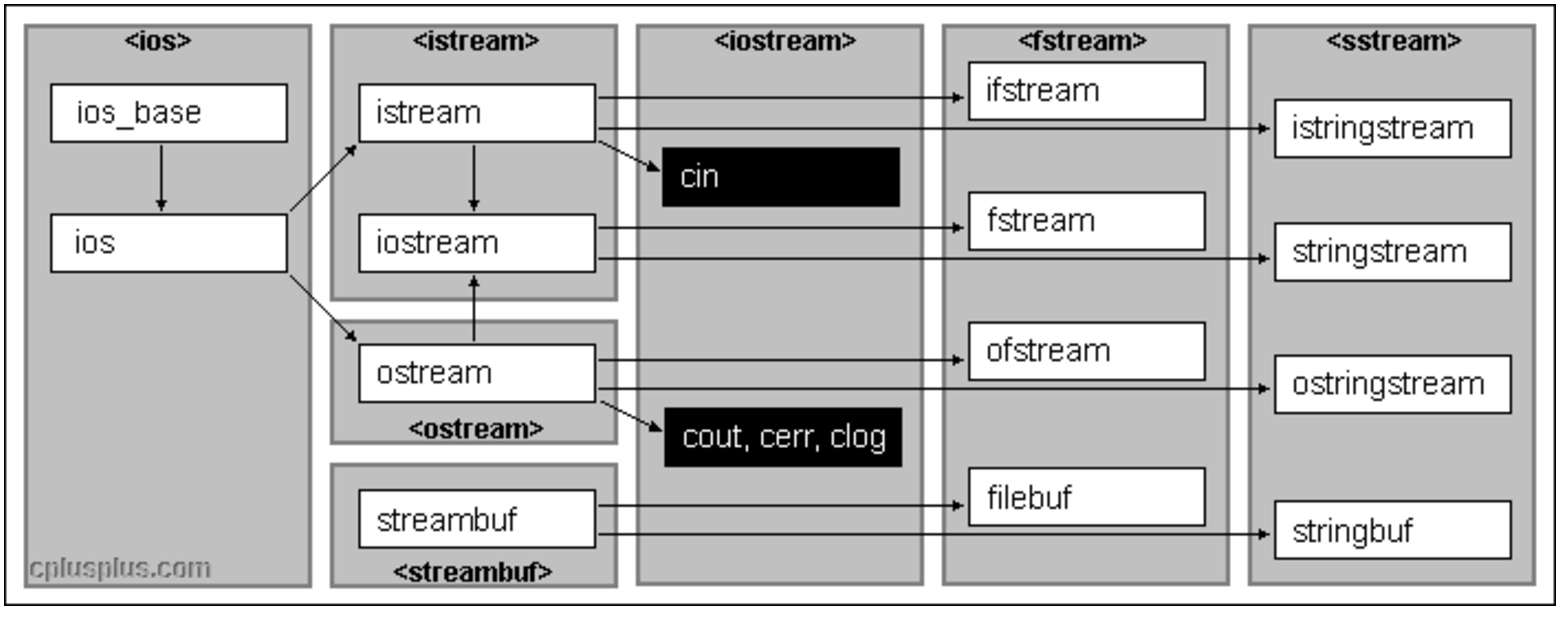
\includegraphics[scale=0.45]{pics/io.png}
\begin{enumerate}


\item \textbf{iofs} stand for three head files <iostream> <fstream> and <sstream>. <iostream> includes <ios> automatically. They are three main header file you should includes in your C++ application.

\item three classes: iostream(streambuf), fstream(filebuf), stringstream(stringbuf)

\item clog is just like cerr, but it buffer it output.

\item C++ normally flushes the input buffer when you press enter. For output to the display, C++ program normally flushes the output buffer when you transmit a newline character, or reaches an input statement.

\item \verb=>>= and \verb=<<= don't need to format string,  C++ will automatically,  convert it, it's better than printf and scanf in C language.

\item through inheritance, fstream and cin(cout) share the same usage. \textbf{All the knowledge can be used directly in fstream.} I like it the most.

\end{enumerate}

\end{itemize}


\subsubsection{Input basic knowledge}

\begin{itemize}
\item For Input, you need to master \textbf{One basic idea, Two languages, Three data type.}
\item One basic idea: In order to make continuously input, you need to use while(inputMethod), When two things happens:
\begin{enumerate}
\item user want to end input(ctrl+D) or read the end of File;
\item read fail (for example,  cin\verb=>>= int, but input letter 'a'),
\end{enumerate}

InputMethod will return false.  Then you need use some flag or status to tell the difference between EOF or error inside of while loop.

\item Two languages is c and c++, they use the different inputMethod. three data types are: number and word(no space in middle), character(white), and string(include space in middle)

\item two languages common used input method \\
\begin{tabular}{|p{0.08\textwidth}|p{0.27\textwidth}|p{0.3\textwidth}|p{0.3\textwidth}|}
\hline
& Number and non-white  character word & Character (including white-character) & string(line)\\
\hline
C &scanf("\%d \%f \%c \%s",\&i, \&f,\&c);  & int a = getchar(); & fgets(stdin, char*p, n ) \\
\hline
C++ & cin>>i>>f>>c>>w; & cin.get(char \& c); \newline  Ch = cin.get(); & cin.get( char *p, n); \newline cin.getline(char *p, n); \newline getline(cin, string);
 \\
\hline
\end{tabular}


\item In scanf, You need to specify exact data type when you read.
\begin{enumerate}
\item h:  short int or short unsigned. Example: \%hd or \%hu.

\item l:  a long int or long unsigned, or double (for \%f conversions.) Example: \%ld, \%lu, or \%lf.

\item L: The value to be parsed is a long long for integer types or long double for float types. Example: \%Ld, \%Lu, or \%Lf.

\item *: Tells scanf() do to the conversion specified, but not store it anywhere. This is what you use if you want scanf() to eat some data but you don't want to store it anywhere; you don't give scanf() an argument for this conversion. Example: \%*d.
\end{enumerate}


\item scanf("\%c" \&c) will read any character, including whitespace character. If you want to scanf skip any whitespace, you can use space before \%c.

\begin{lstlisting}[frame=single, language=c++, mathescape=true]
while(true){
  scanf("%c",&c);
  //scanf("$\Hilight{1}$ %c",&c);
  printf("you input: %d" c);
}
// When you input a(enter)
//output will be like
you input: 97(a value)
you input: 10(enter value)
\end{lstlisting}


\item cin\verb=>>=c will not read white character(tab, space , newline), If you want to read them from input buffer, You should use getchar() or cin.get(); If you want the user to input his or her name
\begin{lstlisting}[frame=single, language=c++, mathescape=true]
while(true){
  cin>>c;
  cout<<"you input:"<<c<<endl;
}
// When you input  "    a(enter)"
//output will be like
you input:  a
then cursor wait for here.
\end{lstlisting}

\item Using cin\verb=>>= or scanf will terminate the string after it reads the first space. The best way to handle this situation is to use the function to read a line;

\item Read word and line:
\begin{lstlisting}[frame=single, language=c++]
//read a word until reach white character.
Scanf(%s,char_array) //c
Cin>>char_array or ; //c++
Cin>> str;

//line	
gets(char_array)  //c
fgets(char_array, n , FILE *) //recommend to use this for safety.

cin.getline(char * ,int n) //c++ read and discard newline
cin.get(char * ,int n) //not read newline
std::getline(istream&  is, string& str)
\end{lstlisting}

\item cin.read function has the same interface with cin.get, but it doesn't append a null character to input, It's not intend for keyboard input, but for binary format of file

\item \textbf{For C++, three get, two getline, other use >>};

\item Difference between cin.get(char) and int = cin.get()
\begin{lstlisting}[frame=single, language=c++]
while(cin.get(c))
// use cin.get(char) in reading loop

cin.get() != '\n'
//use cin.get() return character to test sth.

cin.get()!= EOF
//When used in EOF, you have to use int
//because EOF may not be expressed by char tyep
\end{lstlisting}

\item Three confused functions: cin.get and cin.getline are almost the same thing.
\begin{lstlisting}[frame=single, language=c++]
cin.get ( char* s, streamsize n, char delim );
cin.getline (char* s, streamsize n, char delim );
istream& getline (istream&  is, string& str);
\end{lstlisting}

\begin{enumerate}

\item For each line, if you don't know the max length, juse use getline(cin, string). You don't need to input any length.(you can reserve lengh of string if you want to avoid allocation of memory)

\item cin.get() doesn't discard delim from input stream. However, cin.getline() will read and discard newline.  (It's easy for you to remember, because, \textbf{line} is defined by newline character)

\item In cin.getline(char* s, int n)The failbit flag is set if the function extracts no characters(newline is a character), Or if the delimiting character is not found once (n-1) characters have already been written to s. Note that if the character that follows those (n-1) characters in the input sequence is precisely the delimiting character, it is also extracted and the failbit flag is not set.

\item In cin.get(char* s ,  int n). The failbit flag is set only if the function extracts no characters.

\item If you are talking about the newline character from a console input,it makes perfectly sense to discard it, So use cin.getline(). Or you don't want to customized flexible reading method, just read a line from a file. please use cin.getline().

\item cin.get(char* s, n) is more flexible than cin.getline. Because when it read to the array is full, It doesn't set failbit. At this time you can use gcount() or peek() to see if next character is new line. It's more customized than  cin.getline();
\end{enumerate}

\end{itemize}

\subsubsection{custom stream}
\begin{enumerate}
\item \textbf{peek} return the next character from input without extracting from the input stream. For example, you want to read input up to the first newline or period.
\begin{lstlisting}[frame=single, language=c++]
char input[80];
int i = 0;
while( (ch=cin.peek()) != '.' && ch != '\n')
   cin.get(input[i++];)
input[i] = '\0';
\end{lstlisting}

\item \textbf{gcount()} method returns the number of characters read by the last unfromatted extraction method. That means character read by the a get(), getline(), ignore(), or read(), but not extraction operator.

\item \textbf{putback()} function inserts a character back in the input buffer.
\end{enumerate}


\subsubsection{Input error}

\begin{itemize}
\item \textbf{For the error of input: Just remember C language return EOF and NULL, and C++ return all false. }

 \begin{tabular}{|c|c|c|c|}
 \hline
  & Number, non-white & character, white  & string \\
 \hline
 C & scanf return EOF & getchar return EOF & fgets return NULL \\
 \hline
 c++ & cin return false & cin return false & cin.getline return false \\
 \hline
 \end{tabular}

 \item When you can't continue input, you need to know if it's end of file or fail. In C language, you can use feof and ferror function, in C++, you can use cin.eof(), cin.fail() or cin.bad() three functions. cin.bad() means serious system error happens, and input buffer can't be consistent and can't be recoveried anymore.

 \item When failbit or badbit are set. fail() return false, So you need to judge it by bad() again if this information is important for you.  Usually, bad() is not use very often.

\item eofbit is interesting topic. when you reach(not read) the "logical end-of-file", it will not be set, \textbf{It's set by a read function, not by position}   Instead,  You can use std::ifstream::peek() to check for the "logical end-of-file".

 \item \textbf{eof is set by last read EOF position} When you read EOF position, failbit is set and eof is set too. So If EOF is set, failbit must set too.  If only failbit is set, it means that input error happen.  Under these two conditions, istream will return false by operator bool.

\item In http://en.cppreference.com/w/cpp/io/basic\_ios/operator\_bool . You can see eofbit are true and failbit are false, operator bool return true. I don't' know when it will happen. \textbf{ eof() function returns "true" after the program attempts to read past the end of the file.}  But when read action set eofbit, it will set failbit at the sametime, so bool operator will return false because failbit are set.

\item How do you know if you read an incorrect input word, or if you are at the end of the file? This is when you use cin.eof() or feof() in C language.


\item you can use clear() and setstate() to set the states, Why? It's just depends on what the program is trying to accomplish.  It provides a means for you to change the state. setstate() is different with clear(), clear() clear all the status bit. but setstate just set specific bit.

\item You can use exceptions() method to control if exceptions will throw, when the eofbit, failbit and badbit is set.

\item setstate() is to provide a means for input and output functions to change the state. For end user, we don't use it very often. We just use clear() more.

 \item for rdstate() it will return all the bit value, then you can use \& to certain bit( such as failbit) to check if the bit has been set. But here, you can use fail() directly, so we don't use this function very often.
 \begin{lstlisting}[frame=single, language=c++]
std::ifstream is;
 is.open ("test.txt");
 if ( (is.rdstate() & std::ifstream::failbit ) != 0 )
    std::cerr << "Error opening 'test.txt'\n";
\end{lstlisting}


\item \textbf{clear() function is very important, when cin.fail() return true, you have to use clear(), otherwise all he below cin operation will not work.} See below example.

 \begin{lstlisting}[frame=single, language=c++]
char ch, str[20];
cin.getline(str, 5);
cout<<"flag1:"<<cin.good()<<endl;    // check good bit
cin.clear();   //without, cin>>ch below will not work at all
cout<<"flag1:"<<cin.good()<<endl;    // check good bit again
cin>>ch;
cout<<"str:"<<str<< " ch:" <<ch<<endl;

input:
12345[Enter]
output:
flag1:0 // good()return false
flag2:1 // good()return true after clear().
str:1234 ch:5
 \end{lstlisting}




\end{itemize}

\subsubsection{Input Pattern}

\begin{itemize}
\item It is bad idea to test the stream on the outside and then read/write to it inside the body of the conditional/loop statement. This is because the act of reading may make the stream bad. It is usually better to do the read as part of the test.

 \begin{lstlisting}[frame=single, language=c++]
while(!cin.fail()){  // that is bad programming style
    cin>>i;  //here may make stream fail().
    .....      //then i is not valid value
}
 \end{lstlisting}

\item If you just want to input, You don't want to know eof or deal with failbit. You can use below: \\

 \begin{lstlisting}[frame=single, language=c++]
while(scanf("%d",&i) != 1)
while((int c = getchar())!=EOF)
while( fgets(line, sizeof(line), fp) != NULL )
//in c language, use these to exit loop!

while(cin>>input)
while(cin.get(p, 20) )
while(getline(ifstream, string)) {
//in C++ language, use bool operator to exit loop.
  //do some useful things.  //input is right.
}
\end{lstlisting}

\item If you want to know eof or deal with error. You can use below:
\begin{lstlisting}[frame=single, language=c++]
While(true)  // use break to exit loop;
{
  cin>>i // or getline(ifstream, string);
  If(cin.eof()){   //If it's EOF
     cout<<"EOF encountered"<<endl
     break;
  }
  If(cin.fail())          //Invalide input
  {
     cin.clear();    //Important. clear state and buffer
     while(cin.get()!='\n')  //get rid rest of line,
               continue ;
       cout<<"please input a number"<<endl;
       continue;
  }
  ...  //do some useful things.  //input is right.
}
\end{lstlisting}




\item In the previous example, Why do we need to distinguish eof and fail? When fail happen, maybe there are invalid character in buffer. After clean the buffer, I can continue to read input from input buffer. Three methods to clean invalid character in the buffer
\begin{lstlisting}[frame=single, language=c++]
cin.clear();    //Important. clear state and buffer
while(cin.get()!='\n')
      continue ;      // method 1

while(!issapce(cin.get()))
            continue;  //method 2

basic_istream& ignore(streamsize _Count = 1, \
int_type _Delim = traits_type::eof());  //method 3
cin.ignore(5, 'a');
cin.ignore(numeric_limits<streamsize>::max(), '\n');
\end{lstlisting}

\item You can use istream\_iterator, It can save you some trouble to judge EOF.

\begin{lstlisting}[frame=single, language=c++]
#include <iostream>
#include <vector>
#include <algorithm>
#include <iterator>
using namespace std;
class A{
private:
int x;
int y;
friend istream& operator>>(istream& in, A&);
friend ostream& operator<<(ostream& in, const A&);
};

istream& operator>>(istream& in, A& a){
in>>a.x>>a.y;
return in;
}


ostream& operator<<(ostream& out, const A& a){
out<<a.x<< " " <<a.y;
return out;
}

int main(){
vector<A> v;
copy(istream_iterator<A>(cin), istream_iterator<A>(),
                                             back_inserter(v));
copy(v.begin(), v.end(),ostream_iterator<A>(cout, "\n"));
}

\end{lstlisting}


\item \textbf{In summary, It's better just use judgment to exit end loop.  If you need to different specific action to take to deal with EOF or error. Use while(true), then use eof() of feof() fail() or clear() functions in c++ and c to deal with and break the loop; }

\end{itemize}


\subsubsection{Output}
\begin{itemize}
\item For cout, It can recognize type automatically, and It is extensible, You can redefine \verb=<<= operator so that cout can recognize you data type.
\begin{lstlisting}[frame=single, language=c++]
class Foo{
friend ostream & operator<<(ostream& s, const Foo &r);
}

ostream & operator<<(ostream& s, const Foo &r){
s<<Foo.a<<Foo.b<<endl;
}
\end{lstlisting}

\item  How to print pointer address?
\begin{lstlisting}[frame=single, language=c++]
char* amount = "dozen";
cout<< amount  ; //print "dozen" string

cout<<(void*) amount;   //prints the address of pointer
printf("%p", (void*) p);
\end{lstlisting}


\item Format is key point for Output. you need to know the common manipulator to control the output format.
\item Number base manipulators:  hex, oct  and dec; Field widths: Width,  fill, precision Setf()
\item You don't need to know the details, just name of them. When you want to use them go to reference website to look.A detail format manipulators can be seen on C++ primer P1090. You need to include <iomanip>

\item \verb=<<= is a bitwise left-shift operator in C language, but in C++, we overloaded it in ostream class, cout is a object of ostream,

\item You can use \verb=cout<<flush= to force flushing the output buffer
\item cout.write can be used to output a string, It will output certain length string, even reach the end of string.


\end{itemize}

\subsubsection{file}
\begin{itemize}
\item 	When you studied cin and cout very well, you will find that file operation is so easy. just change cin or cout to your ifstream , ofstream or fstream object.

\begin{lstlisting}[frame=single, language=c++]
std::fstream fs;
fs.open ("test.txt", ios_base::in| ios_base::binary);
if(!ifs.is_open())
     exit(1);
char c = ifs.get();
// use all previous input methods
ifs.close();
\end{lstlisting}


\item Only read ifsteam;  Only write ofsteam; write and read fstream.

\item For ios\_base::binary mode, use write() and read() funciton.

\item For writing, pay attention to the difference between ios\_base::trunc and ios\_base::app

\item Random access is used mostly on binary file. Because the position can be pinpointed exactly. For seekg() for input, and seekp() for output.(p is put, g is get) It move the pointer. tellp() and tellg() function.  It tell the position of pointer.

\end{itemize}

\subsubsection{buffer and string buffer}

\begin{itemize}


\item stringstream is a convenient way to manipulate strings like an independent I/O device .
Sometimes it is very convenient to use stringstream to convert bettween strings and other numerical types. The usage of stringstream are much the same with iostream, so it is not a burden to learn.  

\item \textbf{You need to build a stringstream from a string, or convert a stringstream back to a string.}

\begin{lstlisting}[frame=single, language=c++]
stringstream outstr;
//change number to a text
outstr<<"salary value"<<123333.00<<endl;
String str = outstr.str() //change to string

//change text to number
Istringstream Instr(str);
While(instr>>number)
cout<<number<<endl
////////below is C language/////////
char sentence []="Yan is 41 years old";
char str [20];
int i;
sscanf (sentence,"%s %*s %d", str, &i);
//* means input will be ignored. So str = Yan, i = 41.
sprintf(.....);
\end{lstlisting}

\end{itemize}

\subsection{efficiency}
\begin{itemize}
\item  lazy evaluation includes 1) reference counting (to avoid extra copy) 2) distinguish read from write 3) lazy fetching. 4) lazy expression evaluation. Detail see in "More Effective C++". Usually, implementation will be  more complex with lazy evaluation.

\end{itemize}


\section{pointer and smart pointer}

\subsection{function pointer}
\begin{itemize}

\item A real example of function pointer is set\_new\_handler. It accepts a function pointer and return the same function pointer, so declaring such format is a little difficult.
\begin{lstlisting}[frame=single, language=c++]
void failNew(){
cerr<<"Fail now"<<endl
abort();
}
-----------------------------------------
extern void ( *set_new_handler ( void (*)() ) ) ();
// This function declaration is very complex.
set_new_handler(failNew);
\end{lstlisting}

\item A better method is to use typedef method.

\begin{lstlisting}[frame=single, language=c++]
typedef void(* FunPtr)();

FunPtr (*set_new_handler) (FunPtr);

set_new_handler(failNew);
\end{lstlisting}

\item in C++ 11, When you want a function pointer, encourage you to use more lambda idiom. You also can use \texttt{auto} to store a lambda function for future use.
\end{itemize}

\subsection{When to use new?}
\begin{itemize}

\item When do you use smart pointer? Here I change this questions to another question, When do you use pointer?
\begin{enumerate}

\item An new object remain in existence, until you delete it. (you control the life time of it, maybe you create it in fun1,then delete it in fun4. so the obj is neither stack life nor global life. You may or may not transfer \textbf{ownership} between functions.)

\item When you want to create a obj in runtime according runtime condition or user input dynamically. (maybe don't create it. ) Below code demonstrates previous two conditions.  \texttt{ToothBrush} need to be control life time and created dynamically.

\begin{lstlisting}[frame=single, language=c++]
class Person{
ToothBrush* pbrush;

buyNewBrush(string &name){
    if(pbrush != nullptr}{
	    	delete pbrush;
    }
    if(name == "Orlab")
          pbrush = new Brush();
    }
}
~Person(){
	if(pbrush != nullptr}{
		delete pbrush;
    }
}
///////////////////
Person Yan();
Yan.buyNewBrush("Oralb");
......Three months later...........
Yan.buyNewBrush("Philip");
}
\end{lstlisting}

\item Large array or resources,  if you allocate in stack, it will cause stack overflow. \textbf{In practices, this requirement is deprecated, because any time when you use [] or new [], you need consider to use array or vector ans string!}
\end{enumerate}

\item \textbf{Never say new in c++14!} 
\end{itemize}


\subsection{Smart pointer Basic knowledge}

\begin{itemize}
\item A simple auto\_ptr source code: You can learn how to overload operator*() and operator->().
\begin{lstlisting}[frame=single, language=c++, mathescape=true]
template <class T> class auto_ptr{
    T* ptr;
public:
    explicit auto_ptr(T* p = 0) : ptr(p) {}
    ~auto_ptr()                 {delete ptr;}
    $\Hilight{12}$T& operator*()     {return *ptr;}
    $\Hilight{12}$T* operator->()    {return ptr;}
    // ...
};

auto_ptr<int> aupr;
//aupr is nullptr even you don't initialize it.
\end{lstlisting}

\item Why do we need smart pointer?
\begin{enumerate}
\item "Just remember" is seldom the best solution! So we need smart pointer to perform delete operator automatically.

\item When throw an exception, or return in the middle of code. delete will not be invoked at all, It will cause memory leaking. When you use smart pointer, If an exception is thrown in the middle of fun, there will no be memory leak.
\begin{lstlisting}[frame=single, language=c++]
void methodA() {
   unique_ptr<int> buf(new int[256]);

   int result = fillBuf(buf))
   if(result == -1)
      return;
}
\end{lstlisting}

\item smart pointer is nullptr default if you don't initialize. You avoid wild pointer problem.

\item \textbf{smart pointer can manage exclusive ownership or shared ownership automatically. }
\end{enumerate}

\item There are four kinds of smart pointer: \texttt{auto\_ptr} \texttt{unique\_ptr} \texttt{shared\_ptr} and \texttt{weak\_ptr}  But only \texttt{unique\_ptr} , \texttt{shared\_ptr} and \texttt{weak\_ptr} are recommended to use. auto\_ptr is now deprecated, and should not be used in new code. When you get a chance, try doing a global search-and-replace of auto\_ptr to unique\_ptr in your code base. weak\_ptr is mainly used for observer, you can always use raw pointer or reference for this purpose. Raw pointer can't check if pointee object is still valid, weak\_ptr can accomplish this task.

\item Why auto\_ptr not recommended? 1) When you assign targetP = sourceP, it will cause sourceP set to be NULL, It will cause trouble when you use sourceP in the future.  2)You can't create container includes auto\_ptr, compiler prohibit you doing so!
\begin{lstlisting}[frame=single, language=c++]
auto_ptr<string> ps (new string("hello world") );
auto_ptr<string> ps1;
ps1 = ps;   // ps will be set null.
ps->size() // it will crash the application.

auto_ptr<string> parray[5]; //compiling error.
auto_ptr<string> ps = parray[2];
//parray[2] will be set null;
\end{lstlisting}

\item \textbf{When you construct a smart pointer, you must use 1) a pointer and 2) this pointer must be produced by new.} You can't build smart pointer by address operator. such as unique\_ptr<double> ptr(\&int);   Why? because smart pointer will call delete when it is out of scope.  delete operator has to be used on pointer produced by new operator.

\item Obtain the raw pointer (get), to relinquish control of the pointed object (release), and to replace the object it manages (reset).
\begin{lstlisting}[frame=single, language=c++]
string * cp = new string("hello world");
shared_ptr<string> ps(cp);
string * cp1 = ps.get(); //use get() get normal pointer.
\end{lstlisting}


\item Smart pointer has bool operator, you can use if to test if it's nullptr directly.
\begin{lstlisting}[frame=single, language=c++]
 std::unique_ptr<int> ptr(new int(42));
 if (ptr) std::cout <<  *ptr << '\n';
 ptr.reset();
 if (ptr) std::cout <<  *ptr << '\n';
\end{lstlisting}

\item Smart pointer and const:
\begin{lstlisting}[frame=single, language=c++]
shared_ptr<T> p;        ---> T * p;
const shared_ptr<T> p;   ---> T * const p;
shared_ptr<const T> p;   ---> const T * p;
const shared_ptr<const T> p; ---> const T * const p;
\end{lstlisting}

\end{itemize}

\subsection{unique\_ptr}

\subsubsection{basic}
\begin{itemize}

\item unique\_ptr basic 1-1: create unique\_ptr from new.    \textbf{make\_unique is better than inside new, inside new is better than outside new.}
\begin{lstlisting}[frame=single, language=c++]
string * cp = new string("hello world");

unique_ptr<string> ps = cp; /$\Hilight{8}$/ NOT allow

//ok, but not good style(outside new)
unique_ptr<string> ps (cp);

//good style(inside new)
unique_ptr<string> ps (new string("hello world"));

//best style make_unique
unique_ptr<string> ps( std::make_unique<string>("hello") );
\end{lstlisting}

\item unique\_ptr basic 1-2: Create unique\_ptr from another unique\_ptr, you have to use move.
\begin{lstlisting}[frame=single, language=c++]
unique_ptr<string> ps1 (new string("hello world"));

unique_ptr<string> ps2 ( ps1 ); //compile error, not allow.
unique_ptr<string> ps2 ( move(ps1) ); //ok
//ownship transfer from ps1 to ps2, nothing delete.
\end{lstlisting}

\item \texttt{unique\_ptr} basic 2: When pass value into a function, \textbf{1) for some exist \texttt{unique\_ptr}, use move to transfer ownership, 2) for new \texttt{unique\_ptr}, use \texttt{make\_unique} to assure exception safe.}

\begin{lstlisting}[frame=single, language=c++]
void sink( unique_ptr<widget> arg1, unique_ptr<gadget> arg2);

//1) use move
sink( std::move(exist_uptr_wi), std::move(exist_uptr_ga))

//2) use make function to assure exception safety.
sink( make_unique<widget>(new ...),
make_unique<gadget>(new ...) );  // exception-safe
\end{lstlisting}


\item unique\_ptr basic 3: unique\_ptr assignment
\begin{lstlisting}[frame=single, language=c++]
unique_ptr<string> ps1 (new string("ps1"));
unique_ptr<string> ps2 (new string("ps2"));

ps1= ps2; //compile error, not allow

//method1: use move
ps1 = std::move(ps2);
//pointer inside previous ps1 will be deleted.
// pointer inside ps1 point to "ps2" string now.
//pointer inside ps2 will set to null

//method2: reset
ps1.reset(cp); //ok
//pointer inside previous ps1 will be delete

string* pstr = ps1.release();
// use pstr get pointer managed by ps1.
\end{lstlisting}

\item unique\_ptr basic 4-1: If a program attempts to assign one unique\_ptr to another. The compiler allows it if the source object is a temporary rvalue (It will call move ctor or assignment of unique\_ptr inside.) and disallows it if the source object has some duration. \textbf{It is a move-only type.}
\begin{lstlisting}[frame=single, language=c++, mathescape=true]
unique_ptr<string> ps2 = $\Hilight{19}$uqique_ptr<string>(new string("yo") ); //OK

uqique_ptr<string> fun(){
return unique_ptr<string> temp(new string("yan");
}
pu2 = fun(); //OK
\end{lstlisting}

\item unique\_ptr basic 4-2: unique\_ptr support source and sink idiom.
\begin{lstlisting}[frame=single, language=c++]
unique_ptr fun() //support source

fun(unique_ptr up);  //use move to support sink
fun(move(other_up));
\end{lstlisting}

\item unique\_ptr basic 5: Just observer, not transfer ownership , you can get pointer, or use unique\_ptr reference.
\begin{lstlisting}[frame=single, language=c++]
unique_ptr<string> ps1 (new string("ps1"));

fun(string* pstr);
fun(unique_ptr<string> & ref_ptr);
\end{lstlisting}

\item by default, std::unique\_ptrs are the same size as raw pointers, so efficiency of it is just like raw pointer.

\item Unique\_ptr has new [] version. The existence of std::unique\_ptr for arrays should be of only intellectual interest to you, because std::array, std::vector, and std::string are virtually always better data structure choices than raw arrays. About the only situation I can conceive of when a std::unique\_ptr<T[]> would make sense would be when you're using a C-like API that returns a raw pointer to a heap array that you assume ownership of it.
\begin{lstlisting}[frame=single, language=c++]
unique_ptr<double []>  pda(new double[5] );
// it will call delete [] inside.
\end{lstlisting}

\item When in doubt, prefer unique\_ptr by default, and you can always later move-convert to shared\_ptr if you need it. If you do know from the start you need shared ownership, however, go directly to shared\_ptr via make\_shared. If you compiler report error about unique\_ptr, then you should consider to use shared\_ptr

\item unique\_ptr can be used inside of class. Below class B disable value-copying (or to define a suitable copy-constructor  and operator= to handle it safely).
\begin{lstlisting}[frame=single, language=c++]
class B {  // this class can't be copy
public:
   unique_ptr<int> i;
   B():i(new int(0)) { }
};
\end{lstlisting}
\item A common use for std::unique\_ptr is as a factory function return type for objects
in a hierarchy. Detail can be seen "effective modern c++ item 18"

\begin{enumerate}
\item During construction, std::unique\_ptr objects can be configured to use custom deleters: arbitrary functions (or function objects, including those arising from lambda expressions) to be invoked when it's time for their resources to be destroyed. when a custom deleter can be implemented as either a function or a captureless lambda expression, the lambda is preferable.

\item When a custom deleter is to be used, its type must be specified as the second type argument to std::unique\_ptr.
\end{enumerate}

\begin{lstlisting}[frame=single, language=c++, mathescape=true]
//only c++ 14 support return type deduction
template<typename... Ts>
$\Hilight{4}$auto makeInvestment(Ts&&... params) {
auto delInvmt = [](Investment* pInvestment) {
makeLogEntry(pInvestment); // makedelete
delete pInvestment; // Investment
};

std::unique_ptr<Investment, decltype(delInvmt)>
pInv(nullptr, delInvmt);

if (...){
pInv.reset(new Stock($\Hilight{16}$std::forward<Ts>(params)...));
}
else if (... ) {
pInv.reset(new Bond(std::forward<Ts>(params)...));
}
return pInv; // as before
}
\end{lstlisting}

\item std::unique\_ptr is the C++11 way to express exclusive ownership, but one of its
most attractive features is that it easily and efficiently converts to a std::shared\_ptr: This is a key part of why std::unique\_ptr is so well suited as a factory function return type. Factory functions can't know whether callers will want to use exclusive ownership semantics for the object they return or whether shared ownership
\begin{lstlisting}[frame=single, language=c++, mathescape=true]
std::shared_ptr<Investment> sp = // converts std::unique_ptr
makeInvestment( arguments ); // to std::shared_ptr
\end{lstlisting}

\end{itemize}

\subsubsection{unique\_ptr and container}
\begin{itemize}

\item If your vector should hold std::unique\_ptr<Fruit> instead of raw pointers (to prevent memory leaks). vector need copy in and copy out. but unique\_ptr don't support copy. So 1) you can use emplace\_back with new pointer, but it will lead memory leak if extending vector size fail. 2) use unname unique\_ptr, 3) use make\_unique .
\begin{lstlisting}[frame=single, language=c++]
class Fruit { ... };
class Pear : Fruit { ... };
class Tomato : Fruit { ... };

std::vector<std::unique_ptr<Fruit> > m_fruits;
//method 1, bad
m_fruits.emplace_back(new Pear);

//method 2, good
m_fruits.push_back(std::unique_ptr<Fruit>(new Pear));
m_fruits.push_back(std::unique_ptr<Fruit>(new Tomato));

//method 3, best using std::make_unique:
m_fruits.push_back(std::make_unique<Pear>());
m_fruits.push_back(std::make_unique<Tomato>());
\end{lstlisting}

\item You can store unique\_ptr objects in an STL container providing you don't invoke methods or algorithm, such as copy(), that copy or assign one unique\_ptr to another.  see effective stl item 8.

\begin{lstlisting}[frame=single, language=c++]
bool compare_by_uniqptr(
               const unique_ptr<SomeLargeData>& a,
               const unique_ptr<SomeLargeData>& b) {
    return a->id < b->id;
}

sort(vec_byuniqptr.begin(), vec_byuniqptr.end(),
compare_by_uniqptr);
\end{lstlisting}


\begin{lstlisting}[frame=single, language=c++]
typedef std::unique_ptr<int> unique_t;
typedef std::vector< unique_t > vector_t;

vector_t vec2(5, unique_t(new Foo));     // Error (Copy)
vector_t vec3(vec1.begin(), vec1.end()); // Error (Copy)
std::copy(vec1.begin(), vec1.end(),
          std::back_inserter(vec2)); // Error (copy)

vector_t vec3(make_move_iterator(vec1.begin()),
                 make_move_iterator(vec1.end())); //Ok

std::sort(vec1.begin(), vec1.end());
// OK, because using Move Assignment Operator
\end{lstlisting}

\end{itemize}




\subsection{shared\_ptr}
\begin{itemize}

\item shared\_ptr basic 1: create shared\_ptr from new. \textbf{make\_shared is better than inside new, inside new is better than outside new.}
\begin{lstlisting}[frame=single, language=c++]
string * cp = new string("hello world");

shared_ptr<string> ps = cp; // $\Hilight{8}$NOT allow

//method1: use constructor
shared_ptr<string> ps (cp); //ok, but not good style
shared_ptr<string> ps (new string("hello world")); //good style

//method2: make_shared function
unique_ptr<string> ps( std::make_shared<string>("hello world") );
\end{lstlisting}

\item shared\_ptr basic 1-1: First, try to avoid passing raw pointers to a std::shared\_ptr constructor. 1) use make\_share(). 2) if you have custom deleter and can't use make\_share().  Pass the result of new directly instead of going through a raw pointer variable.

\begin{lstlisting}[frame=single, language=c++]
auto pw = new Widget; // pw is raw ptr

std::shared_ptr<Widget> spw1(pw, loggingDel);
// create control block for *pw
std::shared_ptr<Widget> spw2(pw, loggingDel);
// create 2nd control block for *pw!
//$\Hilight{20}$ BAD! That will cause undefine result!
\end{lstlisting}

\item shared\_ptr basic 2: Create shared\_ptr from another shared\_ptr
\begin{lstlisting}[frame=single, language=c++, mathescape=true]
shared_ptr<string> ps1 (new string("hello world"));

shared_ptr<string> ps2 ( ps1 );
//use_count of ps1 and ps2 are all 2

shared_ptr<string> ps2 ( move(ps1) );
//the original ps1 will become null, and
//the reference count does not get modified.
$\Hilight{20}$//Just transfer use_count to ps2. 
\end{lstlisting}

\item shared\_ptr basic 3: shared\_ptr assignment
\begin{lstlisting}[frame=single, language=c++, mathescape=true]
shared_ptr<string> ps1 (new string("ps1"));
shared_ptr<string> ps2 (new string("ps2"));

//method1: use assignment
ps1 = ps2;
$\Hilight{9}$// 1) previous use_count decrements 1(If equal 0, will delete)
$\Hilight{9}$// 2) ps1 points to current use_count
$\Hilight{9}$// 3) and current use_count increments 1

//method2: use move
ps1 = std::move(ps2);
$\Hilight{9}$// 1) previous use_count decrements 1(If equal 0, will delete)
$\Hilight{9}$// 2) ps1 points to current use_count
$\Hilight{9}$// 3) ps2 is null now. 


//method3: reset
ps1.reset(cp); //ok
//pointer inside previous ps1 will decrement 1.
//by now, current ps1 reference count will be 1.
\end{lstlisting}

\item shared\_ptr basic 4: Difference between ctor and assignment.
\begin{enumerate}
\item When assignment, previous decrements 1 and current increment 1;
\item When copy ctor, current increment 1;
\item When ctor from raw pointer, current is 1;
\end{enumerate}

\item shared\_ptr basic 5: Just observer, not transfer ownership , you can get pointer, or use shared\_ptr reference. Or use reference directly!
\begin{lstlisting}[frame=single, language=c++]
shared_ptr<string> ps1 (new string("ps1"));

fun(string* pstr);
fun(shared_ptr<string> & ref_ptr);
\end{lstlisting}

\item inside of shared\_ptr: \newline
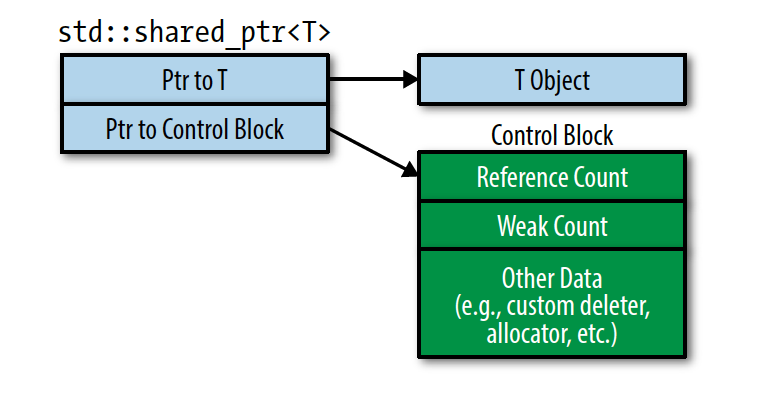
\includegraphics[scale=0.8]{pics/shared.png}

\item \textbf{When are control blocks created?}  It's very important conception, when you understand it, you will know what happen when you create or assign a shared\_ptr better. 
		
\begin{enumerate}
\item std::make\_shared  always creates a control block. It manufactures
a new object to point to, so there is certainly no control block for that
object at the time std::make\_shared is called.

\item A control block is created when a std::shared\_ptr is constructed from a
unique-ownership pointer (i.e., a std::unique\_ptr ). As part of its construction, the std::shared\_ptr assumes ownership of the pointed-to object, so the uniqueownership pointer is set to null.

\item When a std::shared\_ptr constructor is called with a raw pointer, it creates a control block.

\item std::shared\_ptr constructors taking std::shared\_ptrs or std::weak\_ptrs as constructor arguments. \textbf{NOT} create new control blocks, because they can rely on the smart pointers passed to them to point to any necessary control blocks

\end{enumerate}


\item Like std::unique\_ptr, std::shared\_ptr uses delete as its default resource-destruction mechanism, but it also supports custom deleters.
\begin{lstlisting}[frame=single, language=c++]
std::unique_ptr< Widget, decltype(loggingDel) >
                               upw(new Widget, loggingDel);
// deleter type is ptr type

std::shared_ptr<Widget> spw(new Widget, loggingDel);
 // deleter type is not part of ptr type
\end{lstlisting}

\item In order to correctly use shared\_ptr with an array, you must supply a custom deleter. But we don't recommend using shared\_ptr with array. \textbf{Any time you new a array, you should first consider using STL container directly.}
\begin{lstlisting}[frame=single, language=c++]
template< typename T >
struct array_deleter {
  void operator ()( T const * p){
    delete[] p;
  }
};

std::shared_ptr<int> sp( new int[10], array_deleter<int>() );
\end{lstlisting}

\item usage of enable\_shared\_from
\begin{lstlisting}[frame=single, language=c++]
#include <iostream>
#include <boost/enable_shared_from_this.hpp>
#include <boost/shared_ptr.hpp>
class Test : public boost::enable_shared_from_this<Test>        //改进1
{
public:
    
    ~Test() { std::cout << "Test Destructor." << std::endl; }
    boost::shared_ptr<Test> GetObject()
    {
        return shared_from_this();      //改进2
    }
};
int main(int argc, char *argv[]){
        boost::shared_ptr<Test> p( new Test( ));
        boost::shared_ptr<Test> q = p->GetObject();
    
    return 0;
}
\end{lstlisting}


\end{itemize}

\subsection{wrapping resource handler in smart pointer}

\begin{itemize}
\item There are two different resource handlers: One is window api return value, The other is FILE* in C language

\item Example for FILE* is below:

\begin{lstlisting}[frame=single, language=c++]
unique_ptr<std::FILE, decltype(&std::fclose)> 
                   fp(std::fopen("demo.txt", "r"), &std::fclose);
if(fp) // fopen could have failed; in which case fp holds a null pointer
\end{lstlisting}

\item We can make FILE* example better, use unique\_ptr source semantic.
\begin{lstlisting}[frame=single, language=c++]
struct FILEDeleter {
    void operator()(FILE *pFile){
        if (pFile)
            fclose(pFile);
    }
};

using FILE_unique_ptr = unique_ptr<FILE, FILEDeleter>;

FILE_unique_ptr make_fopen(const char* fname, const char* mode){
    FILE *fileHandle= nullptr;
    auto err = fopen_s(&fileHandle , fname, mode); 
    if (err != 0){
        // print info, handle error if needed...
        return nullptr;
    }
    return FILE_unique_ptr(fileHandle);
}

//usage in your code!
FILE_unique_ptr pInputFilePtr = make_fopen("test.txt", "rb");
if (!pInputFilePtr)
    return false;
\end{lstlisting}

\item If you want to use shared\_ptr wrap FILE*, see below example.
\begin{lstlisting}[frame=single, language=c++]
using FILE_shared_ptr = std::shared_ptr<FILE>;

FILE_shared_ptr make_fopen_shared(const char* fname, const char* mode){
    FILE *fileHandle = nullptr;
    auto err = fopen_s(&fileHandle, fname, mode);
    if (err != 0){
        // handle error if needed
        return nullptr;
    }

    return FILE_shared_ptr(fileHandle, $\Hilight{15}$FILEDeleter());
    //Pay attention!, Here we use FILEDeleter(), but unique_ptr use FILEDeleter
}
\end{lstlisting}

\item You should know \textbf{HANDLE in windows is just void* type pointer}, so you can use this way to deal with windows handle.

\begin{lstlisting}[frame=single, language=c++]
struct HANDLEDeleter{
    void operator()(HANDLE handle) const{
        if (handle != INVALID_HANDLE_VALUE)
            CloseHandle(handle);
    }
};

using HANDLE_unique_ptr = unique_ptr<void, HANDLEDeleter>;

HANDLE_unique_ptr make_HANDLE_unique_ptr(HANDLE handle){
    if (handle == INVALID_HANDLE_VALUE || handle == nullptr){
        // handle error...
        return nullptr;
    }
return HANDLE_unique_ptr(handle);
}

auto hInputFile = make_HANDLE_unique_ptr(CreateFile(strIn, GENERIC_READ, ...));
if (!hInputFile)
    return false;
\end{lstlisting}

\item In unique\_ptr type. std::remove\_reference<Deleter>::type::pointer if that type exists, otherwise T*. Must satisfy NullablePointer.

\item For unique\_ptr, if you can deduct pointer type from deleter, unique\_ptr will use it directly, so you just know SC\_HANDLE is pointer, but you don't know exact type, you can write just like below: 
\begin{lstlisting}[frame=single, language=c++]
struct SvcHandleDeleter{
    typedef SC_HANDLE pointer;
    SvcHandleDeleter() {};

    template<class Other> SvcHandleDeleter(const Other&) {};
    void operator()(pointer h) const {
        CloseServiceHandle(h);
    }
};

typedef std::unique_ptr<SC_HANDLE,SvcHandleDeleter> unique_sch;

unique_sch scm(::OpenSCManagerA(0, 0, SC_MANAGER_ALL_ACCESS));
\end{lstlisting}

\item For shared pointer, type-erasure makes it impossible with the current interface to achieve exactly what type you want. So you can use a dumb way, Just like a pointer to pointer. If you don't know what is behind SC\_HANDLE. If you know it's type is void, you can use void directly, it will save you a lot of trouble. 

\begin{lstlisting}[frame=single, language=c++]
std::shared_ptr<SC_HANDLE> sp(new SC_HANDLE(::OpenSCManagerA(0, 0, SC_MANAGER_ALL_ACCESS)),
    [](SC_HANDLE* p){ ::CloseServiceHandle(*p); delete p; });
\end{lstlisting}

\item A common example can be found here:
\begin{lstlisting}[frame=single, language=c++]
typedef struct {
    int m_int;
    double m_double;
} Foo;

Foo* createObject(int i_val, double d_val) {
    Foo* output = (Foo*)malloc(sizeof(Foo));

    output->m_int = i_val;
    output->m_double = d_val;

    puts("Foo created.");
    return output;
}

void destroy(Foo* obj) {
    free(obj);
    puts("Foo destroyed.");        
}

std::shared_ptr<Foo> foo(createObject(32, 3.14), destroy);
\end{lstlisting}

\begin{lstlisting}[frame=single, language=c++]
struct FooDeleter {
    void operator()(Foo* p) const {
        destroy(p);
    }
};
using FooWrapper = std::unique_ptr<Foo, FooDeleter>;
FooWrapper foo(createObject(32, 3.14));
\end{lstlisting}

\item Use shared\_ptr to wrap a handle, A good introduction is "Making a HANDLE RAII-compliant using shared\_ptr with a custom deleter" in stackoverflow


\item Sometimes, I want to keep file alive, because foo and bar will use them. You can't use RAII auto object. And If you use raw pointer, It's difficult to trace and delete it. shared\_ptr is the best options right now.  you don't needs to worry about deleting file - once both foo and bar have finished and no longer have any references to file (probably due to foo and bar being destroyed), file will automatically be deleted.

\begin{lstlisting}[frame=single, language=c++]
void setLog(const Foo & foo, const Bar & bar) {
//File file("/path/to/file", File::append);  1) //RAII auto obj
//File* file = new File("/path/to/file", File::append); //2) raw new
   shared_ptr<File> file =
              new File("/path/to/file", File::append); //3) best
              
   foo.setLogFile(file);
   bar.setLogFile(file);
}
\end{lstlisting}

\item for fstream, it's different with FILE*. It's based on value semantic. So common usage just fstream f1; f1.open and f1.close. If you want to manage it's time smartly, you can produce a fstream* pointer and wrapped by shared\_ptr. You can use FILE* if you don't mind using C language.

\item fstream is value semantic, so you can use shared\_ptr directly. just like to deal with other value semantic variable, such as int and class.
\begin{lstlisting}[frame=single, language=c++]
shared_ptr<fstream> fp{new fstream(name,mode)};
if(!*fp)
  throw No_file{};
ClassA a(fp);
ClassB b(fp);
\end{lstlisting}

\item The std::unique\_ptr template has two parameters: the type of the pointee, and the type of the deleter. This second parameter has a default value, so you usually just write something like std::unique\_ptr<int>.

The std::shared\_ptr template has only one parameter though: the type of the pointee. But you can use a custom deleter with this one too, even though the deleter type is not in the class template. The usual implementation uses type erasure techniques to do this.Is there a reason the same idea was not used for std::unique\_ptr?

Part of the reason is that shared\_ptr needs an explicit control block anyway for the ref count and sticking a deleter in isn't that big a deal on top. unique\_ptr however doesn't require any additional overhead, and adding it would be unpopular- it's supposed to be a zero-overhead class. unique\_ptr is supposed to be static.

You can always add your own type erasure on top if you want that behaviour- for example, you can have \texttt{unique\_ptr<T, std::function<void(T*)>>}, something that I have done in the past.

\item by now, shared\_ptr and std::functions use type erase technology. 

\end{itemize}


\subsection{weak\_ptr}
\begin{itemize}

\item The relationship begins at birth. std::weak\_ptrs are typically created from std::shared\_ptrs. You can only create a weak\_ptr out of a shared\_ptr or another weak\_ptr. So the idea would be that the owner of the pointer hold a shared\_ptr instead of a raw pointer.


\item std::weak\_ptrs can't be dereferenced, nor can they be tested for nullness. That's because std::weak\_ptr isn't a standalone smart pointer. It's an augmentation of std::shared\_ptr. Almost the only things you can do are to interrogate it to see if the managed object is still there, or construct a shared\_ptr from it.

\begin{lstlisting}[frame=single, language=c++,mathescape=true]
auto spw =
std::make_shared<Widget>();
// the pointed-to Widget's ref count (RC) is 1.

std::weak_ptr<Widget> wpw(spw);
// wpw points to same Widget as spw. RC remains 1
...
spw = nullptr;
// RC goes to 0, and the Widget is destroyed.
// wpw now dangles
$\Hilight{12}$if (wpw.expired())
// if wpw doesn't point to an object…
\end{lstlisting}

\begin{lstlisting}[frame=single, language=c++,mathescape=true]
std::shared_ptr<Widget> spw1 = wpw.lock();
// if wpw's expired, spw1 is null
auto spw2 = wpw.lock();
// same as above, but uses auto

std::shared_ptr<Widget> spw3(wpw);
// if wpw's expired, throw std::bad_weak_ptr
\end{lstlisting}


\item Potential use cases for std::weak\_ptr includes: caching, observer lists, and the prevention of std::shared\_ptr cycles.  All the detail can be seen in "Effective Modern ++" Item 20.
\begin{lstlisting}[frame=single, language=c++]
std::shared_ptr<const Widget> fastLoadWidget(WidgetID id)
{
static std::unordered_map<WidgetID,
std::weak_ptr<const Widget>> cache;
auto objPtr = cache[id].lock();
// objPtr is std::shared_ptr to cached object (or null
// if object's not in cache)
if (!objPtr) { // if not in cache,
objPtr = loadWidget(id); // load it
cache[id] = objPtr; // cache it
}
return objPtr;
}
\end{lstlisting}

\item For above requirement, you also can use raw pointer, But for raw pointer, you can't detect if original one has been delete. 

\item A truly smart pointer would deal with this problem by tracking
when it dangles, i.e., when the object it is supposed to point to no longer exists. That's precisely the kind of smart pointer std::weak\_ptr is. \textbf{You can't test if a raw pointer is dangle or not.}

\end{itemize}


\subsection{smart pointer and polymorphism}

\begin{itemize}
\item In this section, you need to know four things:
\begin{enumerate}
\item share\_ptr child to base;
\item share\_ptr base to chile (down cast);
\item unique\_ptr child to base;
\item unique\_ptr base to chile (down cast);
\end{enumerate}

		\item \textbf{Basic idea: smart pointer base and smart pointer are not covariant at all. You can think that just like vector<Base> and vector<derived>}.

		\item For shared\_ptr, it support derived to base shared\_ptr copy or assignment. Behind the hood, you need to know the template member function. Detail can be found in effective C++ item 45 "Use member function templates to accept "all compatible types". Why you can? because it get raw pointer and wrapped it again and compiler allow it.

		\item  For shared\_ptr base, you can't assign it to the shared\_ptr child, so you must use static\_pointer\_cast and dynamic\_pointer\_cast. 1) they only support shared\_ptr. 2) They use shared\_ptr aliasing ctor, get raw pointer, use static or dynamic cast, then build derived shared\_ptr too. Detail can be found "
std::static\_pointer\_cast vs static\_cast<std::shared\_ptr<A>>"

\item For shared\_ptr base reference, You have to use const. Why do we need const, 1) from pd1 build temporary base shared\_ptr pointer, 2) static\_pointer\_cast also return a tempoary base shared\_ptr.
\begin{lstlisting}[frame=single, language=c++, mathescape=true]
void doSomething(const std::shared_ptr<Base>& ptr) {
// you must use const
    std::cout<<ptr.use_count()<<std::endl; //cout 2
}

int main() {
    std::shared_ptr<Derived1> pd1 = std::make_shared<Derived1>();
    doSomething(pd1);
	doSomething(static_pointer_cast<Base>(pd1));
} 
\end{lstlisting}


\item Most of time, use smart pointer reference just for observe. at this time, you can use raw poiner or raw reference directly. 

\item From above, you can see static\_pointer\_cast mainly used to down cast shared\_ptr. From derived to base, you can use const reference directly.

\item static cast also can used for check down cast, it will check at compile time. not like dynamic cast, it will check at run time and also require class has at lease one virtual function.


\item For unique\_ptr, You can use move from derived pointer to base pointer directly.
\begin{lstlisting}[frame=single, language=c++, mathescape=true]
void doSomething(const std::unique_ptr<Base> ptr) {
    ptr->run();
}

int main() {
    std::unique_ptr<Derived1> pd1 = std::make_unique<Derived1>();
    doSomething(std::move(pd1));
}
\end{lstlisting}

\item For const reference  
\begin{lstlisting}[frame=single, language=c++, mathescape=true]
void f(const unique_ptr<Base>  &base)
unique_ptr<Derived> derived = unique_ptr<Derived>(new Derived);
f(derived); //this fail;

f(std::move(derived)); //method 1 work

void f(std::unique_ptr<Derived> const &); //method 2

std::unique_ptr<base> derived = std::make_unique<Derived>(); //method 3
\end{lstlisting}

\item For down cast unique\_ptr, There are no counter part of static\_pointer\_cast. So only way you can do is use release and wrap it agaion.
	

\begin{lstlisting}[frame=single, language=c++, mathescape=true]
template<typename TO, typename FROM>
unique_ptr<TO> static_unique_pointer_cast (unique_ptr<FROM>&& old){
    return unique_ptr<TO>{static_cast<TO*>(old.release())};
    //conversion: unique_ptr<FROM>->FROM*->TO*->unique_ptr<TO>
}

unique_ptr<Base> foo = fooFactory();
unique_ptr<Derived> foo2 = static_unique_pointer_cast<Derived>(std::move(foo));
\end{lstlisting}
\end{itemize}


\subsection{make function}
\begin{itemize}

\item Don't use make\_unique if you need a custom deleter or are adopting a raw pointer from elsewhere.

\item make\_unique doesn't joined the Standard Library until c++14.

\item make\_unique just perfect-forwards its parameters to the constructor of the object being created, constructs a std::unique\_ptr from the raw pointer new produces, and returns the std::uniqu\_ptr so created. \textbf{make\_unique doesn't support arrays or custom deleters.}

\item std::make\_unique and std::make\_shared are two of the three make functions: functions that take an arbitrary set of arguments, perfect-forward them to the constructor for a dynamically allocated object, and return a smart pointer to that object. The third make function is std::allocate\_shared
		
\item make function has tree advantage: simply, exception safety and allocate once for efficiency.

\begin{enumerate}
\item The method of using new repeat the type being created, but the make functions don't.  

\item The second reason to prefer make functions has to do with exception safety.
\begin{lstlisting}[frame=single, language=c++, mathescape=true]
auto upw1(std::make_unique<Widget>()); // with make func
std::unique_ptr<$\Hilight{4}$Widget> upw2(new $\Hilight{4}$Widget); // without make func

auto spw1(std::make_shared<Widget>()); // with make func
std::shared_ptr<Widget> spw2(new Widget); // without make func
\end{lstlisting}

\item It's obvious that this code entails a memory allocation, but it actually performs two. Item 19 explains that every std::shared\_ptr points to a control block containing, among other things, the reference count for the pointed-to object. That's because std::make\_shared allocates a single chunk of memory to hold both the Widget object and the control block.

\end{enumerate}

\item make function has its limitation:
\begin{enumerate}
\item For example, none of the make functions permit the specification of custom deleters.

\item the perfect forwarding code uses parentheses, not braces. The bad news is that if you want to construct your pointed-to object using a braced initializer, you must use new directly. Using a make function would require the ability to perfect-forward a braced initializer, but, as Item 30 explains, braced initializers can't be perfect-forwarded.

\item As long as std::weak\_ptrs refer to a control block (i.e., the weak count is greater than zero), that control block must continue to exist. And as long as a control block
exists, the memory containing it must remain allocated. The memory allocated by a std::shared\_ptr make function, then, can't be deallocated until the last std::shared\_ptr and the last std::weak\_ptr referring to it have been destroyed
\end{enumerate}

\item If you can't use make function, you have to create shared\_ptr first, then pass it to function, but a better way is to move it.
\begin{lstlisting}[frame=single, language=c++]
std::shared_ptr<Widget> spw(new Widget, cusDel);
processWidget(spw, computePriority()); // correct, but not
// optimal; see below

processWidget(std::move(spw), // both efficient and
computePriority()); // exception safe
\end{lstlisting}

\end{itemize}


\subsection{smart pointer Scenario}

\begin{itemize}

\item Smart pointer general guides:

\begin{enumerate}
\item \textbf{There are three kinds of place you can use smart pointer: braced scope(function), class member and container item.} In these three places, you can have exclusive ownership, shared ownership or observer.  

\item If the program uses more than one pointer to an object, shared\_ptr is your choice.  Such as you have two objects that contain pointers to the same third object. Or you may have an STL container of pointers.

\item You must ensure that there is only one manager object for each managed object. You do this by writing your code so that when an object is first created, it is immediately given to a shared\_ptr to manage, \textbf{and any other shared\_ptrs or weak\_ptrs that are needed to point to that object are all directly or indirectly copied or assigned from that first shared\_ptr.} The customary way to ensure this is to write the new object expression as the argument for a shared\_ptr constructor, or use the make\_shared function template described below.

\item The exception to this immediate assignment rule is things like factory methods that return a plain pointer to the object they create. in this case however, the callee still should generally be immediately assigning this returned object to a shared\_ptr or unique\_ptr.  Methods should return a plain-pointers when it is up to the caller to handle ownership of the object(exclusive ownership or shared ownership).

\item Besides above method, objects can also be produced by factory pattern or factory function. Then in three kinds of place to mange it's lifetime. 

\item Methods can take plain-pointers as their arguments for just observe it. Or use smart pointer to transfer or get ownership.
\begin{lstlisting}[frame=single, language=c++]
ObserveFun(Foo* p);
ObserveFun(smart_pointer.get() );
ObserveFun(unique_ptr<Foo> &p);
//Not use very often, can be used as fun_obj
// in a container of unique_ptr.

UniqueFun(unique_ptr<Foo> p);
UniqueFun(make_unique_ptr<Foo>(new Foo() )); //get ownership
UniqueFun(move(other_unique_ptr) )  //transfer ownership

SharedFun(shared_ptr<Foo> p);
\end{lstlisting}

\item If you want to get the full benefit of smart pointers, your code should avoid using raw pointers to refer to the same objects; otherwise it is too easy to have problems with dangling pointers or double deletions. In particular, smart pointers have a get() function that returns the pointer member variable as a built-in pointer value. This function is rarely needed. As much as possible, leave the built-in pointers inside the smart pointers and use only the smart pointers.
\end{enumerate}


\item Three policy of smart pointer usage:
\begin{enumerate}
\item \textbf{Owership policy: use smart pointer.}
\item \textbf{Observer Policy : use raw pointer, reference or weak\_ptr}
\item Nullity Policy: Not allow nullptr, prefer to use reference. \textbf{prefer reference than pointer}
\end{enumerate}


\item When you want to use raw pointer in STL container, There are two things you need to consider:
\begin{enumerate}
\item  Be wary of remove-like algorithms on containers of pointers. "effective STL item 33"
\item When using containers of newed pointers, remember to delete the pointers before the container is destroyed. "effective STL item 7". \textbf{All these two problems can be resolved by using smart pointer.}
\end{enumerate}

\item \textbf{Observer pointer,observing pointers are pointers which do not keep the pointed object alive} raw pointers are bad when used for performing manual memory management, i.e. new and delete. When used purely as a means to achieve reference semantics and pass around non-owning, observing pointers, there is nothing intrinsically dangerous in raw pointers. Just not to dereference a dangling pointer
\begin{lstlisting}[frame=single, language=c++]
observe(subject * s1)
// subject is a class ovserver is function.
//just use raw pointer subject, use weak_ptr or raw pointer.
//observer doesn't have owner policy and
// life time policy with subject
\end{lstlisting}

\item \textbf{Function example 1: Inside a function}
\begin{enumerate}
\item If you don't want to create dynamically or large array, don't use new. Just use local auto object. Even you need large array, consider STL container first.
\item When you have to use new, and this function has \textbf{Ownership of pointer, means that they have the same life time},  use unique\_ptr. In this way, you don't need delete and it's exception safe.
\end{enumerate}
\begin{lstlisting}[frame=single, language=c++]
fun(){
Foo fo();
// it make obj directly,
//when you don't need dynamic.

if(input == "Foo")
       uniqu_ptr<Foo> up(new Foo() );
//When you need new, use uniqu_ptr
}
\end{lstlisting}


\item \textbf{Function example 2 : argument of a function.}
\begin{enumerate}
\item As a parameter, pass it to a function. if you don't want to create dynamicly or large array, don't use new. Just use reference.

\item Prefer passing parameters by * or \&.

\item Passing unique\_ptr by reference is for in/out unique\_ptr parameters. when the function is supposed to actually accept an existing unique\_ptr and potentially modify it to refer to a different object. 

\item In this sense, const unique\_ptr \& MUST be observer. So A better way is to sue raw pointer as observer directly, \textbf{Don’t use a const unique\_ptr\& as a parameter; }

\item \textbf{If you want to transfer ownership to callee from caller, use uniqu\_ptr, and use move.} Passing unique\_ptr by value means “sink.”

\item \textbf{If you want to shared ownership to callee from caller, use shared\_ptr}

\item Use a non-const shared\_ptr\& parameter only to modify the shared\_ptr. Use a const shared\_ptr\& as a parameter only if you’re not sure whether or not you’ll take a copy and share ownership; otherwise use widget* instead (or if not nullable, a widget\&).

\item When you assign unique\_ptr to shared\_ptr, use move.
\end{enumerate}

\begin{lstlisting}[frame=single, language=c++]
Foo *fo = new Foo();  //bad smell here.
fun(Foo * p);
delete fo;

fun(Foo &p); //use reference to improve efficiency

uniqu_ptr<Foo> up(new Foo() );
fun(uniqu_ptr<Foo>& up); //use reference here
 //to avoid copy, uniqu_ptr can't copy

fun(uniqu_ptr<Foo> down);  //prototype
fun(std::move(up) );

std::unique_ptr<std::string> unique = std::make_unique<std::string>("test");
std::shared_ptr<std::string> shared = std::move(unique);
\end{lstlisting}

\item \textbf{Function example3: return from function.}
\begin{enumerate}
\item As a function return value. if you don't want to create dynamically or large array, don't use new. \textbf{Don't  use reference refer to a local object created inside of fun.}

\item If you have to use New, and you want to transfer Ownership from callee to caller. return unique\_ptr.

\item If there is no clear single owner, store and return shared\_ptr.(in this example, caller of fun() is single owner, so use unique\_ptr)

\begin{lstlisting}[frame=single, language=c++]
Foo* fun(){   //old c style.
........
return new Foo();
}

unique_ptr<Foo> fun(){  // this is better.
........
return unique_ptr<Foo>(new Foo()) ;
}
\end{lstlisting}

\item Below use shared\_ptr, because Server is public used, and no single owner.
\begin{lstlisting}[frame=single, language=c++]
shared_ptr<Server> buildNewServer(){  // this is better.
return shared_ptr<Server>(new Server()) ;
}

shared_ptr<Server> serverForClass1 = buildNewServer();
shared_ptr<Server> serverForClass2  = serverForClass1;
\end{lstlisting}

\end{enumerate}

\item About smart pointer and function interface. There is a good article. "GotW \#91 Solution: Smart Pointer Parameters"
\end{itemize}


\section{reference and rvalue reference}
\subsection{reference basic}
\begin{itemize}
\item \textbf{Reference has two characteristics, no null, no change}
\begin{enumerate}
\item Not wild pointer problem, when there is a reference, it must refer to an object. That is when you declare a reference, you must initialize it. So a reference doesn't need to be test if it's nullptr, different with pointer. But if you have reference to a local variable inside a function, when the function finsihes, it still have dangling reference problem. 
\begin{lstlisting}[frame=single, language=c++]
if(pointer) // don't need to do it for a reference.
   cout<< *pointer<<endl;
\end{lstlisting}

\item No change, a reference always refers to the object with which it's initialized.
\begin{lstlisting}[frame=single, language=c++]
string &rs = s1;
rs = s2; // s1's value is modified, rs still refer to s1.
\end{lstlisting}
\end{enumerate}


\item A \texttt{const} object reference passed into a function, if you want to return it , it must be \texttt{const} too. Usually, It has no any practical meanings when you do in this way. 
\begin{lstlisting}[frame=single, language=c++]
//method 1
const int &fun(const int& i){
  return i;
}//Why we need this?
//Just a syntactic demo, no any semantic meaning

//method 2
int &fun(const int& i){
  return const_cast<int&>(i);
}
\end{lstlisting}

\item Only \texttt{const} reference can bound to temporary and prolong temporary variable life. temporary is not lvalue, and only lvalue can bound to reference to \texttt{non-const}. Only stack-base \texttt{const} reference can work in this way. If a \texttt{const} reference is class member, it can't work.  See two examples below:

\begin{lstlisting}[frame=single, language=c++]
//case 1:
Foo f(){
return obj;
}
const Foo & rf = f();

//case 2:
class Foo(int i); // ctor
f(const Foo & crf);
//here, must const & in f argument.
//if you skip const, compiler will report error:
f(1); //1 -->"temp obj build by ctor" -->crf
\end{lstlisting}

\item \texttt{const} reference bound to rvalue used in copy ctor widely. See example below: But in C++11, For a class with a lot allocated resource, please use move copy ctor which explained in the next section:

\begin{lstlisting}[frame=single, language=c++]
class Foo{
Foo(const Foo & foo);
}

Foo f3 = f1+f2;
// because a temp Foo is produce first from f1+f2
// without const in copy ctor, compiler will bark
\end{lstlisting}
\end{itemize}

\subsection{rvalue reference and move scenario}

\begin{itemize}

\item rvalue reference can only bind to rvalue, and rvalue is composed of prvalue+ xvalue. A plain reference can only bind to lvalue. Const lvalue reference can bind to both lvalue and rvalue, but you can't change it.

\item because const reference can bind both lvalue and rvalue, so we can't distinguish when to move, when to copy, that is why we need rvalue reference. 

\item rvalues denote temporaries or objects that want to look like a temporary. What is so particular about temporaries, is the fact that they will be used in a very limited way: their value will be read once, and they will be destroyed. This is a very useful observation in implementing "move semantics." 

\item How to understand move semantics? Move is not really move a big chunk of data, It just move index of data. just like you move file in the hard disk. 

\item rvalue references will implicitly bind to rvalues and to temporaries that are the result of an implicit conversion. i.e. float f = 0f; int\&\& i = f; is well formed because float is implicitly convertible to int; the reference would be to a temporary that is the result of the conversion.


\item Rvalue references allow a function to branch at compile time (via overload resolution) on the condition "Am I being called on an lvalue or an rvalue?" It is true that you can overload any function in this manner, as shown above. \textbf{But in the overwhelming majority of cases, this kind of overload should occur only for copy constructors and assignment operators, for the purpose of achieving move semantics. }

\begin{lstlisting}[frame=single, language=c++]
void foo(X& x); // lvalue reference overload
void foo(X&& x); // rvalue reference overload

X x;
X foobar(); //return a X obj

foo(x); // argument is lvalue: calls foo(X&)
foo(std::move(x) // argument is xvalue: calls foo(x&&)
foo(foobar());  // argument is rvalue: calls foo(X&&)
\end{lstlisting}


\item First, don't declare objects const if you want to be able to move from them. Move requests on const objects are silently transformed into copy operations.

\item Second, std::move not only doesn't actually move anything, it doesn't even guarantee that the object it's casting will be eligible to be moved. The only thing you know for sure about the result of applying std::move to an object is that it's an rvalue.

\begin{lstlisting}[frame=single, language=c++]
explicit Annotation(const std::string text)
: value(std::move(text)) // "move" text into value; this code
// doesn't do what it seems to, because text is const
\end{lstlisting}


\item You need to know,  previous codes and explanations just give the basic idea of rvalue reference. Just like function pointer, we never use function pointer in simple way, instead, we use it as a function argument to implement call back.  \textbf{For rvalue reference, We just use it as move semantic.} I will explain it in the next section.

\end{itemize}


\subsection{move copy and assignment }
\begin{itemize}
\item \textbf{copy ctor will copy a obj inside of function, So all the knowledge discussed in previous section can be used to help you understand copy ctor. A better method is overload function to deal with lvalue and rvalue separately. }

\item Basic copy ctor syntax explanation:
 \begin{lstlisting}[frame=single, language=c++]
 class obj = 2 //same as class obj(2)
                    // call single argument ctor

 obj =2         //call assignment operator

 class obj1 = obj2 // call  copy ctor
                          // not call assignment operator

 obj1 = obj2         //call assignment operator

 class obj1 = obj2+obj3   //call move ctor
 //if you dont' have move ctor, It will call copy ctor

 obj1 = obj2+obj3 //call move assignment operator  if you define.
\end{lstlisting}


\item \textbf{Typically, if your class allocate a lot of allocated resource (new, or vector, or sth else).  You should implement two copy ctor} A few explanations are below:

\begin{enumerate}
\item Move ctor will not move resource automatically, you need to coding it by your self.

\item You can't move in normal ctor. because, It must keep origin obj intact.  You can steal when Foo(f1+f2), but when you used Foo(f1).  It will destory f1.

\item Without  move ctor, normal copy ctor will treat Foo f = f1+f2 and Foo f = f1 the same way.

\item With move copy ctor, normal copy ctor deal with Foo f = f1, and move copy ctor deal with Foo f = f1+f2, for f1+f2, you can steal resource, because nobody need to use f1+f2 later any more.

\item \textbf{In move ctor, always set rhs.ptr = nullptr;}

\item No const qualifier in move ctor and move assignment
\begin{lstlisting}[frame=single, language=c++]
Foo::Foo(const Foo & foo){
  while(ptr++;)
    ptr[i] = foo.ptr[i]  //expensive copy
}

Foo::Foo(Foo && rhs){ //no const here
   ptr = other.ptr;  //efficient move(steal)
  rhs.ptr = nullptr;
}

Foo& Foo::operator=(Foo&& rhs){
   delete[] ptr;
   ptr = other.ptr;  //efficient move(steal)
   rhs.ptr = nullptr;
   return *this;
}
\end{lstlisting}

\end{enumerate}

\item In below examples, Foo obj1=obj2+obj3. if you don't have move ctor, In operator + function, a temp obj is produced,  and when operator+ function return, another temp obj temp2 is produced .  Then in the end, objtemp2 is passed to ctor,  So, ctor is called three times. and copy content is also called three times.

\begin{lstlisting}[frame=single, language=c++]
Foo Foo::operator+( const Foo & f) const {
    Foo temp = Foo(n+f.n);
    //copy happen here.
    return temp;
}

Foo obj1=obj2+obj3  // three ctor called with move ctor
\end{lstlisting}

\item If you have move ctor. In operator + function, a temp objtemp1 is produced,  When return objtemp1, It will not produce objtemp2. (becasue objtemp1 is rvalue.) then objtemp1 is passed to move ctor. In side move ctor, the resource address has been move to new obj1.  Just one temp objtemp1 and one actual copy happen. ( just new pointer = old pointer; and old pointer = NULL).

\item Move ctor and move assignment work with rvalue, What if you want to use them with lvalues? You can call std::move function, It will call you move ctor or assignment to "move" resource, not "copy" resource.
\begin{lstlisting}[frame=single, language=c++]
Foo choices[10];
Foo best;
best = choices[3];
//I don't want to keep choices after I pick up what I want
//here, It will call normal move assignment,
//because choices[3] is not rvalue.

best = std::move(choices[3]);
//It will call move assignment
\end{lstlisting}

\end{itemize}


\subsection{lvalue, rvalue and xvalue}
\begin{itemize}

\item About this section, there are four important points

\begin{enumerate}
\item Academic definition of xvalue.
\item Give some practical expressions which are xvalue.
\item Relationship between xvalue and rvalue reference.
\item Why do we need a new value type--xvalue?
\end{enumerate}

\end{itemize}

\subsubsection{definition of xvalue}

\begin{itemize}
		
		\item How rvalues in c++ stored in memory?  It's depends! The main reasoning behind this is as always freedom for the compiler to improve performances of your code. A more concrete way to understand this is to remember that a value can be stored in a register of your CPU and never actually be in your memory which more or less means that the value has no address. I won't bet everything i have on it but this is probably one of the main reasons why "we cannot get an address of an rvalue".

\item In a more general way since an rvalue is semantically temporary it is more likely to be put in temporary places or optimised in a way where it cannot easily be mapped to an address and even if it can that would be counter productive in terms of performance.

\item Only statement, which end with semicolon is executed. Most statements are expression statements. Statement and expression are two important conceptions, you can see their definition in cppreference.com to see academic explanation.
\\

Expression: Something which evaluates to a value. Example: 1+2/x \\

Statement: A line of code which does something. Example: GOTO 100; and statements are all end with semi-comma. \\

\item \textbf{All expressions yield a value, So expression is a value, statement is an action.}

\item And function call is a expression, because it can yield a value.

\item The designers of C realized that no harm was done if you were allowed to evaluate an expression and throw away the result. In C, every syntactic expression can be a made into a statement just by tacking a semicolon along the end:

\begin{lstlisting}[frame=single, language=c++]
i //is expression;
x+y //is expression;
x+y; //is statement
j=i; is a statement.
fun(i) //is expression;
\end{lstlisting}


\item lvalue is not defined "can be put on the left side of =". Because \texttt{const int a} is also a lvalue, and you can't put a on the left side of = . It has three characteristics:
\begin{enumerate}
\item\textbf{ lvalue has Identity}, (can get address by \& operator),
\item \textbf{lvalue can be persist beyond the expression. }
\item \textbf{lvalue can't be move(stolen),} because you need to keep original one intact.
\end{enumerate}

\item On the contrary, prvalue has no \textbf{identity}, and will not \textbf{persist} beyond expression and can be move(stolen)

\begin{lstlisting}[frame=single, language=c++, mathescape=true]
int a = 7;  // a is lvalue, It has Identity
int && r1 = 13,  $\Hilight{16}$//r1, r2 and r3 are lvalue
int && r2= x+y; //x+y is prvalue
int && r3 = sqrt(2.0);  //sqrt(2.0) is prvalue

cont int & lv = x+y; //lv is lvalue
 int & r = x+y; //error,
// lvalue reference can not bind with an rvalue.
\end{lstlisting}

\item Rvalue references can be used to extend the lifetimes of temporary objects (note, lvalue references to const can extend the lifetimes of temporary objects too, but they are not modifiable through them):

\begin{lstlisting}[frame=single, language=c++, mathescape=true]
    std::string s1 = "Test";
//  std::string&& r1 = s1;           // error: can't bind to lvalue
 
    const std::string& r2 = s1 + s1; // okay: lvalue reference to const extends lifetime
//  r2 += "Test";                    // error: can't modify through reference to const
 
    std::string&& r3 = s1 + s1;      // okay: rvalue reference extends lifetime
    r3 += "Test";                    // okay: can modify through reference to non-const
    std::cout << r3 << '\n';
\end{lstlisting}

\item First, we can use \textbf{persist and identity} to classify value into lvalue and rvalue, then c++11 introduce \textbf{rvalue reference}. rref can persist and move at the same time.  So we divide lvalue into lvalue and xvalue.  and give them new name.  lvalue+xvalue = glvalue(persist)  and xvalue + prvalue = rvalue(move).

\item \textbf{Any value must be one of three, lvalue, xvalue, or prvalue.} These three categories are complementary.  \textbf{lvalue pay attention to  identity and persist, rvalue=(xvalue + prvalue) shout "I can be moved" loudly.  So we call \&\& rvalue reference, don't call it xvalue reference. }

\item To know this conception can help you to understand decltype. Detail can be seen in the last chapter.

\item Summary table:
\begin{tabular}{|c|c|c|}
\hline
 & persist(Identity) & move \\
\hline
lvalue & Yes & No \\
\hline
pvalue & No & Yes \\
\hline
xvalue & Yes & Yes \\
\hline
\end{tabular}

\end{itemize}

\subsubsection{Example of xvalue}

\begin{itemize}

\item Remember that any expression that evaluates to an lvalue reference (e.g., a function call, an overloaded assignment operator, etc.) is \textbf{an lvalue}. Any expression that returns an object by value is \textbf{an rvalue}.

\begin{lstlisting}[frame=single, language=c++, mathescape=true]
string& lvalue_fun();
lvalue_fun(); // after you call this fun, lvalue still exist.
lvalue_fun() = "hello" // you can modify because it persist
&lvalue_fun(); // you can get address because it has identity.
string a = lvalue_fun //call copy ctor, can't move

string pvalue_fun();
pvalue_fun(); // after call this fun, value disappear.
pvalue_fun() = "hello" //NOT modify because it doesn't persist
&pvalue_fun(); // NOT get address because it no identity.
string a = pvalue_fun() //call move ctor, can move
\end{lstlisting}

\item An xvalue is the result of certain kinds of expressions involving rvalue references. [Example: The result of calling a function whose return type is an rvalue reference is an xvalue.]

\item xvalue has identity and persist, and will persist beyond expression and can be move(stolen). it usually near the end of its lifetime (so that its resources may be moved, for example).
\begin{lstlisting}[frame=single, language=c++, mathescape=true]
string&& xvalue_fun();
xvalue_fun(); // after you call this fun, value still exist.
xvalue_fun() = "hello" // you can modify because it persist
&xvalue_fun(); // you can get address because it has identity.
string a = xvalue_fun(); // call move ctor, can move
\end{lstlisting}

\item In definition,  xvalue is just value with Identity and can be movable. \textbf{In real life, it's  return value of std::move() or static\_cast<A\&\&>}. A better introduction can be seen: " C++11 Tutorial: Explaining the Ever-Elusive Lvalues and Rvalues"

\item Another xvalue examples.
\begin{lstlisting}[frame=single, language=c++]
struct A {
    int m;
};

A&& operator+(A, A); // a+a is xvalue
A&& f();  //f() is xvalue
f().m // f().m is also xvluae
A a;
A&& ar = static_cast<A&&>(a);
//static_cast<A&&>(a) is xvalue, but ar is lvalue
\end{lstlisting}


\end{itemize}

\subsubsection{xvalue and rvalue reference}

\begin{itemize}

\item \textbf{xvalue is defined based on rvalue reference. But you can't think that a rvalue reference is a xvalue. }

\item Each C++ expression (an operator with its operands, a literal, a variable name, etc.) is characterized by two independent properties: a type and a value category. Each expression is certain kind of type,such as int type, reference type and \textbf{rvalue reference type}. Each expression belongs to exactly one of the three primary value categories: lvalue, prvalue, and xvalue;

\begin{lstlisting}[frame=single, language=c++]
int&& rr = n;    // Error: n is an lvalue

int &r = i+j;  //Error: i+j is a rvalue

const int& cr = i+j; // Yes, but you can't change cr
\end{lstlisting}

\item \textbf{A named rvalue reference is lvalue, and unnamed rvalue reference is xvalue};

\item named rvalue references are lvalues:
\begin{lstlisting}[frame=single, language=c++]
void foo(int&& t) {
  // t is initialized with an rvalue expression
  // but is actually an lvalue expression itself
}

std::string a;   //a, b, c are all lvalue.
std::string& b;
std::string&& c;
\end{lstlisting}


\item goo is declared as an rvalue reference and does not have a name, and is therefore an rvalue.
\begin{lstlisting}[frame=single, language=c++]
X&& goo();
X x = goo();
// calls X(X&& rhs) because the thing on
  // the right hand side has no name

std::move(x)  // get rid of x name,
                  //then return rvalue reference
\end{lstlisting}

\item A easy confusion happen here: \textbf{type of x is rvalue refernece, but it's a lvalue}
\begin{lstlisting}[frame=single, language=c++]
void foo(X&& x){
//x is a named rvalue reference.
  X anotherX = x; // calls X(X const & rhs)
}
\end{lstlisting}

\item Why is there such confusion? Here are the circumstances under which it is safe to move something:
1) When it's a temporary or subobject thereof. (prvalue) 2) When the user has explicitly said to move it.
\begin{lstlisting}[frame=single, language=c++]
SomeType &&Func() { ... }

SomeType &&val = Func();
SomeType otherVal{val}; // Do you really want to move 
....
cout<<val; //what happen if you have forget you have move.
//so here, we think val is lvalue. because it's a named rvalue reference.
\end{lstlisting}

\item Another deep trap happen when you implement move ctor in derived class
\begin{lstlisting}[frame=single, language=c++]
Derived(Derived&& rhs) 
  : Base(rhs) // wrong: rhs is an lvalue
{
  // Derived-specific stuff
}

Derived(Derived&& rhs) 
  : Base(std::move(rhs)) // good, calls Base(Base&& rhs)
{
  // Derived-specific stuff
}
\end{lstlisting}

\end{itemize}


\subsubsection{Why need xvalue}
\begin{itemize}
\item C++11 allows you to use move semantics not just on rvalues, but, at your discretion, on lvalues as well. An good example is swap function, here if you can move lvalue, the efficiency will be better. 
\begin{lstlisting}[frame=single, language=c++, mathescape=true]
template<class T> 
void swap(T& a, T& b) { 
  T tmp(std::move(a));
  a = std::move(b); 
  b = std::move(tmp);
} 
\end{lstlisting}

\item So for std::move() function, return value can be value(rvalue), but it can't support dynamic binding in C++.  return value can be reference(lvalue), but it can't be used move context. So we have to use rvalue reference as return type. 

\item for this kind of rvalue reference, we can put it on the left side of assignment, so it's not prvalue. At the same time, you can move it, so it's not lvalue.  \textbf{In this way, we have to introduced a new value type--xvalue.}    
\begin{lstlisting}[frame=single, language=c++, mathescape=true]
string str = "hello"
std::move(str)[0] = 'z';
cout<<str<<endl // print zello here.
// so std::move() return a xvalue, it can persist and move.
\end{lstlisting}

\item In one word: 1) We have rvalue reference to bind temporary value to move it. 2) We want to move a lvalue, such as swap, so we have std::move() function 3) std::move() return neither lvalue nor prvalue, so we have to define a new type of value--xvalue. 

\end{itemize}


\subsection{function interface design}

\subsubsection{parameter design}
\begin{itemize}
\item The move copy ctor and move assignment operator give us an idea how to improve the function interface design. By now, you imagine you have a function, then you have three operations inside: \textbf{1) read 2) copy 3) write.}

\item For read, "const type\&" is enough, For write, "type\&" is good, because I don't need to write sth into prvalue. Based on previous explanation, below code will not compile. 
\begin{lstlisting}[frame=single, language=c++]
writeFun(Foo &);

writeFun(foo1+foo2) // will not compile, foo1+foo2 is rvalue.
\end{lstlisting}

\item For copy, thing become interesting. Because for rvalue, we can move directly. Our goal is that we can use move for rvalue, so there are three options: 

	\begin{enumerate}
		\item overload copyFun to support const Foo\& and Foo \&\&.  
		\item Use pass-value fun(Foo ) 
		\item Use universal reference
	\end{enumerate}
	
\begin{tabular}{|c|c|c|}
\hline
 & lvalue  & rvalue \\
\hline
copyFun(Foo foo) & \specialcell[t]{copy parameter\\move inside} & \specialcell[t]{move parameter \\ move inside} \\
\hline
copyFun(Foo \&)  & copy inside & (NOT support) \\
\hline
copyFun(const Foo \&) & copy inside & copy inside \\
\hline
copyFun(Foo \&\&)  & (NOT support) & move inside \\
\hline
\specialcell[t]{template<T\&\&> \\
copyFun(T \&\&)}  & copy inside & move inside \\
\hline
\end{tabular}

\item Use Overload function to deal with rvalue only. So usually function to accept rvalue reference doesn't exist by itself, it just stay with another version to accept lvalue, fun(const Foo\& foo);
\begin{lstlisting}[frame=single, language=c++]
//rvalue reference
fun(Foo&& foo);
fun(foo1+foo2) // will compile, It means that inside fun
// you will steal resource. 
fun(f_return_foo()); // call move ctor.
\end{lstlisting}

\item Next, No overload, just pass value to deal with lvalue and rvalue at the same time.
\begin{lstlisting}[frame=single, language=c++]
struct S{
    void initByVal(SomeType param); // can now steal from param
};

SomeType t;
s.initByVal(t); // deal with lvalue 
s.initByVal(std::move(t)); // move data to param, then steal inside
\end{lstlisting}

\begin{lstlisting}[frame=single, language=c++]
fun(Foo value){
vector<Foo> vect;
vect.push_back(std::move(value)); //use move to implement
}
\end{lstlisting}
\item Last, No overload, just pass rvalue  reference to deal with lvalue and rvalue at the same time.
\begin{lstlisting}[frame=single, language=c++]
struct S{
    void initByRef(SomeType&& param);
};

SomeType t;
s.initByRef(std::move(t)); // this works, and even better (less moves)
s.initByRef(SomeType()); // this also works
\end{lstlisting}

\item But for lvalue, you need a help function here.
\begin{lstlisting}[frame=single, language=c++]
template<typename T>
T copy_to_temp(const T& t) { return t; }

SomeType t; // I'll need t later, so cannot std::move(t)
s.initByRef(copy_to_temp(t)); // but can copy

s.initByVal(t); // note that here t is also copied, it just happens implicitly
\end{lstlisting}

\item the same idea can be applied to move-only types (such as unique\_ptr<T>)
\begin{lstlisting}[frame=single, language=c++]
template<typename T>
T move_to_temp(T& t) { return std::move(t); }

void foo(unique_ptr<SomeType>&& param);

unique_ptr<SomeType> p;
foo(move_to_temp(p)); // note: this does move, p will become empty
foo(std::move(p)); //here, p will not become empty. 
\end{lstlisting}


\item More explanation.
\begin{lstlisting}[frame=single, language=c++]
template<typename T>
T move_to_temp1(T& t) { return std::move(t); }
//here move ctor is called when return to a value


T&& move_to_temp2(T& t) { return std::move(t);}
//here no move ctor is called, just reference value assignment.

void foo(unique_ptr<SomeType>&& param);

unique_ptr<SomeType> p;
foo(move_to_temp1(p));  //compile ok, return value is prvalue
foo(move_to_temp2(p));  //compile ok, return value is xvalue
\end{lstlisting}

\end{itemize}

\subsubsection{universal reference parameter}
\begin{itemize}

\item Universal reference, Universal references arise in two contexts. The most common is function template parameters. The second context is auto\&\&\textbf{1)must be constrained T\&\& form, 2) type deduction happen.}

\item If the form of the type declaration isn't precisely type\&\&, or if type deduction
does not occur, type\&\& denotes an rvalue reference.
\begin{lstlisting}[frame=single, language=c++, mathescape=true]
auto&& var2 = var1; // universal reference

template<typename T>
void f(T&& param); // universal  reference

template<class T, class Allocator = allocator<T>>
class vector {
template <class... Args>
void emplace_back(Args&&... args);  //args is universal reference
};

//------------$\Hilight{21}$below are not universal reference----
template<typename T>
void f(std::vector<T>&& param); // rvalue reference
// form is quite constrained. It must be precisely "T&&".

template<typename T>
void f(const T&& param); // with const

template<class T, class Allocator = allocator<T>> // from C++
class vector { // Standards
public:
void push_back(T&& x); //no type deduction
...
};
\end{lstlisting}


\item In pre-11 C++, it was not allowed to take a reference to a reference: something like A\&\& would cause a compile error. C++11, by contrast, introduces the following reference collapsing rules1:

\begin{lstlisting}[frame=single, language=c++]
A& & becomes A&
A& && becomes A&
A&& & becomes A&
A&& && becomes A&&
\end{lstlisting}

\item There is a special template argument deduction rule for function templates that take an argument by rvalue reference to a template argument:
\begin{lstlisting}[frame=single, language=c++]
template<typename T>
void foo(T&&);
\end{lstlisting}
Here, the following apply:
\begin{enumerate}

\item When foo is called on an lvalue of type A, then T resolves to A\& and hence, by the reference collapsing rules above, the argument type effectively becomes A\&.

\item When foo is called on an rvalue of type A, then T resolves to A, and hence the argument type becomes A\&\&.
\end{enumerate}

\item There are two common ways to get an xvalue expression: 1) Use std::move to move an object. or
2) Use std::forward to forward an rvalue.

\item Use std::forward to forward an rvalue. std::forward is typically used in a function template to enable perfect forwarding of a function argument. If the argument provided to the function template was an rvalue, the parameter type will be an rvalue reference, which is an lvalue. In this case, std::forward performs a static\_cast to an rvalue reference type and returns the rvalue reference.

(Note: If the argument provided to the function template was an lvalue, the parameter type will be an lvalue reference and std::forward will return an lvalue reference.)




\item Below, there are three reasons that I prefer to use universal reference:
\begin{enumerate}
\item If you have a template class or template fun, universal reference is your only choice. An example can be seen in the last chapter, "decltype deduction" section.

\item First, it's more source code to write and maintain (two functions instead of a single template). Second, it can be less efficient. For example, consider this use of setName:
w.setName("Adela Novak"); With the version of setName taking a universal reference, the string literal "Adela Novak" would be passed to setName, where it would be conveyed to the assignment
operator for the std::string inside w. w's name data member would thus be assigned
directly from the string literal; no temporary std::string objects would arise. With
the overloaded versions of setName, however, a temporary std::string object
would be created for setName's parameter to bind to, and this temporary
std::string would then be moved into w's data member.

\item overload has the poor scalability of the design. Widget::setName takes only one parameter, so
only two overloads are necessary, but for functions taking more parameters, each of
which could be an lvalue or an rvalue, the number of overloads grows geometrically: n parameters necessitates 2n overloads. Such as make\_shared function, It's also support variadic parameter

\begin{lstlisting}[frame=single, language=c++]
template<class T, class... Args> // from C++11
shared_ptr<T> make_shared(Args&&... args); // Standard

template<class T, class... Args> // from C++14
unique_ptr<T> make_unique(Args&&... args); // Standard
\end{lstlisting}

\end{enumerate}



\item You can use universal reference,  but inside, you have to use forward function, and implementation is a little difficult.  Detail can be seen "effective modern c++ item 41".As a template, implementation must typically be in a header file. It may yield several functions in object code, because it not only instantiates differently for lvalues and rvalues, it also instantiates differently for std::string and types that are convertible to std::string (see Item 25). At the same time, there are argument types that can't be passed by universal reference (see Item 30), and if clients pass improper argument types, compiler error messages can be intimidating (see Item 27).
\begin{lstlisting}[frame=single, language=c++]
template<typename T> // reference
fun(T&& value){
vector<Foo> vect;
vect.push_back(std::forward<T>(value)); // use move here to implement
}
\end{lstlisting}

\item Shortcoming of universal references:

\begin{enumerate}
\item Overloading on universal references almost always leads to the universal reference overload being called more frequently than expected.

\item Perfect-forwarding constructors are especially problematic, because they're typically better matches than copy constructors for non-const lvalues, and they can hijack derived class calls to base class copy and move constructors. detail can be seen in "effective modern c++ item 26"
\end{enumerate}


\item When to use universal references? universal means that 1)you have to support different type or a lot of parameter. 2) You have to use reference, means that need refer a existing one, you refer it because you want to copy it inside of your template function. 
		\begin{enumerate}
				\item \textbf{The first of first, it's only used in a template function.}
				
				\item \textbf{Inside the function, A copy will happen, if just read or write, use reference or const reference directly}
				
				\item \textbf{When copy, move is cheap, if there is no pointer or contaner, only has POD type value, move is just like copy. You don't need to use universal references.} Most of time, in your universial function, you have a container(string is container too), because move container is much cheaper than copy it.
				
				\item \textbf{There are more than 2 parameters, and overload function will cause exponential increase.}

				\item I will accept any initializer regardless of whether it is an lvalue or rvalue expression and I will preserve its constness. 

				\item This is typically used for forwarding (usually with T\&\&). The reason this works is because a "universal reference", auto\&\& or T\&\&, will bind to anything.  

				\item You might say, well why not just use a const auto\& because that will also bind to anything? The problem with using a const reference is that it's const! You won't be able to later bind it to any non-const references or invoke any member functions that are not marked const.
\begin{lstlisting}[frame=single, language=c++]
auto&& vec = some_expression_that_may_be_rvalue_or_lvalue;
auto i = std::begin(vec);
(*i)++;

auto         => will copy the vector, but we wanted a reference
auto&        => will only bind to modifiable lvalues
const auto&  => will bind to anything but make it const, giving us const_iterator
const auto&& => will bind only to rvalues
$\Hilight{19}$//with const, It's not univerisal reference any more.
\end{lstlisting} 
		\end{enumerate}

\item There are three function emplace, make\_shared and make\_unique. They use:
		\begin{enumerate}
				\item \textbf{variadic template}, because it need receive \textbf{any number and any type} parameter.
				
				\item \textbf{universal reference}, because it's template, and I also want to keep rvalue semantic to improve effiencie. 
				
				\item \textbf{Forward}, because I want to forward parameter to corresponding ctor.Forward only used inside a wrapper, that is to say, to receive universal reference from template wrapper, and forward it to the specific function. The specific function has "COPY" semantic. 
				
		\end{enumerate}
		
\item For auto\&\&, basic idea just like universal reference, you need to use decltype(var) to get type information. 

\item If you then use \textbf{std::forward on your auto\&\& reference} to preserve the fact that it was originally either an lvalue or an rvalue, your code says: Now that I've got your object from either an lvalue or rvalue expression, I want to preserve whichever valueness it originally had so I can use it most efficiently.
\begin{lstlisting}[frame=single, language=c++]
auto&& var = some_expression_that_may_be_rvalue_or_lvalue;
// var was initialized with either an lvalue or rvalue, but var itself
// is an lvalue because named rvalues are lvalues
use_it_elsewhere($\Hilight{9}$std::forward<decltype(var)>(var));
\end{lstlisting}

\item A good example of "  some\_expression\_that\_may\_be\_rvalue\_or\_lvalue;" under this way, only auto\&\& can deal with two different condition.
\begin{lstlisting}[frame=single, language=c++]
std::vector<int> global_vec{1, 2, 3, 4};

template <typename T>
T get_vector(){
  return global_vec;
}

template <typename T>
void foo(){
  auto&& vec = get_vector<T>();
  auto i = std::begin(vec);
  (*i)++;
  std::cout << vec[0] << std::endl;
}
foo<std::vector<int>>();
std::cout << global_vec[0] << std::endl;
foo<std::vector<int>&>();
std::cout << global_vec[0] << std::endl;
\end{lstlisting}


\begin{lstlisting}[frame=single, language=c++]
if (std::is_lvalue_reference<decltype(var)>::value) {
  // var was initialised with an lvalue expression
} else if (std::is_rvalue_reference<decltype(var)>::value) {
  // var was initialised with an rvalue expression
}
\end{lstlisting}

\end{itemize}


\subsubsection{RVO}
\begin{itemize}
		\item RVO is only effective for 1)local variable. 2)the type of the local object is the same as that returned by the function.
\begin{lstlisting}[frame=single, language=c++]
Matrix operator+{Matrix&& lhs, const Matrix& rhs){
...
return lhs; //here, no RVO.
return move(lhs); //A better solution.
}
\end{lstlisting}
\item When you function return a value.
\begin{enumerate}
\item Apply std::move to rvalue references and std::forward to universal references
the last time each is used.

\item Do the same thing for rvalue references and universal references being
returned from functions that return by value.
\begin{lstlisting}[frame=single, language=c++]
Matrix // by-value return
operator+(Matrix&& lhs, const Matrix& rhs){
lhs += rhs;
return std::move(lhs); // move lhs into
return lhs // it will copy, because lhs is lvalue
}

template<typename T>
Fraction // by-value return
reduceAndCopy(T&& frac) {
frac.reduce();
return std::forward<T>(frac);
// move rvalue or copy lvalue into return
}
\end{lstlisting}
\item Never apply std::move or std::forward to local objects if they would otherwise
be eligible for the return value optimization.
\end{enumerate}

\item Foo f1 = fun(); When function finish, ctor is called first time, from auto-->temp. Then, ctor is called  second time,  temp-->f1. With RVO, It can be build on f1 directly, no ctor is called at all.
\begin{lstlisting}[frame=single, language=c++]
// operator+ and fun has same idea, both return obj value.
Foo operator+(const Foo& other){
  Foo temp;
  ......
  return temp;
}

Foo fun(){
  Foo temp();
  return temp;
}

//experiment 1: g++ -fno-elide-constructor, turn off RVO
fun(); // call ctor once;
Foo foo1 = fun(); //call ctor twice
Foo& foo2 = fun(); // compile error
const Foo& foo3 = fun(); //call ctor once

//experiment 2: define move ctor
fun(); // call move ctor once;
Foo foo1 = fun(); //call move ctor twice
const Foo& foo3 = fun()
//call move ctor once auto->temp

//experiment 3:
Foo&& foo4 = fun() //OK,  foo4's recourse can be stolen.

//experiment 4: g++ turn on RVO
fun(); // call nothing;
Foo foo1 = fun(); //call nothing
\end{lstlisting}


\item In theory, with RVO, you don't need write move ctor any more. but there are still some usage, such as:
\begin{enumerate}
\item For multi return, no RVO, such as fun() below.
\begin{lstlisting}[frame=single, language=c++]
Foo fun(){
   if(condition)
     return Foo(1);
   else
     return Foo(2);
\end{lstlisting}

\item swap fun
\begin{lstlisting}[frame=single, language=c++]
swap( Foo & f1 , Foo& f2){
   temp = move(f1);
   f1 = move(f2);
   f2 = move(temp)
\end{lstlisting}


\item vector container include rvalue version and value version.
\begin{lstlisting}[frame=single, language=c++]
vector.push_back(Foo(1)); //better

Foo f1 = Foo(1);
vector.push_back(f1);
//Don't need f1, you can use
vector.push_back(std::move(f1));
\end{lstlisting}
\end{enumerate}
\end{itemize}

\subsubsection{return design-return value}
\begin{itemize}
		\item \textbf{Three basic knowledges about function return:}
				\begin{enumerate}
\item It's very important understand there are two phrases when you return from function. The first step  is from inside fun fauto to ouside of function ftemp(unname tempory), then fauto disappear.  Then in second step, \textbf{Move} from ftemp to flast. because ftemp is rvalue.
\begin{lstlisting}[frame=single, language=c++]
Foo fun(){
 return fauto;
}

Foo flast = ($\Hilight{9}$ftemp created here)fun();
\end{lstlisting}
\item ftemp is not on the stack, so you can use const ref or rref to prolong its life. 
\item ftemp is same with fauto, but maybe not same with flast
\begin{lstlisting}[frame=single, language=c++]
Foo fun(){
 return fauto;
}

const Foo& flast = ($\Hilight{9}$ftemp created here)fun();
Foo&& flast = fun();
\end{lstlisting}
\end{enumerate}

\item For local variable or value parameter, don't use move. compiler will use RVO or default think return value is rvalue.  Return local value can use RVO and move, so It has already had high efficiency.

\begin{lstlisting}[frame=single, language=c++]
Foo fun(){
Foo foo;
return foo;
$\Hilight{12}$//Don't use move here.
}

Foo fun(Foo foo){
return foo;
//Don't use move here.
}
\end{lstlisting}
\end{itemize}
\subsubsection{return design-return plain reference} 

\begin{itemize}
\item Now talk about return reference: Never return local variable, it will cause dangling problem, So return plain reference only heppen 1) You input a reference first, such as overload <<. 2) member function return some member data, such as copy ctor and overload \verb=[]= inside a class.

\item  When the client programmer does something like this and uses a reference beyond its lifetime, the bug will typically be intermittent and very difficult to diagnose. Indeed, one of the most common mistakes programmers make with the standard library is to use iterators after they are no longer valid, which is pretty much the same thing as using a reference beyond its lifetime
\begin{lstlisting}[frame=single, language=c++, mathescape=true]
string& a = FindAddr( emps, "John Doe" );
emps.clear(); // This statement will invalid a.
cout << a; // may or may not work, It's difficult to debug.
\end{lstlisting}

\item If you want to return reference,  there is a defensible option that allows returning a reference and thus avoiding a temporary. But it's your last resort.
\begin{lstlisting}[frame=single, language=c++, mathescape=true]
const string&
FindAddr( /* pass emps and name by reference */ ){
for( /* ... */ ){
if( i->name == name ){
   return i->addr;
}
}
$\Hilight{20}$static const string empty;
return empty;
}
\end{lstlisting}

\item Why we usualy don't return plain reference?
\begin{enumerate}
\item You want to return a reference to avoid copy of auto obj inside of function,  but in the end you will get a dangling reference. It's very a dangerous action. \textbf{Don't return reference just for efficient return, It's unnecessary and dangerous}.

\item You don't need return rvalue reference\&\& either.  return value ftemp outside of fun is always rvalue. ftemp->flast is move.  So you don't need to declare Foo\&\& fun

\item If you return non-auto obj, You have to 1) new a obj, in this way, you can return pointer directly. 2) input a reference for read, in this way, you can input const reference, You don't need to return it at all. 3) input a reference for write, in this way, you don't need return it either, modification will act on inputted reference directly. So when do we use return plain reference?
\end{enumerate}

\item About return reference, by now, I only know three functions which return reference. = and << are for support cascading syntactic usage: such as cout<<a<<b, a=b=c.  [] is for support assignment obj[3]= 12.  That is all.
\begin{lstlisting}[frame=single, language=c++]
operator =
operator []
operator << and >>
\end{lstlisting}

\item \textbf{Don't return reference or pointer to private member variables through you public member functions. It will break encapsulation. }

\end{itemize}
\subsubsection{return design-return rvalue reference}
\begin{itemize}
\item return rvalue reference 1:   If you want to return plain reference, or rvalue reference from a function, you have to input a plain reference or rvalue reference first, because you can't return any reference bound to local auto obj.
\begin{lstlisting}[frame=single, language=c++]
A&& rrfun1(A&& arg){
return std::move(arg);
//You have to use move here,
//because arg is lvalue.
}

A&& rrfun2(A& arg){
return std::move(arg);
}

   A a;
   A b= rrfun1(std::move(a) );
   A b = rrfun2(a);
\end{lstlisting}


\item return rvalue reference 2:   below code will call move ctor once.  1) move ctor from arg to ftemp, 2) rvalue reference b bound to ftemp(rvalue). Only reasonable in syntax, No any practical meaning.
\begin{lstlisting}[frame=single, language=c++]
A rrfun(A& arg){
return std::move(arg);
}

 A a;
 A&& b = rrfun(a);
 //after this a is invalid, and b refer a ftemp
\end{lstlisting}

\item return rvalue reference 3:   1)ftemp type is A 2)below code will call move ctor once(arg move to b) 2)turn off RVO, then arg move ftemp, then ftemp move to b.3)move ctor once, arg move to ftemp. b prolong ftemp life.(Why do you want to do that?)
\begin{lstlisting}[frame=single, language=c++]
A rrfun(A& arg){
return std::move(arg);
}

 A a;
 A b = rrfun(a); // move ctor once
 A b = rrfun(a); //move ctor twice with -fno-elide-constructors
 A&& b = rrfun(a); // move ctor once.
\end{lstlisting}

\item return rvalue reference 4:   below code will call move ctor once from ftemp to b.  
\begin{lstlisting}[frame=single, language=c++]
A&& rrfun(A& arg){
return std::move(arg);
}

 A a;
 A b = rrfun(a);
\end{lstlisting}

\item return rvalue reference 5:   below code will not call move ctor at all. So you mean that I want to keep watch for a while, and obj a is still intact right now.
\begin{lstlisting}[frame=single, language=c++]
A&& rrfun(A& arg){
return std::move(arg);
}

 A a;
 A&& b = rrfun(a);
\end{lstlisting}

\item return rvalue reference 6:   below code will call copy ctor once. \textbf{name rvalue reference is lvalue, you should use std::move to force move it}
\begin{lstlisting}[frame=single, language=c++]
A rrfun(A& arg){
return move(arg); //call move ctor 
return (arg); // call copy ctor
}

A a;
 A b = rrfun(a);
\end{lstlisting}

\item return rvalue reference 7: Why we use move in below example? lhs inside is lvalue, not auto variable,  so we need to copy it to outside ftemp. But you can see lhs type is rvalue refence, so you can use std::move to force move it.
\begin{lstlisting}[frame=single, language=c++]
Matrix operator+(Matrix&& lhs, const Matrix& rhs) {
    lhs += rhs;
    return std::move(lhs); // move lhs into outside function.
}
\end{lstlisting}

\item return rvalue reference 8: All the previous example, rrfun argument should be A\&\& arg,  I just focus on return part, so I simplify the argument to a plain reference. But you should know, std::move(plain reference) is not good design. You only can do it if you STRONG sure that you don't want use obj after you std::move(obj).

\item You can understan all these examples by three function knowledge int he begining. And all these exmaples are just have academic meaning, no any practial sense at all. Why?

\item \textbf{rref is ref first, so if we have reason don't return ref from function, all these reason is also valid for rref.}

\item If a function return rref, 1)it must receive rref first,  2) inside function, he modify rref, 3) return this rref to another rref. These requirment is so werid. Why not modify the first rref directly. Just like we seldome receive a plain ref and return plain ref again. Because all your modification has affect input plain ref.  if return plain ref is unnessary, return another rref is dangerous, because it will cause dangling problem, because rref refer a temporary varaible, it can disappaer or move at any time.

\item Why return value is better than return rvalue reference? 1) more clear semantic 2) when use with auto, it's better. 
\begin{lstlisting}[frame=single, language=c++]
DataType data() && { return std::move(values); } // why DataType?
auto values = makeWidget().data();
//with ROV, just move once. 

DataType && data() && { return std::move(values); }
auto&& values = makeWidget().data();
//values will be dangling
\end{lstlisting}

\item Another implicit dangling case. 
\begin{lstlisting}[frame=single, language=c++]
int&& fun(int&& a){
    return std::move(a);
}
int main(){
   int&& a = 1+2;
   int&& b = fun(move(a));
   int&& c = fun(1+2);
    cout<<b<<" "<<c<<endl;
    printf("Hello World");

    return 0;
}
\end{lstlisting}



\item \textbf{In Summary 1, Three operator overload return plain reference, one std::move return rref. It doesn't involve value semantic, just a type change. All the others return value, That's all!}

\item \textbf{In summary 2, If function return value, For only copy lvalue, return value; for movable lvalue, move;  For universal refence, forward. }
\begin{lstlisting}[frame=single, language=c++]
Matrix operator+(Matrix& lhs, const Matrix& rhs) {
    return lhs
}

Matrix operator+(Matrix&& lhs, const Matrix& rhs) {
    return move(lhs)
}

template<type T>
T operator+(T&& lhs) {
    return forward<T>(lhs)
}
\end{lstlisting}
\item By now, I only know std::move return rvalue reference.  Function return rref is rare. A return rref can be seen below:  Note that move in this case is not optional, because ab is neither a local automatic nor a temporary rvalue. Now, the ref-qualifier \&\& says that the second function is invoked on rvalue temporaries, making the following move, instead of copy
\begin{lstlisting}[frame=single, language=c++]
struct Beta {
  Beta_ab ab;
  Beta_ab const& getAB() const& { return ab; }
  Beta_ab && getAB() && { return move(ab); }
   $/Hilight{30}$// return && is not Good interface design.

   Beta_ab ab = Beta().getAB();
   // It will call move version.

   //Beta_ab && ab = Beta().getAB(); ab is dangling rref

  2) Beta_ab getAB() && { return move(ab); }
  $/Hilight{30}$//Good interface design.
};
\end{lstlisting}


\end{itemize}


\section{OOP}
\subsection{Design}
\subsubsection{class categories}
\begin{itemize}
\item Basic class categories:
\begin{enumerate}
\item Value class, such as std::pair, std::vector, std::string.
\begin{enumerate}
\item Has a public destructor, copy ctor and assignment with value semantics
\item Has no virtual function. so intended to be used as a concrete class, not as a base class.
\item instantiated on stack or as a member of an other class.
\end{enumerate}

\item Base class.
\begin{enumerate}
\item Has a destructor that is public and virtual, But for some trait class, destructor can be protected, such as std::unary\_function
\item Establish interface.
\item Usually instantiated on heap, and used via a (smart) pointer or reference to support polymorphism.
\end{enumerate}

\item Trait class.
\begin{enumerate}
\item Contain only typedef and static functions, It has no modifiable state.
\item Is not instantiated( ctor is private or disable)
\item Usually instantiated on heap, and used via a (smart) pointer.
\end{enumerate}
\end{enumerate}

\item Policies are classes (or class templates) to \textbf{inject behavior} into a parent class, typically through inheritance. Through decomposing a parent interface into orthogonal (independent) dimensions, policy classes form the building blocks of more complex interfaces. An often seen pattern is to supply policies as user-definable template (or template-template) parameters with a library-supplied default. An example from the Standard Library are the Allocators, which are policy template parameters of all STL containers
\begin{lstlisting}[frame=single, language=c++]
template<class T, class Allocator =
                         std::allocator<T> > class vector;
\end{lstlisting}

\item Traits are class templates to \textbf{extract properties} from a generic type. There are two kind of traits: single-valued traits and multiple-valued traits. Examples of single-valued traits are the ones from the header <type\_traits>. Single-valued traits are often used in template-metaprogramming and SFINAE tricks to overload a function template based on a type condition.
\begin{lstlisting}[frame=single, language=c++]
template< class T >
struct is_integral{
    static const bool value
     /* = true if T is integral, false otherwise */;
    typedef std::integral_constant<bool, value> type;
};

template <class T>
T f(T i){
    static_assert(std::is_integral<T>::value, "Integer required.");
    return i;
}

int main() {
    std::cout << f(123) << '\n'; //output 123
}
\end{lstlisting}
\end{itemize}

\subsubsection{relationships between classes}
\begin{itemize}
\item OOP has four relationships:
\begin{enumerate}
\item Composition: Ownership, same life time,  not change in the middle. Car and engine
\item Aggregation: Ownership, maybe same life time, may change in the middle, People and toothbrush(same life time, changeable) Teacher and student( not same life time, changeable), Container and pointer(same life time, changeable).
\item Associate: No Ownership, Includes as a member,  different life time,  person and father(Not Nullity), person and wife( Nullity)
\item Dependency: No Ownership, Not Includes as a member, person and friend.
\begin{enumerate}
\item Dependency definition: If class X's member function argument is class Y, X is dependency of Y.
\item Dependency definition extention: For a class X, all functions, including free functions, that both "Mention" X and "supplied with" X are logically part of X, because they form part of the interface of X. Supplied with means that they appear in the same header file.
\end{enumerate}
\end{enumerate}

\item OOP example 1: If it's a mother-son(Composition) relationship, and it's compiler-given(not dynamic), just use \textbf{member obj.}   Pay attention, If Engine has no default ctor, you have to use initialization list in car ctor.  initialization list can be used to call base ctor.
\begin{lstlisting}[frame=single, language=c++]
class Car{
Engine eng; // member obj, not use pointer here.
Car(int carArg, int engArg): eng(engArg){}
}
\end{lstlisting}

\item OOP example 2:  If it's an aggregation relationship, If has same life time, use uniqu\_ptr. If you want to change, use uniqu\_ptr reset function or move semantic from another uniqu\_ptr.   TootuBrush example, use unique\_ptr.
\begin{lstlisting}[frame=single, language=c++]
class Person{
unique_ptr<Brush> unpbrush;

buyNewBrush(string &name){
   unpbrush.reset(new Brush());
// you can't use unpbrush= new Brush()
// unpbrush assignment only support( unique_ptr<T> &&);
// use reset, it will make original deleted automatically
}

// don't need destructor any more.
}
\end{lstlisting}

\item OOP example 3: if it's wife-husband(Association) relationship, If you want to express \textbf{Strong Not Nullity}, use reference, such as Mother-Son association, You need to use initialization list to init mother. If Nullity, such as wife, just use raw pointer, weak\_ptr or shared\_ptr. \textbf{Because no ownership involved, don't use uniqu\_ptr at all. }

\item OOP example 3-1: What's different with raw pointer, weak\_ptr or shared\_ptr?
\begin{lstlisting}[frame=single, language=c++]
class Man{
Woman*  wife; // can be set to nullptr.
//maybe change or live longer than you.

weak_ptr<>

Woman &mother; //must give a mother in initial list
}

\end{lstlisting}

\item OOP example 4: if it's Dependency,  such as friend relationship,  Most of time, we just use pointer or reference as function parameter.
\begin{lstlisting}[frame=single, language=c++]
class Man{
lendMoney(Friend* mike);
}
//just use it in function. not a member of class.
\end{lstlisting}

\item OOP example 5: Suppose Man and Computer is has-a relationship and same life time. Don't use pointer or reference, just copy from a common computer, and maybe later you can customize your computer, and it will not effect common one.  We can copy from commonComputer and init all Worker object.  And this time use initialization list can improve efficiency.
\begin{lstlisting}[frame=single, language=c++]
class Worker{
Computer m_desktop;
Worker (Computer u): m_desktop(u){}
}

Computer commonComputer;
Worker Yan(commonComputer);
Worker Gang(commonComputer);
\end{lstlisting}


\item OOP example6:  Change a semantic,  Unit may have a Bus, but \textbf{owner policy} tell us that bus can be shared by different unit. and \textbf{life time policy} tell us that bus and unit has separate life time. so here, we should use shared\_ptr.
\begin{lstlisting}[frame=single, language=c++]
class Unit{
shared_ptr<Bus> shr_p_bus;
}
\end{lstlisting}

\end{itemize}

\subsubsection{Has-a relationship}

\begin{itemize}
\item Interestingly, You can use \textbf{1)private inheritance, 2)composition and 3)template} three methods to describe has-a relationship.

\item Private and protect inheritances are used to implement has-a relationship. Introduce their access policy in inheritance:
\begin{enumerate}
\begin{lstlisting}[frame=single, language=c++]
class B                    { /*...*/ };
class D_priv : private   B { /*...*/ };
class D_prot : protected B { /*...*/ };
class D_publ : public    B { /*...*/ };
class UserClass            { B b; /*...*/ };
\end{lstlisting}


\item None of the derived classes can access anything that is private in B.

\item In D\_priv, the public and protected parts of B are private.

\item In D\_prot, the public and protected parts of B are protected. Protect used in three generation inheritance. By protected Inheritance, grandfather member become protected member in father, so Grandson can still use grandfather's members.

\item In D\_publ, the public parts of  B are public and the protected parts of B are protected (D\_publ is-a-kind-of-a B).

\item Class UserClass can access only the public parts of B, which "seals off" UserClass from B.
\end{enumerate}


\item To make a public member of B public in D\_priv or D\_prot, state the name of the member with a B:: prefix. E.g., to make member B::f(int,float) public in D\_prot, you would say:
\begin{lstlisting}[frame=single, language=c++]
class D_prot : protected B {
public:
  using B::f;  // Note: Not using B::f(int,float)
};
\end{lstlisting}

\item In short, composite uses object names to invoke a method, whereas private Inheritance uses the class name and scope resolution operator Instead. If you need the base class itself, use a type case (const string\&) * this; detail can be seen in C++ primer, P800

\item If you want to reuse string code in class student(also means \textbf{has-a} relationship, student has a string name) you have two options, The first is composition,  the second is private inheritance. See below:
\begin{lstlisting}[frame=single, language=c++, mathescape=true]
class Student{ // 1) use composition.
int getNameLen();
private:
$\Hilight{4}$string m_name;
vector<double> score;
};
int Student::getNameLen(){
  return m_name.length();
}
\end{lstlisting}

\begin{lstlisting}[frame=single, language=c++, mathescape=true]
class Student: $\Hilight{9}$private string, private std::vector<double>{
int getNameLen();
// We don't need private memeber data any more
}

int Student::getNameLen(){
  return string::length();
  //use class name and scope-resolution operator
}
const string& Student::getName(){
  return (const string&) *this;
}
\end{lstlisting}

\item \textbf{Prefer composition, use private inheritance when you have to.} Reusing by private inheritance is weird in syntax and difficult to understand. One exception is you have to access string or vector<T> protect member function, at this time, you MUST use private inheritance.

\item By now, I want to not only reuse class A, I also want to make a class adaptable. or make it possible to select different algorithms from the outside.  An example is  to replace brakes of a car (at runtime) Intend to pass Car around to non-template functions There are three options.
\begin{enumerate}
\item Version 1: Abstract base class, In fact, consider \textbf{same life time and composition relationship},  Using Brake obj directly is better. But you want to have runtime polymorphism at the same time, So have to use pointer or reference. Here you can use smart pointer(uniqu\_ptr).
\begin{lstlisting}[frame=single, language=c++]
class Brake {
public: virtual void stopCar() = 0;
};

class BrakeWithABS : public Brake {
public: void stopCar() { ... }
};

class Car {
  Brake* _brake;
public:
  Car(Brake* brake) : _brake(brake) { brake->stopCar(); }
};
\end{lstlisting}

\item Version 2a: Template

\begin{lstlisting}[frame=single, language=c++]
template<class Brake>
class Car {
  Brake brake;
public:
  Car(){ brake.stopCar(); }
};

\end{lstlisting}
\item Version 2b: Template and private inheritance
\begin{lstlisting}[frame=single, language=c++]
template<class Brake>
class Car : private Brake {
  using Brake::stopCar;
public:
  Car(){ Brake::stopCar(); }
};
\end{lstlisting}
\end{enumerate}

\item I would generally prefer version 1 using the \textbf{runtime polymorphism}, because it is still flexible, and All Car  have the same type. In template implementation,  Car<Opel> is another type than Car<Nissan>. If your goals are great performance while using the brakes frequently, i recommend you to use the templated approach\textbf{static binding}. By the way, this is called \textbf{policy based design.}

\item Another example about policy based design is std::map, you can input a functor type, use to compare two elements inside map. At this time, because your host(std::map) is template, you have to use policy based design.
\end{itemize}

\subsubsection{Is-a relationship}

\begin{itemize}
\item Inheritance has three level knowledge.
\begin{enumerate}
\item The basic design knowledge, manager is a person, apple is a fruit, and bla bla bla.
\item The basic  pure virtual, virtual, and non virtual syntax knowledge.
\item \textbf{Isolate change between Client and Implement}. That is the highest level in design pattern. How to understand interface? Client<->Interface<->Implement. through Interface, you keep all the change happen implement side, not affect Client at all.
\end{enumerate}

\item \textbf{Public inheritance is substitutability, not to reuse, but to be reused. }
\item About Inheritance, There are three principles.
\begin{enumerate}
\item Liskov Substitution Principle----Clients (Functions and Class) that use pointers or references to base classes must be able to use objects of derived classes without knowing it.  So all overrides of virtual member functions must \textbf{require less and provide more}. So you can make substitution successfully.

\item Dependence Inversion Principle. Clients only depends on interface.
\item Interface segregation principle
\end{enumerate}

\item Example, see code below.  1)LSP: Car can use  GasPower or ElePower without know it. 2)DIP: Car only is depends on Power* interface 3)ISP: Interface should be small and separately. An example can be seen in MI section below.

\item There are three points:
\begin{enumerate}
\item Pointer or refenence to the base class (Power* pow)
\item Virtual function support dynamic-binding
\item You need to design the base class and it should include at least one virtual function.
\end{enumerate}

\begin{lstlisting}[frame=single, language=c++]
class Car{
....................
Power* pow
};

Car::start(){
...........
pow->ignite();
..........
}

class Power{
  virtual ignite();
};
class GasPower : public Power
class ElePower : public Power

Car car(gas);
car.start();
\end{lstlisting}

\item More effective 33 "making non-leaf classes abstract" and C++ coding standards 36 "Prefer providing abstract interfaces."	 They all said that you should only inherit from an abstract interfaces. It also follow DIP.

\item \textbf{When you found abstract conception appear in more than one context, you need build abstract interface for it. }

\item There are some advantages. use interface will separate client and implement, make addition and modification implement easier. (But it need good design at the beginning). If you inherit from concrete base class, It will cause Slicing problem, Detail can be seen in "ctor in inheritance" section.

\item Consider making virtual functions nonpublic, and public function nonvirtual. This is similar with Template Method design pattern.  C++ coding standards Item 39


\item  A common mistake, is inherit from classes that were not designed to be base class. For example, you want to customize some current class, you have string class, but you want to change some behavior of string. So you class myString : public string.

\item LSP( Liskov Substitution Principle) \textbf{Functions That use pointers or references to base classes must be able to use objects of derived classes without knowing it. }
\begin{enumerate}
\item client use string class through base class pointer or reference
\item base class has virtual function.
\item derived class redefine base class virtual function.
\end{enumerate}

\item See previous three points: all requirement are not satisfied. Clients most times use string by value directly, string doesn't has any virtual function, it's a value class, and you didn't design before hand.

\item If you want to change find function, You don't need inherit,  Just write non-member function and pass a string object.
\begin{lstlisting}[frame=single, language=c++]
myFind(const string& str){
//you custimized behavior.
}
// use myFind(str) and myStr.find()
//I think only difference is syntax.
\end{lstlisting}

\item Even you have specific state, you also can use composition to avoid inheritance.
\begin{lstlisting}[frame=single, language=c++]
class MyString{
size_t length(){return str.length}
//just need to write forward function here;

myFind(){
  //You customized behavior.
}

std::string str;
}
\end{lstlisting}


\item \textbf{Another mistake is public inheritance is work-like-a, not is-a.} For example, circle is a eclipse, and square is a rectangle, but in oop, you can't make circle inherit from eclipse, because, eclipse has two centers.  you can't make squre inherit from rectangle, because setWidth is not work as the same as in rectangle, (setWidth in square will change height at the same time.) It break LSP.  A solution is make an abstract base class(ABC) then make circle and ellipse inherit from ABC


\item Previous example also explain, when you design a class, it doesn't need to be a practical object, such as animal, car, people, etc.  It can be abstract conception.  (So desgin pattern is so important conception).

\item Composite VS Inheritance:
\begin{enumerate}
\item Does TypeB want to expose the complete interface (all public methods no less) of TypeA such that TypeB can be used where TypeA is expected? Indicates Inheritance. e.g. A Cessna biplane will expose the complete interface of an airplane, if not more. So that makes it fit to derive from Airplane.

\item Does TypeB only want only some/part of the behavior exposed by TypeA? Indicates need for Composition. e.g. A Bird may need only the fly behavior of an Airplane. In this case, it makes sense to extract it out as an interface / class / both and make it a member of both classes.

\item Inheritance must pass Liskov Substitution Principle. Previous example about ellipse and circle fail this test. because ellipse has setLongAxis() and setShortAxis(), but circle doesn't have them at all.
\end{enumerate}
\begin{lstlisting}[frame=single, language=c++]
class Shape{
virtual draw() = 0 // you have to re
}

class Circle: public Shape{
}
\end{lstlisting}

\begin{lstlisting}[frame=single, language=c++]
class Flyable{
fly(){}
};

class bird{
Flyable* fa
fly(){fa->fly()}
}
\end{lstlisting}

\item No source code, just header and lib, you also can use inheritance in C++ language.

\item Pure virtual class can't be instance, it just a abstract interface, it's agreement.

\item Both reference and pointer support polymorphism.

\item Inheritance three usage: 1) I want to inherit a interface. (pure virtual, you have to rewrite ) 2) I want to inherit a implement,but I want to change it. (virtual, you may or maynot rewrite) 3) I want to inherit a implement, but I don't want to change it. (Non-virtual, you can't rewrite it at all)
\begin{lstlisting}[frame=single, language=c++]
class shape{
virtual draw() = 0 // you have to re
virtual error(); // there is default implement.
                      // but you may change it.
int objectID(); // you don't need to rewrite it.
}
\end{lstlisting}

\item Sometimes,  syntax is right, but it doesn't mean it is logical  or design right. For example,  You can define a  virtual function in base class, but if it's not pure virtual, A new derived class will inheritance default implementation.  In this way, a better method is make it become pure virtual.  It will oblige all the derive class give it's own  implementation. It can be thought as strategy pattern, it looks like template method, but it's not exactly the same.  If two derived class share the same  implementation, you can upgrade the implementation to base class, and make a protect member function, it make derive class can access it in it's own implementation base class pure virtual function. A practical example can be seen in effective C++ item 36 Airplane example.


\end{itemize}


\subsubsection{virtual function and override}
\begin{itemize}

\item Only virtual function come into vtbl. Friend can't be virtual function, because it's not a member of class.

\item When a method is declared virtual in a base class, it is automatically virtual in the derived class, but it is a good idea to explicitly declare it by using the keyword virtual in the derived class declarations too.

\item \textbf{Almost all the base class has virtual function, if a class doesn't contain a virtual function, It is an indication that it is not meant to be used as a base class}

\item Don't rewrite non-virtual base member function, see effective c++

\item For overriding to occur, several requirements must be met:
\begin{enumerate}
\item The base class function must be virtual.
\item The base and derived function names must be identical (except in the case of
destructors).
\item The parameter types of the base and derived functions must be identical.
\item The constness of the base and derived functions must be identical.
\item The return types and exception specifications of the base and derived functions
must be compatible.
\item To these constraints, which were also part of C++98, C++11 adds one more: The functions' reference qualifiers must be identical.
\end{enumerate}
\item reference qualifier explain:
\begin{lstlisting}[frame=single, language=c++]
class Widget {
public:
void doWork() &; // this version of doWork applies
// only when *this is an lvalue
void doWork() &&; // this version of doWork applies
}; // only when *this is an rvalue

Widget makeWidget(); // factory function (returns rvalue)
Widget w; // normal object (an lvalue)

w.doWork();
// calls Widget::doWork for lvalues (i.e., Widget::doWork &)
makeWidget().doWork();
// calls Widget::doWork for rvalues (i.e., Widget::doWork &&)
\end{lstlisting}

\item Any small error will not real override base virtual function. but creating a new virtual method with a different signature. such as examples below.
\begin{lstlisting}[frame=single, language=c++]
class Base {
public:
virtual void mf1() const;
virtual void mf2(int x);
virtual void mf3() &;
void mf4() const;
};
class Derived: public Base {
public:
virtual void mf1();
virtual void mf2(unsigned int x);
virtual void mf3() &&;
void mf4() const;
};
\end{lstlisting}

\item override specifier should be used in derived class member funcition used to check if they are match with member function in base class.
\begin{lstlisting}[frame=single, language=c++]
struct A{
    virtual void foo();
    void bar();
};

struct B : A{
    void foo() override; // OK: B::foo overrides A::foo
    void bar() override; // Error: A::bar is not virtual
}
\end{lstlisting}

\item Use final in Base class, to stop sub class override.
\begin{lstlisting}[frame=single, language=c++, mathescape=true]
class Base{
virtual void method1() final;
}
\end{lstlisting}



\end{itemize}


\subsubsection{MI or bridge}
\begin{itemize}
\item Multiple Inheritance will cause one grandson has two copy of grandfathers. A solution is use virtual key word: When you use this method, you need to follow New Constructor Rules, Detail can be seen in C++ primer P815.  Just look back when you really need MI.
\begin{lstlisting}[frame=single, language=c++]
Father 1: virtual public grandfather
Father2: virtual public grandfather
son : public Father1, public Father 2
\end{lstlisting}

\item A design discussion can be seen in "C++ FAQ Inheritance-- Multiple and Virtual Inheritance"
\item Suppose you have land vehicles, water vehicles, air vehicles, and space vehicles. (Forget the whole concept of amphibious vehicles for this example; pretend they don't exist for this illustration.) Suppose we also have different power sources: gas powered, wind powered, nuclear powered, pedal powered, etc. We could use multiple inheritance to tie everything together, but before we do, we should ask a few tough questions:

\begin{enumerate}
\item Will the users of LandVehicle need to have a Vehicle\& that refers to a LandVehicle object? In particular, will the users call methods on a Vehicle-reference and expect the actual implementation of those methods to be specific to LandVehicles?

\item Ditto for GasPoweredVehicles: will the users want a Vehicle reference that refers to a GasPoweredVehicle object, and in particular will they want to call methods on that Vehicle reference and expect the implementations to get overridden by GasPoweredVehicle?
\end{enumerate}
If both answers are "yes," multiple inheritance is probably the best way to go.

\item There are at least three choices for the overall design: the bridge pattern, nested generalization, and multiple inheritance. Each has its pros/cons:

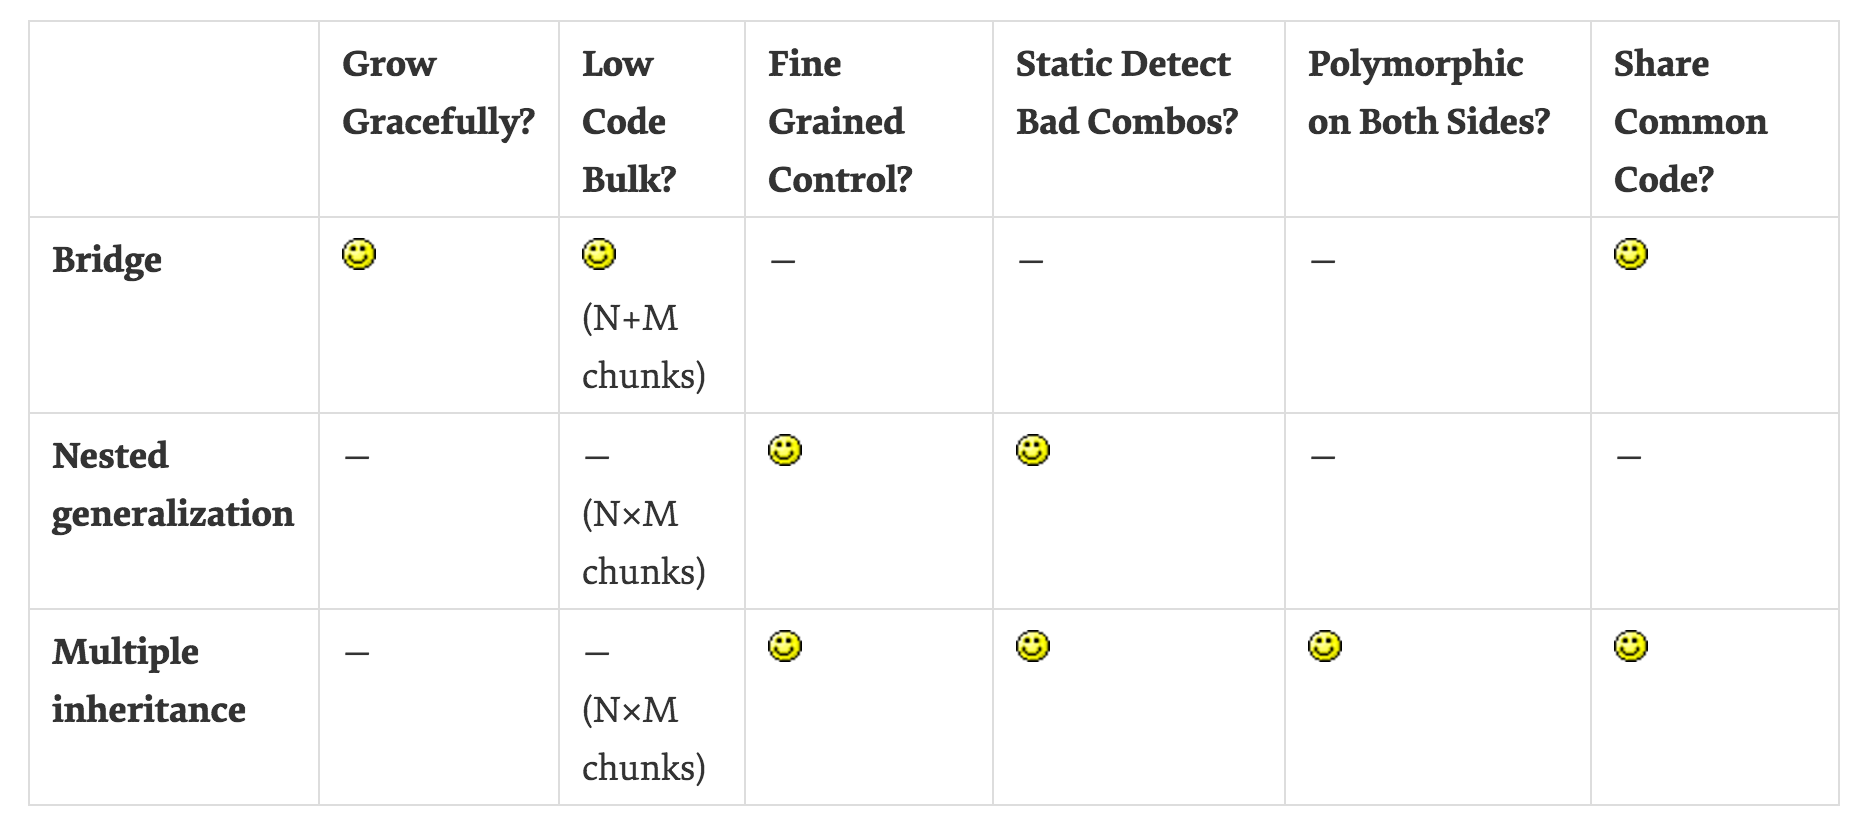
\includegraphics[scale=0.4]{pics/MI.png}

\item Try especially hard to use ABCs when you use MI. In particular, most classes above the join class (and often the join class itself) should be ABCs. In this context, "ABC" doesn’t simply mean "a class with at least one pure virtual function;" it actually means a pure ABC, meaning a class with as little data as possible (often none), and with most (often all) its methods being pure virtual.

\item Where in a hierarchy should I use virtual inheritance?  Just below the top of the diamond, not at the join-class.

\end{itemize}

\subsection{Interface}

\begin{itemize}

\item Nesting a class does not create a class member of another class. Instead, it defines a type that is known just locally to the class that contains the nested class declaration.  A good example is Class queue nest class node,  because node is just used inside the class Queue. Another good example is vector and it's iterator.

\item Virtual function must be member, operator\verb=>>= and \verb=<<= are never be members, or It maybe be a friend. Only non-member functions get type conversions on their left-most argument.  In the previous example, If you want to use support 2* obj, You need make operator * to be non member function.  Detail can be seen in effective c++.

 \item Keep in mind that only a class declaration can decide which functions are friends, so the class declaration still controls which functions access private data.

 \item Protect keyword don't use very often, it is just used in inheritance context. Child class can access base class protected member. you should use private keyword first if you real want to have good \textbf{Encapsulation} and \textbf{Never return reference or pointer to a private or protected member data.}

\item In C++ primer p653, you can see a good example class interface. You should remember it as a basic pattern.  If you use new allocate memory inside of your class, you should define: copy ctor, assignment operator and destructor, move copy ctor, and move assignment.

\begin{lstlisting}[frame=single, language=c++]
//below is string.h file
#pragma once
namespace Yan{
class String{
public:
String();  //default constructor
String(const char *a ); // specify constructor

String (const String &);  //copy ctor
String (String && other); //move copy ctor

String& operator=(const String &); //assignment
String& operator=(String&& other); //move assignment
String& operator=(const char*a); // option.

~String();  //usually, you should have these Seven member
               //functions if you use new inside your class.

friend ostream& operator<<(ostream & os, const String & st);
friend istream& operator>>(istream & is, String &st);

private:
const static int NUM= 1000; // const used inside of this class.
char* m_str;
	
};
ostream& operator<<(ostream & os, const String & st);
istream& operator>>(istream & is, String &st);
}
\end{lstlisting}

\begin{enumerate}
\item Put class definition into a namespace.
\item Use \#pragma once
\item You need to declare operator \verb=<<= inside of namespace outside of class
\item If you don't use smart pointer and allocate use new. you should follow five rules.( including move ctor and move assignment) if you class includes a resource.
\item Member function can access all the instance private data, such as other.m\_str, and no semicolon after each function.
\end{enumerate}


\begin{lstlisting}[frame=single, language=c++]
//user.cpp
String s;
s = "aaa"  //two actions
String s("aaa");   //one actions
String s{"aaa"};  // new feature in c++11
String s={"aaa"}; // same as previous one

String str; char temp[40];
str= temp // make it more efficient
\end{lstlisting}

\item String\& operator=(const char*a); is an option, why it make str=temp more efficient, see C++ Primer P652

\item  Friend has three categories:
\begin{enumerate}
\item Friend Class: just as TV and RemoteControl, you can declare RemoteControl a friend class inside TV.
\item Friend Member functions: You can select some member functions to be friend of another class, In this way, you need forward declaration.  When you write class TV;  It doesn't define a TV class, it just tell compile, TV is a class, definition can be done later.
\item Common Friend method, a good example is overload operator "<<"
\end{enumerate}

\item Prefer minimal classes to monolithic classes: big class is difficult to reach error-safe because it tackle multiple responsibilities. It's also difficult maintain, understand and deploy.
\begin{lstlisting}[frame=single, language=c++]
Class Matrix{
//100 member function.
} ; //bad design.

//Good design with small class with
nonmember function.
namespace MAT{
Class Matrix{
//core data and member function
}

Cal1(Matrix &);
Cal2(Matrix m1, Matrix m2)
......
}
\end{lstlisting}

\item Interface Principle: For a class X, all functions, including free functions, that both
1) "Mention" X 2) Are "supplied with" X  are logically part of X, because they form part of the interface of X.  In this definition, 1) Cal1 Mention X,  and 2) Cal1 in the namespace MAT, so caller can use ADL(argument depend lookup) loop Cal1 in namespace MAT, so \textbf{Cal1 is an interface of class Matrix, even it's not a member function of it.} Detail can be see in "exceptional C++ item31to item34.

\item Prefer writing nonmember nonfriend functions
\begin{enumerate}
\item operator =, ->, [], () must be members
\item needs a different type as its left-hand arguent, such as operator <<, use nonmember
\item leftmost argument needs type conversion, use nonmember
\item can be implement using the class public interface alone, use nonmember.
\end{enumerate}

\end{itemize}

\subsection{Special member functions}

\subsubsection{Basic}

\begin{itemize}

\item When you write a empty class, compiler will produce at least six member functions.  New compiler will produce move ctor and move assignment too.
\begin{lstlisting}[frame=single, language=c++]
class Empty{};

Empty();
Empty(const Empty& rhs);
Empty& oprator=(const empty & rhs);
Empty* operator&(){return this};
const Empty* operator&() const ;
~Empty();
\end{lstlisting}

\item Why you need to pay attention to these special member functions?  Given half a chance, the compiler will write them for you. Another reason is that C++ by default treats classes as value-like types, but not all types are value-like. Know when to write and disable them make you get correct code.

\item A good reference is "Everything You ever wanted to know about move semantics" in slideshare.net.

\item For these special member functions, main operations can be:
\begin{enumerate}
\item Compiler implicitly declare one
\item Use explicitly declare one
\item Once you define one, Compiler maybe Not declare another
\item You can ask compiler declare one
\item You can ask compiler delete one.
\end{enumerate}

\item First question is what "declare" mean?  \\
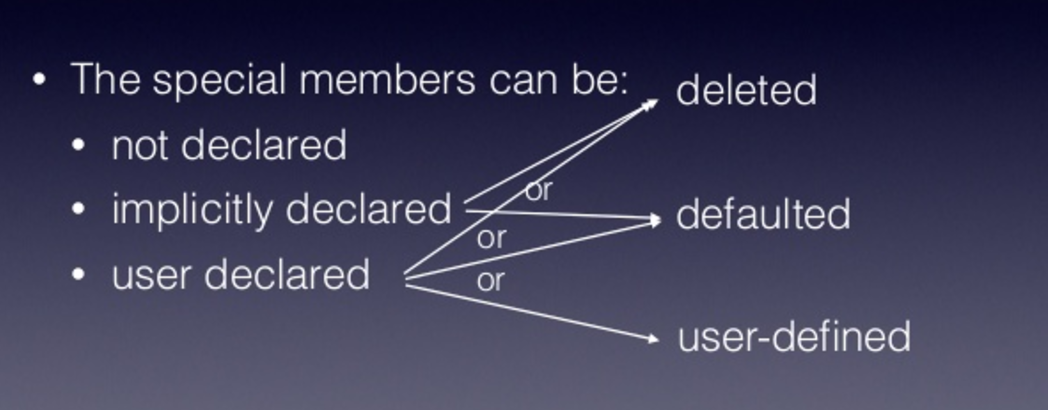
\includegraphics[scale=0.6]{pics/sm1.png} \newline

\item If you just define a class without any special member function, all six member function will be declared by compiler implicitly. \\
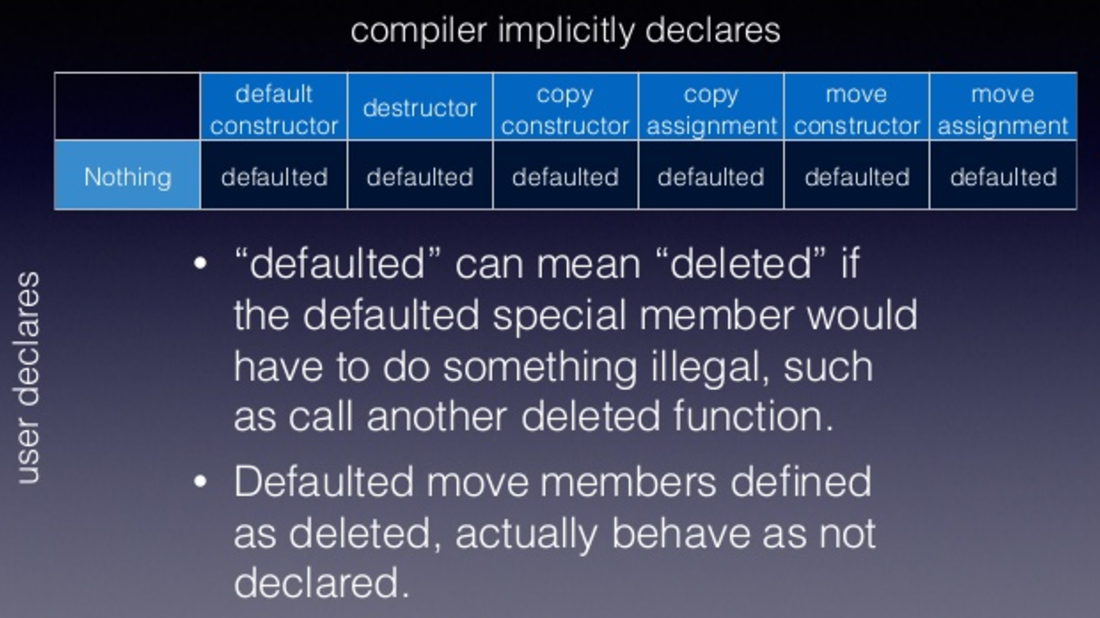
\includegraphics[scale=0.6]{pics/sm2.png} \newline

\item Why defaulted move member sometimes "deleted"? Detail can be found in "CWG 1402 is (imho) the most important bug fix to C++11". Another good article is google "Why is the move constructor neither declared nor deleted with clang? " In clang, it support C++11 standard better. 


\item Next question is what differences are between =default and user define empty ctor? problems of below code snippet are:
\begin{lstlisting}[frame=single, language=c++]
struct noncopyable  {
  noncopyable() {};
private:
  noncopyable(const noncopyable&);
  noncopyable& operator=(const noncopyable&);
};
\end{lstlisting}
\begin{enumerate}
\item The copy constructor has to be declared privately to hide it, but because it's declared at all, automatic generation of the default constructor is prevented. You have to explicitly define the default constructor if you want one, even if it does nothing.
\item Even if the explicitly-defined default constructor does nothing, it's considered non-trivial by the compiler. \textbf{It's less efficient than an automatically generated default constructor and prevents noncopyable from being a true POD type.}
\item Even though the copy constructor and copy-assignment operator are hidden from outside code, the member functions and friends of noncopyable can still see and call them. If they are declared but not defined, calling them causes a linker error.
\item Although this is a commonly accepted idiom, the intent is not clear unless you understand all of the rules for automatic generation of the special member functions.
\end{enumerate}


\item C++11 new keyword default and delete give below advantages:
\begin{lstlisting}[frame=single, language=c++]
struct noncopyable  {
  noncopyable() =default;
  noncopyable(const noncopyable&) =delete;
  noncopyable& operator=(const noncopyable&) =delete;
};
\end{lstlisting}
\begin{enumerate}
\item Generation of the default constructor is still prevented by declaring the copy constructor, but you can bring it back by explicitly defaulting it.
\item Explicitly defaulted special member functions are still considered trivial, so there is no performance penalty, and noncopyable is not prevented from being a true POD type.
\item The copy constructor and copy-assignment operator are public but deleted. It is a compile-time error to define or call a deleted function.
\item The intent is clear to anyone who understands =default and =delete. You don't have to understand the rules for automatic generation of special member functions.
\end{enumerate}


\item Another question is what differences are between =delete and "not declare" \\
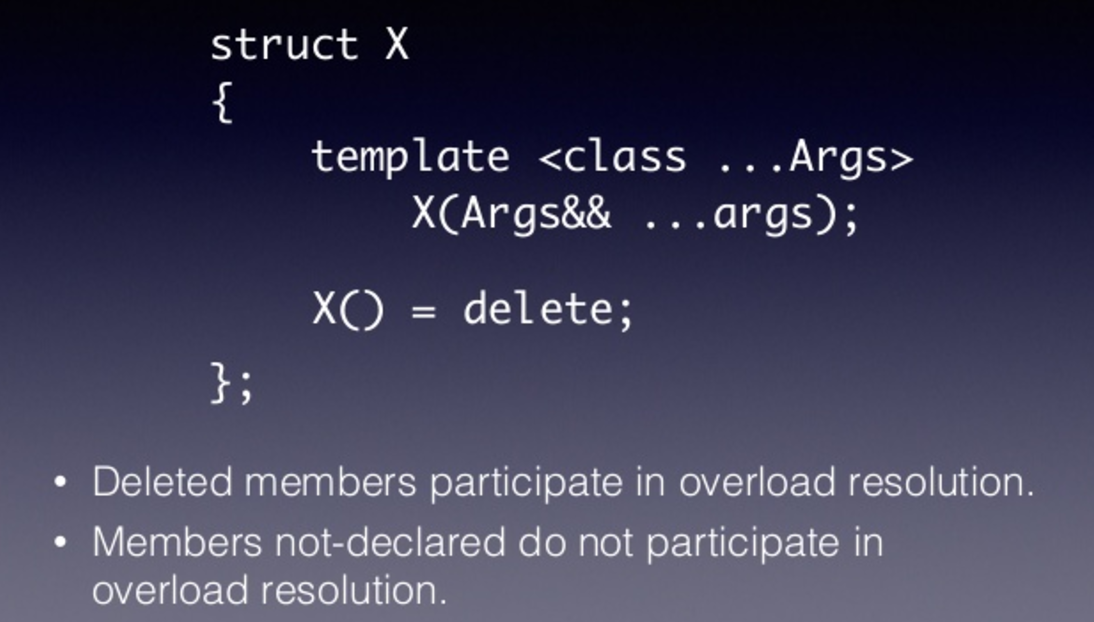
\includegraphics[scale=0.6]{pics/sm5.png} \newline

\end{itemize}
\subsubsection{Rules of implicitly declare }
\begin{itemize}
\item The Default ctor, will not be implicitly generated if:
\begin{enumerate}
\item you have explicitly declared any constructor.  Compiler doesn't create a default constructor if we write any constructor even if it is copy constructor.
\item There is a member in your class that is not default-constructible (such as a reference, a const object, or a class with no or inaccessible default constructor)
\item (C++11) you have explicitly told the compiler to not generate one using A() = delete;
\end{enumerate}


\item The copy ctor, will not be implicitly generated if:
\begin{enumerate}
\item you have explicitly declared a copy constructor (for class X a constructor taking X, X\& or const X\&)
\item there is a member in your class that is not copy-constructible (such as a class with no or inaccessible copy constructor)
\item (C++11) you have explicitly told the compiler to not generate one using A(const A\&) = delete;
\end{enumerate}


\item The Copy Assignment Operator will not be implicitly generated if
\begin{enumerate}
\item you have explicitly declared a copy-assignment operator (for class X an operator = taking X, X\& or const X\&) )
\item there is a member in your class that is not assignable (such as a reference, a const object or a class with no or inaccessible assignment operator)
\item (C++11) you have explicitly told the compiler to not generate one using A\& operator=(const A\&) = delete;
\end{enumerate}


\item The Destructor will not be implicitly generated if
\begin{enumerate}
\item you have explicitly declared a destructor
\item (C++11) you have explicitly told the compiler to not generate one using ~A() = delete;
\end{enumerate}

\item The Move Constructor or Move Operator(C++11) will not be implicitly generated if
\begin{enumerate}
\item you have explicitly declared a move constructor or move assignment(for class X, a constructor taking X\&\&)
\item there is a member in your class that cannot be moved (have deleted, inaccessible, or ambiguous)
\item you have defined a copy assignment operator, copy constructor, destructor, or move assignment operator
\item you have explicitly told the compiler to not generate one using A(A\&\&) = delete;
\end{enumerate}


\item The Move Assignment Operator (C++11) will not be implicitly generated if
\begin{enumerate}
\item you have explicitly declared a move assignment operator (for class X, an operator = taking X\&\&)
\item you have defined a copy assignment operator, copy constructor, destructor, or move constructor
\item you have explicitly told the compiler to not generate one using A\& operator=(A\&\&) = delete;
\end{enumerate}

\item  The justification is that declaring a copy operation (con‐struction or assignment) indicates that the normal approach to copying an object(memberwise copy) isn't appropriate for the class, and compilers figure that if memberwise copy isn't appropriate for the copy operations, memberwise move probably isn't appropriate for the move operations.

\item The same idea as the previous item, declaring a move operation (construction or assignment) in a class causes compilers to disable the copy operations.

\item The two copy operations are independent: declaring one doesn't prevent compilers
from generating the other. The two move operations are not independent. If you declare either, that prevents compilers from generating the other.

\item C++11 deprecates the automatic generation of copy operations for classes declaring
copy operations or a destructor. This means that if you have code that depends on
the generation of copy operations in classes declaring a destructor or one of the copy
operations, you should consider upgrading these classes to eliminate the dependence.
Provided the behavior of the compiler-generated functions is correct (i.e, if memberwise
copying of the class's non-static data members is what you want), your job is
easy, because C++11's "= default" lets you say that explicitly:

\item If you declared a destructor, implicitly defaulted copy member are deprecated.  \\
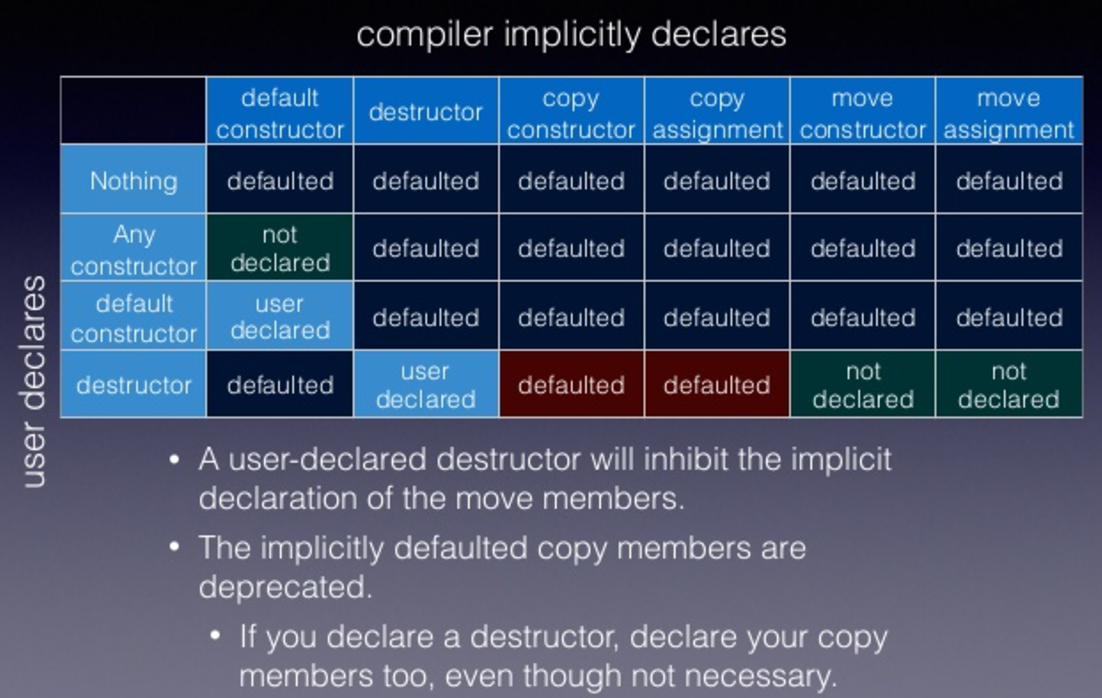
\includegraphics[scale=0.6]{pics/sm4.png} \newline


\item A summary can be seen blow \\
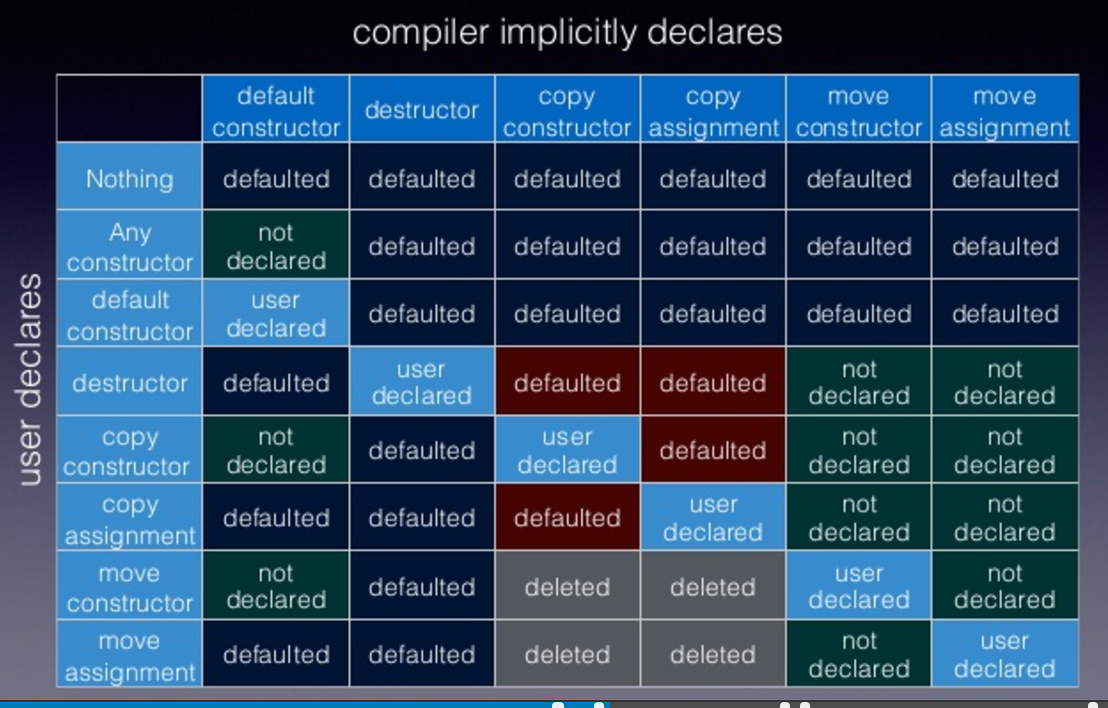
\includegraphics[scale=0.6]{pics/sm3.png} \newline

\end{itemize}

\subsubsection{initializer list}
\begin{itemize}
\item \textbf{Always use initializer list instead of assignment inside ctor.}

\item When to use member initalize list, you can see in this link:
\begin{enumerate}
\item to non-static const data members.
\item reference member
\item  member objects which do not have default constructor: (why I need default ctor can be explained here too)
\item need pass argument to base class ctor
\begin{lstlisting}[frame=single, language=c++]
class A {
    int i;
public:
    A(int );
};

// Class B is derived from A
class B: A {
public:
    B(int );
};

B::B(int x):A(x) { //Initializer list must be used
    cout << "B's Constructor called";
}
\end{lstlisting}

\item need to by copy between obj to member obj. (only one copy ctor, more efficient! see below source code.)
\end{enumerate}

\begin{verbatim}
http://www.geeksforgeeks.org/when-do-we-use-initializer-list-in-c/
\end{verbatim}

\begin{lstlisting}[frame=single, language=c++]
//method 1:
class(string &a, string &b): m_a(a),m_b(b){}
// just call string copy ctor,
//so you don't need string default ctor

//method 2:
class(string &a, string &b){   // two action.
m_a = a;  //call default constructor to build m_a
m_b = b; // then call assignment operator.
}
\end{lstlisting}

\item List member in a initialization list in the order in which they are declared in class. see effective c++ item 13. Order is important.

\item Member variables are always initialized in the order they are declared in the class definition. The order in which you write them in the ctor initialization list is ignored.  \textbf{So you'd better not have one member's initialization depend on other members}.
\begin{lstlisting}[frame=single, language=c++]
class Student{
string m_email;  //m_email will be init first, ingore order
string m_first_name;  // in the ctor initialization list.
Student(first_name) :m_first_name(first_name),
                m_email(m_first_anme+"@gmail"){}
\end{lstlisting}


\item If GetType() is a static member function, or a member function that does not use its this
pointer (that is, uses no member data) and does not rely on any side effects of construction (for
example, static usage counts), then this is merely poor style, but it will run correctly.

Otherwise (mainly, if GetType() is a normal nonstatic member function), we have a problem.
\textbf{Nonvirtual base classes are initialized in left-to-right order as they are declared}, so ArrayBase
is initialized before Container. Unfortunately, that means we're trying to use a member of the
not-yet-initialized Container base subobject.

\begin{lstlisting}[frame=single, language=c++, mathescape=true]
template<class T>
class Array : $\Hilight{23}$private ArrayBase, public Container

typedef Array AIType;
public:
Array( size_t startingSize = 10 )
: Container( startingSize ),
ArrayBase( Container::GetType() ),
\end{lstlisting}

\end{itemize}

\subsubsection{Basic routines}
\begin{itemize}
\item \textbf{Big five rule:} If you need customized copy ctor, assignment, and destructor, Then you also need move ctor and move assignment. Because it include memory allocation inside your class, you need you own copy ctor to perform deep copy and use move ctor to "move resource".

\item \textbf{Normally, ctor , destructor and assignment should be public. In inheritance context, all the base class desctructor should be virtual. }

\item Avoid calling virtual functions in ctor and dtor. "C++ Coding Standards" item 49.

\item What does a typical user defined move constructor do?
\begin{lstlisting}[frame=single, language=c++]
class x : public Base{
Member m_;
X(X&& x): Base(std::move(x)), m_(std::move(x.m_)){
x.set_to_resourceless_state();
}
}
\end{lstlisting}

\item What does a defaulted move assignment do?
\begin{lstlisting}[frame=single, language=c++]
class x : public Base{
Member m_;
X& operator=(X&& x) {
Base::operator=(static_cast<Base&&>(x));
m_ = static_cast<Member&&>(x.m_);
return *this;
}
}
\end{lstlisting}

%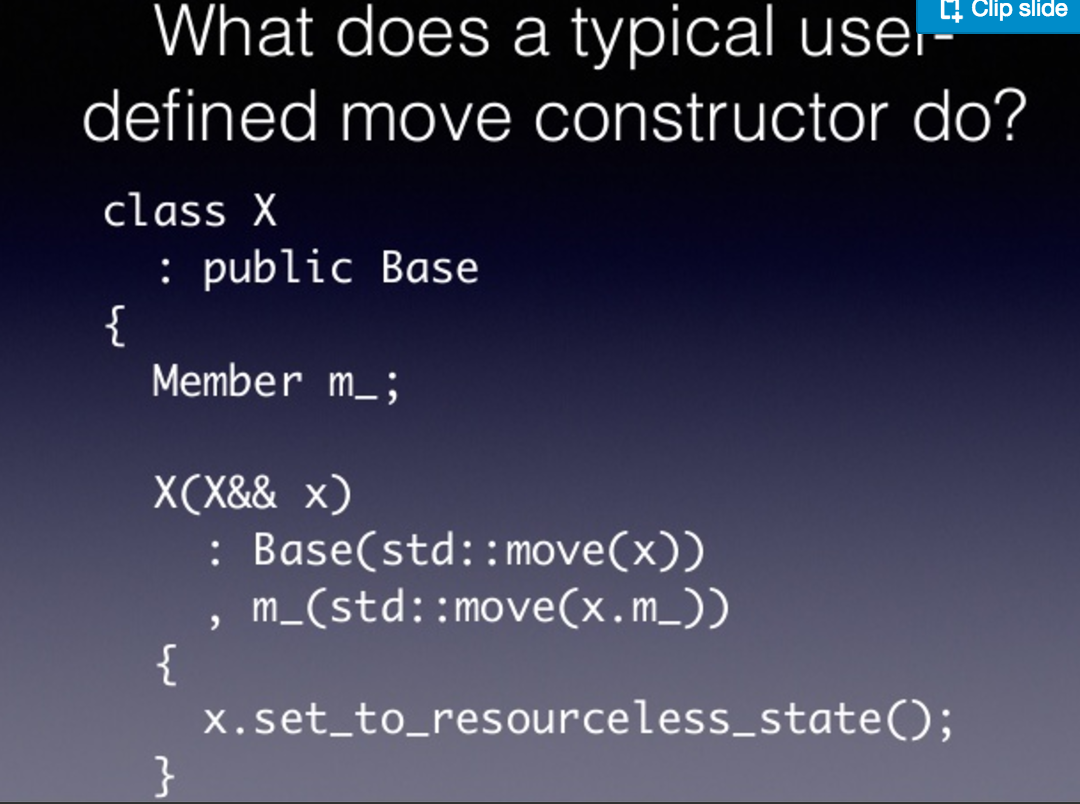
\includegraphics[scale=0.6]{pics/sm6} \newline
%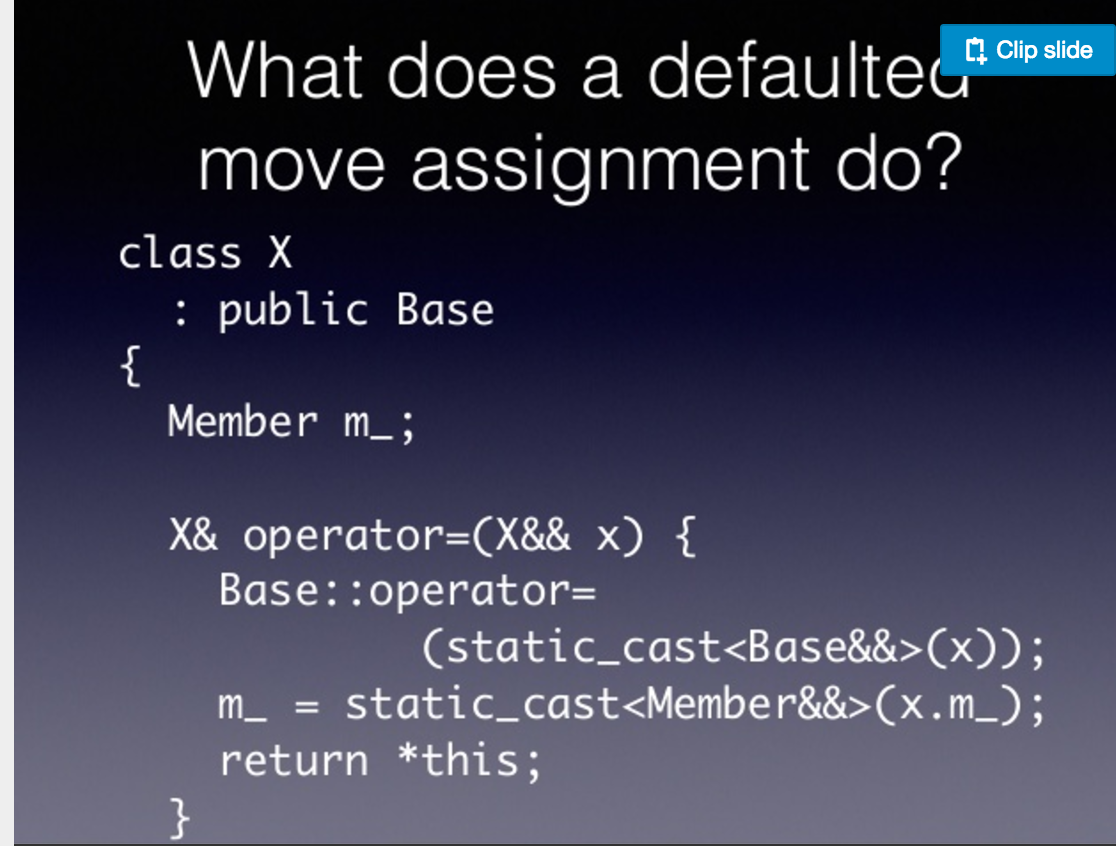
\includegraphics[scale=0.6]{pics/sm7} \newline


\item Assuming the only non-static data in the class is a std::string, here's the conventional way (i.e., using std::move) to implement the move constructor:
\begin{lstlisting}[frame=single, language=c++]
class Widget {
Widget(Widget&& rhs)
: s(std::move(rhs.s))
{ ++moveCtorCalls; }
private:
static std::size_t moveCtorCalls;
std::string s;
};
\end{lstlisting}

\item \textbf{If you define a specify ctor, you also need to define default ctor.} Because system will not produce any default ctor for you. So below statement will produce error when compiling.
\begin{lstlisting}[frame=single, language=c++]
class obj; //error
class* obj = new class(); //error
class arra[10] //error
template<class T>
class Array{
T t;
};

Array<class> a; //error
\end{lstlisting}

\item If no special demand, you can declare you own default ctor and use system implicit generated one. you can use keyword default
\begin{lstlisting}[frame=single, language=c++]
class Empty{
 Empty() = default;
 // you don't need to give implementation of default ctor.
 Empty(int i) ;
}
\end{lstlisting}


\item Make Constructors Protected to prohibit direct Instantiation. Make constructors Private to prohibit Derivation.

\item Use default arguments to reduce the number of ctor.
\begin{lstlisting}[frame=single, language=c++]
class Brush{
Brush();
Brush(Color c);
Brush(Texture t);

Brush(Color c= Black, Texture t = Solid); // it will be better.
}
\end{lstlisting}


\item From previous example, you can see that default ctor is very important. but when class MUST need another information when create, such as  worker class, You must provide SSN when you create a worker.
At this time, if you create default ctor, It's not good idea. A NULL SSN will cause a lot of trouble in the future.  So you have to use Worker pointer, and vector<Worker>.  You also need to use delete to disable default ctor.
That is C++ spirit, \textbf{You never have the best answer, only have context answer. }
\begin{lstlisting}[frame=single, language=c++]
class Worker{
char* SSN;
Worker(const char*);
Worker(){SSN=nullptr); //bad smell.
}
\end{lstlisting}

\item Normally you will have to explicitly declare your own destructor if:
\begin{enumerate}
\item You are declaring a class which is supposed to serve as a base for inheritance involving polymorphism, if you do you'll need a virtual destructor to make sure that the destructor of a Derived class is called upon destroying it through a pointer/reference to Base.
\item You need to release resourced aquired by the class during its leftime
Example 1: The class has a handle to a file, this needs to be closed when the object destructs; the destructor is the perfect location.
Exempel 2: The class owns an object with dynamic-storage duration, since the lifetime of the object can potentially live on long after the class instance has been destroyed you'll need to explicitly destroy it in the destructor.
\end{enumerate}


\item A copy constructor is called whenever a new variable is created from an object. This happens:

\begin{enumerate}
\item When a new object is initialized to an object of the same class.
\item When an object is passed to a functon by value.
\item When a function returns an object by value.
\item When the compiler generates a temporary object.
\end{enumerate}

\begin{lstlisting}[frame=single, language=c++]
1) Person r(p);   or  Person p = q;      // copy constructor
p = q;  // but not called in assignment; p has existed before

2) A value parameter is initialized from its argument.
fun(Person r)    fun(p);
// copy constructor, produce a new object r.
//just like Person r = p;

3) An object is returned by a function.
Person fun();
Person r = fun();
//here copy ctor is called twice.
// use -fno-elide-constructors in g++ produce two copy ctor
// or It will use Return value optimization.

4) class(string &a, string &b): m_a(a),m_b(b){}
//Initialization list
\end{lstlisting}

\item In previous example, you can see when you pass  value of obj, It will call copy ctor, It's not very efficient. So you should use reference or pointer if it's possible, don't pass object directly.


\item An Assignment operator examples: \textbf{1) avoid assignment self 2) return *this reference. }
\begin{lstlisting}[frame=single, language=c++]
class & class::operator=(class &a){
  if(this == &a)
    return *this;  //avoid assignment
    .............  // assignment operation here.
    return *this ; // return *this reference.
}
\end{lstlisting}

\item For reference, once assigned, a reference cannot be re-assigned. So if a class has a reference member, It can be initialized by initializer list in ctor and copy ctor. \textbf{But you can't overload assignment operator any more, If you really need assignment operator, change reference to pointer}

\end{itemize}


\subsection{special member functions in inheritance}

subsubsection{ctor}
\begin{itemize}

\item  \textbf{Subclass ctor will always call base class ctor.}

\begin{enumerate}
\item Constructor should NOT be virtual
\item If subclass doesn't define any ctor, compiler will implicitly define a default ctor, and this ctor will call base class default ctor.
\item If subclass has a ctor, but it doesn't explicitly call base specify ctor, ctor of subclass will call base default ctor.(without any parameter.) If base ctor only has specify ctor, no default ctor, produce compiler error.
\item If you want explicitly call base specify ctor, use initialization list syntax.

\end{enumerate}

\begin{lstlisting}[frame=single, language=c++]
class base{
public:
  base();  //default ctor
  base(int b); //specify ctor
private:
  int b;
};

class subclass: public base{
subclass();  //default ctor
subclass(int s, int b); // specify ctor1
subclass(int s);     //specify ctor2
int s;
};

subclass::subclass(int s, int b): base(b){
  m_s = s;
}
//////////////////////////////////////////
subclass sc1(2,3);
//call specify ctor1, then
// explicit call base specify ctor

subclass sc2(2);  // implicit call base default ctor
subclass sc3;   // implicit call base default ctor
// if base has not default ctor,
//sc2 and sc3 will produce error.
}
\end{lstlisting}
\item If you don't use  explicitly initialization list syntax to call base specify ctor, You will get uninitialized value or you can't initialize base member, Neither are good.
\begin{lstlisting}[frame=single, language=c++]
//method 2:
DeriveClass::DeriveClass(int base_a, b){
  //it will call base_class default constructor.
   // in this case, base_a is not assigned at all
   Derive_b = b
}	
/////////////////////
//method 3:
DeriveClass::DeriveClass(int base_a, b) {
base_a = a    //It can be thought as a bad design.
//You can't  access private base member data.
//base_a need to be public member data,
Derive_b = b
}
\end{lstlisting}

\item Idea behind rules: Do best to make sure a obj can be built.

\end{itemize}



\subsubsection{destructor}
\begin{itemize}
\item For destructor:
\begin{enumerate}
\item If a base class has a destuctor, but sub class doesn't have,  compiler will produce an implicit default destructor, and this implicit default destructor will call base class destuctor.
\item If you define a subclass destructor, It will call base destructor automaticlly, you don't need to call it explicitly.
\item The question is, How can you make sure you sub class destructor will be called if you use a base class pointer or reference, answer is below:
\end{enumerate}

\item Don't call base desctructor explicitly, It will called automatically in the reverse order of construction.  And you should give a base desctructor a definition, Or linker will report error it even you don't call it in your source code.

\item Make base class destructor public and virtual (polymorphic deletion by base class pointer or reference), or proteced and nonvirtual, base classes need not always allow polymorphic deletion. For example, consider class templates such as std::unary\_function. This time, you should make destructor protected and nonvirtual.
 \begin{lstlisting}[frame=single, language=c++]
template <class Arg, class Result>
struct unary_function{
  typedef Arg    argument_type;
  typedef Result result_type;
};

Illegal code that you can assume will never exist.
void f( std::unary_function* f ){
  delete f; // error, illegal
}
\end{lstlisting}

\item If base class still need to build itself, You can change it back public virtual,  Even without polymorphic deletion by now, you still need to declare it as virtual for the future safety(Even with a little dynamic-binding efficiency penalty. ) At same time, If a base class is not abstract class, usually, it's BAD design.

\item Never throw exception from dtor, if exception A is thrown, then stack-unwindling, when a obj is destructed, then dtor is called, when another exception B is thrown by the dtor, application will call terminat function immediately.  If you have exception, catch it inside of the dtor.

\end{itemize}

\subsubsection{copy ctor}

\begin{itemize}

\item copy ctor(assignment ctor) and slicing. Below four are all SLICING.  number 5 and number 4 is not very obvious. They are call base class ctor.  No matter what you input a reference to a derived class or not.
\begin{lstlisting}[frame=single, language=c++]
class Base{};
class Derived1 : Base{};
class Derived2 : Base{};
Derived1 d1;
Derived1 d2;
/////////////////////
Base b = d1; //1)

Fun(Base b);
Fun(d1);  //2)

Base& Bref = d1;
Fun(Bref) //3)

Base* bp = new B(Bref); //4)

Base* bp1 = new Derived1();  //5) sibling slicing
base* bp2 = new Derived2();
*bp1 = *bp2;  // bp1 just copy Base part in Derived2.
//so bp1 now is MIXTURE of d1 and d2.
\end{lstlisting}

\item Think a problem as below.
\begin{lstlisting}[frame=single, language=c++]
class Base{};
class Derived1 : Base{};
class Derived2 : Base{};
Derived d1;
Derived d2;

Base* Copy(Base& Bref){
//How to avoid slicing and make deep copy.
}

Base& Bref = d1
Base* d1p = Copy(Bref)

Base& Bref = d2
Base* d2p = Copy(Bref)
\end{lstlisting}

\item Continue- Think this problem: error method
\begin{lstlisting}[frame=single, language=c++]
Base* Copy(Base& Bref){
Base* p = new Base(Bref)
//Slicing happen. bad
}
\end{lstlisting}
\item Continue- Think this problem: TypeID method.
\begin{lstlisting}[frame=single, language=c++]
Base* Copy(Base& Bref){
//Use tyid and dynamic_cast
//involve a lot of if and switch about type.
//anytime if you use dynamic_cast and if,
//you can think about virtual function
}
\end{lstlisting}

\item Continue- Think this problem: Virtual Clone method.
A function's return type is never considered part of its signature. You can override a member
function with any return type as long as the return type could be used wherever the base class
return type could be used.
\begin{lstlisting}[frame=single, language=c++, mathescape=true]
class Base{
  virutal Base* Clone() = 0;
};

class Derived1 : Base{
    virutal $\Hilight{4}$Derived1* Clone(){return new Derived1(*this);}
}

Base* Copy(Base& Bref){
Base* p = Bref.Clone();
}
\end{lstlisting}


\item Continue- Think this problem: Change Design. Base is concrete class,  More Effective C++ Item 33 said"Making Non-leaf class abstract. So maybe you can change the inheritance system.

\item copy ctor and copy initilization. Detail can be found "Is there a difference in C++ between copy initialization and direct initialization?"
\begin{lstlisting}[frame=single, language=c++]
class A{
explicit A(const &A);
}
A a1;
A a2(a1) //OK
A a3 = a1 //doesn't work
\end{lstlisting}
\item Assignment operator and copy ctor in inheritance:
\begin{enumerate}
\item \textbf{Default Assignment  operator and  copy constructor in derived class which are implicitly produced by compiler will call default base assignment  operator and  copy constructor.}

\item \textbf{If derived class has no new operation. Don't need to define derived class Assignment  operator and  copy constructor, implicit one will call base one automatically}

\item \textbf{If derived class has new operation. You have to define derived class Assignment  operator and  copy constructor, it will not invoke assignment  operator and  copy constructor in base class any more.  Inside, manually invoke base class Assignment operator and copy ctor } Detail can be found in C++ primer p760. Syntax looks like below: see effective C++ Item 16.

\item For copy ctor, just init list syntaxt. For assignment operator, use two different methods depends on if base class declare its own assignment operator(). Source code is below:

\begin{lstlisting}[frame=single, language=c++]
DerivedClass::DerivedClass(const DerivedClass &dc): \
BaseClass(dc){...}  //init list syntax here.

DerivedClass & DerivedClass::operator=(const DerivedClass &dc){
BaseClass::operator=(dc);
// base class declare explicitly operator

( (BaseClass&) *this ) = dc
//base class no explicitly operator
// change *this to BaseClass reference,
// if you change to BaseClass, It will call copy ctor.
}
\end{lstlisting}

\end{enumerate}
\end{itemize}

\subsection{RAII}
\begin{itemize}
\item Whenever you deal with a resource that needs paired acquire/release function call, encapsulate that resource in an object.  Such as: fopen/fclose, lock/unlock, and new/delete.

\item When implementing RAII, be conscious of copy construction and assignment. the compiler-generated version probably won't be correct. If it's not copyable, use =delete , if it's copyable, duplicate the resource.  You also can use smart\_pointer in this scenario too.

\item The basic idea of RAII  is to represent a resource by a local object, so that the local object’s destructor will release the resource.  That is to say: To prevent resource leaks, use RAII objects that acquire resources in their constructors and release them in their destructors.
\begin{lstlisting}[frame=single, language=c++]
//C version,
File* fp = fopen("/path/to/file");
// throw exception here, then resource leaking
fclose(fp);

//Java version
try {
    File file = new File("/path/to/file");
    // throw exception here, go to finally.
} finally {
    file.close();
}

//c++ version
fun{
fstream if("path/to/file")
if.getline
// you don't need to if.close().
}

//c++ smart version.
std::unique_ptr<FILE,          // <-- the wrapped raw pointer type: FILE*
                int(*)(FILE*)> // <-- the custom deleter type: fclose() prototype
myFile( fopen("myfile", "rb"), // <-- resource (FILE*) is returned by fopen()
        fclose );              // <-- the deleter function: fclose()
\end{lstlisting}

\item Another good example RAII is unique\_ptr. The idea of smart pointer is putting *p into a local pointer-like object, then when it go out scope or unwind-stack when exception is thrown, It will call destructor, then delete p.

\item We should consider resource generically, pointer *p pointed to a new object is resource, A handle to a file is a resource to. \textbf{We wrap handle to a file into ifstream, and wrap pointer *p into smart\_pointer}

\item Just like return value,  Exception will skip all the statement below the throw, In C++, It doesn't support finally statement sometimes. At this time, we need to use RAII.
\begin{lstlisting}[frame=single, language=c++]
Int *p = new int;
string a   //a is ok, a will be destructed properly
              //due to the C++ unwind stack.
throw exception.
delete p; // this will not run.
\end{lstlisting}

\item For this problem, you should use smart pointer to declare a auto object.  If you use string object, It's ok.  So in previous example,  you can use smart pointer, it will help you to avoid memory leakage problem.
\begin{lstlisting}[frame=single, language=c++]
unique_ptr<int> aupr (new int(100);
string a   //a is ok, a will be destructed properly
              //due to the C++ unwind stack.
throw exception.
// both a and aupr will call their own destructor  function.
\end{lstlisting}

\item In you ctor, If you use new and new failed and throw a exception, the destructor will not be called. You can use auto\_ptr as member data and use init list to initialzie it. see  more effective C++ exception chapter.

\item Don't use C FILE* and char [] as string. Use iofile class and string object, because they are exception safe
\begin{enumerate}
\item Any time when you use new, consider if there are c++ container or object.
\item If not, use smart\_pointer.
\end{enumerate}

\item Another example is when you make program based on Win API.
\begin{lstlisting}[frame=single, language=c++]
class module {
public:
    explicit module(std::wstring const& name)
    : handle { ::LoadLibrary(name.c_str()) } {}

    ~module{
       ::FreeLibrary();
    }
private:
    HMODULE handle;
};
\end{lstlisting}

\item There are three RAII implementation instances in your practical programming:
\begin{enumerate}
\item Use auto member; You have to keep m\_str and vc are RAII.  In this way, you don't need to build dtor manually.
\begin{lstlisting}[frame=single, language=c++]
class RAII {
private:
    string m_str;
    vector<int> vc;
};
\end{lstlisting}

\item Use pointer and handle; In this way, You have to use pointer, Maybe you need some customized action in runtime , \textbf{Use handle is only method to use this resource} or any other reason. And this time, you have to write your own dtor.
\begin{lstlisting}[frame=single, language=c++]
class RAII {
private:
    string* m_str;
    vector<int*> vc;
};
\end{lstlisting}

\item Use smart point wrap pointer and handle; When you wrap handle, you can custom this delete behavior. See source code below:
\begin{lstlisting}[frame=single, language=c++]
class RAII {
private:
    unique_ptr<string>  m_str;
    vector<unique_ptr<int> > vc;
};
\end{lstlisting}

\begin{lstlisting}[frame=single, language=c++]
class module {
public:
    explicit module(std::wstring const& name)
    : handle { ::LoadLibrary(name.c_str()) } {}
private:
using module_handle = std::unique_ptr<void, decltype(&::FreeLibrary)>;
   module_handle handle;
};
\end{lstlisting}
\end{enumerate}

\item Another question is ownership of resource:
\begin{enumerate}
\item For auto member resource: \textbf{1)Same life duration(RAII), 2)exclusive ownship to a single obj, but it's copyable(A a1 = a2).  3)move with efficiency(A a1 = A() ) }. If auto member has it's own copy and move special function, You don't need to write any special function in your class. You follow the "Rule of Zero".

\item For raw pointer and handle: \textbf{1) default copy ctor will cause two pointer or handle refer the same resource, It's absolutely BAD SMELL of code 2) So you have to follow "Rule of five" to build your special member function. 3) After you build five special member function, you get RAII and exclusive ownship to a single object, and copyable and efficient move}
\begin{lstlisting}[frame=single, language=c++]
Class RawPointer{
...........
RawPointer(const RawPointer& rhs){
pRes = new Resource( *(rhs.pRes));
}

RawPointer(RawPointer&& rhs){
pPes = rhs.pRes;
rhs.pRes = nullptr;
}
private:
Resource* pRes;
}
\end{lstlisting}

\item For uniqu\_ptr; \textbf{1) Same life(RAII) 2)exclusive ownship but not copyable 3) uniqu\_ptr support move operation. } You still follow "rule of zero"

\item Even with uniqu\_ptr member, If you follow "rule of zero", that is to say that you don't provide any customized special member function, then the class is not copyable. But if you build copy ctor by youself, get raw pointer from origin side, and build a new uniqu\_ptr member from origin side's raw pointer, you can implement copyable, and code smell better than raw pointer with "Rule of Five". So in this way, \textbf{It's not recommended to use raw pointer in RAII and ownership context}.

\item For shared\_ptr; \textbf{1) Not a RAII 2) shared ownship, 3) copyable and moveable}. When you move a shared\_ptr, origin one is set to nullptr and ref count doesn't increas.  You still follow "rule of zero".

\end{enumerate}

\item \textbf{ Conclusion, If you consider RAII and ownship at the same time, thing will become complex}  so I would like to give you some examples to illustrate them.

\begin{enumerate}
\item Prefer to use auto member for most of time! It follow "Rule of Five" and support copyable and movable.

\item  For special demand, for example Car class,  people can \textbf{custom} its engine, and buy \textbf{two} at the same time. In this context, you car class should use raw pointer, 1) auto member doesn't support custom 2) uniqu\_ptr doesn't support copyable.  And you have to follow "Rule of Five"
\begin{lstlisting}[frame=single, language=c++]
class Car{
//follow "Rule of Five"
Engine *pEn;
~Car(){delete pEn} // assure RAII
}
\end{lstlisting}

\item For special context, It doesn't support object copy: for example 1) Person class in semantic;  2) other  perform consideration, Class Big{int [30000];};  3) Other implementation constrain, such as iostream class.   Under such context, you can use uniqu\_ptr to manage the resource and implement uncopyable.
\begin{lstlisting}[frame=single, language=c++]
class Person{
uniqu_ptr<Resource> pRes;
}
\end{lstlisting}

\item For special context, shared resource, you can use shared\_ptr.  You still can follow "Rule of zero" and resource will be deleted when ref count is 0.
\begin{lstlisting}[frame=single, language=c++]
class Student{
shared_ptr<SchoolBus> pBus
}
\end{lstlisting}

\item To know semantic of two smart pointers. Don't use them just replace raw pointer.
\end{enumerate}

\end{itemize}

\section{Generic programming}
\subsection{Template basic}
\begin{itemize}
\item For C++, one plus is polymorphism, the other is generic code. and generic programming is mainly based on template. 

\item A simple way to simulate template is \verb=typedef int Item=; But when you change the data type, you need to change header file, and you can't have int and double to template class at the same programme. so C++ introduces a better method: template<typename T>.

\item You should use templates if you need functions or container class(act likes) that apply the same algorithm to a variety of types. Templates are frequently used for container classes because the idea of type parameters matches well with the need to apply a common storage plan to a variety of types.

\item Use typename, not class. At the same time. simple names, such as T.
\begin{lstlisting}[frame=single, language=c++]
template<typename T> swap(T& a, T&b){
.........
}
\end{lstlisting}

\item You can have several kinds of template parameters.
\begin{enumerate}
\item  Type Parameters.
  	\begin{enumerate}
   	\item Types
    \item  Templates (only classes and alias templates, no functions or variable templates)
	\end{enumerate}

\item Non-type Parameters
   \begin{enumerate}
	\item Pointers
	\item References
	\item Integral constant expressions
	\end{enumerate}
\end{enumerate}

\item You can use more than one type parameter, or Default Type Template Parameters
\begin{lstlisting}[frame=single, language=c++]
template <typename T1,  typename T2>
class Pair{ }
Pair<double, int> pair1;

template <typename T1,  typename T2=int>
class Pair{ }
Pair<double> pair2;
\end{lstlisting}

\item you can use Non-Type Argument in a template. But it will cause code bloat problem. 
\begin{lstlisting}[frame=single, language=c++]
template <typename T, int n>
class ArrayTP{
T ar[n];
......
}
\end{lstlisting}

\item type parameter can be another template calss.  It's different with "template template parameter" which is introduced below.
\begin{lstlisting}[frame=single, language=c++]
template<typename T> // int T is here
class A

template<typename T> //A<int> is T here.
class B

B< A<int> > obj;
//Two T has no any relationship.
//you can give them any better description name
//just like vector< vector<int> >. 
\end{lstlisting}

\item Another usage is template template parameter. An article is "Correct usage of C++ template template parameters".

\item template class can be used as base class and used as a component class.
\begin{lstlisting}[frame=single, language=c++]
template< typename Type>
class SpecialStack: public Stack<Type>{
Array<Type> array;
}
\end{lstlisting}

\end{itemize}

\subsubsection{template instantiation}
\begin{itemize}
\item \textbf{compiler will parse the template definition before it instantiation.} Why? It's a compiler, not a macro processor. One problem with that is that errors in the template itself won't be detected as long as it is only instantiated with 'friendly' types that don't trigger the errors: for example, if the template assumes that the type always has such-and-such a method.

\item That is very important for you to understand three examples in the article "Dependent name lookup for C++ templates". When compiler see T::foo\_method, \textbf{he will not just specify T as Foo.} Think that your are compiler, you just delete the whole struct Foo, then try to understand it. 
\begin{lstlisting}[frame=single, language=c++]
struct Foo {
    template<typename U>
    static void foo_method(){
    }
};

template<typename T> void func(T* p) {
    // A. error: expected primary-expression before ‘>’ token
    // T::foo_method<T>();

    // B. works!
    T::template foo_method<T>();
}
\end{lstlisting}

\item template can't be compiled. only when you declare a variable, It will instantiation. (It will make compiling time longer). So all the template definition must be put in head file.

\item C++ use implicit or explicit instantiation to generate a specialized class or function definition from template
For implicit, you have to declare an obj, but for explicit, you don't need to declare an obj; \textbf{declare an object or use template}. 

\begin{lstlisting}[frame=single, language=c++]
ArrayTP<int, 100> stuff //implicit instantiation
// you have to declare obj stuff.

template ArrayTP<string, 100>;
//generate a specialized class even you don't declare an obj
\end{lstlisting}


\item C++ Coding standards 65 states customization of point. In order to understand it. You need to understand two some basic conception: "two phases lookup" and "dependent name".  

\item two phases lookup can see "Dependent name lookup for C++ templates" in the ref and "Two-Phase or Not Two-Phase:
The Story of Dependent Names in Templates" in the ref.
\end{itemize}

\subsubsection{template specialization}
\begin{itemize}
\item Class templates can be partially specialized, and the resulting class is still a template. Partial specialization allows template code to be partially customized for specific types in situations, such as:

\begin{enumerate}
\item A template has multiple types and only some of them need to be specialized. The result is a template parameterized on the remaining types.

\item A template has only one type, but a specialization is needed for pointer, reference, pointer to member, or function pointer types. The specialization itself is still a template on the type pointed to or referenced.
\end{enumerate}

\item Difference between template function overload and partial specializations
\begin{enumerate}
\item partial specializations is just use in template class.
\item partial specializations need put another <> after class name
\item If you want to have custom implementation of function with same name, use overload function, if you need  custom implementation of class with same name, use partial specialization.
\begin{lstlisting}[frame=single, language=c++]
template <typename T1, typename T2>
class Pair{}  //general one

tempalte <typename T1>
class Pair<T1, T1>  // partial specializations

tempalte <typename T1>
class Pair<T1, int > // partial specializations
//-------------------------------------------

tempalte <typename T>
class Foo //general one

tempalte <typename T*>
class Foo //partial specializations.
\end{lstlisting}

\end{enumerate}

\item Explicit specialization include complete specialization and partial specialization.
\begin{lstlisting}[frame=single, language=c++]
template<> class Pair<int,int>{...}; //complete specialization
template<typename T1> class Pair<T1, int>{...}; //Partial
\end{lstlisting}

\item Non type argument and default type argument only define one template body(only one recipe). But Specialization need to define a generic template body(one recipe), For another type, It need to define a different template body(another recipe), because the code will be different with generic one.

\textbf{Instantiation is different with specialization.  For instantiation, it will use template function to produce function body, but for specializaiton, you have to redefine you own function body }

\begin{lstlisting}[frame=single, language=c++]
Template<typename T>
      void sortedArrary (T) {...};

template void sortedArray<Person>(Person) // instantiation
template<> void sortedArray<Person>(Person){ // specialization.
.... //give you own definition of fun body.
};
\end{lstlisting}

\item keep the design of a template in mind and not use it blindly. When you input pointer as typename, you should be on high alert.


\item Explicit specification usually need define all the implementation in it. If there is a lot of repetition. There are two another options: 
\begin{enumerate}
\item Add a special function just suitable for certain type. 
\begin{lstlisting}[frame=single, language=c++]
template <typename T>
class A{
public:
    void onlyForInts(T t){
        static_assert(std::is_same<T, int>::value, "Works only with ints!");
    }

protected:
    std::vector<T> myVector;
};

int main(){
    A<int> i;
    i.onlyForInts(1); // works !

    A<float> f;
    //f.onlyForInts(3.14f); // does not compile !
}
\end{lstlisting}

\item Use type trait and overload, select at the compile time. See enable\_if example below.

\end{enumerate}



\item decltype and  Trailing Return type(C++11 new feature)
\begin{lstlisting}[frame=single, language=c++]
template<typename T1, typename T2>
void f(T1 x, T2 y){
decltype(x+y) xpy = x+y;
}

//with return value;
template<typename T1, typename T2>
auto f(T1 x, T2 y) ->decltype(x+y)
{
  x+y;
}
\end{lstlisting}

\item How to make your template class has more generic use for client, "exceptional C++" item 5 introduces more idea in this topics.

\end{itemize}



\subsection{Template function}
\begin{itemize}
\item When you use template function with real argument, compiler will extract type information from real argument, then generate real function code for you.  So it will make compiler looks longer.
\begin{lstlisting}[frame=single, language=c++]
swap(i1, i2);
swap(f1, f2);
// don't need to specify int, compiler
//can extract type information from i1

// compiler will produce two swap functions bodies.
\end{lstlisting}

\item Why we need a overload template function, Because not all type support the same operator. For example, in your template function, you use = operator, but when you use array for this template function type, compiler will report error.
\begin{lstlisting}[frame=single, language=c++]
template <typename T>
void swap(T a[], T b[], int n)

template <typename T>
void swap(T &a, T &b )
\end{lstlisting}

\item Overload is different with Specializations, Overload means that you have different function signatures. Specialization have the same function signature.

\item "Why Not Specialize Function Templates?" You can see it in the ref.

\item "Why Argument Dependent Lookup doesn't work with function template dynamic\_pointer\_cast". See it in the ref

\item "C++ template function taking template class as parameter" See in ref.
\end{itemize}


\subsubsection{overload resolution}
\begin{itemize}
\item Given a function name, you can have regular, template and explicit specialization temple. When pick a function, regular> specialization> template. function picking ranking from best to worst is:
\begin{enumerate}
\item Exact math, regular function
\item Template if you have define the same template function name.
\item Conversion by promotion
\item Conversion by standard conversion.
\item user-defined conversion.s
\end{enumerate}

\item What is exact match. There are table below:

\begin{tabular}{|c|c|}
\hline
Actual argument & Formal argument \\
\hline
type-name & type-name \& \\
\hline
type-name \& & type-name \\ \hline
type-name [ ] &  type-name* \\ \hline
type-name ( argument-list ) & ( *type-name ) ( argument-list ) \\ \hline
type-name  & const type-name \\ \hline
type-name  &  volatile  type-name \\ \hline
type-name*  & const type-name*  \\ \hline
type-name*  & volatile  type-name*  \\  \hline
\end{tabular}

\item About exact match, there are three result:
\begin{enumerate}
\item If there are two exact matches, compiler can't distinguish them, then it will report error
\item If reference and pointer, even there are two exact match, It will pick up first according to const.
\begin{lstlisting}[frame=single, language=c++]
int i = 2;

f(const int& j); //#1
f(int& j);  //#2, 2 will be selected, because i isn't const
\end{lstlisting}
\item If there are exact match, it will pick up before template, even template has EXACT specification.
\end{enumerate}

\item For temple, order is:
\begin{enumerate}
\item specialized argument template
\item specialization version in side this  specialized argument template.
\end{enumerate}
\begin{lstlisting}[frame=single, language=c++]
template<typename T>
f(T t);  //#1
template< >f<int*>(int* t) #2

template<typename T>
f(T* t); //#3

template<> f<int> f( int* t) //#4

int * p;
f(p) // #4>#3>#2>#1
\end{lstlisting}

\item For above example, If you omit type inside <> after function name f, It will depends on location.
\begin{lstlisting}[frame=single, language=c++]
template<typename T>
f(T t);  //#1

template< >f<>(int* t) //#2 is specialization of #1
/////////////////////////////////////////
template<typename T>
f(T* t); //#3

template< >f<>(int* t) //put here is specialization of #3
\end{lstlisting}

\item You can tell compiler that you prefer template function over overload one

\begin{lstlisting}[frame=single, language=c++]
template<typename T>
void f(T t);  //#1

void f(int t) //#2

f<>(2) //tell compiler use #1, not #2.
\end{lstlisting}

\end{itemize}


\subsubsection{template function specification}
\begin{itemize}

\item Explicit Specialization: Because for char *, you can't use > , but use strcmp.  So you need to build explicit Specialization Version. The prototype and definition of an explicit spcialization should be preceded by template<> and should mention the specialized type by name.
\begin{lstlisting}[frame=single, language=c++]
Template<typename T>
      void sortedArrary(T) {...};

template<> void sortedArray<const char *>(){...}
\end{lstlisting}

\item Some explicit specification syntax.
\begin{lstlisting}[frame=single, language=c++]
template<typename T>
void foo(T param);

//syntax 1: not a specialization, it is an overload
void foo(int param);

//syntax 2: ill-formed, not recommend
void foo<int>(int param);

//syntax 3: normal explicit specialization, specify T directly
template <> void foo<int>(int param);

//syntax4: same as above, but use template argument deduction
template <> void foo(int param);

//syntax5: same as above, but use template argument deduction
template void foo(int param);
\end{lstlisting}

\item There seems to be (a lot) of confusion regarding explicit instantiation and specialization. The code I posted above deals with explicit instantiation. The syntax for specialization is different. Here is syntax for specialization: Note that angle brackets after template!

\begin{lstlisting}[frame=single, language=c++]
template <typename T> void func(T param) {} // definition

template void func<int>(int param); // explicit instantiation.

template <> void func<int>(int param) {} // specialization
\end{lstlisting}

\item  If you want to customize a function base template and want that customization to participate in overload resolution (or, to always be used in the case of exact match), make it a plain old function, not a specialization. And, if you do provide overloads, avoid also providing specializations. Detail you can google" Why Not Specialize Function Templates?" \textbf{prefer to use overload than template function specification.}

\item template function only support full specification. 
\end{itemize}

\subsubsection{summary}
\begin{itemize}
\item First name look up, then overload, last instanitiation.

\item A good article is "Overload resolution" in Andrzej's C++ blog. \textbf{It taught you 1) name kookup and 2)overload and 3)instanition
three conception very well.}

\item You can see a visio fig in the pics directory. 

\item p1 and p2, 
\begin{lstlisting}[frame=single, language=c++]
template <typename T> struct Base {
   typedef int MyType;
};

template <typename T> struct Derived : Base<T> {
   void g() {
       // A. error: ‘MyType’ was not declared in this scope
       // MyType k = 2;

       // B. error: need ‘typename’ before ‘Base<T>::MyType’ because
       // ‘Base<T>’ is a dependent scope
       // Base<T>::MyType k = 2;

       // C. works!
       typename Base<T>::MyType k = 2;

       std::cerr << "Derived<T>::g --> " << k << "\n";
   }
};
\end{lstlisting}

\begin{lstlisting}[frame=single, language=c++]
struct Foo {
    template<typename U>
    static void foo_method()
    {
    }
};

template<typename T> void func(T* p) {
    // A. error: expected primary-expression before ‘>’ token
    // T::foo_method<T>();

    // B. works!
    T::template foo_method<T>();
}
\end{lstlisting}



\item p3
\begin{lstlisting}[frame=single, language=c++]
template <typename T> struct Base {
   void f() {
       std::cerr << "Base<T>::f\n";
   }
};

template <typename T> struct Derived : Base<T> {
   void g() {
       std::cerr << "Derived<T>::g\n  ";
       f(); //error happen here. 
       this->f() will resolve problem.
   }
};
\end{lstlisting}


\item p4 name look up has two stages. 1) from process function, then it found a) current namespace, b)using namespace and c)all previous declaration.  At these time only f(T) is visible, Then add it into overload options.  2) When T is knowing, It will search all options in the boost namespace, \textbf{At this time, it will not search framework namespace again}
\begin{lstlisting}[frame=single, language=c++]
namespace framework  // library 1{
  template <typename T>
  void f(T) { puts("master"); }
 
  template <typename T>
  void process(T v) { f(v); } 
}
 
namespace boost      // library 2{
  template <typename T>
  struct optional {};
}
 
namespace framework  {     
  template <typename T>
  void f(boost::optional<T>) { puts("optional<T>"); }
    
  inline
  void f(boost::optional<bool>) { puts("optional<bool>"); }
}
 
int main()           // our program logic{
  int i = 0;
  boost::optional<int>  oi;
  boost::optional<bool> ob;
  
  framework::process(i); //output three master
  framework::process(oi);
  framework::process(ob);
}
\end{lstlisting}


\item p5, In instaniation, with help of ADL, boost namespace is searched and two other functions are added into overload options.

\begin{lstlisting}[frame=single, language=c++]
namespace framework  // library 1
{
  template <typename T>
  void f(T) { puts("master"); }
 
  template <typename T>
  void process(T v) { f(v); } 
}
 
namespace boost      // library 2
{
  template <typename T>
  struct optional {};
}
 
namespace boost      // some glue between 1 and 2
{     
  template <typename T>
  void f(optional<T>) { puts("optional<T>"); }
    
  inline
  void f(optional<bool>) { puts("optional<bool>"); }
}
 
int main()           // our program logic
{
  int i = 0;
  boost::optional<int>  oi;
  boost::optional<bool> ob;
  
  framework::process(i);
  framework::process(oi);
  framework::process(ob);
}
\end{lstlisting}

\item p6 template specfication happen in the end and after overload. 
\begin{lstlisting}[frame=single, language=c++]
namespace framework  // library 1
{
  template <typename T>
  void f(T) { puts("master"); }
 
  template <typename T>
  void process(T v) { f(v); } 
}
 
namespace boost      // library 2
{
  template <typename T>
  struct optional {};
}
 
namespace framework  // some glue between 1 and 2
{     
  template <>
  void f<boost::optional<bool>>(boost::optional<bool>)
  { puts("optional<bool>"); }
}
 
int main()           // our program logic
{
  int i = 0;
  boost::optional<bool> ob;
  
  framework::process(i);
  framework::process(ob);
}
\end{lstlisting}

\end{itemize}



\subsection{template and inheritance}



\subsubsection{Templates Parameterised by base class}
\begin{enumerate}
\item private heritance 
\begin{lstlisting}[frame=single, language=c++]
template <typename OutputPolicy, typename LanguagePolicy>
class HelloWorld : private OutputPolicy, private LanguagePolicy
{
    using OutputPolicy::print;
    using LanguagePolicy::message;
 
public:
    // Behaviour method
    void run() const
    {
        // Two policy methods
        print(message());
    }
};
 
class OutputPolicyWriteToCout
{
protected:
    template<typename MessageType>
    void print(MessageType const &message) const
    {
        std::cout << message << std::endl;
    }
};
 
class LanguagePolicyEnglish
{
protected:
    std::string message() const
    {
        return "Hello, World!";
    }
};
 
class LanguagePolicyGerman
{
protected:
    std::string message() const
    {
        return "Hallo Welt!";
    }
};
 
int main()
{
    /* Example 1 */
    typedef HelloWorld<OutputPolicyWriteToCout, LanguagePolicyEnglish> HelloWorldEnglish;
 
    HelloWorldEnglish hello_world;
    hello_world.run(); // prints "Hello, World!"
 
    /* Example 2 
     * Does the same, but uses another language policy */
    typedef HelloWorld<OutputPolicyWriteToCout, LanguagePolicyGerman> HelloWorldGerman;
 
    HelloWorldGerman hello_world2;
    hello_world2.run(); // prints "Hallo Welt!"
}
\end{lstlisting}

\item public heritance. A good introduct can be found in "modern c++ design" first chapter, about creator template class.  
\begin{lstlisting}[frame=single, language=c++]
template <class T>
struct OpNewCreator
{
 static T* Create()
 {
 return new T;
 }
};
template <class T>
struct MallocCreator
{
 static T* Create()
 {
 void* buf = std::malloc(sizeof(T));
 if (!buf) return 0;
 return new(buf) T;
 }
}; 

// Library code
template <class CreationPolicy>
class WidgetManager : public CreationPolicy
{
 ...
}; 

// Application code
typedef WidgetManager< OpNewCreator<Widget> > MyWidgetMgr; 
\end{lstlisting}

\item public inheritance will expose interface to outside, just like Create() function. private inheritance just implement it. 

\item \textbf{private inheritance is not the first choice, but the last choice For above example, you don't need private inheritance, you can use previous section "Templates Parameterised by independent class". It's much clear. If policy class has protect member function which we want to use, at this time. private inheritance is our last choice. }

\end{enumerate}


\subsubsection{ Templates Parameterised by a Derived Class (Static polymorphism)}


\begin{lstlisting}[frame=single, language=c++]
template <class T> 
struct Base{
    void interface()    {
        // ...
        static_cast<T*>(this)->implementation();
        // ...
    }

    static void static_func()    {
        // ...
        T::static_sub_func();
        // ...
    }
};

struct Derived : Base<Derived>{
    void implementation();
    static void static_sub_func();
};
\end{lstlisting}


\subsection{template common usage}


\subsubsection{Templates Parameterised by independent class}
\begin{itemize}

\item A easy way of "call back" is function pointer, but it can't be used inline. so There is efficiency problem. 

\item Based on function pointer, you can use inheritance, It's runtime polymorphism, and has some runtime overhead. 

\item If this polymorphism can be known at compile time, we can use "static polymorphism". Use template parameter inject a class with static method. They can be inline and without any runtime overhead. 
\begin{lstlisting}[frame=single, language=c++]
// char_traits::eq
#include <iostream>   // std::cout
#include <string>     // std::basic_string, std::char_traits
#include <cctype>     // std::tolower
#include <cstddef>    // std::size_t

// traits with case-insensitive eq:
struct custom_traits: std::char_traits<char> {
  static bool eq (char c, char d) { 
  return std::tolower(c)==std::tolower(d); 
}
   
  // some (non-conforming) implementations of basic_string::find call this instead of eq:
  static const char* find (const char* s, std::size_t n, char c)
  { while( n-- && (!eq(*s,c)) ) ++s; return s; }
};

int main ()
{
  std::basic_string<char,custom_traits> str ("Test");
  std::cout << "T found at position " << str.find('t') << '\n';
  return 0;
}
\end{lstlisting}

\item This kind of examples can be found a lot in the STL, most of time by a kind of functor. Basic idea is the same.

\end{itemize}



\subsubsection{Templates with a non-template base}

\begin{itemize}

\item If an enum is used by several member functions of the std::codecvt template class, and does not relate to the template parameters. Hence it can exist in a separate base class.

\begin{lstlisting}[frame=single, language=c++]
template<typename T>
class codecvt_base{
public:
    enum result {ok, partial, error, noconv};
};
\end{lstlisting}

\item Another example is here: A variation on this principle is used by the STL for vectors of pointers. First the STL instantiates vector<void*>. While vector<void*> is a template class, once instantiated it is pretty much the same as a normal class, the fact that it was created from a template no longer affects anything.

Then the STL provides a specialisation of vector<T*>. This will be used for any vector of pointers, except for a vector of void* (since we already have a vector<void*> and void* is more specific than T*).

vector<T*> is declared to have a private base of vector<void*>. All functions which place a new element into the vector, such as push\_back(), call the equivalent function on this private base, so internally our vector<T*> is using a vector<void*> for storage. All functions which return an element from the vector, such as front(), perform a static\_cast on the result of calling the equivalent function on the private base. Since the only way to get a pointer into the vector<void*> (apart from deliberately dangerous tricks) is through the interface offered by vector<T*> it is safe to staticly cast the void* back to T* (or the void*\& back to T*\&, and so on).

\end{itemize}

\subsubsection{Non-Template Classes with a Template Base}
\begin{itemize}
\item An example of u8toU16
\begin{lstlisting}[frame=single, language=c++]
class u8toU16 : public std::codecvt<wchar_t, char, std::mbstate_t>{
};
\end{lstlisting}

\end{itemize}



\subsubsection{Templates with a Template Base}
\begin{lstlisting}[frame=single, language=c++]
template<typename Str> class node{/* … */};
template<typename Str> class element : public node<Str>{/* … */};
template<typename Str> class textnode : public node<Str>{/* … */};
template<typename Str> class attribute : public node<Str>{/* … */};
\end{lstlisting}

\begin{itemize}

\item Factor parameter-independent code out of templates. detail can be found in effective item 44.
\begin{lstlisting}[frame=single, language=c++]
template<typename T> // size-independent base class for
class SquareMatrixBase { // square matrices
protected:
...
void invert(std::size_t matrixSize); // invert matrix of the given size
...
};

template<typename T, std::size_t n>
class SquareMatrix: private SquareMatrixBase<T> {
private:
using SquareMatrixBase<T>::invert; // make base class version of invert
// visible in this class; see Items 33
// and 43
public:
...
void invert() { invert(n); } // make inline call to base class
}; // version of invert
\end{lstlisting}

\item A good article is google "Templates and Inheritance" in hackcraft.net;

\end{itemize}

\subsubsection{member function templates}
\begin{itemize}
\item \item Use member function templates to accept
“all compatible types.” detail can be found in effective c++ item 45

\begin{lstlisting}[frame=single, language=c++]
template<typename T>
class SmartPtr {
public:
template<typename U> // member template
SmartPtr(const SmartPtr<U>& other); // for a ”generalized
... // copy constructor”
};

\end{lstlisting}

\item When writing a class template that offers functions related to the template that support implicit type conversions on all parameters, define those functions as friends inside the class template. Detail can be found in effective c++ item 46.

\item  implicit type conversion functions are never considered
during template argument deduction. Never. Such conversions are
used during function calls, yes, but before you can call a function, you have to know which functions exist. 

\begin{lstlisting}[frame=single, language=c++]
template<typename T>
class Rational {
public:
...
  friend const Rational operator*(const Rational& lhs, const Rational& rhs){
  return Rational(lhs.numerator() * rhs.numerator(), 
  lhs.denominator() * rhs.denominator());  
  } 
};
\end{lstlisting}

\item TMP has two great strengths. First, it makes some things easy that would otherwise be hard or impossible. Second, because template metaprograms execute during C++ compilation, TMP can be more efficient than a “normal” C++ program, because the traits approach is TMP. \textbf{Remember, traits enable compile-time if...else computations on types by overload}
\end{itemize}

\subsubsection{type traits}
\begin{itemize}
\item This is where type traits come in handy. A type trait is a way for you to get information about the types passed in as template arguments, at compile time, so you can make more intelligent decisions. 

\item A type trait can return any information or custimzation about a type. A simple example is is\_integer, it just return bool value information. A complex example is char\_trait. it can return a few functions. 

\item You use a templated structure, usually named with the type trait you are after. Eg) is\_integer, is\_pointer, is\_void. The structure contains a static const bool named value which defaults to a sensible state. You use a type trait by querying its value, like: my\_type\_trait<T>::value

\item basic idea behind it is template class specification. 
\begin{lstlisting}[frame=single, language=c++]
template <typename T>
struct is_swapable {
  static const bool value = false;
};
 
template <>
struct is_swapable<short> {
  static const bool value = true;
};
 
template <>
struct is_swapable<int> {
  static const bool value = true;
};

assert( is_swapable<T>::value && "Cannot swap this type" );
\end{lstlisting}

\item A good article is "A simple introduction to type traits"

\item Another type trait implementation method, use sizeof and static\_cast, these two can be done at compile time. 
\begin{lstlisting}[frame=single, language=c++]
template<typename D, typename B>
class IsDerivedFromHelper
{
    class No { };
    class Yes { No no[3]; };
    
    static Yes Test( B* );
    static No Test( ... );
public:
    enum { Is = sizeof(Test(static_cast<D*>(0))) == sizeof(Yes) };
    
};


template <class C, class P> 
bool IsDerivedFrom() {
    return IsDerivedFromHelper<C, P>::Is;
}
\end{lstlisting}

\item In C++11, you can use constexpr instead of sizeof, and \textbf{decltype also get type in the compiling time.}  
\begin{lstlisting}[frame=single, language=c++]
template <class T> struct hasSerialize
{
    // We test if the type has serialize using decltype and declval.
    template <typename C> static constexpr decltype(std::declval<C>().serialize(), bool()) test(int /* unused */)
    {
        // We can return values, thanks to constexpr instead of playing with sizeof.
        return true;
    }

    template <typename C> static constexpr bool test(...)
    {
        return false;
    }

    // int is used to give the precedence!
    static constexpr bool value = test<T>(int());
};
\end{lstlisting}

\item last kind of implementation is use category. An example can be found in iterator.

\begin{lstlisting}[frame=single, language=c++]
struct input_iterator_tag {};
struct output_iterator_tag {};
struct forward_iterator_tag: public input_iterator_tag {};
struct bidirectional_iterator_tag: public forward_iterator_tag {};
struct random_access_iterator_tag: public bidirectional_iterator_tag {};

template < ... > // template params elided
class deque {
class iterator {
public:
typedef random_access_iterator_tag iterator_category;
...
};

template<typename IterT>
struct iterator_traits {
typedef typename IterT::iterator_category iterator_category;
...
};

template<typename T> // partial template specialization
struct iterator_traits<T*> // for built-in pointer types
{
typedef random_access_iterator_tag iterator_category;
...
};
\end{lstlisting}

\item Now question is how can you know if a type T has a member function? There are two articles which are good.
"An introduction to C++'s SFINAE concept: compile-time introspection of a class member" and "checking expression validity in-place with C++17"

\item All above technologies are part of generic programming. A good and more example about generic programming examples can be found in "Modern C++ desing" a book. The first chapter introduce policy pattern. The second chapter introduce a lot of ways to manage Type information at compile time. 

\item The Policy class can be thought a optional way to used as bridge pattern and multi-inheritance. You can move this part to OOP chapter if you have time later.

\end{itemize}


\subsubsection{enable\_if}
\begin{itemize}
\item When you have type trait, in this subsection, I mainly talk about how to use them in generic programming. std::find is an example of generic programming example, let see how it use it.
\begin{lstlisting}[frame=single, language=c++]
template<typename IterT, typename DistT>
void advance(IterT& iter, DistT d){
   doAdvance( iter, d, typenamestd::iterator_traits<IterT>::iterator_category())
   
);
// call the version of doAdvance that is appropriate for iter’s iterator category
} 
\end{lstlisting}			

\begin{lstlisting}[frame=single, language=c++]
template<typename IterT, typename DistT>
void doAdvance(IterT& iter, DistT d, 
std::random_access_iterator_tag) {
   iter += d;
}
// use this impl for random access iterators

template<typename IterT, typename DistT> 
void doAdvance(IterT& iter, DistT d, 
std::bidirectional_iterator_tag) {
   if (d >= 0) { while (d--) ++iter; }
   else { while (d++) --iter; }
}

//use this impl for iterators bidirectional
\end{lstlisting}


\item For false, enable\_if is empty define.
\begin{lstlisting}[frame=single, language=c++]
template <bool, typename T = void>
struct enable_if
{};

template <typename T>
struct enable_if<true, T> {
  typedef T type;
};
\end{lstlisting}

\item Note SFINAE at work here. When we make the call do\_stuff(25), the compiler selects the first overload: since the condition std::is\_integral<int> is true, the specialization of struct enable\_if for true is used, and its internal type is set to int. The second overload is omitted because without the true specialization (std::is\_class<int> is false) the general form of struct enable\_if is selected, and it doesn't have a type, so the type of the argument results in a substitution failure.

\begin{lstlisting}[frame=single, language=c++]
template <typename T>
void do_stuff(typename enable_if<std::is_integral<T>::value, T>::type &t) {
  // an implementation for integral types (int, char, unsigned, etc.)
}

template <typename T>
void do_stuff(typename enable_if<std::is_class<T>::value, T>::type &t) {
  // an implementation for class types
}
\end{lstlisting}

\item This technology has been used widely inside of vector.
\begin{lstlisting}[frame=single, language=c++]
template <typename T>
class vector {
    vector(size_type n, const T val);

    template <class InputIterator>
    vector(InputIterator first, InputIterator last);
    ...
}

template <class _InputIterator>
vector(_InputIterator __first,
       typename enable_if<__is_input_iterator<_InputIterator>::value &&
                          !__is_forward_iterator<_InputIterator>::value &&
                          ... more conditions ...
                          _InputIterator>::type __last);
\end{lstlisting}

\item A good article is "SFINAE and enable\_if"

\item Another example about how to use type information is to use Int2Type. example is in the Modern C++ Design C, second chapter. You can see another example about Type2Type. The same function can be finished by enable\_if. 
	\begin{lstlisting}[frame=single, language=c++]
DoSome(T*, Int2Type<true>){
	...
	}

DoSome(T*, Int2Type<false>){
	}
	
	Do(T* pObj){
			DoSome(pObj, Int2Type<IsPolymorphic>());
			}

\end{lstlisting}	

\item \textbf{use a few ways to implement type trait, then use enable\_if to use type trait to get generic programming(static polymorphism); That is generic programming basic idea.}
\end{itemize}


\subsection{template and friend}
\begin{itemize}

\item  There are three different kinds for a template class: non-template friend,  Bound-template, unbound-template. Below is non-template friend function counts(); The counts is not invoked by an HasFriend obj and has not object parameters.  If counts want to access a HasFriend object, It can access a global one, and use a global pointer to access non-global object.
\begin{lstlisting}[frame=single, language=c++]
template<typename T>
class HasFriend{
friend void counts();
}
\end{lstlisting}

\item Bound-template friend function. You need to define explicit specialization for the friends you plan to use. \textbf{Here, reports is not template function. }

\begin{lstlisting}[frame=single, language=c++]
template<typename T>
class HasFriend{
  friend void reports(HasFriend<T> &);
}

void reports(HasFriend<int> &hf){
cout <<hf.item<<endl;
}
void reports(HasFriend<short> &hf){..}
void reports(HasFriend<char> &hf){..}
//explicit specialization for the type you plan to use.
\end{lstlisting}

\item A better bound-template, reports has <> after it.  and you don't need redefine reports many time like previous codes.\textbf{reports is a template function here. You can think that is a implicit instantiations. }
\begin{lstlisting}[frame=single, language=c++]
1) template <typename T> void report(T &);

2)template<typename TT>
class HasFriend{
friend void reports<>(HasFriend<TT> &);
//it has <> after reports function name.
}

3)
template<typename T>
void reports(T &hf){
cout <<hf.item<<endl;
}
\end{lstlisting}

\item non-bound friend template.
\begin{lstlisting}[frame=single, language=c++]
template<typename T>
class ManyFriend{
template<typename C, typename D>
  friend void show(C& , D&);
};

template <typename C, typename D> void show2(c& c, D& d){
cout<<c.item<<d.item<<endl;
}

ManyFriend<int> mi;
ManyFriend<double>md;
show2(mi,md);
\end{lstlisting}

\item Difference between bound and non-bound:

\begin{enumerate}
\item bound friend is specialization of template function, so It has <> after the function name.

\item non-bound template use different typename, such as C and D in previous example, and it also use template keyword

\item bound template will produce more function implementation , but non-bound template will only produce ONE function implementation.
\end{enumerate}



\end{itemize}

\subsection{Template example}

\subsubsection{A basic example}

\begin{itemize}

\item .h file. They can be compiled wit -std=c++11
\begin{lstlisting}[frame=single, language=c++]
template<class X, class Y>
class my2D{
	X x;   Y y;
public:
	my2D(X x, Y y){
		this->x = x;   this->y = y;
	}
	X getX();  Y getY();
};

//create a new template class my2D_child which inherits from
//this template with new member function length(),
template<class X, class Y>
class my2D_child :my2D<X,Y>
{
	public:
	my2D_child(X x, Y y) : my2D<X,Y>::my2D(x,y){}
    auto length()->decltype(my2D<X,Y>::x+my2D<X,Y>::y);	
};

//write a template specilization of my2D_child for string
template<>
class my2D_child<std::string, std::string> :
                       my2D<std::string, std::string>{
public:
	my2D_child(std::string x, std::string y) :
	       my2D<std::string,std::string>::my2D(x,y){}
    void length(){
		std::cout<< getX()<<getY() <<std::endl;}
};
\end{lstlisting}

\item .cpp file.
\begin{lstlisting}[frame=single, language=c++]
//file my2D.cpp
#include "my2D.h"
#include <iostream>
using namespace std;

//impletment the function getX in file my2D.cpp
template int my2D<int,int>::getX();
template float my2D<float,float>::getX();
template<class X, class Y>
X my2D<X,Y>::getX(){
	return x;
};

//implement this length function of my2D_child to return x*x+y*y
template int my2D_child<int, int>::length();

template<class X, class Y>
//C++14 has new syntax auto(decltype).
auto my2D_child<X,Y>::length()->decltype(my2D<X,Y>::x+
                              my2D<X,Y>::y){	
	return my2D<X,Y>::getX()*my2D<X,Y>::getX()
	               +my2D<X,Y>::getY()*my2D<X,Y>::getY();
};

int main(){
//to use this my2D template for cases (X=int(3), Y=int(4))
//                          , (X=float(5.5), Y=float(6.6),
my2D<int, int> my_int_2d(3,4);
my2D<float, float> my_float_2d(5.5, 6.6);

cout<<my_int_2d.getX()<<endl;

my2D_child<int, int> my_int_child_2d(3,4);
cout<<my_int_child_2d.length()<<endl;
	
//print an output of my2D_child's length for
//(X="I need ",Y="Time to finish")
my2D_child<string, string> ms_2d_child("I need", "time");
ms_2d_child.length();
return 0;
}
\end{lstlisting}


\end{itemize}


\section{Exception and error}
\subsection{End application}
\begin{itemize}
\item You can call abort(), exit(), quick\_exit and  \_exit to end you problem anytime. they are both declared in <cstdlib> head file.

\item exit( status ) terminates the process normally.
a status value of 0 or EXIT\_SUCCESS indicates success, and any other value or the constant EXIT\_FAILURE is used to indicate an error. exit() performs following operations. 1) Flushes unwritten buffered data.
2) Closes all open files. 3) Removes temporary files.

\item atexit() Registers the function pointed to by func to be called on normal program termination (via std::exit() or returning from the main function)
\begin{lstlisting}[frame=single, language=c++]
void myProgramIsTerminating1(void){
  cout<<"exit function 1"<<endl;
}

int main(int argc, char**argv){
  atexit (myProgramIsTerminating1);
  //abort();
//if you uncomment it, myProgramIsTerm will not be called.
  return 0;
}
\end{lstlisting}

\item C++11 introduce quick\_exit. It was added to specifically deal with the difficulty of ending a program cleanly when you use threads. std::quick\_exit() is similar to \_exit() but with still the option to execute some code, whatever was registered with \verb=at\_quick\_exit=.

\item \_exit() is called without performing any of the regular cleanup tasks for terminating processes

\item abort() is called without destroying any object and without calling any of the functions passed to atexit or at\_quick\_exit. But It will dump core, if the user has core dumps enabled. Using abort to debug by analysing a core dump.

\item \textbf{When you use gdb, abort can list stack frame information for you.} It's very helpful for you debug information.  Exit just end the application. When you use gdb, it show nothing.


\item assert just call abort. You can use assert in this way.
\begin{lstlisting}[frame=single, language=c++]
assert(! "You should not reach here");
\end{lstlisting}

\item std::terminate is what is automatically called in a C++ program when there is an unhandled C++ exception. \textbf{This is essentially the C++ equivalent to abort.} This calls a handler that is set by the std::set\_terminate function, which by default simply calls abort.

\item Don't use exit in main, It will not destroy local object in main function. Catch the exceptions you can't handle in main() and simply return from there. This means that you are guaranteed that stack unwinding happens correctly and all destructors are called.
\begin{lstlisting}[frame=single, language=c++]
int main() {
    try {
       // your stuff
    }
    catch( ... ) { // catch all exceptions.
       return EXIT_FAILURE;
    }
}
\end{lstlisting}

\item according to previous main, if you want to end applicaiton in the other fun, you need to throw a exception, then leave it un-handle or rethrow it until it reach main, in this way, stack unwinding will make sure all the destrcutor will be called. \textbf{Don't use exit, it's C-style function and will not perform any stack unwinding}
\begin{lstlisting}[frame=single, language=c++]
try{
  fun(){
    throw end_exception();
 }
}
catch(end_exception& ex){
//do something here
throw;
}
// or just skip the whole catch, end_exception will reach
//main function all clean all the local object,
//when it return from main,
// it will do the same work as exit();
\end{lstlisting}

\end{itemize}


\subsection{Bug and assert}
\subsubsection{Use assert to find bugs early}
\begin{itemize}
\item \textbf{bugs should be found as early as possible}. There are two basic methods to find bugs early: assert and unit test.
\item Idea of assert is to make "an unnormal" can be spotted immediately, or this "an nunormal" will cause error in other place, then It's a little difficult to trace back source.
\begin{lstlisting}[frame=single, language=c++]
 fun(char* p){
    assert(p!=nullptr);
    ...... // a lot of codes here
    strcpy(p) //error happen here,
    // but You don't know the source is the beginning of fun.

    fun1(p); It will cause error in other place.
 }
\end{lstlisting}

\item Although when to use assert depends on context, Use assert to its fullest. \textbf{precondition assertion} to test the validity of the arguments passed to a method. and use \textbf{postcondition assertion} to test the validity of the results produced by the method.  In my whirl2llvm project, I have used them a lot. It really gave me a lot of benefits.
\begin{lstlisting}[frame=single, language=c++]
#include <cassert>
assert(I<5 && "I is more than 5");
//string literal is always true;
//when I<5 is false, the whole condition will be printed out.
\end{lstlisting}


\item Assert is just if()+abort(): Difference of assert and return error(throw exception)  lies in two sides: 1) It will abort you application, and you can use GDB to trace back source easily. 2)\textbf{Do you think that is a bug or  exceptions(error) ?} Detail can be seen conclusion section.

\item A practical example is dead battery in cell phone, It's a exception. But if you have diarrhea, It's a unnormal, It's not exception. For example, opening file failure is exception, You should (throw exception). but age<0 is a indication of a bug.
\begin{lstlisting}[frame=single, language=c++]
FILE *f = fopen("hr.dat".....);
if(f==nullptr){  // It's an exception, so don't use assert here.
   return -1;
   throw runtime_error();
}

assert(age>=0); //Here use assert.
fprintf(f, %d, age);
\end{lstlisting}

\end{itemize}

\subsubsection{Trace}
\begin{itemize}
\item you can implement trace, such as it in the MFC
\begin{lstlisting}[frame=single, language=c++]
#if defined NDEBUG
    #define TRACE( format, ... )
#else
    #define TRACE( format, ... )   printf( "%s::%s(%d)"
           format, __FILE__, __FUNCTION__,  __LINE__, __VA_ARGS__ )
#endif
\end{lstlisting}

\end{itemize}

\subsection{Handling exceptions}

\subsubsection{errno in C}
\begin{itemize}

\item There are three common error methods:
\begin{lstlisting}[frame=single, language=c++]
//1) global error code, C language method
errno() and strerror()
//1) status in object , C++ method
cin.fail()

//2) return value by parameter or return value
//3) Exception.
\end{lstlisting}

\item errno() and strerror() is a typical C language style.


\item Besides above, you can use some custom function pointer to do some custom error handling behavior, such as set\_new\_handler function for new operator

\begin{enumerate}
\item In general, you should detect errors by checking return values, and use errno or perror() only to distinguish among the various causes of an error, such as "File not found" or "Permission denied."

\begin{lstlisting}[frame=single, language=c++]
FILE * pFile = fopen ("unexist.ent","rb");
  if (pFile==NULL)
    perror ("The following error occurred");
\end{lstlisting}

\item It's only necessary to detect errors with errno when a function does not have a unique, unambiguous, out-of-band error return (that is, because all of its possible return values are valid; one example is atoi()). In these cases (and in these cases only; check the documentation to be sure whether a function allows this),
\begin{lstlisting}[frame=single, language=c++]
#include <cerrno>
errno = 0
// set it zero before call any math library function.
double not_a_number = std::log(-1.0);
  if (errno == EDOM) {
        std::cout << "log(-1) failed: " <<
                      std::strerror(errno) << '\n';
\end{lstlisting}
\item you can detect errors by setting errno to 0, calling the function, and then testing errno. (Setting errno to 0 first is important, as no library function ever does that for you.)
\end{enumerate}

\item C11 provide fenv.h file to expand errno
\begin{lstlisting}[frame=single, language=c++]
#include <math.h>       /* math_errhandling */
#include <errno.h>      /* errno, EDOM */
#include <fenv.h>
/* feclearexcept, fetestexcept, FE_ALL_EXCEPT, FE_INVALID */

#pragma STDC FENV_ACCESS on
  errno = 0;
  if (math_errhandling & MATH_ERREXCEPT)
            feclearexcept(FE_ALL_EXCEPT);

  sqrt (-1);
  if (math_errhandling & MATH_ERRNO) {
    if (errno==EDOM) printf("errno set to EDOM\n");
  }

  if (math_errhandling  &MATH_ERREXCEPT) {
    if (fetestexcept(FE_INVALID)) printf("FE_INVALID raised\n");
  }
\end{lstlisting}

\end{itemize}

\subsubsection{exceptions in C++}
\begin{itemize}
\item Exception mainly deal with runtime error: At the same time , these potentially recoverable error.  Such as open an unavailable file re request more memory than is available, they can be exceptions.

\begin{enumerate}
\item A file write operation failed or file access operation because failed file change or non-exist.

\item no enough memory

\item invalid value, which come from user input, not come from you error code logic.

\item System communication software invalid protocol, format, or no response.
\end{enumerate}

\item unwinding the stack has cost problems, 1) it make progamme 10\% larger and slowlier. So you can use  -fno-exceptions to stop it.

\item Exception specification is add throw in the end of function, no throw means that it will throw any exceptions, and throw() means it will not throw any exceptions. Throw( e1, e1) means that it will throw two kinds of exceptions. In C++, this feature has been unsupported and only one left is use throw() to indicates that it will not throw any exceptions.  At the same time, exception specification doesn't use very well with template.

\item A simple exception can be a char string, than use "const char* c" to catch it. A more complicate example is exception class, and you can define the exception class, and throw exception\_class, than use exception\_class \& ec to catch it.  You don't need explicit define exception\_class object and throw this object; throw exception\_class(); will call constructor and throw this unnamed object, it is ok.

\item You can build exception class inside the C++ standard exception system. It need to derive you class from exception, and redefine function what();  if you exception class has very tight relationship with you real class, it can be declared as nested class.

\begin{lstlisting}[frame=single, language=c++]
Class my_ex :public std::exception
{
   const char* what()
   {return "my_ex reason is here"}
}
\end{lstlisting}

\item Arranging the catch blocks in inverse order of derivation.

\item Standard exception includes \textbf{logic\_error, domain\_error,  runtime\_error.  Invalid\_argument, out\_of\_bounds, range\_error, overflow\_error.}

\item \textbf{Catch use reference, 1) It will support polymorphic exception, and catch exception from specify to generic.2) It will avoid extra coping}

\item Empty throw means that you throw present exception again.
\begin{lstlisting}[frame=single, language=c++]
catch(my_base_ex &me){
......
throw;
//not use throw me,
//because maybe me is child class of my_base_ex;
}
\end{lstlisting}

\item In you destructor, don't throw any exception, or catch all the exception in side of it. Or it will call stop the application. see more effective C++ exception chapter.

\item Compared with return error code, exception has advatnage:
\begin{enumerate}
\item  Can catch deeper called function exceptions. If you want to use return value, deeper called function is hard to deal with.
\item Difficult to return value, 1) no return value, such as class constructor, 2) all return value is normal value, such as atoi().
\item Make happy path and error-handle path clearly.
\item You can't omit exception, Any unhandle exception will can terminate in the end.
\end{enumerate}

\end{itemize}

\subsection{Conclusion}
\begin{itemize}


\item  Consciously specify, and conscientiously apply, what so many projects leave to adhoc
(mis)judgment: Develop a practical, consistent, and rational error handling
policy early in design, and then stick to it. Ensure that it includes:

\begin{enumerate}
\item Identification: What conditions are errors.
\item Severity: How important or urgent each error is.
\item Detection: Which code is responsible for detecting the error.
\item Propagation: What mechanisms are used to report and propagate error
notifications in each module.
\item Handling: What code is responsible for doing something about the error.
\item Reporting: How the error will be logged or users notified
\end{enumerate}


\item For different runtime errors, you can take different actions. And It's depends on you context of application.
\begin{enumerate}
\item error is just warning, log or show it to user, then continue;
\item error can be resolved inside a function, the whole appliation can be continue after you reslove or retry, such as input error.
\item error is serious, application can't continue, stop (call exit).  please debug me (call abort)
\item set global error code or return error code or throw exception. then caller decide what to do (return a error code or use exception)
\end{enumerate}

\item Pay attention, exception and return a error code has the same philosophy. \textbf{let caller decide what to do next}.

\item Exception handling is highly dependent on your application context. So it should be designed into a program rather than just added on.

\item Confusing logical error with runtime error. \textbf{For logical error, you need to rewrite code to fix it. For runtime error, you need to throw it and catch it to responds. } logical error should use assert  or unit tesst to find the as early as possible. For example, in f(Foo* p), p is nullptr. There are two possibilities:
\begin{enumerate}
\item they are passing nullptr because they got bad data from an external user (for example, the user forgot to fill in a field and database connection fail) you should throw an exception since it is a runtime situation \textbf{(i.e., something you can't detect by a careful code-review; it is not a bug)}.
\item they just plain made a mistake in their own code. you should definitely fix the bug in the caller's code. but you must not merely change the code within f(Foo* p); you must, must, MUST fix the code in the caller(s) of f(Foo* p).
\end{enumerate}
\item \textbf{ In previous example, You can use assert first, after you code-review, found that It's not bug, but cause by an exception, such as net disconnect. so you can change assert to throw. THAT IS  A GOOD STRATEGY!}

\begin{lstlisting}[frame=single, language=c++]
fun(int* pi, int j){
  assert(j< 10);
  if (pi == nullptr)
     //don't throw it, It's logical error.
     //you need to check caller of fun
     //why pass a nullptr into fun

  if(file.open())
    throw runtime_error();
     // file maybe deleted by other. It's not your logic error
     //but runtime error.
}
\end{lstlisting}
\item Use all throw and catch to replace return-code. For a simple function, just return one error code and user will not forget to test return code. this time, return-code method maybe is better.

\item For object constructor, always use exception and try block.

\item When to use assert ?
\begin{enumerate}
\item your problem comes from your own bad code, it's better to use ASSERTs.  Including you coding error or addition overflow.
\item bugs in your program are not something the user can handle, User can do nothing when he face "age should be not negative" unless age is inputted by himself(at this time, you should use return error code)
\item you have to stop your application. If you write negative age back to database, It may cause futuristic error for other user later, and It's very difficult to trace back.
\end{enumerate}


\item When to throw a exception( or return error code)?
\begin{enumerate}
\item As a general rule of thumb, throw an exception when your program can identify an \textbf{external problem} that prevents execution.
\item identify problems that program cannot handle and tell them about the user, because user can handle them.
\item For example, no memory space, no file exit, no net connection , no object construct and get invalid data from sever etc.
\end{enumerate}

\item When to use try... catch block?
\begin{enumerate}
\item Catch an exception where you can do something useful with it.
\begin{enumerate}
\item You can actually handle the exception. your catch clause deals with the error and continues execution without throwing any additional exceptions. My caller never knows that the exception occurred.
\item So I can have a catch clause that does blah blah blah, after which I will rethrow the exception. In this case, consider changing the try block into an object whose destructor does blah blah blah. For instance, if you have a try block whose catch clause closes a file then rethrows the exception, consider replacing the whole thing with a File object whose destructor closes the file. This is commonly called RAII
\item Show some message or log exception, or give user a list options to select.  then rethrow.
\end{enumerate}

\item For an atomic operation, there is only one try block. That is to say, inside one function, just include one try block
\begin{lstlisting}[frame=single, language=c++]
atomic_fun(){
try{
  //complex operation.
  .......
  }
 catch(...){
    cout<<"I can't do it"<<endl;
    throw;
 }
\end{lstlisting}
\end{enumerate}

\item Exception in C++ is a tool; use it properly and it will help you; but don't blame the tool if you use it improperly. "Wrong exception-handling mindsets" in c++ FAQ website section 17 is good topic. You need to read it again if you have time.

\end{itemize}


\section{STL}
\begin{itemize}
\item A Good reference book is "effective STL".
\item Effective STL item 48. Always include the proper headers.
\begin{enumerate}
\item Include corresponding header when you use container.
\item All but four algorithms are declared in <algorithm>. inner\_product, adjacent\_differene, partial\_sum and accumulate are in the <numeric>.
\item Special kinds of iterators , including istream\_iterators are in the <iterator>
\item Standard functors, eg less<T> and functor adapter not1, bind2nd are declared in <functional>. They are not recommended to use in C++11. Because C++ 11 introduce \textbf{function} and \textbf{bind} template.
\end{enumerate}

\item STL is a good example  of generic programming,  there is specific book about topic of generic programming, if you have time in the future, you can look at it.
\item Containers, iterators, functions objects, and algorithms four parts. \textbf{Use functor customize algorithms, then apply algorithm on Containers by iterators.} Such as algorithm find, you can input two Iterators into the it.  Find don't care what container which he will look for a value in it.  Find() in fact is a template function, it doesn't use inheritance to make generic programming, but use template.   All the idea is explained here:
http://www.cplusplus.com/reference/algorithm/for\_each/

\begin{lstlisting}[frame=single, language=c++]
struct Sum{
    Sum(): sum{0} { }
    void operator()(int n) { sum += n; }
    int sum;
};
//////////////////////
 std::vector<int> nums{3, 4, 2, 8, 15, 267};

 std::for_each(nums.begin(), nums.end(), [](int &n){ n++; });
 // g++ -std=c++11 compile lambda syntax.

 Sum s = std::for_each(nums.begin(), nums.end(), Sum());
 // It return a Sum struct.
 cout<<s.sum<<endl;
\end{lstlisting}

\end{itemize}


\subsection{Container}

\subsubsection{Basic knowledge}
\begin{itemize}

\item For all container, \textbf{Copy in, Copy out}. In C++11, you can use emplace\_back to build object directly on the vector to avoid copy.
\begin{lstlisting}[frame=single, language=c++]
int j = 10;
vector<int> vc;
vc.push_back(j); // not j, but copy of j to vc

int i = vc.pop_back(); //
i = -99 // when you modify i, not effect on vc
\end{lstlisting}

\item Even copy in, copy out. vector is better than array in C language, see demo code below:
\begin{lstlisting}[frame=single, language=c++]
Foo farray[50]; //default ctor has been called 50 times.
Foo *parray = new Foo[50]; Same, ctor will be called 50 times.

vector<Foo> fvc; // no default ctor has been called.
fvc.reserve(50);
\end{lstlisting}

\item \textbf{Anytime you want to write new [..] just for allocate dynamic array, using a vector or string instead, and using reserve() to allocate enough space.}


\item Copy in and copy out can cause efficient problem. Furthermore, It brings  another problem. when you inserting a derived class object into a container of base class objects is always error(slicing error). In order to fight this problem, you can use container of pointer. But it will cause resource leaking problem if you forget or an exception is thrown. So a better choice is use smart pointer. But don't use auto\_ptr in any container, It's prohibited in c++, and produce a compiler error, see effective stl item 8.

\item All container is not thread-safe. It's your duty to make thread-safe, and thread-safe is OS depended. Detail can be seen effective STL item 12
\begin{lstlisting}[frame=single, language=c++]
getMutexFor(v);
// do something on v.
releaseMutexFor(v);
\end{lstlisting}

\item There are three kinds of for-loop container syntax;
\begin{lstlisting}[frame=single, language=c++]
for(auto it = con.begin(), itend != con.end()
         it !=itend ; ++it){
   foo(*it);
}

for_each(con.begin(), con.end(), [](Element& e){
   foo(e);
});

for(auto & e : con){
   foo(e);
}
\end{lstlisting}

\end{itemize}


\subsubsection{Basic classifications}
\begin{itemize}

\item STL container: sequence container, associative container and containter adapter:
\begin{enumerate}
\item sequence: vector, list, string,  deque
\item associative: map , multiset , set and multimap
\item  adapter: stack, queue and priority\_queue.
\end{enumerate}

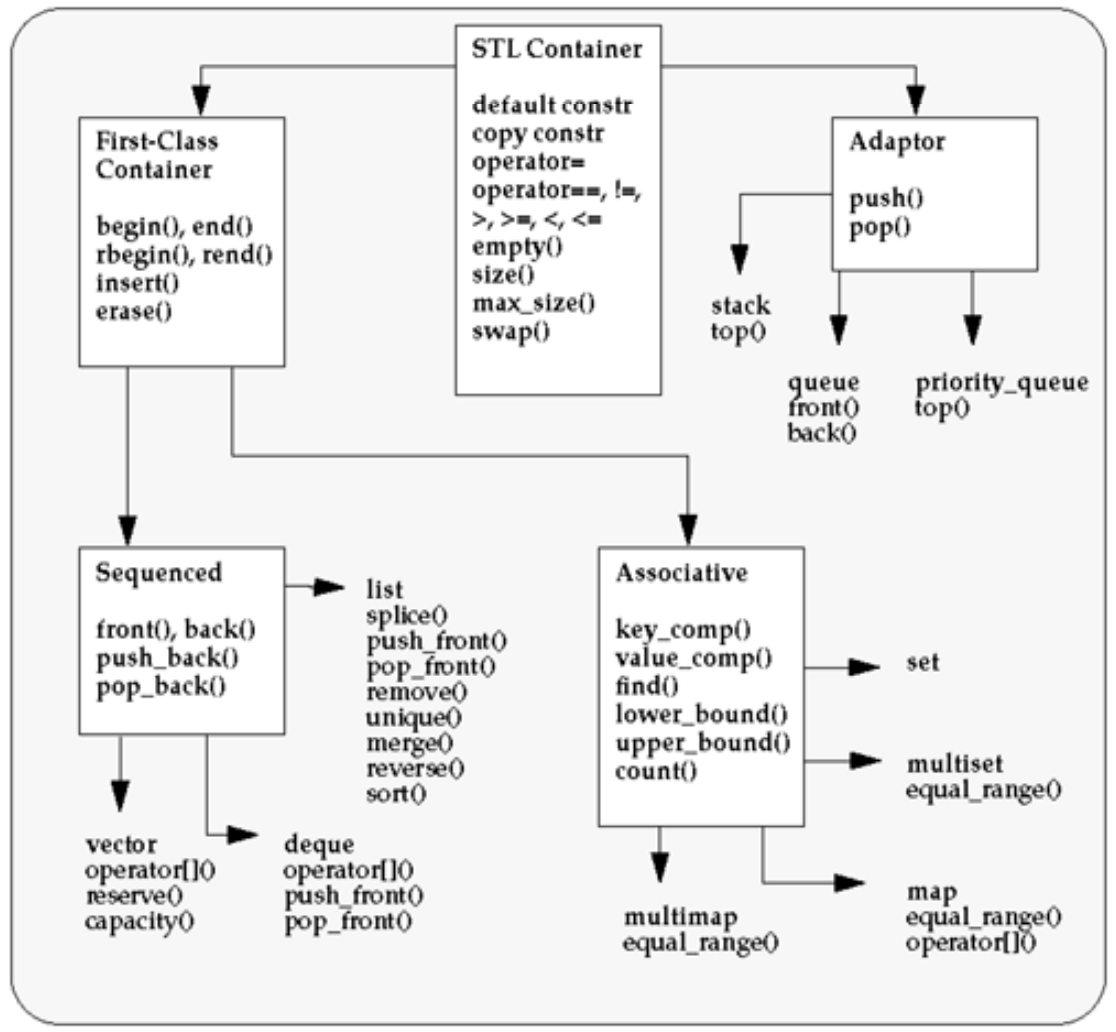
\includegraphics[scale=0.6]{pics/container.png}

\begin{enumerate}
\item  If you can find same name member functions in container, prefer to use member function than generic algorithm. Such as \textbf{sort, merge, remove, reverse, unique in list, and find, count, low\_bound in set and map. }




\item all container support empty(), size(), max\_size(), and swap(). max\_size() is just theoretic value. (4  functions)
\item First class container includes begin(), end(), rbegin(), rend(). insert() and erase(). (6 functions)
\item sequence container support pop\_back(), push\_back(),front() and back() (4 functions)
 while associative don't.
\item vector support operator[], list support push\_front and pop\_front. and deque support both. (3 function.)  By now deque support (4+6+4+3 = 17 functons)\textbf{container(4)--> first container(6)-->sequence container(4)-->deque(3)}
\item vector support reserve, list has reverse(\textbf{not reserve}) and splice().  deque support nothing.
\item list support it's own  version sort(), remove(), merge(),unique(). For other container, you can use the generic algorithm, Why list has its own? For sort(), list doesn't support random access iterator. For merge(), remove() and unique(). generic algorithm just use copy method, but list has high efficient pointer implementation, So list offer its own version merge(), remove(),sort(), unique().

\item All first class container support begin() and end(). Only sequence containers support push\_front() or push\_back(). \textbf{begin is not equal front, begin can be used for all first class container, but front only be used for sequence container.}

\begin{enumerate}
\item begin() and end() return iterator, and all first container support them.
\item front() and back() return reference, and all sequenced container support them.
\item push\_front() and push\_back() add element, and vector only support push\_back. deque and list support both.
\end{enumerate}


\item Associative container support It's own find(), count(),  lower\_bound(), upper\_bound() , equal\_range(). They share the same name with generic algorithm, Don't confuse them. When you deal with associative container, just use container member function, don't use generic algorithm. \textbf{Associative offer log-time lower\_bound, upper\_bound and equal\_range, but generic algorithm just linear time.}


\item deque is the data structure of choice when most insertions and deletions take place at the beginning or at the end of the sequence. It doesn't not guarantee continuity within memory, and higher constant factor cost than vector. Although both offer random access to elements and linear-time insertion and removal from middle of a sequence, the vector is faster.  In my evernote, you can see a implementation of deque.

\item difference between vector and deque:
\begin{enumerate}
\item vector has relocation problem,If vector has 1000, It probably need log(1000) = 10 times relocation. that is a little costly. On the contrary, deque just allocate a new place then insert pointer of new place to pointer map. It's relatively cheap.


\item Elements in a deque are not contiguous in memory; vector elements are guaranteed to be. So if you need to interact with a plain C library that needs contiguous arrays, or if you care (a lot) about spatial locality, then you might prefer vector.

\item For stack and queue default use deque as container inside. Why, because for a large amount of element, vector has relocation problem,
\end{enumerate}


\item All the container adapter support push(), pop(). and stack and priority\_queue support top(). They don't have any iterator.

\item If you want strongly error-safe code, such as transnational semantics for inserting and erasing, or need to minimize iterator invalidation, prefer a node-based container.

\item Using a vector for small list is almost always superior to using list. Even though inseriton in the middle of the sequence is a linear-time operation for vector and a constant-time operation for list. Vector usually outperforms list because of its better constant factor. \textbf{list's Big-Oh advantage doesn't kick in until data sizes get larger}

\item Store only values and smart pointers(unique\_ptr or shared\_ptr) in container.
\begin{enumerate}
\item To contain objects even though they are
not copyable or otherwise not value-like (e.g., DatabaseLocks and
TcpConnections), prefer containing them indirectly via smart pointers (e.g.,
container< shared\_ptr<DatabaseLock> > and container<shared\_ptr<TcpConnection> >).
\item Optional values. When you want a map<Thing, Widget>, but some
Things have no associated Widget, prefer map<Thing, shared\_ptr<Widget> >.
\item Index containers. To have a main container hold the objects and access them using different sort orders without resorting the main container, you can set up secondary containers that "point into" the main one and sort the secondary containers in different ways using dereferenced compare predicates. But prefer a container of MainContainer::iterators (which are value-like) instead of a container of pointers.

\item To have a container store and own objects of different but related types, such as types derived from a common Base class, prefer container< shared\_ptr<Base> >. An alternative is to store proxy objects whose nonvirtual functions pass through to corresponding virtual functions of the actual object.
\end{enumerate}

\end{enumerate}

\end{itemize}


\subsubsection{contiguous or node}

\begin{itemize}
\item Another classification of containter : contiguous-base and node-base.
\begin{enumerate}
\item vector, string, and deque
\item list and slist(linked list), set and map(balanced trees)
\end{enumerate}

\item Why we have this point of view.
\begin{enumerate}
\item \textbf{Because all the contiguous-base container has invalidation of iterator(pointer, reference) problem. }
\item \textbf{All the node-base container only support bidirectional iterators. }
\item \textbf{All the node-base container don't have reserve() function and need NOT to worry allocation problem. deque doesn't have reserve() function either }
\end{enumerate}

\item About the iterator invalidation problem,  First, you need to know the invalidation rules below:
\begin{description}
\item[Insertion]
\begin{itemize}
\item Sequence containers
		\begin{enumerate}
		\item vector: all iterators and references before the point of insertion are unaffected, unless the new container size is greater than the previous capacity (in which case all iterators and references are invalidated)
		\item deque: all iterators and references are invalidated, unless the inserted member is at an end (front or back) of the deque (in which case all iterators are invalidated, but references to elements are unaffected)
		\item list: all iterators and references unaffected
		\end{enumerate}

\item Associative containers: [multi]{set,map} all iterators and references unaffected

\item Container adaptors:  stack, queue and priority\_queue: inherited from underlying container.(Usually, we don't use iterator in stack, queue and priority\_queue. Maybe you don't need to worry about it. )
\end{itemize}

\begin{lstlisting}[frame=single, language=c++, mathescape=true]	
vecArr.insert ( it + 2, 1 , 200 );

// Reinitialize the invalidated iterator to the begining.
it = vecArr.begin();
\end{lstlisting}

\item[Erasure]
	\begin{itemize}
			\item Sequence containers
					\begin{enumerate}
					\item vector: every iterator and reference after the point of erase is invalidated
					\item deque: all iterators and references are invalidated, unless the erased members are at an end (front or back) of the deque (in which case only iterators and references to the erased members are invalidated)
					\item list: only the iterators and references to the erased element is invalidated
					\end{enumerate}
			
			\item Associative containers: [multi]{set,map}: only iterators and references to the erased elements are invalidated
			
			\item Container adaptors: stack, queue and priority\_queue: inherited from underlying container
	\end{itemize}

\begin{lstlisting}[frame=single, language=c++, mathescape=true]	
	 auto it = std::find(vecArr.begin(), vecArr.end(), 5);
    if(it != vecArr.end())
        vecArr.erase(it);
       $\Hilight{12}$it = vecArr.erase(it);

    // Now iterator 'it' is invalidated because it
    //  still points to old location, which has been deleted.
for(; it != vecArr.end(); it++)//Unpredicted Behavior
 std::cout<<(*it)<<"  "; //Unpredicted Behavior
\end{lstlisting}

\item[swap]
no swap() function invalidates any references, pointers, or iterators referring to the elements of the containers being swapped.

\item[Resizing]
vector, deque and list  as per insert/erase
\end{description}

\end{itemize}


\subsubsection{Search in Container}
\begin{itemize}
\item Distinguish among count, find, binary\_search, lower\_bound, upper\_bound, and equal\_range.

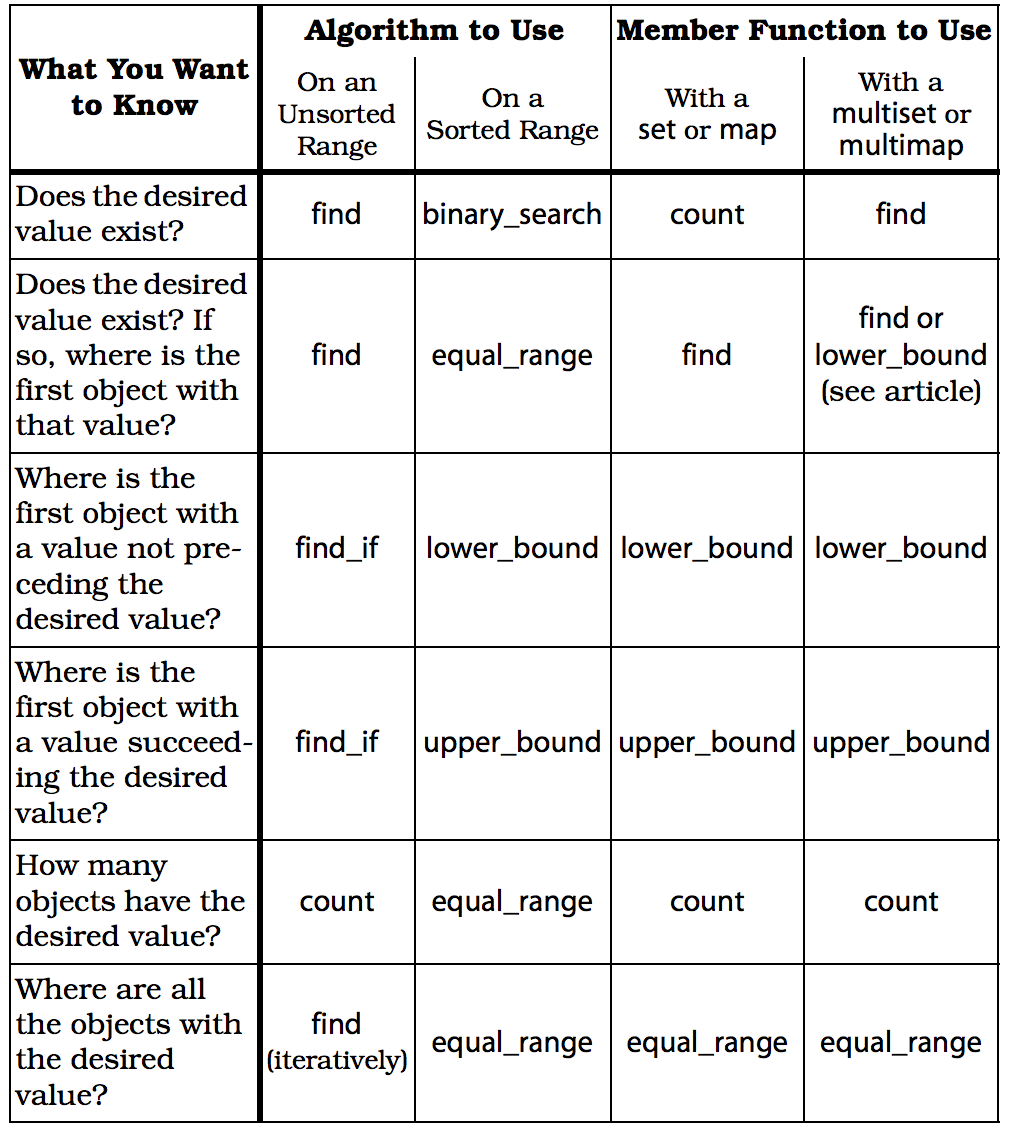
\includegraphics[scale=0.6]{pics/distinguish.png}

\begin{enumerate}
\item \textbf{For unsorted range, just generic find() or find\_if() algorithm or  count. return last if no find element.}
\item \textbf{For sorted range, Only four binary\_search, lower\_bound, upper\_bound, and equal\_range. are used on a sorted range.}
\item \textbf{For set or map, It has own version, find(),count() and lower\_bound, upper\_bound, and equal\_range}
\item Don't use generic find() algorithm on a sorted range,  use binary\_search(). binary\_search just return bool, not position.

\item  find() will return match iterator, if no match, it will return end()(for map or set). or last iterator(for generic algorithm). but Lower\_bound  will return a position anyway, match position or insert position(no match).

\item Lower bound: first element that is greater-or-equal. Upper bound: first element that is strictly greater. equal\_range return a pair of (lower\_bound, Upper\_bound).

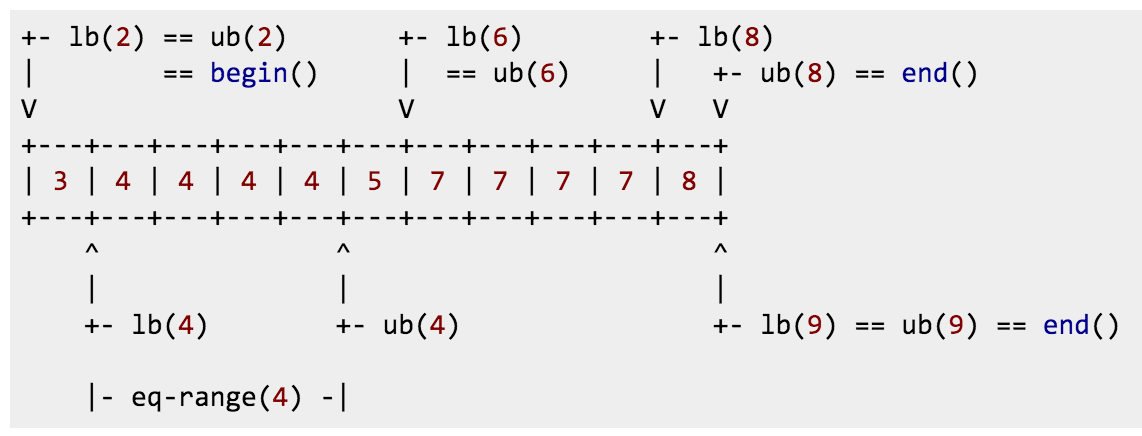
\includegraphics[scale=0.66]{pics/lowerupper.png}

\item equal\_range  if two iterators equal, (no found,). if two iterators distance >=1, (find one or more match, can replace find() or count() function.) .
\begin{lstlisting}[frame=single, language=c++]
  std::sort (v.begin(), v.end());
  // 10 10 10 20 20 20 30 30
 auto p =std::equal_range (v.begin(), v.end(), 20);
 for ( auto i = p.first; i != p.second; ++i )
        std::cout << i->name << ' ';

  //or code below:
  if(distance(p.first, p.second)  >=1){
       cout<<" found match"<<endl;
  }
\end{lstlisting}

\end{enumerate}
\end{itemize}


\subsubsection{Range}

\begin{itemize}

\item Copy algorithm usage: 1) copy v2 to v1.  2) it use loop inside.  \textbf{Almost all uses of copy where the destination range is specified using an insert iterator should be replaced with calls to range member function.}

\begin{lstlisting}[frame=single, language=c++]
v1.clear();
copy(v2.begin(), v2.end(), back_inserter(v1) );

//prefer to use below three range memeber function
v1.insert(v1.end(), v2.begin(),v2.end() );  //better than copy
v1.assign(v2.begin(), v2.end() )
// if want to replace all value in v1.
vector<int> v1( v2.begin(), v2.end() );
// build from sractch.
v1.erase( v1.begin(), v1.begin()+5);
//erage range.
\end{lstlisting}

\item A good example to explain why use range member function is below: When you use insert, inside of insert,  STL will get distance(n elements) of v2,begin() and v2.end(). Then , It will reserve and move the all element in v1 just once according to the distance.  If you use copy, it use loop insert one by one, It will move all element in v1 n times. if no space, it will reallocate and copy old element, just like common vector do. So use range member function, can save you a lot of time in this example.

\begin{lstlisting}[frame=single, language=c++]
//don't use front_inserter() here,
//because vector don't support push_front()
copy(v2,begin() , v2.end(),
          inserter(v, v.begin() ) );

// a better method is here.
v1.insert(v1.begin(),  v2,begin() , v2.end());
\end{lstlisting}

\item effective STL Item 5: Prefer range member functions to their single-element counterparts.
\begin{enumerate}
\item Range construction:
\item Range insertion:
\item Range erasure:
\item Range assignment:
\end{enumerate}

\begin{lstlisting}[frame=single, language=c++]
container::container(inputIterator1, inputIterator2);
container::insert(insertPosition, inputIt1, inputIt2);
container::erase(inputIterator1, inputIterator2);
container::assign(inputIterator1, inputIterator2);
\end{lstlisting}


\item The main reason for using assign is to copy data from one type of container to another.
\begin{enumerate}
\item For example, if you want to migrate the contents of an std::set<int> to an std::vector<int>, you can't use the assignment operator, but you can use vector.assign(set.begin(), set.end()).

\item Another example would be copying the contents of two containers holding different types that are convertible to one or the other; If you try to assign std::vector<Derived*> to an std::vector<Base*>, the assignment operator is insufficient.
\item different part from one container to another.
\end{enumerate}



\end{itemize}

\subsubsection{Erasure}
\begin{itemize}


\item So, in short: generally speaking, you should not delete the items from the list while iterating through it, because the deletion may invalidate the iterator (and the program will possibly crash). If you are however completely sure that the items which you delete are not the values referenced by any of the iterators which you use at the moment of deletion, you may delete.

\item Beware that for the other STL containers (e.g. vectors) the constraint is even more strict: deleting from the container invalidates not only iterators pointing to the deleted item, but possibly other iterators, too! So deleting from that containers while iterating through them is even more problematic.

\item Choose carefully among erasing options:  To eliminate all objects in a container that have a particular value.
\begin{enumerate}
\item For vector, string or deque, use erase-remove. \textbf{Don't use for loop, it will invalid the iterator.}
\item For a list, use it's own remove or remove\_if.
\item For associative container, use its erase member function.
\end{enumerate}

\begin{lstlisting}[frame=single, language=c++]
vect.erase(remove(vect.begin(), vect.end(),1963), vect.end());
list.remove(1963);
map.erase(1963);
\end{lstlisting}

\item  To eliminate all objects in a container that satisfy a particular predicate, 1)for vector, string or deque, use erase-remove. 2) for a list, use remove\_if, 3) for associative container, write loop being sure to postincrement your iterator. detail can be sen in effective STL item 9;
\begin{lstlisting}[frame=single, language=c++]
bool badValue(int x);
vc.erase(remove(vc.begin(), vc.end(), badValue),
                                          vc.end());

lsit.remove_if(badValue);
for(auto i = map.begin();i!=map.end(); /* no ++i here*/) {
	if(badVaue(*i)) map.erase(i++);
	// or i = map.erase(i);
	else  ++i;
}
\end{lstlisting}

\item  To do something inside the loop (in addition to erasing objects);  You can't use remove, just write a loop,
\begin{lstlisting}[frame=single, language=c++]
bool badValue(int x);
for(vect<int>::iterator i = vect.begin();i!=vect.end(); ){
	if(badVaue(*i)) {
		i = vect.erase(i);
		...do something else
	}
	else  ++i;
}
\end{lstlisting}

\end{itemize}
\subsubsection{value\_type in container}
\begin{itemize}
\item value\_type in container.
\begin{lstlisting}[frame=single, language=c++]
vector<uint> vecs;
cout << sizeof(vecs.value_type)  //error usage
cout<<sizeof(vector<uint>::value_type);
//Pay attention to :: because it's static class member.
\end{lstlisting}

\item Having the commonly-used types available as a type on the container is useful when the container's type itself is unknown. For example, someone may want to write library code that works equally well with std::map and std::unordered\_map:
\begin{lstlisting}[frame=single, language=c++]
template<typename TMap>
void insert_default_pair(TMap& map)
{
    map.emplace(typename TMap::key_type(),
                       typename TMap::mapped_type());
}
share
\end{lstlisting}

\item inside templated code, prefix value\_type with the keyword typename. Why, It depending on whether some identifier designates a type or a variable, e.g.T * p may be a multiplication or a pointer declaration. Not explicitly marked as type by prefixing it with typename is considered a variable.

\begin{lstlisting}[frame=single, language=c++, mathescape=true]
template <typename T>
class TSContainer {
private:
        T container;
public:
        void push($\Hilight{5}$typename T::value_type& item){
                container.push_back(item);
        }
\end{lstlisting}


\item summary:
\begin{enumerate}
\item complex type
\item change a lot, in above example
\item Inside of a function
\item previous two example, unknow container in template class or support two container at the same time, to reach generic purpose.
\end{enumerate}
\begin{lstlisting}[frame=single, language=c++, mathescape=true]
//1)it will save a lot of typing.
 typedef vector< pair<int, string> > ComVec;
ComVec::value_type aaa;

//2)int to float, but below code don't need change at all.
typedef vector< pair<float, string> > ComVec;

//3) inside of funciton.
typedef std::vector< std::pair<int,std::string> > Record_t;
//$\Hilight{28}$ typedef is your good friend, reuse it below
Record_t k1;

int find_it(std::string value, $\Hilight{6}$Record_t const& stuff){
  auto fit = std::find_if(stuff.begin(), stuff.end(),
            [value]($\Hilight{14}$Record_t::value_type const& vt) -> bool
                 { return vt.second == value; });
\end{lstlisting}

\end{itemize}


\subsubsection{Sizes}
\begin{itemize}
\item For container, Call empty() instead of of checking size() against zero. it's very easy to understand it.

\item for vector, size(), capacity() and max\_size() can be seen below: capacity is equal or bigger than size. So if you want to avoid allocate the unnecessary space.  LLVM give a SmallVecotr<type, N> example, you can use N to specify a smaller vector to avoid waste.
\begin{lstlisting}[frame=single, language=c++]
std::vector<int> myvector;
for (int i=0; i<100; i++) myvector.push_back(i);

std::cout << (int) myvector.size() << '\n'; // 100
std::cout  << (int) myvector.capacity() << '\n';  //128
std::cout << (int) myvector.max_size() << '\n';  //1073741823
\end{lstlisting}


\item Four confused conceptions:
\begin{lstlisting}[frame=single, language=c++]
capacity() //how many CAN hold
size()   //how many are in NOW
resize(n) // forces the container to change to n,
//if n <size(),  object in the end will be lost
// if n>size(),  default ctor of element will be called.
// after resize(n), size will return n.
// but resize don't change capacity

reserve(n) //cause the container's capacity() to at lease n.
\end{lstlisting}

\item You want to avoid allocation, 1), if you know the number, then use reserve, 2) if you don't know the number, you can reserve maximum space, then you can trim off any excess capaciy.  you can use shrink\_to\_fit() function too. Just remember \textbf{string(s).swap(s)}
\begin{lstlisting}[frame=single, language=c++]
vector<class> v1;
v1.reserve(1000); v1.size(); // only 5

vector<class>(v1).swap(v1);
//1) vector<class>(v1) copy ctor create a temp vector
//2) temp just copy real object, so it's capacity (maybe 8)is small.
//3) temp.swap(v1) then temp has 1000 space,  v1 capacity is 8 now
//4) in the end of statment, temp destory.
string(s).swap(s) // the same idea behind.
\end{lstlisting}

\item Worthwhile note about vector: It will avoid allocate new space many times.
\begin{lstlisting}[frame=single, language=c++]
std::vector<int> v
for(){ ...
 v.clear
}  //good smell.

for(){vector<int> v ...} //bad smell
\end{lstlisting}
\item resize and reserve difference.
\begin{lstlisting}[frame=single, language=c++]
vector<Foo> vcFoo;
vcFoo.reserve(10);
vcFoo.resize(10); // will call Foo ctor 10 times
vcFoo[2] = foo; // will call Foo ctor and assignment 1 times
// if no reserve or resize. vcFoo[2] = foo will fail.
\end{lstlisting}


\end{itemize}

\subsubsection{Usages Tips}
\begin{itemize}

\item \textbf{When you use STL Container, you should realize that typedef are your best friends.}
\begin{lstlisting}[frame=single, language=c++]
typedef vector<Foo, SpecialAllocator<Foo> > FooContainer;
typedef FooContainer::iterator FooIt;

FooContainer fc1; // make you programming more clearly,
FooContainer fc2;  // you should use typedef more
FooIt it1;
\end{lstlisting}


\item Never try to expect all the container has the same interface. Even a generic erase(), for sequence, It return next iterator,(because it will invalid the iterator).   But for associative, it return void(c++ 98) and return next iterator(C++ 11). If you just want to change a container in the future, you should put a container into a class: CustomCollection. then hide it from the class client. The detail can be seen in Effective STL item 2.

\item The standard associative container are implemented as balanced binary search trees.  It's optimized for a mixed combination of insertions, erasures and lookup.  But if that is dictionary, It can be fall into three distinct phases. setup, lookup, modify. and modify is not happen very often. lookup is very often. At this time, associative container is not best option. sorted vector also support log search time.  1) It use less space. 2) more space cause page fault in memory, then the same log search complex, but sorted vector is faster than associate container.\textbf{ For dictionary, please use sorted vector.}


\item Avoid using vector<bool>, use deque<bool> or bitset


\item item 22 Avoid in-place key modification in set and multiset
\begin{enumerate}
   \item you can't change key in map because it's const default.
\begin{lstlisting}[frame=single, language=c++]
map.begin()->fist = 10 //compile error
\end{lstlisting}

   \item For set or map, you can modify non-key part.
\begin{lstlisting}[frame=single, language=c++]
iterator i = set.find(employee);
if( i != set.end())
   i->setTitle("manager")  // it's also ok or
   const_cast<Employee &> (*i).setTitle("manager")
   // you must change it to a reference, then you can modify it.
   // if you just use  const_cast<Employee >
   // this is not right. it will create a temporary obj
   //and then modify a temporary obj.
\end{lstlisting}

\item If you want to modify the key part in set or map.
\begin{lstlisting}[frame=single, language=c++]
 // 1) find the one
 iterator i = se.find(employee);
 //2) create temp one.
 if(i ! = se.end())
 Employee e(*i);
 //3) modify
 e.setKey("new key")
 //4) delete the old one and keep ;
  se.erase(i++);
  //5) insert new one
  se.insert(i,e);
\end{lstlisting}
    \end{enumerate}

\item Item19 effective STL, Understand the difference between equality and equivalence in associative Containers.
  \begin{enumerate}
  \item equality is based on operator ==. equivalence is based on operator<. Because associate container, set, map, they must sort their elements, so they must use operator<. Then it use !if(a<b)\&\&!if(b<a) to define equivalence, and associate container use equivalence to decide if a object exist in container.
  \item if you don't have custom compare funciton, most of time equivalence is equal to equality, but if you define you specific compare function, you need to know below:
  \item It will cause container.find and generic algorithm find has different result
\begin{lstlisting}[frame=single, language=c++]
 set<string,  case_insensitive_compare> ss;
 //ss has "AA";
 ss.find("aa"); //return true;
 find(ss.begin(),ss.end(),"aa") //return false
 //find algorithm use operator == .
\end{lstlisting}
  \item It will lead to item 21 in effective STL. Always have comparison functions return false for equal values. (strict weak ordering )
  \item It will lead to item 20 in effective STL. For associative container of pointers, You need to specify comaprsion types, You want to order by pointers or want to order by objects pointed by pointer.(Most of time, the second option is what we want)
\begin{lstlisting}[frame=single, language=c++]
struct stringLess: binary_fucntion<const string* ,
                         const string * , bool>{
   bool operator()(const string* s1 ,
                            const string * s2){
        return *s1<*s2;
}
}
 set<*string,  stringLess> ss;
\end{lstlisting}


  \end{enumerate}

\end{itemize}

\subsubsection{string}
\begin{itemize}
\item String::npos is the maximum possible length of the string. Equal the maximum value of an unsigned int.
\item String is template specialization basic\_string<char> , from this point of view, you will know how to construct a w\_char string.
\item There are a lot of ways that can be used construct a string object, you can see the reference , such as:
\begin{lstlisting}[frame=single, language=c++]
string(const char* s);
 string(const char*, size_type n);
 string(const string& str, size_type pos, size_type n = npos)
 ......
\end{lstlisting}

\item The standard containers define size\_type as a typedef to Allocator::size\_type (Allocator is a template parameter), which for std::allocator is defined to be size\_t. So for the standard case, they are the same. However, if you use a custom allocator a different underlying type could be used. So container::size\_type is preferable for maximum portability.

\item In C++, we encourage you to use string more, to replace char[] and char *p = new.  Because it offer you more functions, such as\textbf{ compare, find,erase, replace,insert}.

\item About real size of string, string usually manage it's memory by itself, but you can use two functions string::capacity() and string::reserve() to do some simple work. If the size of string is not enough, string will allocates a new block twice the size and copy the old content. You can use capacity to know the real block size. And use reserve to tell string at least you need minimum size of bloc. For example, str.reserve(50),  str.capacity will return 63. 63 = 64-1; string need the last char to store \verb='\n'= and end of symbol.

\item When you use string with some legacy c function, use string.c\_str() function for read only function, string.c\_str() return a const char *. so You can't modify it. If you Legacy C function want to fill in a string. you need do below:

\begin{lstlisting}[frame=single, language=c++]
Old_c(const char* p); string str;
Old_c(str.c_str());  // legacy C function read a string

// legacy C write
size_t Old_c(char *pArray, size_t arraySize);

vector<char> vc(maxNumChars);
// 1) create a vector whose size is maxNumChars
size_t charsWritten = Old_c(&vc[0], vc.size());
// 2) have fillString write into vc
string s(vc.begin(), vc.begin()+charsWritten);
// 3) copy data from vc to s via range constructor
\end{lstlisting}

\item string method lists:

\begin{tabular}{| p{0.3\textwidth} |p{0.7\textwidth}|}
\hline
capacity(), reserve() & Returns the largest number of elements that could be stored in a string without increasing the memory allocation of the string.\\
\hline
empty(),  size()& \\
\hline
max\_size() & maximum number of characters \\
 resize() & Specifies a new size for a string, appending or erasing elements as required.\\
\hline
 length() & Returns the current number of elements in a string.\\
\hline

\end{tabular}

\begin{tabular}{| p{0.3\textwidth} |p{0.7\textwidth}|}
\hline
find(), rfind() & Searches a string in a forward/backward direction for the first occurrence of a substring that matches a specified sequence of characters.\\
\hline
substr() & Copies a substring of at most some number of characters from a string beginning from a specified position. \\

\hline
find\_first\_not\_of() & Searches through a string for the first character that is not any element of a specified string.\\
\hline
find\_first\_of() & \\
\hline
find\_last\_not\_of() & \\
\hline
find\_last\_of() & .\\
\hline
\end{tabular}

\item find function in the string return position. Vector doesn't have find member function, you can use find function in  algorithm category.

\begin{lstlisting}[frame=single, language=c++]
size_t found;
found=str.find("haystack");
// or found=str.find('.');
if (found!=std::string::npos)
    std::cout << "'haystack' also found at: " << found << '\n';

vector<int> myints = { 10, 20, 30, 40 };
auto  it = std::find (myints.begin(), myints.end(), 30);
if(it!=myints.end())
   cout<< "find 30"<<endl;
\end{lstlisting}


\begin{tabular}{| p{0.23\textwidth} |p{0.77\textwidth}|}
\hline
begin(),end() & Returns an iterator addressing the first element in the string.\\
\hline
rbegin(), rend() & \\
\hline

\end{tabular}


\begin{tabular}{| p{0.25\textwidth} |p{0.75\textwidth}|}
\hline
clear()& Erases all elements of a string.\\
\hline
insert(), erase() & Inserts an element or a number of elements or a range of elements into the string at a specified position.\\
\hline
append(), push\_back() & Adds characters to the end of a string.\\
\hline
assign() &Assigns new character values to the contents of a string.\\
\hline
replace() & \\
\hline
\end{tabular}

\begin{tabular}{| p{0.25\textwidth} |p{0.75\textwidth}|}

\hline
at() & a reference to the element at a specified location \\
\hline
c\_str(), data() & \\
\hline
compare()& \\
\hline
copy() & Copies at most a specified number of characters from an indexed position in a source string to a target character array.The function does not append a null character at the end of the copied content.
\\
\hline
get\_allocator() & Returns a copy of the allocator object used to construct the string.\\
\hline


\hline
swap() & Exchange the contents of two strings. \\
\hline
\end{tabular}

\item clear will delete all the characers, and erase will remove character in certain position.

\item position in find method can be used in loop
\begin{lstlisting}[frame=single, language=c++]
std::string str ("Please, replace the vowels with asterisks.");
  std::size_t found = str.find_first_of("aeiou");
  while (found!=std::string::npos)
  {
    str[found]='*';
    found=str.find_first_of("aeiou",found+1);
  }
\end{lstlisting}


\end{itemize}


\subsection{Iterator}

\begin{itemize}
\item There are 5 classification iterators: input, output, forward, bi-direction, random. You need to know these five are not real class, they are just conception, not real implementation.

\item As mentioned earlier, each container class defines a class scope typedef name called iterator. So the vector<int> class has iterators of type vector<int>::iterator.  The document will tell you vector iterators is  random access iterators.

 \item In practical point of view: There are four points you need to know:
\begin{enumerate}
\item Five classification and associated supported operation.
\item Common container's iterator classification.
\item Common algorithm can accept what kind of iterator. (See next chapter)
\item Use typedef simply define container iterator.(typedef is good friend when you use stl more and more);
\end{enumerate}

\item Now, five classification iterators play important role here: From this figure, you can know what operation each iterator supports.  \newline

  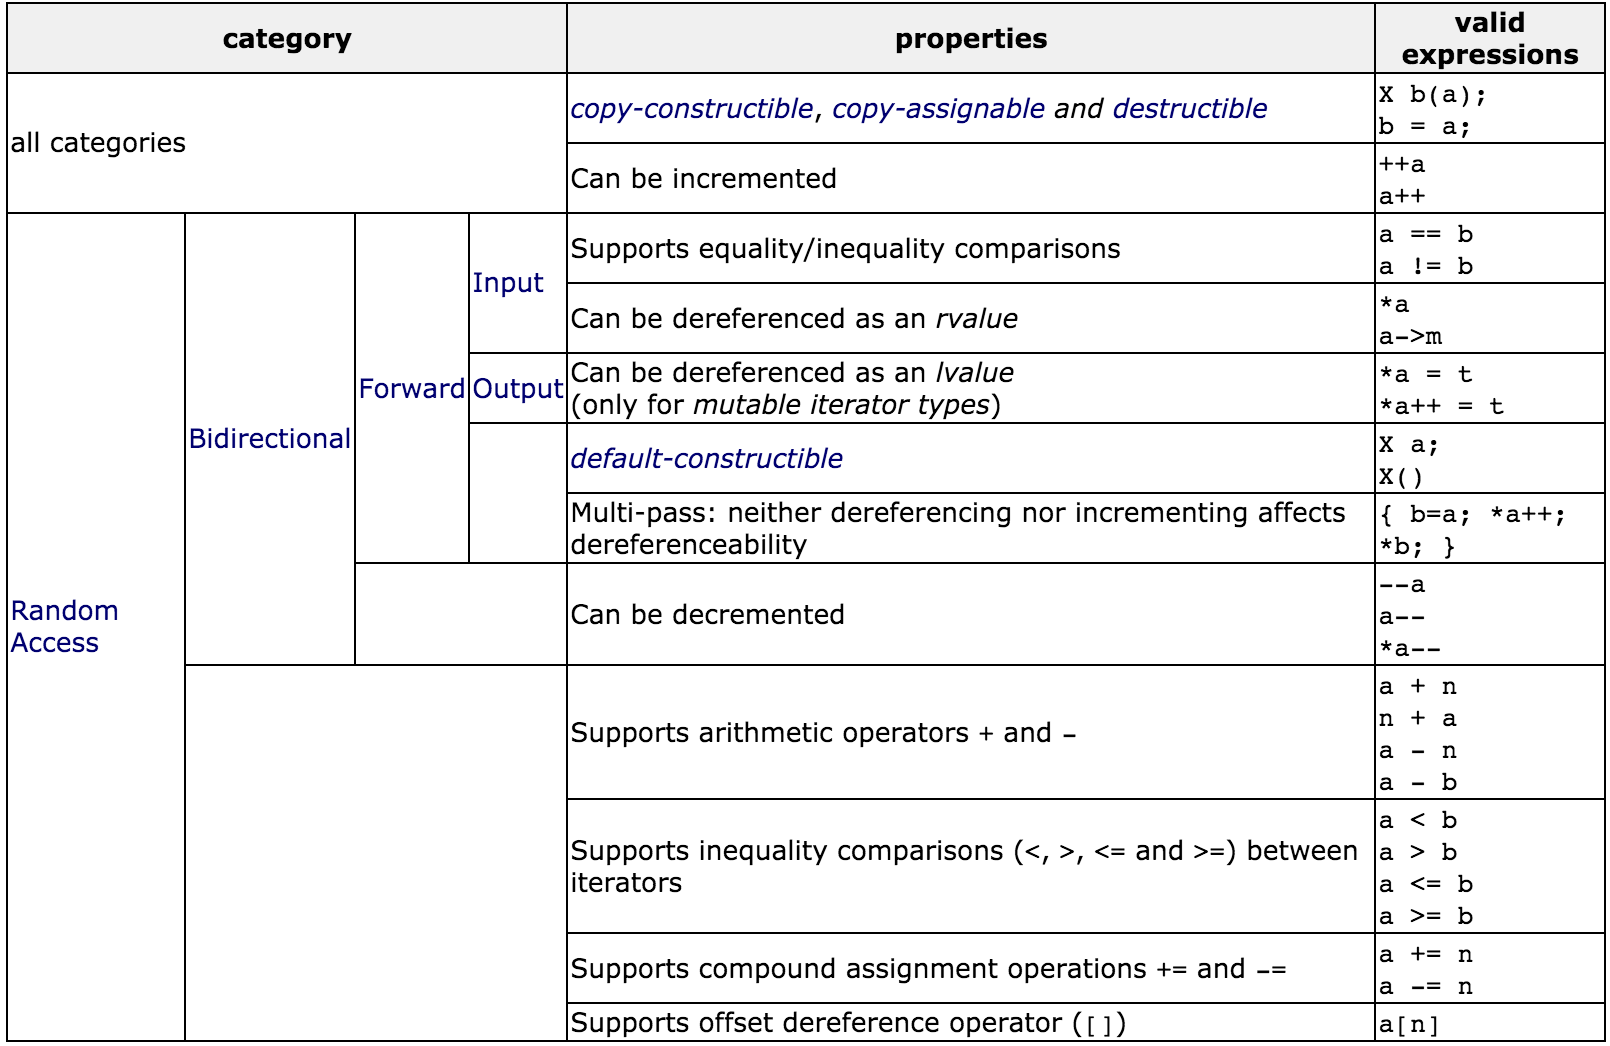
\includegraphics[scale=0.48]{pics/iterator.png}

\item Basic container iterator is below: \newline

  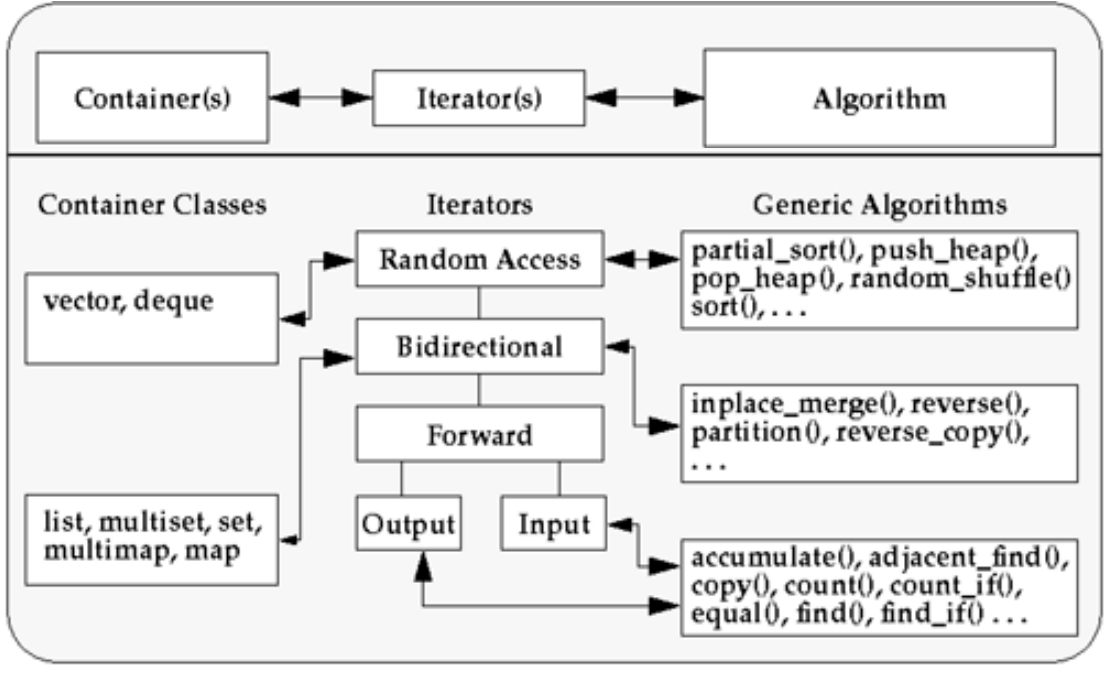
\includegraphics[scale=0.56]{pics/container_it.png}

\item In each container, iterator of container is implemented by itself. There is no iterator class inheritance hierarchical structure.  I means that in vector, there is vectIter: Iterator (vectIter inheriate from base iterator class) , then you define ++ operator in class vectIter class. It's totally wrong. In fact, In vector, Maybe iterator is defined by:
\begin{lstlisting}[frame=single, language=c++]
template<type T>
vector{
....
typedef T* iterator;
};

vector<int>::iterator ip; //use it outside.
// ++ and -- is done by pointer automatically.
\end{lstlisting}

and All the member function of vector know the iterator very well, inside, it will use T* directly,
\begin{lstlisting}[frame=single, language=c++]
push_back(T x){
*end++ = x;
}  // you can see there is no iterator
   // when you implement container implementation.
\end{lstlisting}


\item When you see the algorithm,  you will see the algorithm is based on template, not inheritance. (You don't need to make type can be cast or not. ). \textbf{Algorithm don't care what iterator really is, It just make sure each iterator can support what operation. }
\begin{lstlisting}[frame=single, language=c++]
template <class InputIterator, class OutputIterator>
  OutputIterator copy (InputIterator first, InputIterator last,
            OutputIterator result);
\end{lstlisting}


\item Common four iterator errors.
\begin{enumerate}
\item Valid values: Is the iterator dereferenceable? For example, writing "*e.end()" is always a programming error.
\item Valid lifetimes: Is the iterator still valid when it's being used? Or has it been invalidated by some
operation since we obtained it?

\item Valid ranges: Is a pair of iterators a valid range? Is first really before (or equal to) last? Do
both really point into the same container?
\item Illegal builtin manipulation: For example, is the code trying to modify a temporary of builtin
type, as in "--e.end()" above? (Fortunately, the compiler can often catch this kind of mistake
for you, and for iterators of class type, the library author will often choose to allow this sort of
thing for syntactic convenience.)


\end{enumerate}


\begin{lstlisting}[frame=single, language=c++]
int main(){
vector<Date> e;
copy( istream_iterator<Date>( cin ), istream_iterator<Date>(), back_inserter( e ) );
vector<Date>::iterator first = find( e.begin(), e.end(), "01/01/95" );
vector<Date>::iterator last = find( e.begin(), e.end(), "12/31/95" );
*last = "12/30/95";
copy( first, last, ostream_iterator<Date>( cout, "\n" ) );
e.insert( --e.end(), TodaysDate() );
copy( first, last, ostream_iterator<Date>( cout, "\n" ) );
}
\end{lstlisting}


\item You can inheriate you own iterator from std::iterator: yes, that's what it's for.If you mean anything else: no, because none of the STL iterators have virtual destructors. They're not meant for inheritance and a class inheriting from them might not clean up properly. a Good example can be seen link:  http://www.cplusplus.com/reference/iterator/iterator/

\item two common iterator operation:  advance() and distance().
\begin{lstlisting}[frame=single, language=c++]
std::list<int>::iterator first = mylist.begin();
std::list<int>::iterator last = mylist.end();

std::advance(first, 3) //
std::cout  << std::distance(first,last)
\end{lstlisting}


\item istream\_iterator and istreambuf\_iterator topic:
\begin{lstlisting}[frame=single, language=c++]
 std::ostream_iterator<int> out_it (std::cout,", ");
 std::copy ( myvector.begin(), myvector.end(), out_it );

 ifstream inputFile("aa.txt");
 string fileData((istreambuf_iterator<char>(inputFile)) ,
  istreambuf_iterator<char>());
// It will just read all the character.(including white character)
// I don't need format data,

 ifstream inputFile("aa.dat");
 list<int> data((istreambuf_iterator<char>(inputFile)) ,
  istreambuf_iterator<char>());
 // It wil  read format data, and use white space as delimiter.
\end{lstlisting}

\end{itemize}

\subsubsection{Insert iterator}
\begin{itemize}
\item Three common iterator generator: inserter(), back\_inserter(), front\_inserter();  They will produces three insert\_iterator: insert\_iterator, back\_insert\_iterator and front\_insert\_iterator.

\item When you use insert\_iterator in an assignment, insert\_iterator will call insert() function.  back\_insert\_iterator will call push\_back() and front\_insert\_iterator will call push\_front(). insert\_iterator++ has no any operator inside.

\item  std::inserter is commonly used with sets

\item Why do we need it. in some algorithm, such as copy and generator, if you read sth from a container, you can use regular iterator, but when you want to write into a container.  You must keep regular iterator is valid. so a method is to use reverse before you write to a container.

\begin{lstlisting}[frame=single, language=c++]
list<State> res2( src.size() );
copy( src.begin(), src.end(),
    res2.begin() ); // often works...
\end{lstlisting}

\item Another way is to use back\_insert\_iterator.
\begin{lstlisting}[frame=single, language=c++]
std::vector<int> foo;
for (int i=1; i<=5; i++)
  { foo.push_back(i); bar.push_back(i*10); }
  std::copy (bar.begin(),bar.end(),back_inserter(foo));
  //foo support push_back

  std::deque<int> foo;
  // deque or list
  for (int i=1; i<=5; i++)
  { foo.push_back(i); bar.push_back(i*10); }
  std::copy (bar.begin(),bar.end(),front_inserter(foo));
  //foo support push_front
\end{lstlisting}

\item Of course, you can use the random access iterators (or any output iterator) in algorithms like std::copy, as third argument, but that assumes the iterator is referencing to existing range — *it and ++it are well-defined for the value you passed. You pass them to overwrite the existing elements of the range, whereas std::back\_insert\_iterator adds new elements to the container.

\item For copy algorithm, pass vect.end() is not meanful, because It's not a valid iterator to support *it = new\_obj.

\end{itemize}


\subsubsection{Reverse iterator}
\begin{itemize}
\item reverse\_iterator topic:
You need a front-to-back traversal or a back-to-front traversal. The reason for reverse iterators is that the standard algorithms do not know how to iterate over a collection backwards. For example:
\begin{lstlisting}[frame=single, language=c++]
std::find(foo.begin(), foo.end(), L'a');
                  // Returns an iterator pointing
                      // to the first a character.
std::find(foo.rbegin(), foo.rend(), L'a').base()-1;
                      //Returns an iterator
                       // pointing to the last A.
std::find(foo.end(), foo.begin(), L'a');
                   //WRONG!! (Buffer overrun)
\end{lstlisting}

\item reverse\_iterator can use base() to change a normal iterator, because all the contain member function just receive normal iterator. such as insert and erase.
why ri.base() and ri will have step 1 advance. detail can be seen effective stl item 28.
\begin{lstlisting}[frame=single, language=c++]
reverse_iterator ri =
    find(foo.rbegin(), foo.rend(), L'a');
foo.insert(ri.base()); // you can use ri.base() directly.
                               // when you want to insert.
foo.erase((++ri).base()); //you can't use ri.base() directly.
                                 //when you erase what you want.
      ri
1 2 3 4 5
        i = ri.base()
\end{lstlisting}



\end{itemize}

\subsection{Algorithms}

\subsubsection{Basic}

\begin{itemize}

\item Effective STL item 43, \textbf{Prefer algorithm calls to hand-written loops}.
\begin{enumerate}
\item  Handing writing is prone to bug

\begin{lstlisting}[frame=single, language=c++]
for( size_t i = 0; i < max; ++i )
d.insert( current++, data[i] + 41 ); // do you see the bug?
\end{lstlisting}
\item You can fix it bu with careful design
\begin{lstlisting}[frame=single, language=c++]
for( size_t i = 0; i < max; ++i ) {
current = d.insert( current, data[i] + 41 ); // be careful to
keep current valid…
++current; // … then increment
it when it's safe
}
\end{lstlisting}
\item but a better way is
\begin{lstlisting}[frame=single, language=c++]
transform( data, data + max, // copy elements from data
inserter(d, d.begin()), // to the front of
\end{lstlisting}

\item With a complex algorithem, just use STL alogrithem+lambda
\item but a better way is
\begin{lstlisting}[frame=single, language=c++]
for( vector<int>::iterator i = v.begin(); i != v.end(); ++i )
if( *i > x && *i < y ) break;

// This is better version now.
vector<int>::iterator i = find_if( v.begin(), v.end(), [x, y](int &i){i>x && i<y} );
\end{lstlisting}



\end{enumerate}
But if you need a loop that dees something fairly simpler, but would require a confusing tangle of binders and adapters, just use loop.
\begin{lstlisting}[frame=single, language=c++]
list<Widget> lw;
type list<Widget>::iterator WI;
for_each(lw.begin(),lw.end(),
                mem_fun_ref(&Widget::redraw) );

transform(data, data+10, inserter(deque, deque.begin()),
        bind2nd(plus<double>(), 41));
\end{lstlisting}

\item There are four groups: non modifying sequence , mutating sequence, sorting, generalized numeric operations. Detail can be see c++ primer p1286.

\item Note which algorithm expect sorted ranges:
\begin{lstlisting}[frame=single, language=c++]
binary_search lower_bound upper_bound equal_range
set_union set_intersection set_difference
merge  inplace_merge  includes
unique  unique_copy
\end{lstlisting}



\item Make sure destination ranges are big enough effective stl item 30
\begin{lstlisting}[frame=single, language=c++]
vector<int> values, result;
int doSth(int x); // function
// make destination range big enough
result.reserve(result.size()+values.size() );

transform(values.begin(), values,end(), result.end(),doSth );
// It's error. transform writes its result by making
//assignment. result.end() has no object at all

transform(values.begin(), values,end(),
  back_inserter(result), doSth)  //insert end

transform(values.rbegin(), values,rend(),
  front_insert(result), doSth)
  //result must be a list
  // use rbegin make insert in front right order
\end{lstlisting}



\item Know you sorting options: It makes no sense to sort elements in standard associative containers, because such containers use their comparison functions to remain sorted all the time.

\item For other sequence container, sorting options is below: (1-3) need random iterator. 4 only need bidirection iterator.(list)
  \begin{enumerate}
  \item full sort on vector, string, deque, or array.  use sort or stable\_sort
  \item put only the top n elements in order, partial\_sort
  \item Identify the elements at position n , you need nth\_element
  \item spearate the elements of a standard sequence container, do satisfy some criterion, you use partition or stable\_partition.
  \item for list, you should use list.sort() in place of common sort.
  \end{enumerate}
\begin{lstlisting}[frame=single, language=c++]
vector<Foo> vf;
bool compare(const Foo& f1, constFoo& f2);
partial_sort(vf.begin(),vf.begin()+20, vf.end(),  compare);
sort(vf.begin(),vf.end(), compare);
nth_element(vf.begin(),vf.begin()+20,vf.end(), compare);

bool good(const Foo &f1)
partition(vf.begin(), vf.end(), good);
\end{lstlisting}

\item Be wary of remove-like algorithm on container of pointers
\begin{lstlisting}[frame=single, language=c++]
void delAndNULL(Foo*& pf){ // use pointer reference here.
if(!pf->isCertified(){ delete pf; pf = nullptr}
}
for_each(v.begin(),v.end(), delAndNULL);
v.erase(remove(v.begin(),v.end(),
                 static_cast<Foo *>(0) ), v.end());
\end{lstlisting}


\item \textbf{For a algorithms, you need to know three points: 1) what's function  for 2) what iterator it accept, 3) what functor it will accept.  So please see below summary. }
\end{itemize}

\subsubsection{basic notation}



Iterator:  \\
\begin{tabular}{| p{0.2\textwidth} |p{0.8\textwidth}|}
\hline b, f &	a bidirectional, forward iterator \\
\hline i,o,a 	&an input, output, random iterator  \\
\hline(?, ?)	&a pair of iterators as a return value, as in (f,f)  \\
\hline
\end{tabular}

functor:  \\
\begin{tabular}{| p{0.2\textwidth} |p{0.8\textwidth}|}
\hline upred, bpred	& a unary or binary predicate (boolean function or function object)
(generally used to test a single value from a container) \\

\hline ufunc, bfunc	&  a unary or binary  (value-returning) function or functor \\
\hline pfunc	& a "parameterless" (value-returning) function (or function object)
(often used to "generate" a value of some kind) \\
\hline uproc, bproc	& a unary or binary  procedure (void function or function object) \\
\hline pproc	&  a "parameterless" procedure (void function or functor) \\
\hline
\end{tabular}

Parameter:  \\
\begin{tabular}{| p{0.2\textwidth} |p{0.8\textwidth}|}
\hline n, v, \&  & 	a quantity (or size). A value. reference to a value \\
\hline
\end{tabular}

\subsubsection{Applying}
\begin{tabular}{| p{0.35\textwidth} |p{0.45\textwidth}|p{0.2\textwidth}|}
\hline ufunc for\_each(i,i,ufunc) &Apply a function to every item in a range and return the function. &  ufunc may not return value.  \\
\hline
\end{tabular}

\begin{lstlisting}[frame=single, language=c++, mathescape=true]
void fun(int n){
    cout<<" "<<n;
} $\Hilight{28}$//all function definition end no semicolon

struct Sum{
    Sum(): sumEven{0} { }  $\Hilight{15}$//no semicolon here
    void operator()(int n) { if(n%2 ==0) ; sumEven += n; }
    int sumEven;
}; $\Hilight{20}$// type definition need semicolon

vector<int> nums{3, 4, 2, 8, 15, 267};
for_each(nums.begin(), nums.end(), fun); $\Hilight{8}$// no () here
Sum s = for_each(nums.begin(), nums.end(), Sum()); $\Hilight{8}$//have() here
for_each(nums.begin(), nums.end(), [sumEven](int n){
                                               if(n%2==0) sumEven+=n;
                                               });
\end{lstlisting}

\begin{itemize}
\item for\_each need a functor, So when to use for\_each eaual another question, when use functor.
\begin{enumerate}
\item For fun example, a better way is for(auto e: nums)\{cout<<e<<" ";\}. Here just demonstrate that  you can input fun.
\item For struct Sum just use once, lambda function is better, because it is cleaner.
\item If functor need to be 1)customized state and 2)reuse many time, then functor is better.
\begin{lstlisting}[frame=single, language=c++, mathescape=true]
struct GreatThanX{
    GreatThanX(int x): cutoff{x} { }  $\Hilight{15}$//no semicolon here
    bool operator()(int n) { if(n>x) ; return true; return false; }
    int cutoff;
};

vector<int> nums{3, 4, 2, 8, 15, 267};
find_if(nums.begin(), nums.end(),GreatThanX(3));
copy_if(nums.begin(), nums.end(),GreatThanX(7));
..........
\end{lstlisting}
\item \textbf{Only functor can be use a argument input to map or set container set}. See below examples.

\begin{lstlisting}[frame=single, language=c++, mathescape=true]
struct lex_compare {
    bool operator() (const int64_t& lhs, const int64_t& rhs) const{
        stringstream s1,s2;        s1 << lhs;  s2 << rhs;
        return s1.str() < s2.str();
    }
};
set<int64_t, lex_compare> s;
\end{lstlisting}


\item Lambdas aren't useful for more complex scenarios because they weren't made for them. They provide a short and concise way of creating simple function objects for correspondingly simple situations.

\item with function, bind and name lambda, You can reach above requirement.  but it's not as good as functor
\begin{lstlisting}[frame=single, language=c++, mathescape=true]
auto f = [](int x, int y){if(y>x) return true; return false;} ;
auto f1 = bind(f, 3, placeholders::_1) // GreatThanX(3);
if(f1(8)) cout<<"8>3"<<endl;
\end{lstlisting}

\end{enumerate}

\end{itemize}


\textbf{Transforming}  \\
\begin{tabular}{| p{0.4\textwidth} |p{0.35\textwidth}|p{0.25\textwidth}|}
\hline \specialcell[t]{ o transform(i1,i1end,o,ufunc) \\o transform(i1,i1end,i2, o, bfunc) }
         &Transform one range of values into another.
         & Ret of ufunc or bfunc writed to o. \\

\hline
\end{tabular}

\begin{itemize}
\item If output is associate container, you need use inserter( ) function to get inserter iterator.
\begin{lstlisting}[frame=single, language=c++, mathescape=true]
std::transform(a.begin(), a.end(),
                               std::inserter(set, set.begin()), modify);

std::transform(a.begin(), a.end(), b.begin(),
                                     a.begin(), plus<int>() );
// 1) you can make in place modification.
// 2) plus minus, multiplies, divides, modulus, negate, equal_to
// are often used in transform algorithms.
\end{lstlisting}

\item
\end{itemize}


\subsubsection{Bounding}

\begin{tabular}{| p{0.4\textwidth} |p{0.4\textwidth}|p{0.2\textwidth}|}
\hline \specialcell[t]{(f,f) equal\_range(f,f,\&) \\
(f,f) equal\_range(f,f,\&,bpred) }& Find the lower bound and upper bound of a value within a range and return a pair of iterators  .
& \multirow{3}{*}{ \parbox{0.2\textwidth}{1)container should be sorted firstly,  2) order by default < or bpred. 3) Sorted by bpred, find by bpred. } } \\

\cline{1-2}  \specialcell[t]{f lower\_bound(f,f,\&) \\
f lower\_bound(f,f,\&,bpred)} & Find the lower bound of a value within a range and return an iterator pointing to it.
 &  \\

\cline{1-2} \specialcell[t]{f upper\_bound(f,f,\&) \\ f upper\_bound(f,f,\&,bpred) }
& Find the upper bound of a value within a range and return an iterator pointing to it.
&  \\
\hline
\end{tabular}

\subsubsection{Comparing}
\begin{tabular}{| p{0.4\textwidth} |p{0.6\textwidth}|}
\hline \specialcell[t]{bool equal(i1,i1last, i2) \\
bool equal(i1,i1last,i2,bpred) } &  Check if the values in two ranges match.\\

\hline
bool lexicographical\_compare (i1,i1last,i2,i2last)
bool lexicographical\_compare (i1,i1last,i2,i2last,bpred)  & Compare two ranges lexicographically, and return true if the first range is less than the second; otherwise return false.
  \\


\hline
 (i1,i2) mismatch(i1,i1last,i2)  (i1,i2) mismatch(i1,i1last,i2, bpred)
& Search two ranges for the first two items in corresponding positions that don't match, and return a pair of iterators pointing to those two items.
  \\
\hline
\end{tabular}
\begin{itemize}
\item An example to use equal:
\begin{lstlisting}[frame=single, language=c++]
bool is_palindrome(const std::string& s){
    return std::equal(s.begin(), s.begin() + s.size()/2,
                      s.rbegin());
}
\end{lstlisting}
\end{itemize}


\subsubsection{copy}

\begin{tabular}{| p{0.4\textwidth} |p{0.6\textwidth}|}
\hline o copy(i,i,o) & Copy a range of items to a destination and return an iterator pointing to the end of the copied range.   \\
\hline b2 copy\_backward(b1,b1last, b2)  & Copy a range of items backwards to a destination and return an iterator pointing to the end of the copied range.    \\
\hline
\end{tabular}
Example:
\begin{lstlisting}[frame=single, language=c++]
for (int i=1; i<=5; i++)
    myvector.push_back(i*10);
    // myvector: 10 20 30 40 50

copy(myvector.begin(), myvector.end(), myvector.begin()+3)
//error, when source and targe is overlap,
//you have to use backward copy

copy_backward(myvector.begin(), myvector.end(), myvector.begin()+4)
// pay attention, copy_backward, *(--last) =
//if you want copy to position 3, you need to input position 4
//or you can input vector.end() as target,
//but for copy, you can't input vector.end()
\end{lstlisting}

\begin{itemize}
\item Copy.  Inside Copy, It use assignment operator =. o should be insert iterator or target should be use reserve() to allocate space for assignment operator =.
\end{itemize}



\subsubsection{Count}
\begin{tabular}{| p{0.3\textwidth} |p{0.5\textwidth}|p{0.2\textwidth}|}
\hline n count(i,i,\& ) & Count the items in a range that match a value and return that count.& \multirow{2}{*}{ \parbox{0.2\textwidth}{count will not stop when it find match. } }    \\
\cline{1-2} n count\_if(i,i,upred)  & Count the items in a range that satisfy a predicate and return that count. & \\
\hline
\end{tabular}


\subsubsection{Filling and Generating}
\textbf{Filling} \\
\begin{tabular}{| p{0.3\textwidth} |p{0.7\textwidth}|}
\hline fill(f,f,\& ) & Set every item in a range to a particular value.  \\
\hline fill\_n(o,n,\& )  & Set n items to a particular value.   \\
\hline
\end{tabular}


\textbf{Generating} \\
\begin{tabular}{| p{0.4\textwidth} |p{0.6\textwidth}|}
\hline generate(f,f,pfunc)  & Fill a range with generated values.   \\
\hline generate\_n(o,n,pfunc)  & Generate a specified number of values.   \\
\hline
\end{tabular}

\begin{itemize}
\item examples:
\begin{lstlisting}[frame=single, language=c++]
std::vector<int> v(5);
std::generate(v.begin(), v.end(), std::rand);
                   // Using the C function rand()

int n = {0};
std::generate(v.begin(), v.end(), [&n]{ return n++; });
//1, 2, 3, 4, 5
\end{lstlisting}

\end{itemize}



\textbf{Filtering , should used on sorted container} \\
\begin{tabular}{| p{0.35\textwidth} |p{0.65\textwidth}|}
\hline \specialcell[t]{f unique(f,f) \\
f unique(f,f,bpred) }&  Collapse each group of consecutive duplicate values to a single value, and return an iterator pointing to the end of the modified range.
\\

\hline \specialcell[t]{
o unique\_copy(i,i,o)  \\
o unique\_copy(i,i,o,bpred)  } & Copy a range of values, performing the same action as unique above, and return an iterator pointing to the end of the new range.   \\

\hline
\end{tabular}

\begin{lstlisting}[frame=single, language=c++]
int myints[] = {10,20,20,20,30,30,20,20,10};
  std::vector<int> myvector (myints,myints+9);

  // using default comparison:
  std::vector<int>::iterator it;
  it = std::unique (myvector.begin(), myvector.end());
  // 10 20 30 20 10 ?  ?  ?  ?
\end{lstlisting}

\textbf{Heap} \\
\begin{tabular}{| p{0.3\textwidth} |p{0.5\textwidth}|p{0.2\textwidth}|}
\hline \specialcell[t]{make\_heap(r,r)  \\
make\_heap(r,r,bpred) }&  Make a range of values into a heap.
& \multirow{4}{*}{ \parbox{0.2\textwidth}{It nees random iterator. priority\_queue use them inside. You don't use them directly } } \\

\cline{1-2}  \specialcell[t]{
o pop\_heap(r,r) \\
o pop\_heap(r,r,bpred)   } & Delete the first value from a heap.  &  \\

\cline{1-2}  \specialcell[t]{
push\_heap(r,r) \\
push\_heap(r,r,bpred)  } & Insert the last value of a range into a heap. &  \\

\cline{1-2}  \specialcell[t]{
sort\_heap(r,r) \\
sort\_heap(r,r,bpred)   } & Sort a heap.  &  \\
\hline
\end{tabular}

\subsubsection{Math}
\begin{tabular}{| p{0.4\textwidth} |p{0.6\textwidth}|}
\hline \specialcell[t]{v accumulate(i,i,v) \\
v accumulate(i,i,v,bfunc)  }&  Add an initial value and the values in a range, return sum.
\\

\hline \specialcell[t]{
o adjacent\_difference (i,i,o) \\
o adjacent\_difference \\ (i,i, o, bfunc)   } & Calculate the difference between adjacent pairs of values, write the differences to an o, and return the end of that output range.    \\

\hline
v inner\_product (i1,i1last,i2,vInitial)
v inner\_product (i1,i1last,i2,v,bfunc1,bfunc2)  & Calculate the inner product of two ranges and return that value plus vInitial.  \\

\hline  \specialcell[t]{
o partial\_sum(i,i,o)  \\
o partial\_sum(i,i,o, bfunc)   } & Fill a range with running totals and return an iterator pointing to.    \\
\hline
\end{tabular} \\
\begin{itemize}

\item An example about partial\_sum

\begin{lstlisting}[frame=single, language=c++, mathescape=true]
std::vector<int>v(10, 2);  $\Hilight{10}$// new initialize method
std::partial_sum(v.begin(), v.end(),
          std::ostream_iterator<int>(std::cout, " "));
    //2 4 6 8 10 12

std::partial_sum(v.begin(), v.end(), v.begin(),
                            std::multiplies<int>());
std::cout << "The first 10 powers of 2 are: ";
 for (auto n : v) {
      //2 4 8 16 32
    }
\end{lstlisting}
\item An example about accumulate

\begin{lstlisting}[frame=single, language=c++, mathescape=true]
std::vector<int> v{1, 2, 3, 4, 5, 6, 7, 8, 9, 10};
int sum = std::accumulate(v.begin(), v.end(), 0);
int product = std::accumulate(v.begin(), v.end(), 1,
                                           multiplies<int>());

std::string s = std::accumulate(v.begin(), v.end(),
                                        std::string{},
                             [](const std::string& a, int b) {
               return a.empty() ? to_string(b)
                               : a + '-' + to_string(b); });
                         $\Hilight{15}$ to_string is in C++11
\end{lstlisting}

\item An example about adjacency\_difference
\begin{lstlisting}[frame=single, language=c++, mathescape=true]
 v = {1, 1, 1, 1, 1, 1, 1, 1, 1, 1};
    std::adjacent_difference(v.begin(), v.end() - 1,
                         v.begin() + 1, std::plus<int>());
          //fibonacci
\end{lstlisting}

\item difference some algorithms
\begin{enumerate}
\item For accumulate, input a init, -->calculate(init, element)-->return it to init.
\item For adjacent\_difference:   first -> dfirst,  f(first+1, first)-->dfirst+1; Pay attention, for first element, assign it directly.
\item For partial\_sum function, you can think it as accumulate, \textbf{accumulate just return one value, but partial\_sum return many value, and write them back to target iterators one by one.  }
\item accumulate and inner\_product return one value, partial\_sum and adjacent\_difference return a list of value.
\end{enumerate}

\end{itemize}

\subsubsection{Merging}
\begin{tabular}{| p{0.4\textwidth} |p{0.6\textwidth}|}
\hline \specialcell[t]{inplace\_merge(b,b,b) \\
inplace\_merge(b,b,b,bpred)   }&  Merge two sorted ranges, in place, into a single sorted range.
\\

\hline  \specialcell[t]{
o merge(i1,i1,i2,i2,o)  \\
o merge(i1,i1,i2,i2,o,bpred)    } & Merge two sorted ranges into a single sorted range.   \\
\hline
\end{tabular}

\textbf{Min/Max} \\
\begin{tabular}{| p{0.4\textwidth} |p{0.6\textwidth}|}
\hline \specialcell[t]{\& min(\&,\&)  \\
\& min(\&,\&,bpred)   }&  Find the minimum of two values and return a reference to that value.
\\

\hline  \specialcell[t]{
\& max(\&,\&) \\
\& max(\&,\&,bpred)     } & Find the maximum of two values and return a reference to that value.    \\

\hline \specialcell[t]{
f min\_element(f,f)  \\
f min\_element(f,f,bpred)  } & Find the minimum value in a range and return an iterator pointing to that value.   \\

\hline  \specialcell[t]{
f max\_element(f,f)  \\
f max\_element(f,f,bpred)   } & Find the maximum value in a range and return an iterator pointing to that value.   \\
\hline
\end{tabular}



\subsubsection{Partitioning}
\begin{tabular}{| p{0.4\textwidth} |p{0.6\textwidth}|}
\hline \specialcell[t]{nth\_element(r,r,r) \\
nth\_element(r,r,r,bpred)   }&  Partition a range of values so that the value pointed to by the middle r in the parameter list is in its correct sorted position, and no element to its left is greater than any element to its right. \\

\hline  \specialcell[t]{
b partition(b,b,upred)    } & Partition a range of values using a predicate, and return an iterator pointing to the first value for which upred returns false.   \\

\hline  \specialcell[t]{
b stable\_partition(b,b,upred)     } & Partition a range using a predicate without altering the relative order of the values, and return an iterator pointing to the first value for which upred returns false.  \\

\hline
\end{tabular}


\begin{itemize}
\item  An example of partition:
\begin{lstlisting}[frame=single, language=c++]
 std::vector<int> v = {0,1,2,3,4,5,6,7,8,9};
 auto it = std::partition(v.begin(), v.end(),
                         [](int i){return i % 2 == 0;});
  std::copy(std::begin(v), it,
               std::ostream_iterator<int>(std::cout, " "));
  std::copy(it, std::end(v),
               std::ostream_iterator<int>(std::cout, " "));
  \\output: 0 8 2 6 4   5 3 7 1 9
\end{lstlisting}

\item \textbf{Partition return: Iterator to the first element of the second group.}

\item All of the elements before this new nth element are less than or equal to the elements after the new nth element. Who are my top 20 salespeople?" For example, nth\_element( s.begin(),
s.begin()+19, s.end(), SalesRating ); puts the 20 best elements at
the front.
\item If you use nth\_element on most of the range, It may be slower than a full sort.
\end{itemize}




\subsubsection{Permuting}
\begin{tabular}{| p{0.4\textwidth} |p{0.6\textwidth}|}
\hline \specialcell[t]{bool next\_permutation(b,b) \\
bool next\_permutation\\ (b,b,bpred)    }&  Change a range of values to the next lexicographic permutation of those values, and return true, or false if no next permuation exists.
 \\

\hline  \specialcell[t]{
bool prev\_permutation (b,b)  \\
bool prev\_permutation \\ (b,b, bpred)     } & Change a range of values to the previous lexicographic permutation of those values, and return true, or return false if no previous permuation exists.   \\
\hline
\end{tabular}
A example:
\begin{lstlisting}[frame=single, language=c++]
int a[] = {1,2,3};
do {
    cout << a[0] << ' ' << a[1] << ' ' << a[2] << '\n';
} while ( std::next_permutation(a,a+3) );
1 2 3 // 1 3 2 //2 1 3
2 3 1 //3 1 2  //3 2 1
\end{lstlisting}


\subsubsection{Random/shuffing}
\begin{tabular}{| p{0.4\textwidth} |p{0.6\textwidth}|}
\hline \specialcell[t]{random\_shuffle(r,r)  \\
random\_shuffle(r,r,ranGen)    }&  Randomize a range of values, and use the random generator function ranGen, if supplied, rather than an internal random generator. \\
\hline
\end{tabular}




\subsubsection{Removing}
\begin{tabular}{| p{0.4\textwidth} |p{0.6\textwidth}|}
\hline \specialcell[t]{remove(f,f,\&)  \\
remove\_if(f,f,upred)    } &  Remove from a range of values all values that match a give value or satisfy a predicate \\

\hline \specialcell[t]{ remove\_copy(i,i,o,\&) \\
remove\_copy\_if(i,i,o,upred)}  & Copy a range of values, removing all values that match a given value. \\

\hline
\end{tabular}

\begin{itemize}
\item These algorithms cannot be used with associative containers such as std::set and std::map because ForwardIt does not dereference to a MoveAssignable type (the keys in these containers are not modifiable)
\item list has its own remove
\item Then, remove only can be used in erase remove idiom in vector and string.
\end{itemize}


\subsubsection{Replacing}
\begin{tabular}{| p{0.4\textwidth} |p{0.6\textwidth}|}
\hline \specialcell[t]{  replace(f,f,\&,\&) \\
 replace\_if(f,f,upred,\&) } &
Replace, within a range of values, one specified value(satisfies a predicate) with another value.  \\

\hline \specialcell[t]{ replace\_copy(i,i,o,\&,\&)  \\
 replace\_copy\_if(i,i,o,upred,\&)} &
Copy  replacing one specified value with another specified value.  \\
\hline
\end{tabular}


\subsubsection{Reverse}
\begin{tabular}{| p{0.3\textwidth} |p{0.7\textwidth}|}
\hline reverse(b,b) &  Reverse the order of all values in a range of values. \\
\hline reverse\_copy(b,b,o) &  Reverse and copy  \\ \hline
\end{tabular}

\subsubsection{Rotating}
\begin{tabular}{| p{0.4\textwidth} |p{0.6\textwidth}|}
\hline rotate(f,f,f)  & Rotate a range of values by n positions.  \\
\hline rotate\_copy(f,f,f,o) &   Copy and rotating it by n position.  \\
\hline
\end{tabular}

\begin{itemize}
\item Rotates the order of the elements in the range [first,last), in such a way that the element pointed by middle becomes the new first element.

\begin{lstlisting}[frame=single, language=c++]
for (int i=1; i<10; ++i) myvector.push_back(i);
// 1 2 3 4 5 6 7 8 9
rotate(myvector.begin(),myvector.begin()+3,
                                             myvector.end());
                              // 4 5 6 7 8 9 1 2 3
\end{lstlisting}

\end{itemize}




\subsubsection{Searching}

\textbf{1:Sorted range Searching}  \\
\begin{tabular}{| p{0.4\textwidth} |p{0.6\textwidth}|}

\hline bool binary\_search(f,f,\&)&  sorted range of values and return bool.
 \\
\hline
\end{tabular}


\textbf{2: linear time Searching} \\
\begin{tabular}{| p{0.4\textwidth} |p{0.6\textwidth}|}
\hline \specialcell[t]{f adjacent\_find(f,f) \\
f adjacent\_find(f,f, bpred)
   }&  the first pair of equal adjacent values in a range and return an iterator pointing to the first value of the pair.  \\

\hline i find(i,i,\&)  &
return an iterator pointing to the value or end  \\

\hline i find\_if(i,i,upred)  &
satisfies a predicate and return an iterator pointing to the first such value, or to the end  \\

\hline
\end{tabular}


\textbf{3: Searches for a single element from a range} \\
\begin{tabular}{| p{0.45\textwidth} |p{0.55\textwidth}|}

\hline \specialcell[t]{ f1 find\_first\_of(f1,f1,f2,f2) \\
f1 find\_first\_of(f1,f1,f2,f2,bpred) } & std::find\_first\_of searches for a single element from a range within another range.
 \\
\hline
\end{tabular}

\textbf{4: Below 3 algorithms searche for a whole range of elements within another range }\\
\begin{tabular}{| p{0.4\textwidth} |p{0.6\textwidth}|}
\hline \specialcell[t]{f1 search(f1,f1,f2,f2) \\
f1 search(f1,f1,f2,f2) } &
first occurrence of a second range of values within a first range . return an iterator pointing to the first value of that first match. or end of the first range  \\

\hline \specialcell[t]{ f1 find\_end(f1,f1,f2,f2) \\
f1 find\_end(f1,f1,f2,f2,bpred) } &
the last occurrence of a second range of values in a first range of values and return an iterator pointing to the first value of that last match within the first range, or pointing to the end of the first range(not find) \\

\hline  \specialcell[t]{f search\_n(f,f,n,\&) \\
f search\_n(f,f,n,\&,bpred) }  &
For a contiguous sequence of n values each equal to \&, return iterator to the first of those values, or  the end of the range \\
\hline
\end{tabular}


\subsubsection{set}.
\begin{tabular}{| p{0.4\textwidth} |p{0.6\textwidth}|}
\hline \specialcell[t]{ bool includes(i1,i1,i2,i2) \\
bool includes(i1,i1,i2,i2,bpred) }  &
Search for \textbf{all values from the second range in the first range} and return true if found, or false  \\
\hline \specialcell[t]{o set\_difference(i1,i1,i2,i2,o) \\
o set\_difference \\ (i1,i1,i2,i2,o,bpred) } &
in the first range but not in the second range and return the end of that output range. \\

\hline \specialcell[t]{o set\_intersection(i1,i1,i2,i2,o)  \\
o set\_intersection \\(i1,i1,i2,i2,o,bpred) } &
 in the first range and also in the second range and return the end of that output range. \\

\hline \specialcell[t]{o set\_union(i1,i1,i2,i2,o) \\
o set\_union(i1,i1,i2,i2,o,bpred) } &
either in the first range or in the second range and return the end of that output range. \\
\hline

\hline \specialcell[t]{o set\_symmetric\_difference \\ (i1,i1,i2,i2,o)  \\
o set\_symmetric\_difference \\ (i1,i1,i2,i2,o,bpred) } &
 not common to both ranges and return the end of that output range.  \\
\hline

\end{tabular}
\begin{itemize}
\item All algorithm need two ranges should be sorted.
\end{itemize}


\subsubsection{swapping}
\begin{tabular}{| p{0.4\textwidth} |p{0.6\textwidth}|}
\hline iter\_swap(f,f) &
Swap the values pointed to by the two iterators.  \\
\hline swap(\&,\&) &
Swap the two values.  \\
\hline f2 swap\_ranges(f1,f1end,f2) &
Swap two ranges of values and return an iterator pointing to the end of the second range.  \\
\hline
\end{tabular}

\subsubsection{sort}
\begin{tabular}{| p{0.38\textwidth} |p{0.64\textwidth}|}
\hline \specialcell[t]{partial\_sort(r,r,r) \\
partial\_sort(r,r,r,bpred) } &
Sort all values till first part of range is in sorted order. \\

\hline \specialcell[t]{r partial\_sort\_copy(i,i,r,r) \\
r partial\_sort\_copy \\ (i,i,r,r,bpred) } &
Partially sort a range of values (as above) and copy \textbf{as many values as will fit into an output range.}\\

\hline \specialcell[t]{sort(r,r) \\
sort(r,r,bpred) } &
Sort a range of values.\\

\hline \specialcell[t]{ stable\_sort(r,r) \\
stable\_sort(r,r,bpred) } &
Sort and maintaining the same relative order of duplicate values.\\
\hline
\end{tabular}


\subsection{Function object}
\subsubsection{Basic}

\begin{enumerate}
\item  In C language, we use function pointer.
\begin{lstlisting}[frame=single, language=c++]
int(*pf)(int, int); //declare a pointer function
int fun1(int i,int j);
pf = fun1 // or pf=&fun1; we usually skip &.
(*pf)(1,2) //or pf(1,2);
\end{lstlisting}

\item In C++, Some generic algorithms can also accept function.
\begin{lstlisting}[frame=single, language=c++]
void fun(int i) {
  //do stuff
}
//here just input fun name, it's function pointer usage
for_each(a.begin(), a.end(), fun);
\end{lstlisting}

\item But passing function has shortcomings 1) Can't be inline. 2) sometimes It can't be compile due to different compiler implementation. 3) You can't adapt or custom it. So STL invented a functor(function object). It is class or structure objects for which the () operator is overloaded.

\begin{lstlisting}[frame=single, language=c++]
class functor { // also call function objects
public:
  void operator()(int i);
};
//here, use functor, (class object);
//overload operator();

for_each(a.begin(), a.end(), functor());
// You must use functor()
//with () to produce a temporary functor obj.
\end{lstlisting}

\item  You can use struct or class. If you want to have a private customized  value, you have to use class to build a functor.  Such as cutoff value in below code.
\begin{lstlisting}[frame=single, language=c++]
// you can use class instead struct, but you need to make
//operator() public, in struct, default is public, so struct is better!
struct less_than_7 : std::unary_function<int, bool>{
    bool operator()(int i) const { return i < 7; }
};

class less_than_value : std::unary_function<int, bool>{
    less_than_value(int x) :value(x) {};
    bool operator()(int i) const { return i < value; }
    private:
    int value;
};

std::count_if(v.begin(), v.end(), std::not1(less_than_7()));
\end{lstlisting}


   \item In previous example, you can see advantage of usage less\_than\_value.
   \begin{enumerate}
   \item You can inherit from  template unary\_function when you declare a functor, then you functor is adaptable by std::not1.

   \item you can change value when you build a less\_than\_value functor.

   \item set or map are template class. So it only accept type, not function, If you want to give set or map a customized compare function,  you have to use functor to define a type.
\begin{lstlisting}[frame=single, language=c++]
class yanCompare{
    bool operator()(string &s1, string &s2){....;}
};

set<string, yanCompare> setDic;
//just yanCompare, no() follow it. pass into a type, not obj


remove_if(...yanComare() );
//yanCompare(), to pass a function obj.
 \end{lstlisting}
\end{enumerate}

\item Based on previous example, I would like to say something about \textbf{type, variable, expression, value}.
\begin{enumerate}
\item type is build-in type, custom type(class, struct), and pointer, reference type.
\item variable has a name and value,
\item expression has no name but has value,
\item value can be divided by three categories, can overload move ctor.
\end{enumerate}
\item template function is a function, we have to input value, so we pass variable or expression. in previous example, yanCompare() produce a obj variable.
\item template container need type. so we have to input type, so we input yanCompare, It's a class type.
\item Given a variable or expression, we need to know its type, we can use auto, T in template and decltype. detail can be seen "type inference" section.
\item Given a container, we can get value\_type by predefined type information in container.

\item given a type, we need to define an variable, we can use typedef or using alias to replace complex type in C++(such as: vect<pair<string, int> >). In template,
\item In template class, If you define depended type, use using alias, detail can be seen in using alias part in the last chapter.

\item Sometimes, you don't want to reuse this functor which will cause you write clutter code, so C++14 introduce lambda.  Detail can be seen in C++ 11 New features.
\begin{lstlisting}[frame=single, language=c++]
 []->bool(int){return x<7};
 // if only return, you can omit ->bool (return type);
std::count_if(v.begin(), v.end(), [](int x){return x<7;} );
\end{lstlisting}

\item Why you use  unary\_funciton and binary\_function template, then inherit from it.  It can make you functor adaptable, see below section:
\end{enumerate}

\subsubsection{Adaptable}

\begin{itemize}
\item Four adapter is not1, not2, bind1st and bind2nd. It can change you current functor. An example is below: equal\_to is binary function, but count\_if only need unary function.  bind1st or bind2nd can change binary function to unary function.  another function is not1, used for unary function, not2 used for binary function.
\begin{lstlisting}[frame=single, language=c++]
int array[] = {10,20,30,40,50,10}; int cx;
cx = count_if (array, array+6, bind1st(equal_to<int>(),10));
\end{lstlisting}

\item In order to use these four adapters. You functor should be inheriated from unary\_funciton or binary\_function. It make you function object has typedef information, which not1 or not2 will use them.

\item Usage of ptr\_fun, If you want to adapter a current function, (not function object), because function doesn't have any typedef information, so you have to use ptr\_fun firstly.
\begin{lstlisting}[frame=single, language=c++]
bool IsBad(Foo& f);

find_if(vect.begin(), vect.end(),
  not1(IsBad);  //error! don't compile;

find_if(vect.begin(), vect.end(),
  not1(ptr_fun(IsBad ) ); //OK, now:

//recommend to use c++11 new feature
//  std::not1(std::cref(isvowel)));
//  std::not1(std::function<bool(char)>(isvowel)));
\end{lstlisting}


\item Usage of mem\_fun, mem\_fun\_ref
\begin{lstlisting}[frame=single, language=c++]
list<Foo*> lpf
for_each(lpf.begin(),lpf.end(),mem_fun_ref(&Foo::testFun) );

list<Foo> lf
for_each(lf.begin(),lf.end(),mem_fun(&Foo::testFun) );
\end{lstlisting}

\item With variadic templates, a lot of general function composing can be expressed much more simply and consistently, so all of the old cruft is no longer necessary: depracated in C++ 11. (but support)
\textbf{Do use: std::function, std::bind, std::mem\_fn, std::result\_of, lambdas }.  \textbf{Don't use: std::unary\_function, std::binary\_function
std::mem\_fun , std::bind1st, std::bind2nd}

\end{itemize}


\subsubsection{functor tips}

\begin{itemize}

\item functor can be template.
\begin{lstlisting}[frame=single, language=c++]
template<typename Type>
class TooBig{
Type cutoff;
bool operator()(const T&v){ return v>cutoff};
}
\end{lstlisting}

\item For template functor, You can get value type from iterator
\begin{lstlisting}[frame=single, language=c++]
template<typename T>
struct Average{
T operator()(T t1, T t2){t1+t2/2;}
};

transfor(beg1, end1, beg1,
Average<typename iterator_traits<beg1>::value_type>() );
// 1) I also can extract value_type information from container.
// 2) This information can be used in template function object.
\end{lstlisting}

\item Any functor type should consistent with container type. Pay attention to the second example, you just input Foo to binary\_function template, no const and \&.
\begin{lstlisting}[frame=single, language=c++]
list<Foo*>
struct PtrFooCompare:binary_function
               <const Foo*, const Foo*, bool>{
bool operator(const Foo*, const Foo*){...}
}

list<Foo>
struct FooCompare:binary_function
               <Foo, Foo, bool>{
bool operator(const Foo&, const Foo&){...}
}
\end{lstlisting}


\item Make predicates pure function, see effective STL item 39. That means that there is no side effect in side the fucntion. 1) no I/O, 2) no change any state.
\begin{lstlisting}[frame=single, language=c++]
class Predicate: public unary_function<Foo, bool>{
public:
bool operator()(const Foo& f) const{ // two const
 cutoff++; // this statment will not compile.
}
private:
int cutoff;
\end{lstlisting}


\item More effective STL item 42. Make sure less<T> means operator< . Don't specialization of std::less. If you need to another compare, just define your own compare function.

\item Generator no argument, unary functions with one argument and binary function with two arguments


\item A long story,part 1 , begin from a program, a function can be declare with parameter name.
\begin{lstlisting}[frame=single, language=c++]
int fun (double); //It's ok when declare,
int fun (double(d) );
// it's ok, () is superfluous and are ignored.
//but when you define fun, you must give parameter name.

int fun (double() );// fun take a function pointer as parameter
// I omit the parameter name,
//pointer point a function return double and take nothing.
\end{lstlisting}

\item part2, when you call a function, you can pass a non-name temporary arguments.  here, you don't need give a name of parameter, the const reference will prolong the temporary argument life until the end of function, You have to use const, because you can't change a temporary arguments.

\begin{lstlisting}[frame=single, language=c++]
fun(const  Foo &fc);

fun(ftemp());  //ftemp return a Foo
fun(Foo()); //un-name Foo temporary obj;
fun( fc1+fc2); // just like ftemp
fun(1) // implicit change from 1 to Foo
\end{lstlisting}

\item part3, When you define a object of a class, you may make a mistake.

\begin{lstlisting}[frame=single, language=c++]
Foo fo; //define a obj
Foo fo(); //error decalre a function fo
//fo take nothing and return Foo.
\end{lstlisting}

\item part4, Now let see this example. I want to build a list obj, name is data. But compiler think that I declare a function, name is data, take two arguments, and return a list<int>.
\begin{lstlisting}[frame=single, language=c++]
list<int> data(istream_iterator<int>(dataFile),
   //think as double(d); such as double d.
   //in fact, it's istream_iterator<int> temp (dataFile)
    istream_iterator<int> ()
    //think as a function pointer.
            );
\end{lstlisting}
\item part5, you need to write below code to define a list obj. Detail can be seen in effective STL item 6.
\begin{lstlisting}[frame=single, language=c++]
istream_iterator<int> beg (dataFile);
istream_iterator<int> end;

list<int> data(beg, end);
\end{lstlisting}

\end{itemize}

\section{concurrent}
\subsection{data race}
\begin{itemize}
\item data race and race condition, you can see a good reference page: "Race Condition vs. Data Race", you can google it.

\item Even one thread read, another thread write, It will cause data race. A good reference page is "Benign data races: what could possibly go wrong?". 

\item Another good paper about data race is "Fun with Concurrency Problems".

\item Even increment is not atomic operation. It will change it to three assemble statements. So If there are two threads, thread 1 just move to reg, then another thread 2 finish ++, next, thread1 change back, The value will be overwrite mem. The result is: op is incremented 1 although two thread call op++.
\begin{lstlisting}[frame=single, language=c++]
  op++;
  
  move mem reg
  // Thread1 change to thread 2 here. 
  add reg 1
  move reg mem
\end{lstlisting}

\item In visual studio. You can use debug view assemble language produced by compiler. 
\end{itemize}

\subsection{synchronization}

\section{New Feature in C++11/14/17}

\subsection{New Type}

\begin{itemize}
\item Add three new data types " long long", "char16\_t"  and "char32\_t".

\item Going by the standard:
\begin{enumerate}
\item int must be at least 16 bits
\item long must be at least 32 bits
\item long long must be at least 64 bits
\end{enumerate}

\item If you need a specific integer size for a particular application, rather than trusting the compiler to pick the size you want, \#include <stdint.h> (or <cstdint>) so you can use these types:\textbf{All these type has \_t in the end.}
\begin{lstlisting}[frame=single, language=c++]
int8_t and uint8_t
int16_t and uint16_t
int32_t and uint32_t
int64_t and uint64_t
\end{lstlisting}


\item New container: forward\_list, unordered\_map unordered\_set.  The latter two support implementing hash tables. std library provide basic hash function for some basic type, such as int and string. If you have you own class, you can use boost::hash\_combine. 

\item To support user-defined key types in std::unordered\_set<Key> and std::unordered\_map<Key, Value> one has to provide operator==(Key, Key) and a hash functor
\begin{lstlisting}[frame=single, language=c++]
struct X { int id; /* ... */ };
bool operator==(X a, X b) { return a.id == b.id; }

struct MyHash {
  size_t operator()(const X& x) const { return std::hash<int>()(x.id); }
};

std::unordered_set<X, MyHash> s;
\end{lstlisting}

\item You are expressly allowed and encouraged to add specializations to namespace std*. The correct (and basically only) way to add a hash function is this:
\begin{lstlisting}[frame=single, language=c++]
namespace std {
  template <> struct hash<Foo>{
    size_t operator()(const Foo & x) const{
      /* your code here, e.g. "return hash<int>()(x.value);" */
    }
  };
}

std::unordered_set<Foo> s;
\end{lstlisting}
\item A good std::hash example can be found in cppreference.com 

\item nullptr is always a pointer type, Don't use NULL any more. NULL is just 0 In C language, but in strong type C++ language, NULL can be ambiguity in f(int); and f(foo *);

\item Syntactic improvement of C++ 14:
\begin{enumerate}
\item Prefix 0b and are followed by binary digits.
\item To use the single quote character, making the million dollar value render in C++ as: 1'000'000.00.
\end{enumerate}

\begin{lstlisting}[frame=single, language=c++]
  int val = 0b11110000;
  std::cout << 0b1000'0001'1000'0000;
  std::cout<<300'000.00;
\end{lstlisting}

\item Note that the syntax of C++ attribute-tokens might seem a bit unfamiliar. The list of attributes, including [[deprecated]], comes after keywords like class or enum, and before the entity name. A good article can be found if you google "Marking as deprecated in C++14". This feature is useful for a large and long term project. You can't just delete class \texttt{flaky}, because other people maybe is using it in their code. 

\begin{lstlisting}[frame=single, language=c++]
class [[deprecated]] flaky {
};
[[deprecated("Consider using something other than cranky")]]
int cranky(){
   return 0;
}
// below two statements produce compiler warning.
  flaky f;
  return cranky();
\end{lstlisting}

\end{itemize}

\subsubsection{std::array}
\begin{itemize}
\item std::array is just a class version of the classic C array. \textbf{Its size is fixed at compile time and it will be allocated  on the stack}.

\item std::vector is a small class containing pointers into the heap. (So when you allocate a std::vector, it always calls new.) They are slightly slower to access because those pointers have to be chased to get to the arrayed data... But in exchange for that, they can be resized and they only take a trivial amount of stack space no matter how large they are.


\item Because it does bounds checking, at() is slower (but safer) than operator [].

\item array support copy and assignment between the same size.
\begin{lstlisting}[frame=single, language=c++]
//Making a new array via copy
auto a3 = a2;

//This works too:
auto a4(a2);

a5 = a2 // a2 and a5 must have the same size.
\end{lstlisting}


\item Fixed arrays decay into pointers, losing the array length information when you pass it to a function.

\item Like std::vector, std::array doesn't implicitly decay into a raw pointer. If you want to use the underlying std::array pointer, you must use the data() member function.For example, let's assume you are using an API with a C-style buffer interface: For other new function, you can use std::array\& as a function parameter. 

\begin{lstlisting}[frame=single, language=c++]
void carr_func(int * arr, size_t size){
    std::cout << "carr_func - arr: " << arr << std::endl;
}

//Error:
//carr_func(a2, a2.size());

//OK:
carr_func(a2.data(), a2.size());
\end{lstlisting}

\item Use std::vector unless (a) your profiler tells you that you have a problem and (b) the array is tiny.
\begin{lstlisting}[frame=single, language=c++]
#include <iostream>
#include <array>
void printLength(const std::array<double, 5> &myarray){
    myarray.sort();
    std::cout << "length: " << myarray.size();
}

std::array<double, 5> myarray { 9.0, 7.2, 5.4, 3.6, 1.8 };
printLength(myarray);
\end{lstlisting}


\item \textbf{For most of time, you should use std::array and std::forward\_list firstly if you don't have any strong reason against using them.} 
\end{itemize}

\subsection{Brace Init}
\begin{itemize}
	\item Member in Class Initialization.
\begin{lstlisting}[frame=single, language=c++]
class Section{
int m_a = 10;
}
\end{lstlisting}


	\item There are three name: 1)initilizer list, 2) brace(list) initilization, 3) member initilization list(mem-init)
\begin{enumerate}
	\item member initilization list is used in C++ ctor. it has some advantages: Detail can be found in "OOP" section. 

	\item brace initialization is a generic initialization syntax(method), it support more initialization, such as class member and aggregation. At the same time, it will avoid narrowing and vexing parsing problem. 

	\item std::initializer\_list is a \textbf{new data type. just like std::list.}
\end{enumerate}

	\item Three ways to initialization:
\begin{lstlisting}[frame=single, language=c++,mathescape=true]
int x1 = 27;  //1) asiignment
int x2(27); //2) parentheses
int x3{ 27 }; //3) brace init
int x4={ 27 }; //same as 3, but for class type, a trivial difference.
$\Hilight{25}$//Don't use = with {} unless you are using c++03
\end{lstlisting}

	\item brace initilization is "generic init method", because it can be used in 1) POD type, 2) aggregation type 3) class member
\begin{lstlisting}[frame=single, language=c++,mathescape=true]
int a{0};
string s{"hello"};
string s2{s}; //copy construction
vector<string> v{"foo", "bar"}; 
// Basically the same, ignoring some small technicalities.
vector<string> v = {"foo", "bar"};
// Vector takes a braced-init-list of elements.
// Usable with 'new' expressions.
auto p = new vector<string>{"foo", "bar"};

// A map can take a list of pairs. Nested braced-init-lists work.
map<int, string> m{{1, "one"}, {2, "2"}};

double *pd= new double [3] {0.5, 1.2, 12.99}; 
$\Hilight{22}$//before { no =,  or compile error

class C{
  int x[4];
  
public:
  C(): x{0,1,2,3} {}
};
\end{lstlisting}

	\item Uniform Initialization: It will stop narrow if it's out of range of target. but allow if the value is within the range of the target.

	\item \textbf{Am empty pair of braces can be 1)default initialization, 2) a empty std::initializaer\_list. You should know how to distinguish them. }

	\item An empty pair of braces indicates default initialization. Default initialization of POD types usually means initialization to binary zeros, whereas for non-POD types default initialization means default construction:

\begin{lstlisting}[frame=single, language=c++,mathescape=true]
//C++11: default initialization using {}
int n{}; //zero initialization: n is initialized to 0
int *p{}; //initialized to nullptr
double d{}; //initialized to 0.0
char s[12]{}; //all 12 characters are initialized to '\0'
string s{}; //same as: string s;
char *p=new char [5]{}; // all five chars are initialized to '\0'
\end{lstlisting}

\item Empty braces mean no arguments, that is to say you get default construction, not an empty std::initializer\_list:
\begin{lstlisting}[frame=single, language=c++,mathescape=true]
Widget w1; // calls default ctor
Widget w2{}; // also calls default ctor
Widget w3(); // most vexing parse! declares a function!

Widget w4({}); // calls std::initializer_list ctor with empty list
Widget w5{{}}; // ditto
\end{lstlisting}


\item std::initilizer\_list can be used in function parameter and return value and for range.  
\begin{lstlisting}[frame=single, language=c++,mathescape=true]
// A braced-init-list can be implicitly converted to a return type.
vector<int> test_function() { return {1, 2, 3}; }

// Iterate over a braced-init-list.
for (int i : {-1, -2, -3}) {}

// Call a function using a braced-init-list.
void TestFunction2(vector<int> v) {}
TestFunction2({1, 2, 3}); 
\end{lstlisting}


\item When 1)brace init is used, 2) and there are overload initializer\_list, \textbf{it always match initializer\_list}.
\begin{lstlisting}[frame=single, language=c++,mathescape=true]
class Widget {
public:
Widget(int i, bool b); // as before
Widget(int i, double d); // as before
Widget(std::initializer_list<long double> il); // added
};

Widget w1(10, true); //  calls first ctor
Widget w1{10, true}; // std::initializer_list ctor
// (10 and true convert to long double)

Widget w2(10, 5.0); //  calls second ctor
Widget w2{10, 5.0}; // std::initializer_list ctor
// (10 and 5.0 convert to long double)
\end{lstlisting}

\item \textbf Compilers' determination to match braced initializers with constructors taking std::initializer\_lists is so strong, it prevails even if the best-match std::initializer\_list constructor can't be called.
\begin{lstlisting}[frame=single, language=c++,mathescape=true]
class Widget {
public:
Widget(int i, double d); // as before
Widget(std::initializer_list<bool> il); // added
};
Widget w2{10, 5.0}; // still match init_list,
//5.0 can't be convert bool, so compile fail.
\end{lstlisting}

\item An example from vector, () and init brace are different in meaning.
\begin{lstlisting}[frame=single, language=c++,mathescape=true]
std::vector<int> v1(10, 20); // use non-std::initializer_list
// ctor: create 10-element vector, all elements 20.

std::vector<int> v2{10, 20}; // use initializer_list ctor:
// create 2-element vector, element are 10 and 20
\end{lstlisting}

\item Based on previous vector example, choosing between parentheses and braces for object creation inside templates can be challenging.(it has different semantic meaning.)

%\item If you use a braced initialize list when initializing a variable, use an equals before the open curly brace.

\item \textbf{When you use Type\{\} to define a nameless temporary variable.  don't give variable name.}

\begin{enumerate}
\item In C++, anonymous variables are primarily used either to pass or return values without having to create lots of temporary variables to do so.

\item anonymous objects are treated as rvalues (not lvalues, which have an address). This means anonymous objects can only be passed or returned by value or const reference. Otherwise, a named variable must be used instead.

\begin{lstlisting}[frame=single, language=c++]
Cents add(const Cents &c1, const Cents &c2){
    return Cents(c1.getCents() + c2.getCents());
    // return anonymous Cents value
}

cout <<add(Cents{6}, Cents{8}).getCents();
\end{lstlisting}

\end{enumerate}



\item Difference between three initialization syntactic expression.

\begin{enumerate}
				
\item Copy-list-initialisation. Strictly by the book, this creates a temporary float3 by calling its 3-parameter constructor, then initialises vec3D by using the move constructor (or copy constructor, if no move ctor is available), and finally destroys the temporary. In practice, the temporary creation and move/copy operation will be elided by any non-broken compiler, so there is no inefficiency. However, note that it requires the move/copy constructor to be accessible. You cannot initialize a non-movable, non-copyable class like this, at the same, copy or move ctor can be declared \texttt{explicit}.
\begin{lstlisting}[frame=single, language=c++]
float3 3Dvec = {1.0, 1.0, 1.0};
\end{lstlisting}

\begin{lstlisting}[frame=single, language=c++]
class A{
	public:
	A(){};
	explicit A(int k):m_a(k){};
	explicit A(const A& rhs){m_a = rhs.m_a;};
	virtual ~A(){};
	int m_a;
};

int main(){
	A a={110};// will compile error
	A a{110} //this will work here.
	A b = {a}; // will compile error.
	//because there are explicit before.
}
\end{lstlisting}


\item Both of these directly initialise vec3D2 by calling its 3-parameter constructor. I'd say the brace one is the optimal syntax, because it's unambiguous. In this particular case, it does not matter, but sometimes, using parentheses can lead to a (most) vexing parse. 
\begin{lstlisting}[frame=single, language=c++]
float3 3Dvec2 {1.0, 1.0, 1.0};
float3 3Dvec3 (1.0, 1.0, 1.0);
\end{lstlisting}

\item a vexing parse example is below, there is another complex exmaple in previous section "vexing parse problem"
\begin{lstlisting}[frame=single, language=c++]
float3 x(); //x is function, not call default ctor

float3 x(float3());  // a function
float3 x(float3(i));  // still a function, float3(i) equal float3 i;
//because () can be omitted by a compiler. 
//vs.
float3 y{float3{}};  // a variable
\end{lstlisting}

\item \textbf{When use in assignment}, These are 100\% identical, as long as the type of vec3D is float3. Both create a temporary float3 object using its 3-parameter constructor, pass that object to the move (or copy) assignment operator of vec3D, and then destroy the temporary. 

\item I'd say the brace one is better, because it's future proof. If you later rename the class, the brace one will continue to work as is, while the parenthesis one will require a name change. Also, if you change the type of vec3D, the brace one will still create an object of vec3D's type, while the second one will keep creating and assigning from a float3 object. It's not possible to say universally, but I'd say the former behaviour is usually preferred. 
\begin{lstlisting}[frame=single, language=c++]
//Assignment
3Dvec = {2.0, 2.0, 2.0};
3Dvec = float3 (2.0, 2.0, 2.0);
\end{lstlisting}
\end{enumerate}


\item When use with auto, you need to be careful. The only situation where = is preferred over \verb={}= is when using auto keyword to get the type determined by the initializer.
\begin{lstlisting}[frame=single, language=c++]
auto z1 {99}; // z1 is an initializer_list<int>
auto z2 = 99; // z2 is an int
\end{lstlisting}
	
\begin{lstlisting}[frame=single, language=c++]
auto d = {1.23};
// d is a std::initializer_list<double>
auto d = double{1.23};
auto d = 1.23
// Good -- d is a double, not a std::initializer_list.
\end{lstlisting}


\item If the values you are initializing with are a list of values to be stored in the object (like the elements of a vector/array, or real/imaginary part of a complex number), use curly braces initialization if available.

\item If the values you are initializing with are not values to be stored, but describe the intended value/state of the object, use parentheses. Examples are the size argument of a vector or the file name argument of an fstream.

\item A good reference article is GotW \#1 Solution: Variable Initialization – or Is It?

\item such as vector example, you have to use vector<int>(1,2) to build a vector with one element, the value is 2. When you design a class, avoid providing a constructor that ambiguously overloads with an initializer\_list constructor, so that users won’t need to use ( ) to reach such a hidden constructor.When you design a class, avoid providing a constructor that ambiguously overloads with an initializer\_list constructor, so that users won’t need to use ( ) to reach such a hidden constructor.

\item Some syntactic examples:
\begin{lstlisting}[frame=single, language=c++]
	class A{
	public:
	A(){};
	 A(int k):m_a(k){};
	 A(const A& rhs){m_a = rhs.m_a;};
	int m_a;
};
int i = 3;
\end{lstlisting}
\begin{tabular}{|p{0.27\textwidth}|p{0.7\textwidth}|}
\hline
Expression & meaning \\
\hline
A a, A a \{\} & default ctor \\
\hline
A a() & declare function a,vexing problem \\
\hline
A() & A temporary A obj\\
\hline
B b(A()) & declare function, vexing problem \\
\hline
B b(A\{\}) & ctor a b with temp A. \\
\hline
fun(A()),fun(A{}) & work\\
\hline
\end{tabular}

\begin{tabular}{|p{0.27\textwidth}|p{0.7\textwidth}|}
\hline
Expression & meaning \\
\hline
A a(i), A a\{i\} & ctor\\
\hline
A (i) & \textbf{just like A i, you have define i, so compile error.} \\
\hline
A\{i\} & A temporary A obj\\
\hline
B b(A(i)) & declare a function B b(A i); \\
\hline
B b(A{i}) & build b with temp A\\
\hline
fun(A(i)),fun(A{i}) & work, fun(A i) will not a declaration, because there are no return value.\\
\hline
B b(A a(i))  & compile error, because A a(i) is not expression. \\
\hline
fun(A a(i)) & same as above. \\
\hline
\end{tabular}

\item For B b(A a(i)), compiler will first interpret it as function declaration first, but A a(i) is not type, (A(i) and A() are both type). So it continue to interpret as B constructor, then it ask a value from expression. but A a(i) is not expression either, in the end, compiler is not happy. 


\begin{tabular}{|p{0.27\textwidth}|p{0.7\textwidth}|}
\hline
Expression & meaning \\
\hline
A a = (i), A a=\{i\} & call ctor directly ,but you can't declare copy ctor explicit.\\
\hline
A a = A(i), A a = A\{i\} & same as above.\\
\hline
\end{tabular}

\item \textbf{If there is possible, it will use declaration first. }.

\item Summary
\begin{enumerate}
	\item Use braced initialization first, because 1) uniform style,this is useful when you write template program. 2)avoid narrow 3) For some certain situation, such as class and aggregation, only braced initialization works 4)avoid most vexing parse problems.

	\item Don't use = before braced initialization, it will not work when you define explicit ctor and copy ctor.

	\item Pay attention two traps. 1) If type has list initialization ctor, braced initialization will use it first, and very strongly.  2) For auto type variable. (auto x=\{1,2\} x always is initilizaer\_list type.)
\end{enumerate}



\end{itemize}


\subsection{Type Inference}

\subsubsection{template type}

\begin{lstlisting}[frame=single, language=c++]
template<typename T>
void f(ParamType param);

f(expr); // deduce T and ParamType from expr
\end{lstlisting}

\begin{enumerate}

\item ParamType is a Reference or Pointer, but not a Universal Reference. If expr's type is a reference, ignore the reference part. Then pattern-match expr's type against ParamType to determine T.
\begin{lstlisting}[frame=single, language=c++]
template<typename T>
void f(T& param); // param is a reference

int x = 27; // x is an int
const int cx = x; // cx is a const int
const int& rx = x; // rx is a reference to x as a const int

f(x); // T is int, param's type is int&
f(cx); // T is const int, param's type is const int&
f(rx); // T is const int, param's type is const int&
\end{lstlisting}

\item ParamType is a Universal Reference

\begin{enumerate}
\item If expr is an lvalue, both T and ParamType are deduced to be lvalue references.
\textbf{although ParamType is declared using the syntax for an rvalue reference, its deduced type is an lvalue reference.}
\item If expr is an rvalue, the "normal" (i.e., Case 1) rules apply.
\end{enumerate}

\begin{lstlisting}[frame=single, language=c++]
template<typename T>
void f(T&& param); // param is now a universal reference
int x = 27; // as before
const int cx = x; // as before
const int& rx = x; // as before

f(x); // x is lvalue, so T is int&, param's type is also int&
f(cx); //cx is lvalue, so T  and param's type are const int&
f(rx); //rx is lvalue, so T  and param's type are const int&
f(27); //27 is rvalue, so T is int, param's is therefore int&&
\end{lstlisting}

\item ParamType is Neither a Pointer nor a Reference. As before, if expr's type is a reference, ignore the reference part. If, after ignoring expr's reference-ness, expr is const, ignore that, too. If it's
volatile, also ignore that.
\begin{lstlisting}[frame=single, language=c++]
template<typename T>
void f(T param); // param is now passed by value

int x = 27; // as before
const int cx = x; // as before
const int& rx = x; // as before
f(x); // T's and param's types are both int
f(cx); // T's and param's types are again both int
f(rx); // T's and param's types are still both int
\end{lstlisting}

\item \textbf{Conclusion:  Take four steps to decide:}
\begin{enumerate}
\item array or function decay to pointer, if they are not used to reference ParamType
\item universal reference for lvaue, T is lvalue reference. (keep const)
\item reference is ignored
\item for value-type ParamType, const and volatile are ignored.
\end{enumerate}

\end{enumerate}

\subsubsection{auto type deduction}
\begin{itemize}
\item Just like a template type, auto follow the same deduction rule. template type deduction happen when you call a function or build a customize type. \textbf{auto deduction happen when you initialize use assignment. Here  just think the auto is T in the template deduction}

\begin{lstlisting}[frame=single, language=c++]
auto x = 27; // case 3 (x is neither ptr nor reference)
const auto cx = x; // case 3 (cx isn't either)
const auto& rx = x; // case 1 (rx is a non-universal ref.)

auto&& uref1 = x; // x is int and lvalue,
// so uref1's type is int&
auto&& uref2 = cx; // cx is const int and lvalue,
// so uref2's type is const int&
auto&& uref3 = 27; // 27 is int and rvalue,
// so uref3's type is int&&
\end{lstlisting}

\item When combine auto and brace init, it means std::initializer\_list<T>
\begin{lstlisting}[frame=single, language=c++]
auto x = { 11, 23, 9 }; // x's type is  std::initializer_list<int>

template<typename T> // template with parameter
void f(T x);
f({ 11, 23, 9 }); // error! can't deduce type for T

void f(std::initializer_list<T> initList); //it will work
\end{lstlisting}

\item auto in a function return type or a lambda parameter implies template type deduction, not auto type deduction.
\begin{lstlisting}[frame=single, language=c++]
auto createInitList(){
return { 1, 2, 3 }; // error: can't deduce type
} // for { 1, 2, 3 }

std::vector<int> v;
auto resetV =
[&v](const auto& newValue) { v = newValue; }; // C++14

resetV({ 1, 2, 3 }); // error! can't deduce type for { 1, 2, 3 }
\end{lstlisting}
\end{itemize}

\subsubsection{decltype deduction}
\begin{itemize}
\item Basic knowledge of decltype detail can be found "How decltype Deduces the Type of an Expression: Case 1"

\begin{enumerate}
\item Case1: expression whose type is to be determined is a plain variable or function parameter, like x, or a class member access, like p->m\_x. In that case, decltype lives up to its name: it determines the type of the expression to be the declared type,
\begin{lstlisting}[frame=single, language=c++]
vector<int> v; // decltype(v) is vector<int>
if (v[0] == 0) // decltype(v[0]) is int&

struct S {
  int m_x;
};

int x;
const int cx = 42;
const int& crx = x;
const S* p = new S();

decltype(x) a;  // a is int
auto a = x;  // auto is int

decltype(cx) b; // b is const int
auto b = cx;  //auto ignore const, b is int

decltype(crx) c;  // c is const int&.
auto c = crx; //ignore reference and const, c is int

// S::m_x is declared as int: m_x_type is int
// Note that p->m_x cannot be assigned to. It is effectively
// constant because p is a pointer to const. But decltype goes
// by the declared type, which is int.
decltype(p->m_x) d; // d is int
auto d = p->m_x; //auto ignore const, d is int
\end{lstlisting}

\item Case 2: If expr is an lvalue, then decltype(expr) is T\&. If expr is an xvalue, then decltype(expr) is T\&\&. Otherwise, expr is a prvalue, and decltype(expr) is T.

\begin{lstlisting}[frame=single, language=c++]
int x;
// (x) has type int, and decltype adds references to lvalues.
// Therefore, x_with_parens_type is int&.
//This is only way to get lvalue in case 2: add () around x
typedef decltype((x)) x_with_parens_type;
\end{lstlisting}

\item \textbf{Conclusion: Only T\& comes from case2 lvalue, that is (x). T\&\& comes from case2 move().  All the other is T.}
\end{enumerate}

\item \textbf{decltype is mainly used in template function return value.}
\begin{lstlisting}[frame=single, language=c++, mathescape=true]
template<typename Container, typename Index> // works
auto authAndAccess(Container& c, Index i) -> decltype(c[i]){
// ->decltype(c.begin())
authenticateUser();
return c[i];
}

template<typename T, typename U>
auto eff(T t U u) -> decltype(T*U){
....
}

template<typename Container, typename Index> // C++14; works,
$\Hilight{6}$decltype(auto) authAndAccess(Container& c, Index i) {
authenticateUser();
return c[i];
}
\end{lstlisting}

\item make template function support universal reference.
\begin{lstlisting}[frame=single, language=c++, mathescape=true]
template<typename Container, typename Index> // final c++14
decltype(auto) authAndAccess(Container&& c, Index i) {
authenticateUser();
return std::forward<Container>(c)[i];
}

template<typename Container, typename Index> // final c++11
auto authAndAccess(Container&& c, Index i)
-> decltype(std::forward<Container>(c)[i]){
authenticateUser();
return std::forward<Container>(c)[i];
}
\end{lstlisting}

\item The use of decltype(auto) is not limited to function return types. It can also be convenient for declaring variables when you want to apply the decltype type deduction rules to the initializing expression.
\begin{lstlisting}[frame=single, language=c++, mathescape=true]
Widget w;
const Widget& cw = w;

auto myWidget1 = cw; // auto type deduction:
// myWidget1's type is Widget

decltype(auto) myWidget2 = cw;
// myWidget2's type is  const Widget&
\end{lstlisting}

\item  If you're declaring variables inside a class. Instead of typing out the full name of the type of the iterator, you can use decltype:, you can't use auto.  This works because decltype doesn't actually execute the expression given as its argument-- it is only used by the type checker to determine a type.
\begin{lstlisting}[frame=single, language=c++, mathescape=true]
class A {
  std::vector<std::pair<int, std::string>> array;
  decltype(array.begin()) iter;
  $\Hilight{25}$// You don't need init expression here.
};
\end{lstlisting}

\item We could have also done the above example with declval. allows you to use decltype without constructing the object,the type doesn't even need a default constructor, and in fact, it can be used with an incomplete type. The above example could be rewritten as:

\begin{lstlisting}[frame=single, language=c++, mathescape=true]
template <typename C>
$\Hilight{30}$//Here no any variable in below expression.
decltype(std::declval<const C>().begin())
foo(const C& c){
  return one iterator of c
}
\end{lstlisting}

\item declval is commonly used in templates where acceptable template parameters may have no constructor in common, but have the same member function whose return type is needed.

\begin{lstlisting}[frame=single, language=c++]
struct Default { int foo() const { return 1; } };

struct NonDefault{
    NonDefault(const NonDefault&) { }
    int foo() const { return 1; }
};

decltype(Default().foo()) n1 = 1;   // type of n1 is int
//decltype(NonDefault().foo()) n2 = n1; // error: no default ctor
decltype(std::declval<NonDefault>().foo()) n2 = n1;
//ok now,  n2 is int
\end{lstlisting}

\item result\_of usage. result\_of was introduced in Boost, and then included in TR1, and finally in C++0x. Therefore result\_of has an advantage that is backward-compatible (with a suitable library). decltype is an entirely new thing in C++, does not restrict only to return type of a function, and is a language feature.
\begin{lstlisting}[frame=single, language=c++]
struct foo {
    double operator()(char, int);
};
//same
std::result_of<foo(char, int)>::type d1 = 10.0;
decltype(foo()('c', 1)) d2 = 10.0;
\end{lstlisting}



\item There are three ways to view deducted type
\begin{enumerate}
\item use IDE
\item use Compiler
\begin{lstlisting}[frame=single, language=c++]
template<typename T> // declaration only for TD;
class TD; // TD == "Type Displayer"

TD<decltype(x)> xType; // elicit errors containing
TD<decltype(y)> yType; // x's and y's types
\end{lstlisting}
\item use typeid and std::type\_info::name
\begin{lstlisting}[frame=single, language=c++]
std::cout << typeid(x).name() << '\n'; // display types for
\end{lstlisting}

\end{enumerate}

\end{itemize}

\subsubsection{auto declaration}
\begin{itemize}

\item \textbf{auto sets the type of a declared variable from its initializing expression while compiling.}

\begin{lstlisting}[frame=single, language=c++]
auto x = {5}; //x is a std::initializer_list<double>
auto p = &x  //p is int* type

auto p = new vector<pair<int, string> >;
std::vector<std::pair<int, std::string>> array;
auto it = array.begin(); // they are more useful.

double fm(double, int);
auto pf = fm // pf is double(*)(double,int)

for (const auto& element : myarray) {
  //do stuff that reads from element
}
\end{lstlisting}

\item If you want your auto declaration to be const, or if you want your auto declaration to be a reference, you have to add them explicitly

\begin{lstlisting}[frame=single, language=c++]
const std::map<int, Module>::iterator iter = modmap.find(123);
const auto iter = modmap.find(123);

Module& mod = vec[17];
auto& mod = vec[17];

auto p = std::make_shared<Module>();
auto p = std::shared_ptr<Module>(new Module); // not safe!
\end{lstlisting}

\item Both of these are the same and will declare a pointer. But you may go for auto* var; if you think it stresses the intent (that var is a pointer) better.
\begin{lstlisting}[frame=single, language=c++]
auto var = new int(1);
auto *var = new int(1);
\end{lstlisting}


\item four advantages:
\begin{enumerate}
\item avoidance of uninitialized variables
\item verbose variable declarations
\begin{lstlisting}[frame=single, language=c++]
auto x2; // error! initializer required
auto x3 = 0; // fine, x's value is well-defined

template<typename It>
void dwim(It b, It e) {
typename std::iterator_traits<It>::value_type
currValue = *b;

void dwim(It b, It e) { // better with auto
auto currValue = *b;
\end{lstlisting}

\item the ability to directly hold closures(lambda), and in C++14, It can be used as function return type
\begin{lstlisting}[frame=single, language=c++]
auto derefUPLess =               // comparison func.
[](const std::unique_ptr<Widget>& p1, // for Widgets
const std::unique_ptr<Widget>& p2) // pointed to by
{ return *p1 < *p2; };                 // std::unique_ptrs

//C++14 version
auto derefLess = // C++14 comparison
[](const auto& p1,  const auto& p2) // values pointed
{ return *p1 < *p2; }; // to by anything pointer-like
\end{lstlisting}

\item avoid what I call problems related to "type shortcuts."
\begin{lstlisting}[frame=single, language=c++]
std::vector<int> v;
...
unsigned sz = v.size();
auto sz = v.size();

std::unordered_map<std::string, int> m;
for (const std::pair<std::string, int>& p : m){
... // do something with p
}

for (const auto& p : m){
... // as before
}
\end{lstlisting}
\end{enumerate}

\item two pitfalls 1) "invisible" proxy classes 2) init brace return init\_list. An invisible proxy class example is vector<bool> [] operator.

\item auto can also be used as return type. Below will produce compile error, because it has ambiguity.
\begin{lstlisting}[frame=single, language=c++]
auto f(int i){  // It will cause compile error.
  if ( i < 0 )
    return -1;
  else
    return 2.0
}
\end{lstlisting}

\item return deducing
\begin{lstlisting}[frame=single, language=c++, mathescape=true]
struct record {
   std::string name;
   int id;
   //GUID id; $\Hilight{36}$//change id type, below doesn't need change
};

$\Hilight{3}$ auto find_id(const std::vector<record> &people,
             const std::string &name){...}

  $\Hilight{3}$ auto ii = find_if(people.begin(), people.end(), match_name );
  if (ii != people.end()){...}
\end{lstlisting}

\begin{enumerate}
\item find\_id return auto type. It means that it can be used return type of function.( C++14),
\item \verb=auto ii= is another usage of auto,  use auto as declaration. It's helpful to reduce complexity of complex type, such as iterator.
\end{enumerate}

\item generic lambda( just like template lambda)
\begin{lstlisting}[frame=single, language=c++]
auto adder  = [](auto op1, auto op2){ return op1 + op2; };
\end{lstlisting}

\end{itemize}

\subsection{callable}
\subsubsection{std::function}
\begin{itemize}

\item std::function can be called as \textbf{wrapper}, it use \textbf{type eraser} technology. It's a variadic template. A basic example of std::function is below:
 
\begin{lstlisting}[frame=single, language=c++]
//list of callable objects
void print_num(int i){  //1) common function
    std::cout << i << '\n';
}
struct PrintNum {  //2) functor
    void operator()(int i) const{ std::cout << i ;}
    };

std::function<void(int)> f_display;

f_display = print_num;  //plain function
f_display = PrintNum(); //functor
f_display = [](int) { print_num(42); }; //lambda
// you can call fun inside of lambda

f_display(-9); // call function.

std::function<void()> f_display_3 = std::bind(print_num, 3);
\end{lstlisting}

\item It copy and save a callable object. see code below.
\begin{lstlisting}[frame=single, language=c++]
int main() {
   int value = 5;
   typedef std::function<void()> fun;
   fun f1 = [=]() mutable { std::cout << value++ << '\n' };
   fun f2 = f1;
   f1();                    // prints 5
   fun f3 = f1;
   f2();                    // prints 5
   f3();                    // prints 6 (copy after first increment)
}
\end{lstlisting}

\item If you want to check if a variable of type std::function is currently holding a valid function, you can always treat it like a boolean:
\begin{lstlisting}[frame=single, language=c++]
std::function<int ()> func;
.......
if ( func ) { // if we did have a function, call it
    func();
}
\end{lstlisting}

\item function can be used \textbf{CALL BACK} as a function argument. At this time, you can use reference, but you'd better pay attention reference dangling problem. 

\begin{lstlisting}[frame=single, language=c++]
void run_within_for_each(std::function<void (int)> func){
    vector<int> numbers{ 1, 2, 3, 4, 5, 10, 15, 20, 25 };
    for_each(numbers.begin(), numbers.end(), func);
}

void fun(int x){ }  //1) function pointer
  cout<<x<<endl;
};
auto lambda1 = [](int y){  //4) lamba
   cout << y <<endl;
};

run_within_for_each(fun);
run_within_for_each(lambda1);
\end{lstlisting}


\item One big advantage of std::function over templates is that if you write a template, you need to put the whole function in the header file, whereas std::function does not. This can really help if you're working on code that will change a lot and is included by many source files.

\item A good article: google "Should I use std::function or a function pointer in C++?" another is "How is std::function implemented?"

\end{itemize}

\subsubsection{member function}
\begin{itemize}

\item std::function can be used for member function.

\begin{lstlisting}[frame=single, language=c++]
struct Foo {
    Foo(int num) : num_(num) {}
    void print_add(int i) const { std::cout << num_+i << '\n'; }
    int num_;
};

std::function<void(const Foo&, int)> f_add_display = &Foo::print_add;
const Foo foo(3);
f_add_display(foo, 1); // store a call to a member function
//method 1, use std:ffunction directly.


std::function<void(int)> f_add_display2=
                       std::bind( &Foo::print_add,  foo,  _1 );
f_add_display2(2); // a call to a member function and object


std::function<void(int)> f_add_display3=
                      std::bind( &Foo::print_add, &foo, _1 );
f_add_display3(3); // a call to a member function and object ptr

//method 2, use bind

\end{lstlisting}

\item If you want to input obj directly, Use a lambda that captures the foo instance and invokes print\_add on it. Another option is to use std::bind to bind the foo instance:

\begin{lstlisting}[frame=single, language=c++]
typedef std::function<void(int)> fp;

void test(fp my_func){
  my_func(5);
}
Foo foo;
test([&foo](int i){ foo.print_add(i); });


test(std::bind(&Foo::print_add, &foo, std::placeholders::_1));
\end{lstlisting}

\item You can't really compare std::function with std::mem\_fn. The former is a class template whose type you specify, and the latter is a function template with unspecified return type. There really isn't a situation in which you'd actually consider one versus the other.

A better comparison might be between mem\_fn and std::bind. There, for the specific use-case of a pointer-to-member, mem\_fn is going to a lot less verbose if all you want to do is pass-through all the arguments. Given this simple type:
\begin{lstlisting}[frame=single, language=c++]
struct A { 
    int x;
    int getX() { return x; }
    int add(int y) { return x+y; }
};

A a{2};

auto get1 = std::mem_fn(&A::getX);
auto get2 = std::bind(&A::getX, _1);

get1(a); // yields 2
get2(a); // same

auto add1 = std::mem_fn(&A::add);
auto add2 = std::bind(&A::add, _1, _2);

add1(a, 5); // yields 7
add2(a, 5); // same
\end{lstlisting}
\item Three ways to use member function.1) use std::function, 2) use bind, 3) use mem\_fun. All the detail can be found in the previous example. \textbf{Prefer mem\_fn than bind because it's verbose, Perfer mem\_fn  than std::function, because it lightweight.}


\item mem\_fn(C++11) and mem\_fun. \textbf{mem\_fn is new, don't use mem\_fun any longer}
\begin{enumerate}
\item mem\_fn is faster than bind.  so prefer mem\_fn first.

\item std::mem\_fun can only deal with member functions that take one or no argument. std::mem\_fn is variadic and can deal with members that take any number of arguments.

\item You also need to pick between std::mem\_fun and std::mem\_fun\_ref depending on whether you want to deal with pointers or references for the class object (respectively). std::mem\_fn alone can deal with either, and even provides support for smart pointers.
\end{enumerate}

\begin{lstlisting}[frame=single, language=c++, mathescape=true]
struct Foo {
    void display_number(int i) {
        std::cout << "number: " << i << '\n';
    }
    int data = 7;
};

Foo f;
auto print_num = std::mem_fn(&Foo::display_number);
print_num(f, 42); 
$\Hilight{25}$// for mem_fn, you have to give a object:f
\end{lstlisting}

\item \textbf{bind is deprecated in C++11, and will be given up in C++14. perfer to use lambda than bind, detail can be found in effective modern c++ item }

\end{itemize}

\subsubsection{lambda}

\begin{itemize}
\item lambda basic syntax and an example.
\begin{lstlisting}[frame=single, language=c++]
[ captures ] (parameters) -> returnTypesDeclaration { ..; }
int sum = 0, divisor = 3;
vector<int> vc { 1, 2, 3, 4, 5, 10, 15, 20, 25, 35, 45 };
for_each(vc.begin(), vc.end(), [divisor, &sum] (int y){
      if (y % divisor == 0){
         cout << y << endl;
         sum += y;
      }
  });
 cout << sum << endl;
\end{lstlisting}

\item Lambda is used on complex type container. You can use typedef.
\begin{lstlisting}[frame=single, language=c++, mathescape=true]
typedef std::vector< std::pair<int,std::string> > Record_t;
//$\Hilight{28}$ typedef is your good friend, reuse it below
Record_t k1;

int find_it(std::string value, $\Hilight{6}$Record_t const& stuff){
  auto fit = std::find_if(stuff.begin(), stuff.end(),
            [value]($\Hilight{14}$Record_t::value_type const& vt) -> bool
                 { return vt.second == value; });
  if (fit != stuff.end())
           return fit->first;
}
\end{lstlisting}

\item This auto-declaration defines a closure type named factorial that you can call later instead of typing the entire lambda expression (a closure type is in fact a compiler-generated function class):
\begin{lstlisting}[frame=single, language=c++]
auto factorial = [](int i, int j) {return i * j;};

int arr{1,2,3,4,5,6,7,8,9,10,11,12};
long res = std::accumulate(arr, arr+12, 1, factorial);
cout<<"12!="<<res<<endl; // 479001600
\end{lstlisting}

\item Under the final C++11 spec, if you have a lambda with an empty capture specification, then it can be treated like a regular function and assigned to a function pointer. Here's an example of using a function pointer with a capture-less lambda:
\begin{lstlisting}[frame=single, language=c++]
typedef int (*func)();
func f = [] () -> int { return 2; };
f();
\end{lstlisting}

\item A delegate. When you call a normal function, all you need is the function itself. When you call a method on an object, you need two things: the function and the object itself. It's the difference between func() and obj.method(). Starting with some code that again expects a function as an argument, into which we'll pass a delegate. \textbf{lambda is like a glue to combine for\_each and class MessageSizeStor().}

\begin{lstlisting}[frame=single, language=c++]
class MessageSizeStore{
    public:
    MessageSizeStore () : _max_size( 0 ) {}
    void getMaxMessage (const std::string& message ) {...}
    int getSize (){...}
private:
    int _max_size;
};

MessageSizeStore size_store;
for_each(s.begin(),s.end(),
        [&] (const std::string& message) {
               size_store.checkMessage( message );
               });
\end{lstlisting}

\item Why functor is better than function pointer? because functor can be inline. 

\item Why lambda is bettern than functor? 
\begin{enumerate}
\item lambda will produce a unnamed functor class. Not pollute name space.Frequently (not in this example, though) the name of the functor class is much less expressive than its actual code.
\item It can be inline too.
\item It can access all the automatic variable.
\item It's much less verbose.
\item Placing the code closer to where it's called improves code clarity.
\begin{lstlisting}[frame=single, language=c++]
int count3 = 0;
std::count_if(v.begin(), v.end(),
[&count3](int x){count3 += (x%3 == 0)} );
//how many number can be divided by 3.
\end{lstlisting}
\end{enumerate}


\end{itemize}

\subsubsection{summary}
\begin{itemize}
\item About std::function and template? In general, if you are facing a design situation that gives you a choice, use templates. I stressed the word design because I think what you need to focus on is the distinction between the use cases of std::function and templates, which are pretty different.

\item In general, the choice of templates is just an instance of a wider principle: try to specify as many constraints as possible at compile-time. The rationale is simple: if you can catch an error, or a type mismatch, even before your program is generated, you won't ship a buggy program to your customer.

\item Moreover, as you correctly pointed out, calls to template functions are resolved statically (i.e. at compile time), so the compiler has all the necessary information to optimize and possibly inline the code (which would not be possible if the call were performed through a vtable).


\item When use std::function? One such use case arises when you need to resolve a call at run-time by invoking a callable object that adheres to a specific signature, but whose concrete type is unknown at compile-time. This is typically the case when you have a collection of callbacks of potentially different types, but which you need to invoke uniformly; the type and number of the registered callbacks is determined at run-time based on the state of your program and the application logic. Some of those callbacks could be functors, some could be plain functions, some could be the result of binding other functions to certain arguments.

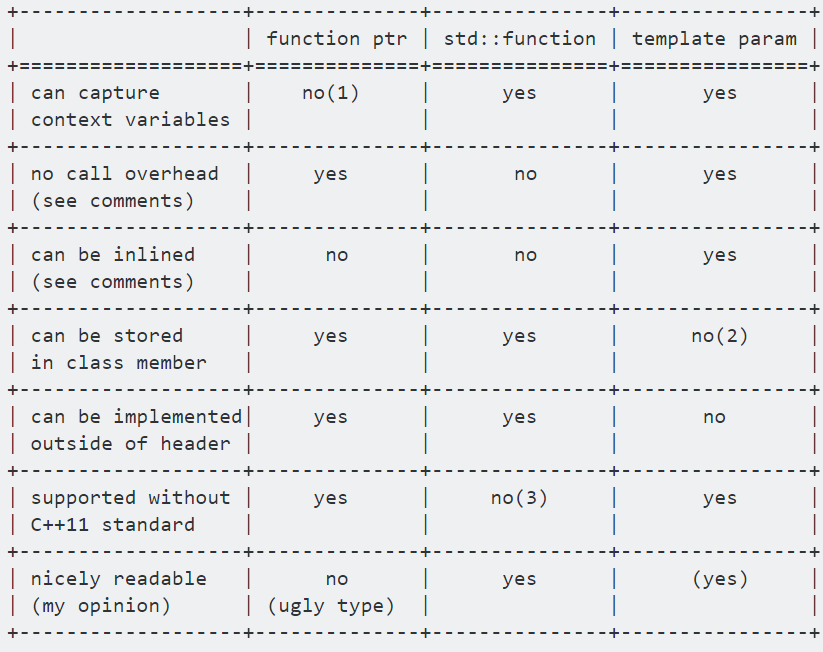
\includegraphics[scale=0.45]{pics/function.png} \newline
\end{itemize}


\subsection{Other New Feature}
\subsubsection{constexpr}
\begin{itemize}

\item Unlike templates and preprocessor macros, constexpr allows for loops and recursion at compile-time without extreme boilerplate.

\item constexpr functions can be used as regular functions, although internally they have greater restrictions.

\item constexpr functions can easily be converted into regular functions as requirements change.

\item constexpr functions compile much quicker than the equivalent template-based solutions, which scale linearly with the depth of the template-recursion.

\item The basic idea is "compile time input yields compile time output". How can I know if a function is constexpr or not? 

\item std::find is constexpr function now. 

\item the question is : when should you use constexpr? The answer is the same than with const: as much as you can.

\item The most powerful thing about constant expressions, is that they enable you to do meta-programming without resorting to templates.

\item A good artical is "Demystifying constexpr". 
\end{itemize}

\subsubsection{alias declaration}

\begin{itemize}
\item Alias declaration is better than typedef when you declare a function pointer, It's more verbose.
\begin{lstlisting}[frame=single, language=c++]
// FP is a synonym for a pointer to a function taking an int
// and a const std::string& and returning nothing
typedef void (*FP)(int, const std::string&);

using FP = void (*)(int, const std::string&);
// alias declaration
\end{lstlisting}

\item C++11 doesn't support typedef template directly, only can be put inside a struct.
\begin{lstlisting}[frame=single, language=c++]
template<typename T> // MyAllocList<T>
using MyAllocList = std::list<T, MyAlloc<T>>;
// is synonym for std::list<T, MyAlloc<T>>
MyAllocList<Widget> lw; // client code

template<typename T>
struct MyAllocList {
typedef std::list<T, MyAlloc<T>> type;
};
// MyAllocList<T>::type is synonym for std::list<T,  MyAlloc<T>>
MyAllocList<Widget>::type lw; // client code
\end{lstlisting}

\item MyAllocList<T>::type is thus a dependent type, and one of C++'s many endearing rules is that the names of dependent types must be preceded by typename.

\begin{lstlisting}[frame=single, language=c++]
template<typename T>
class Widget { // Widget<T> contains
private: // a MyAllocList<T>
typename MyAllocList<T>::type list; // as a data member
};
\end{lstlisting}
\item A better way is to use Alias name
\begin{lstlisting}[frame=single, language=c++]
template<typename T>
using MyAllocList = std::list<T, MyAlloc<T>>; // as before

template<typename T>
class Widget {
private:
MyAllocList<T> list; // no "typename" and no "::type"
};
\end{lstlisting}

\item Another advantage of Alias Name is below:

\begin{lstlisting}[frame=single, language=c++]
template<typename T>
struct type{ typedef std::vector<T> sometype; }

template<typename TT>
void someFunction( typename type<TT>::sometype& myArg );
//You need typename here, because sometype is depended T.
//typename indicates type<TT>::sometype is a type.

std::vector<int> a;
someFunction(a); // error, cannot deduce 'TT'
someFunction<int>(a);


template<typename T>
using sometype = std::vector<T>;

template<typename T>
void someFunction(sometype<T> &myArg );

std::vector<int> a;
someFunction(a);
\end{lstlisting}

\item C++14 offers alias templates for all the C++11 type traits transformations.
\begin{lstlisting}[frame=single, language=c++]
template <class T>
using remove_const_t = typename remove_const<T>::type;
template <class T>
using remove_reference_t = typename remove_reference<T>::type;
template <class T>
using add_lvalue_reference_t =
typename add_lvalue_reference<T>::type;
\end{lstlisting}

\end{itemize}

\subsubsection{scoped enums}
\begin{enumerate}
\item C++98-style enums are now known as unscoped enums.
\begin{lstlisting}[frame=single, language=c++]
enum Color { black, white, red };
// black, white, red are in same scope as Color
auto white = false; // error! white already

enum class Color { black, white, red };
// black, white, red are scoped to Color
auto white = false; // fine, no other

Color c = white; // error!
Color c = Color::white; // fine
auto c = Color::white; // also fine (and in accord
// with Item 5's advice)
\end{lstlisting}

\item Enumerators of scoped enums are visible only within the enum. They convert
to other types only with a cast.
\begin{lstlisting}[frame=single, language=c++]
enum class Color { black, white, red }; // enum is now scoped
Color c = Color::red; // as before, but
... // with scope qualifier
if (c < 14.5) { // error! can't compare
// Color and double
\end{lstlisting}
\item Both scoped and unscoped enums support specification of the underlying type.
The default underlying type for scoped enums is int. Unscoped enums have no
default underlying type.

\item Scoped enums may always be forward-declared. Unscoped enums may be
forward-declared only if their declaration specifies an underlying type.

\item Prefer deleted functions to private undefined ones. because Any function may be deleted, including non-member functions and template instantiations.
\end{enumerate}






\begin{lstlisting}[frame=single, language=c++]
template <class charT, class traits = char_traits<charT> >
class basic_ios : public ios_base {
public:
basic_ios(const basic_ios& ) = delete;
basic_ios& operator=(const basic_ios&) = delete;
};

bool isLucky(int number); // original function
bool isLucky(char) = delete; // reject chars
bool isLucky(bool) = delete; // reject bools

template<typename T>
void processPointer(T* ptr);
template<>
void processPointer<void>(void*) = delete;
//you can't not use void to instantiate
\end{lstlisting} 

\subsubsection{noexcept}

\begin{enumerate}

\item  When an exception is thrown from an noexcept function, std::terminate gets triggered. compiler will not check it for you.

\item noexcept is part of a function's interface, and that means that callers may
depend on it.

\item noexcept functions are more optimizable than non-noexcept functions.

\item noexcept is particularly valuable for the move operations, swap, memory deallocation functions, and destructors.

\item Most functions are exception-neutral rather than noexcept.

\end{enumerate}




\subsubsection{Variadic Templates}
\begin{itemize}
\item Finally, there's a way to write functions that take an arbitrary number of arguments in a type-safe way and have all the argument handling logic resolved at compile-time, rather than run-time.

\begin{lstlisting}[frame=single, language=c++]
template<typename T>
T adder(T v) {
  return v;
}

template<typename T, typename... Args>
T adder(T first, Args... args) {
  return first + adder(args...);
}
////////////////////////////
template<typename T>
show_list(const T& value){cout<<value<<endl;}

template<typename T, typename... Args>
show_list(const T& value, const Args&... args){
cout<<value<<endl;
show_list(args...);
}
\end{lstlisting}

\end{itemize}



%\end{CJK*}
\end{document}

